\section{Real World Classification Tasks}

\subsection{Setup}

Testing hypotheses \textbf{H4} and \textbf{H5}. \textit{\update{Our network architecture will outperform logistic regression in all tested real-world classification datasets.} Our network architecture will approach, but not surpass, the performance of Gradient Boosted Machines on any real-world dataset.}


Experiment four is designed to test our network architecture against other state-of-the-art techniques in real world classification datasets in order to ascertain the importance of joint-terms in this class of problem. Our model is tested against SciKit-Learn logistic and gradient boosting classifiers in binary versions of the Wisconsin Breast Cancer, Sloan Sky Survey, Iris, Titanic, and Wine datasets. In all instances, we compare the f1-scores of all models on all datasets and run statistical significance tests on the results. 

\subsection{Results}

\begin{longtable}[]{@{}llll@{}}
    \toprule
    Dataset & Logistic & GBM & Network\tabularnewline
    \midrule
    \endhead
    Breast Cancer & 0.3592 & \underline{0.9383} & \underline{0.9512}  \tabularnewline
    Sky Survey    & 0.6586 & \underline{0.9871} & \underline{0.9864}  \tabularnewline
    Iris          & 0.3478 & \underline{\textbf{0.9333}} & \underline{0.8966}  \tabularnewline
    Titanic       & 0.7231 & 0.7361 & 0.7200  \tabularnewline
    Wine          & 0.9231 & 0.8718 & 0.9189  \tabularnewline
    \bottomrule
    \caption{Test set F1 scores for each of the models on each of the real-world datasets. Underlined values are statistically significant versus the worst-performing model. Bold values are statistically significant versus to both models.}
\end{longtable}


\begin{figure}[!hp]
    \centering
    \begin{subfigure}{1.0\textwidth}
        \centering
        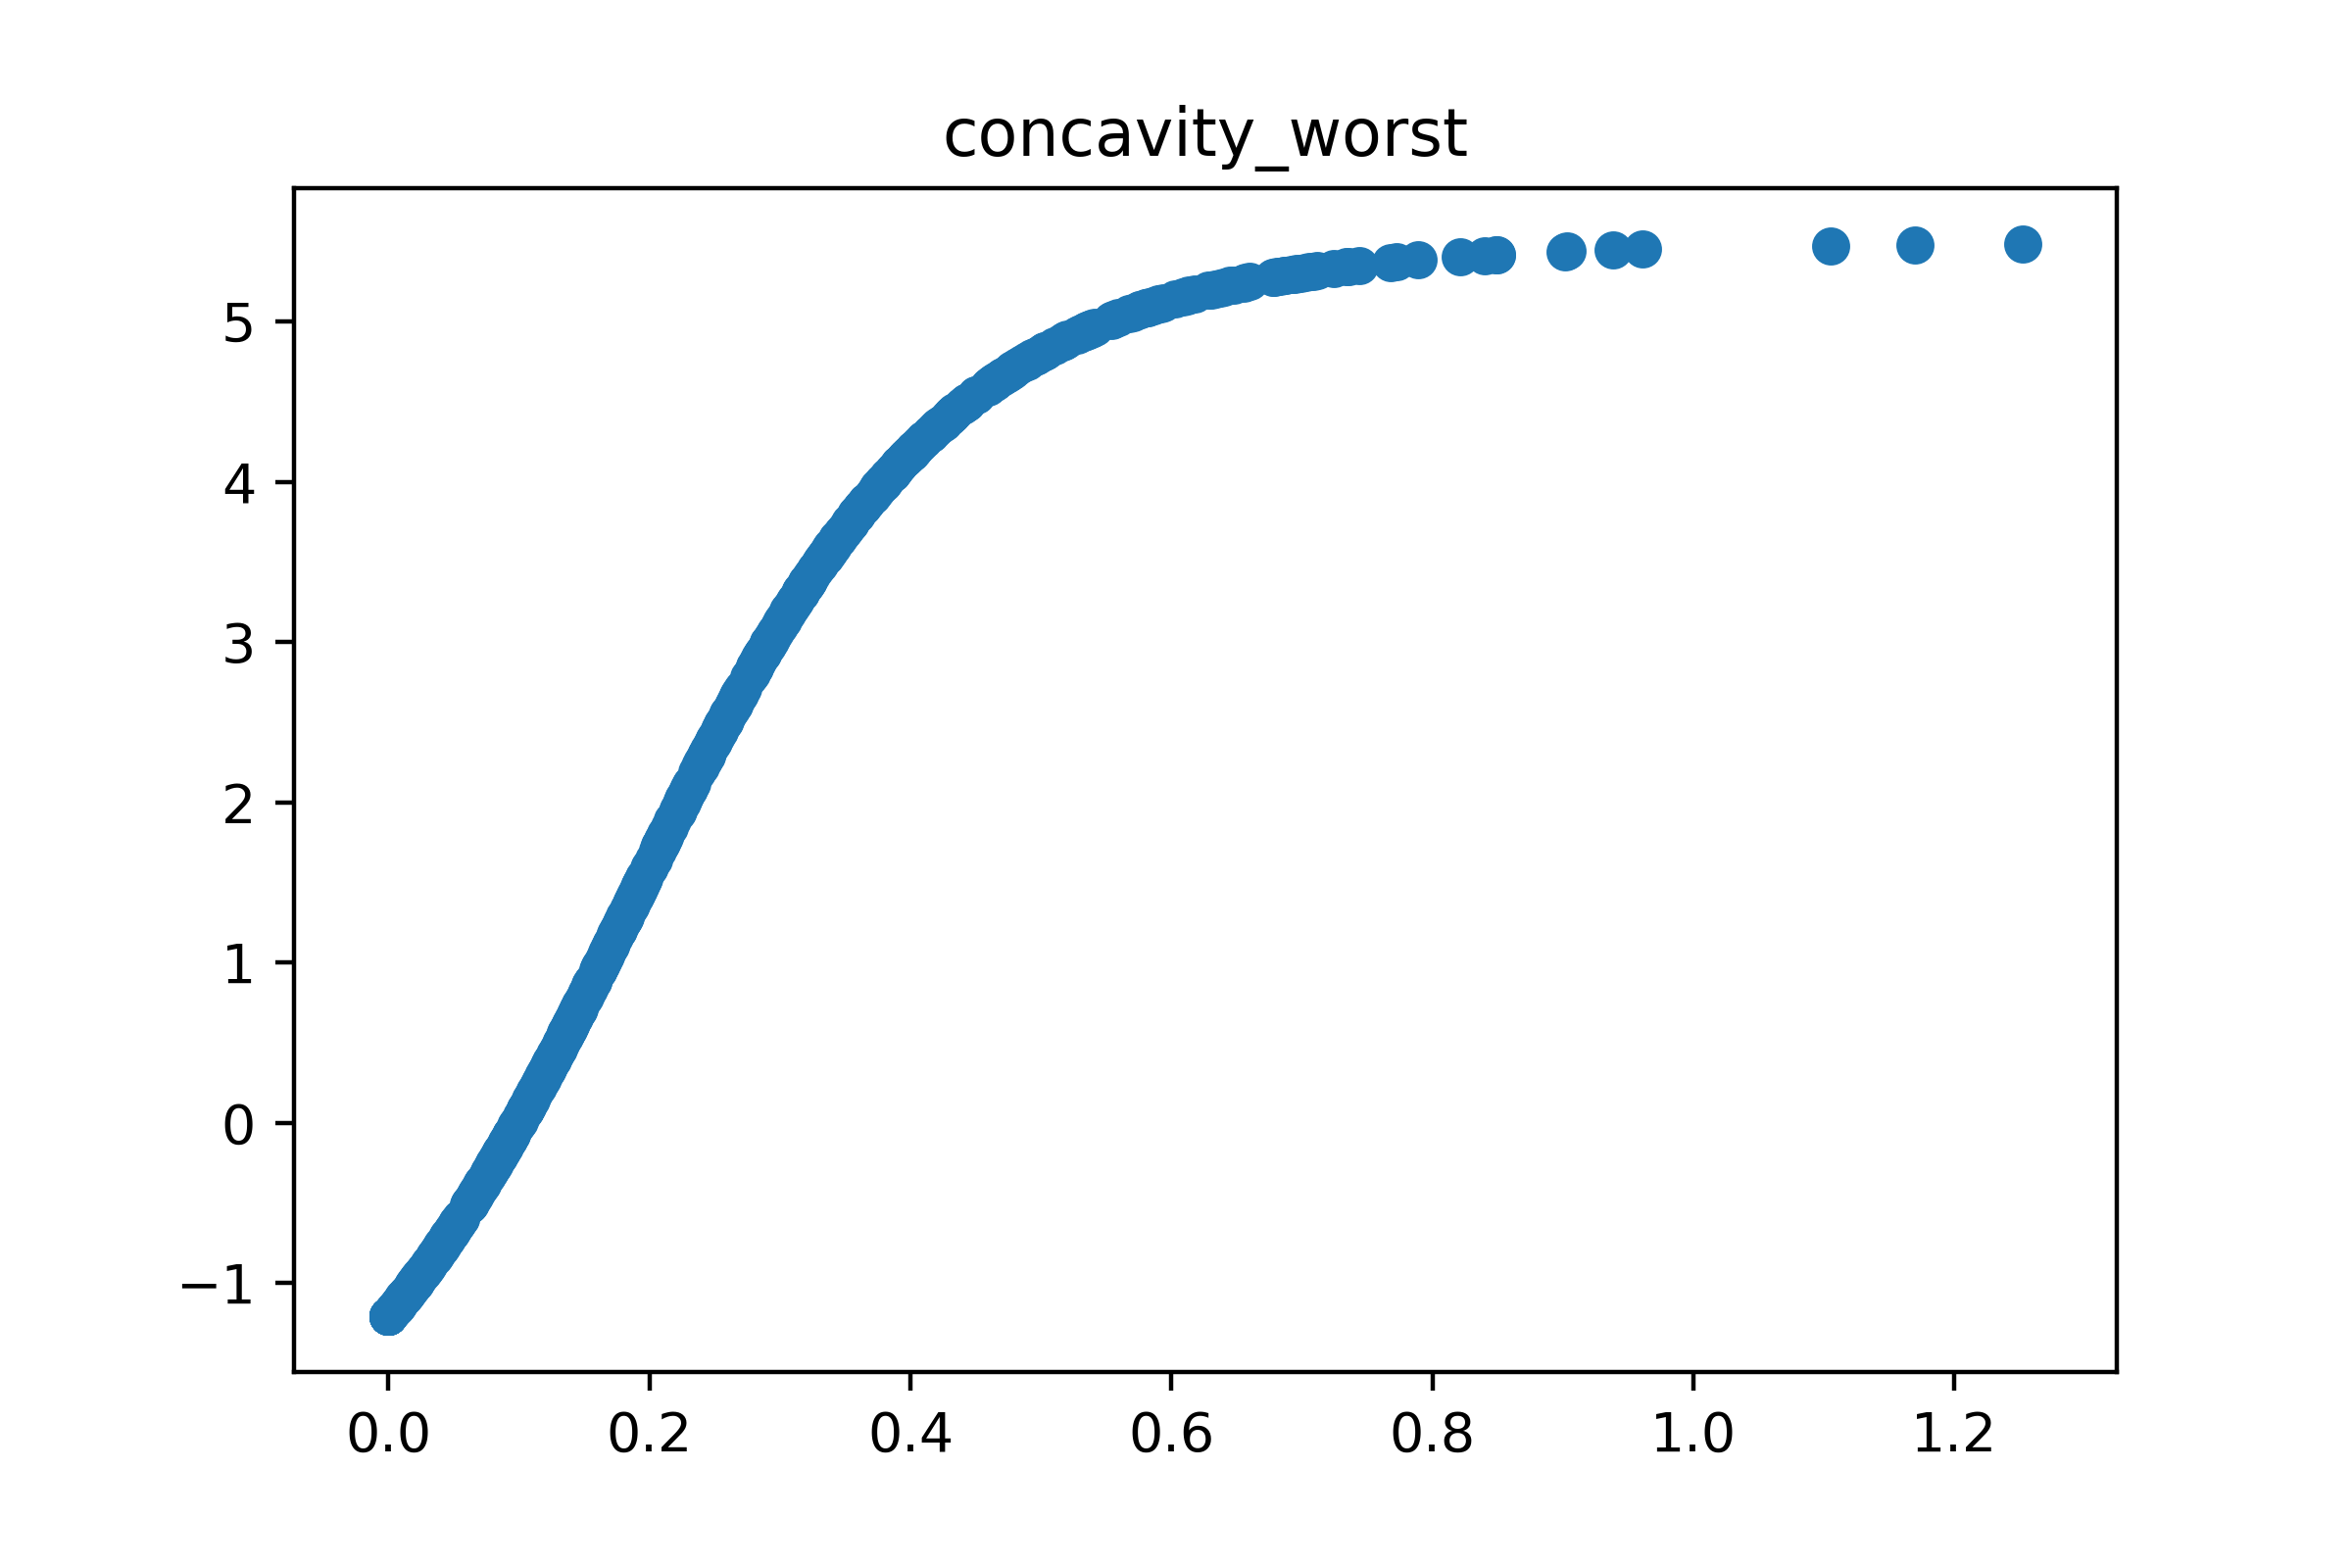
\includegraphics[width=.33\textwidth]{fig/mnl/bc1.png}%
        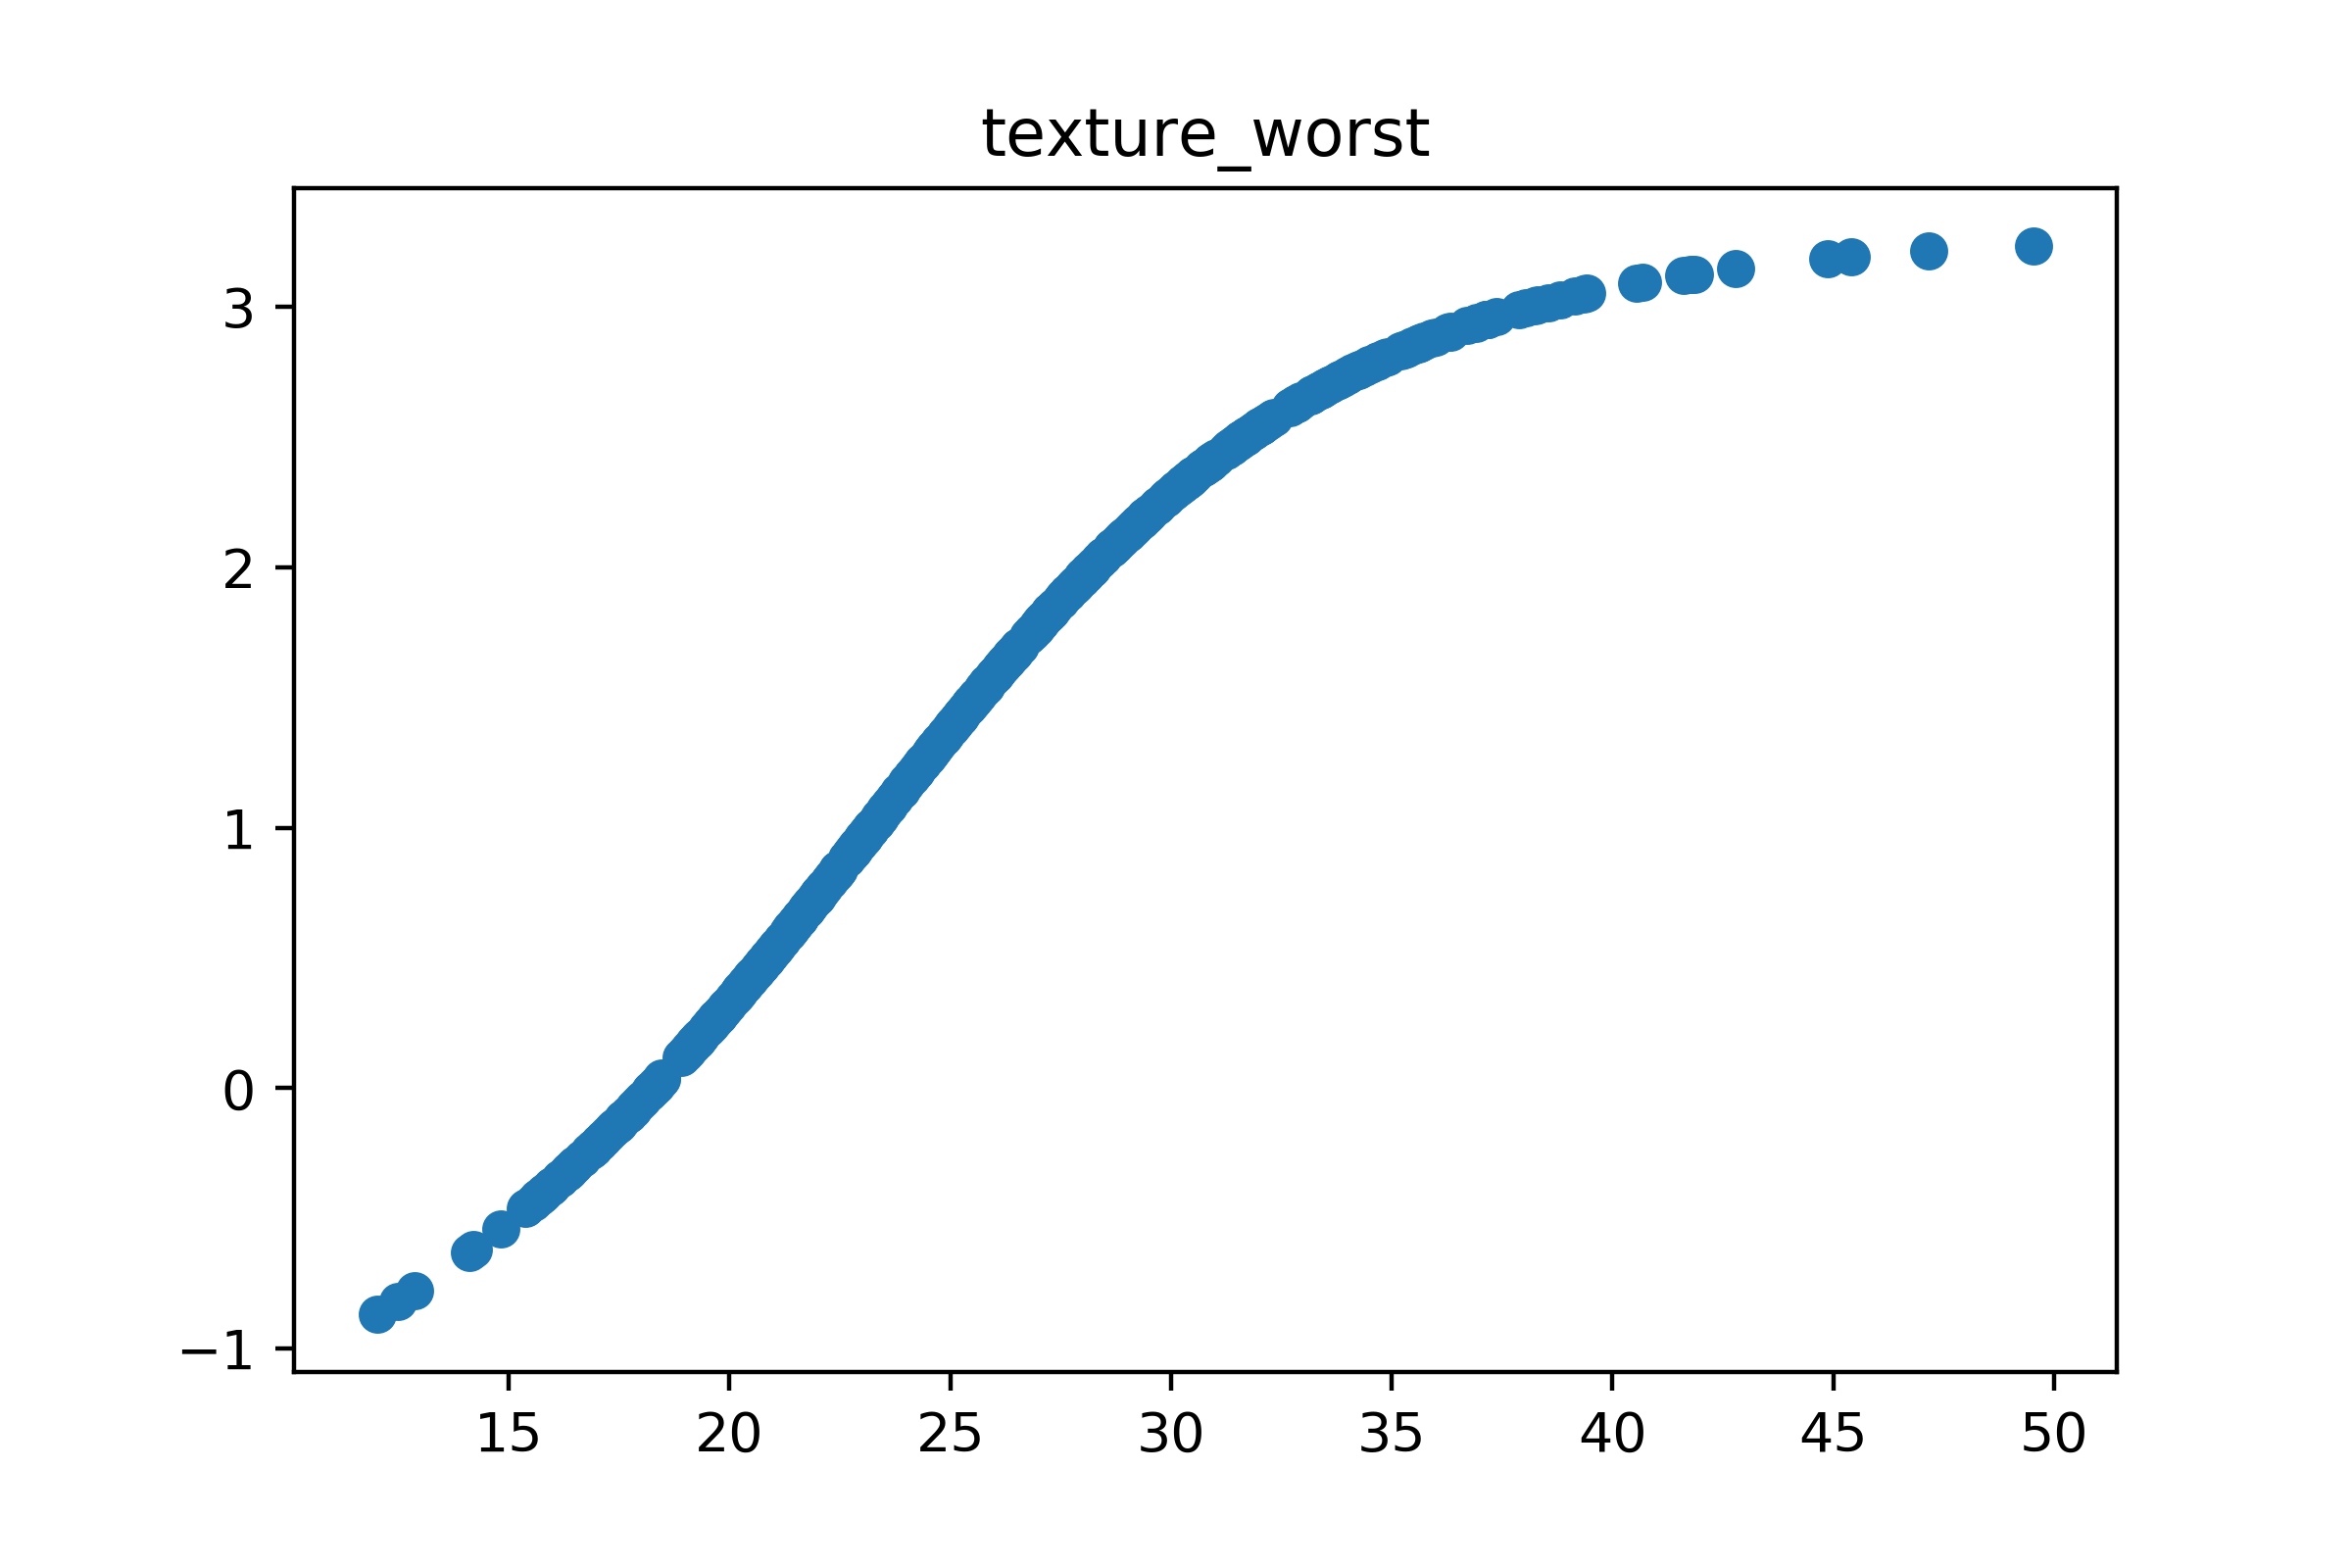
\includegraphics[width=.33\textwidth]{fig/mnl/bc2.png}%
        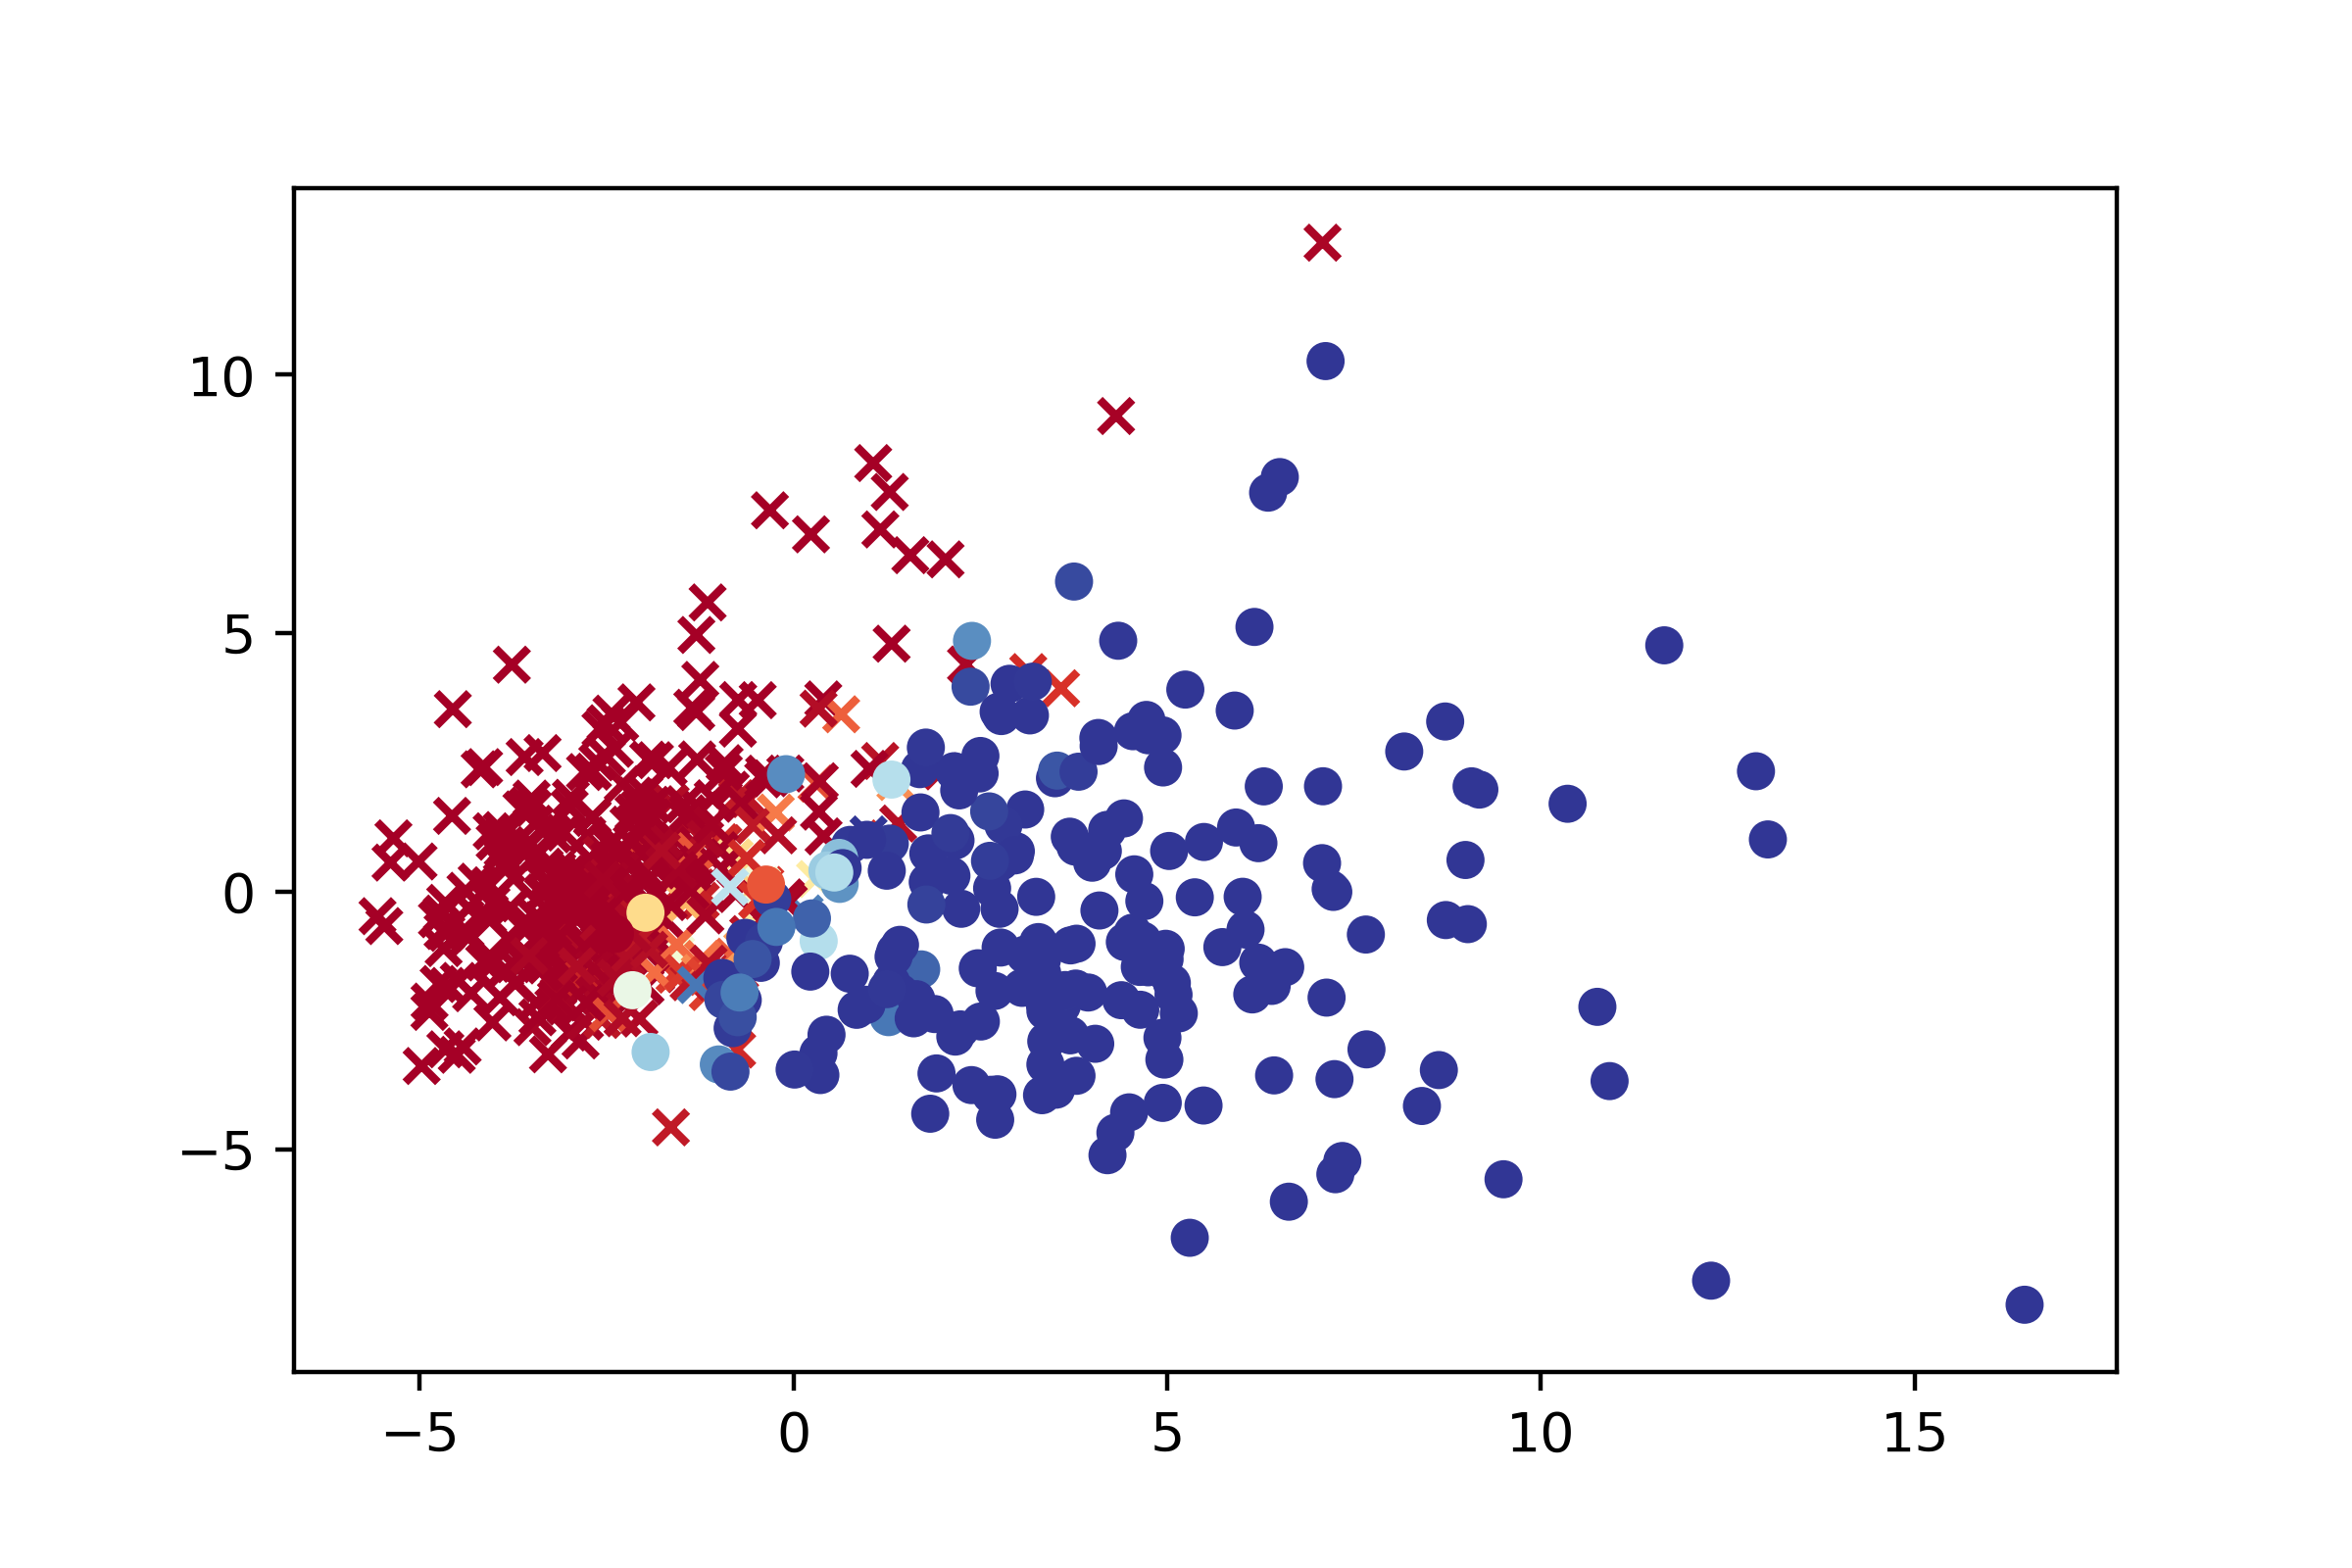
\includegraphics[width=.33\textwidth]{fig/plt/bc.png}
        \caption{Breast Cancer Dataset}
    \end{subfigure}
    \begin{subfigure}{1.0\textwidth}
        \centering
        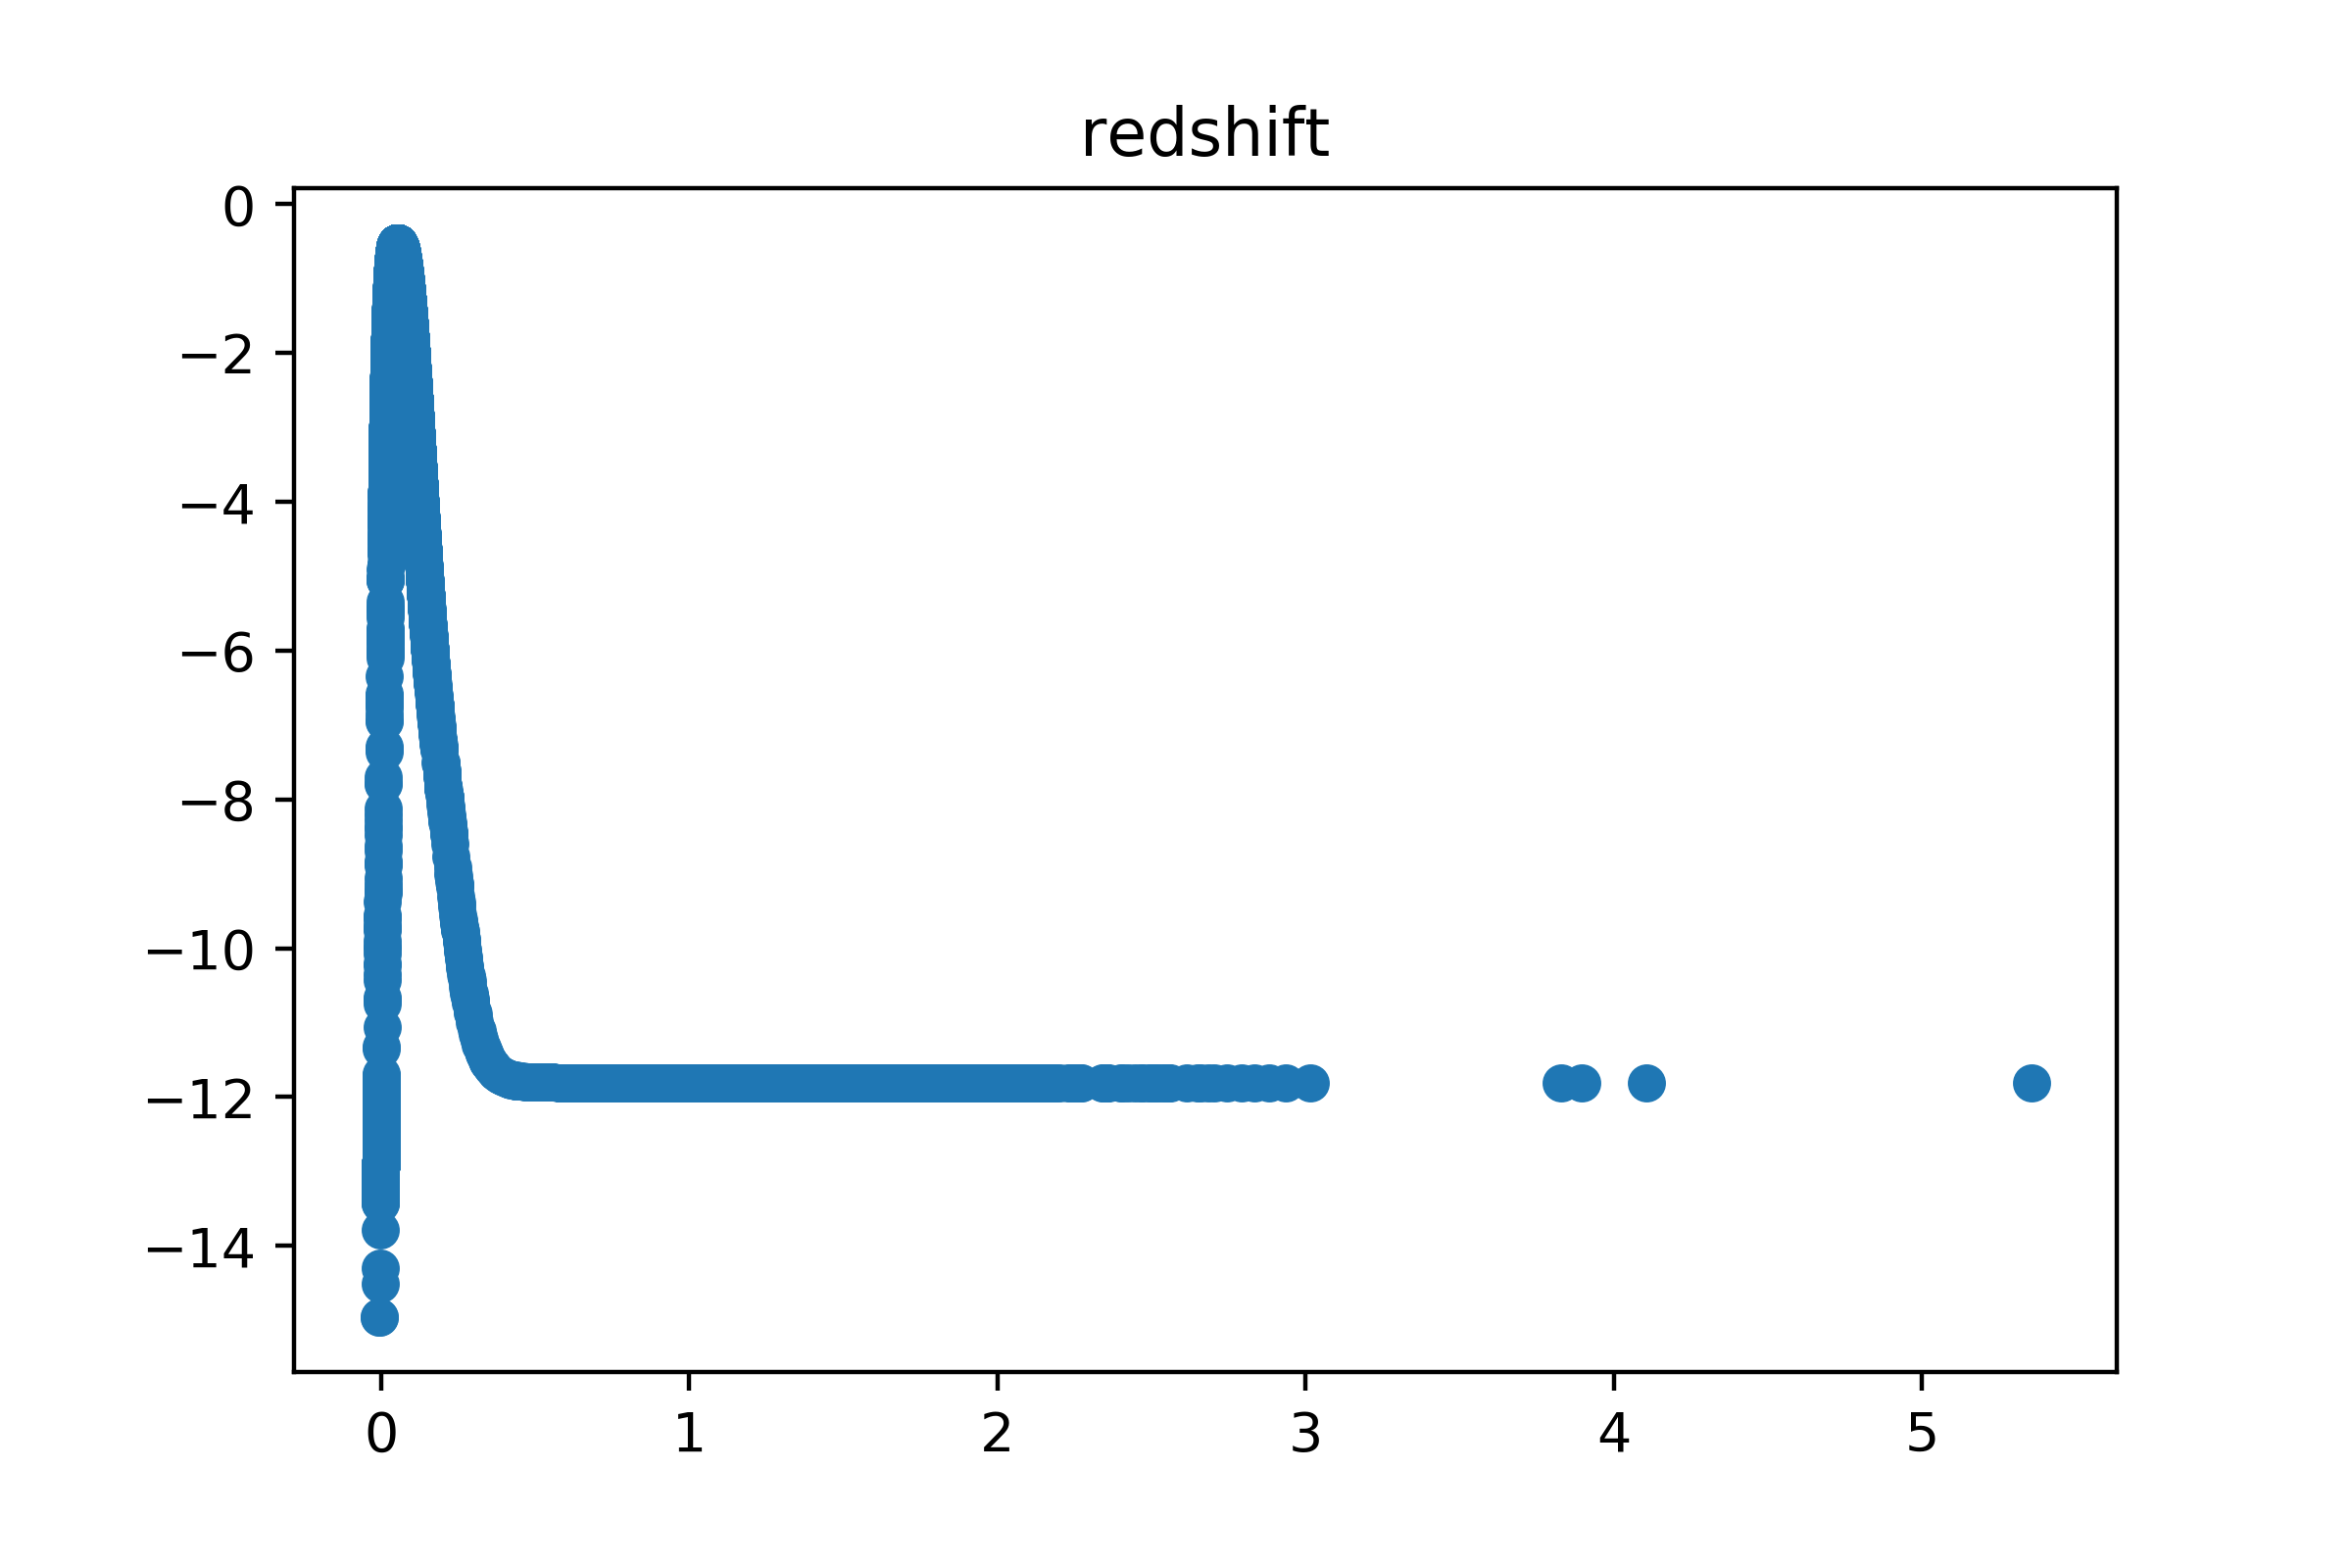
\includegraphics[width=.33\textwidth]{fig/mnl/st1.png}%
        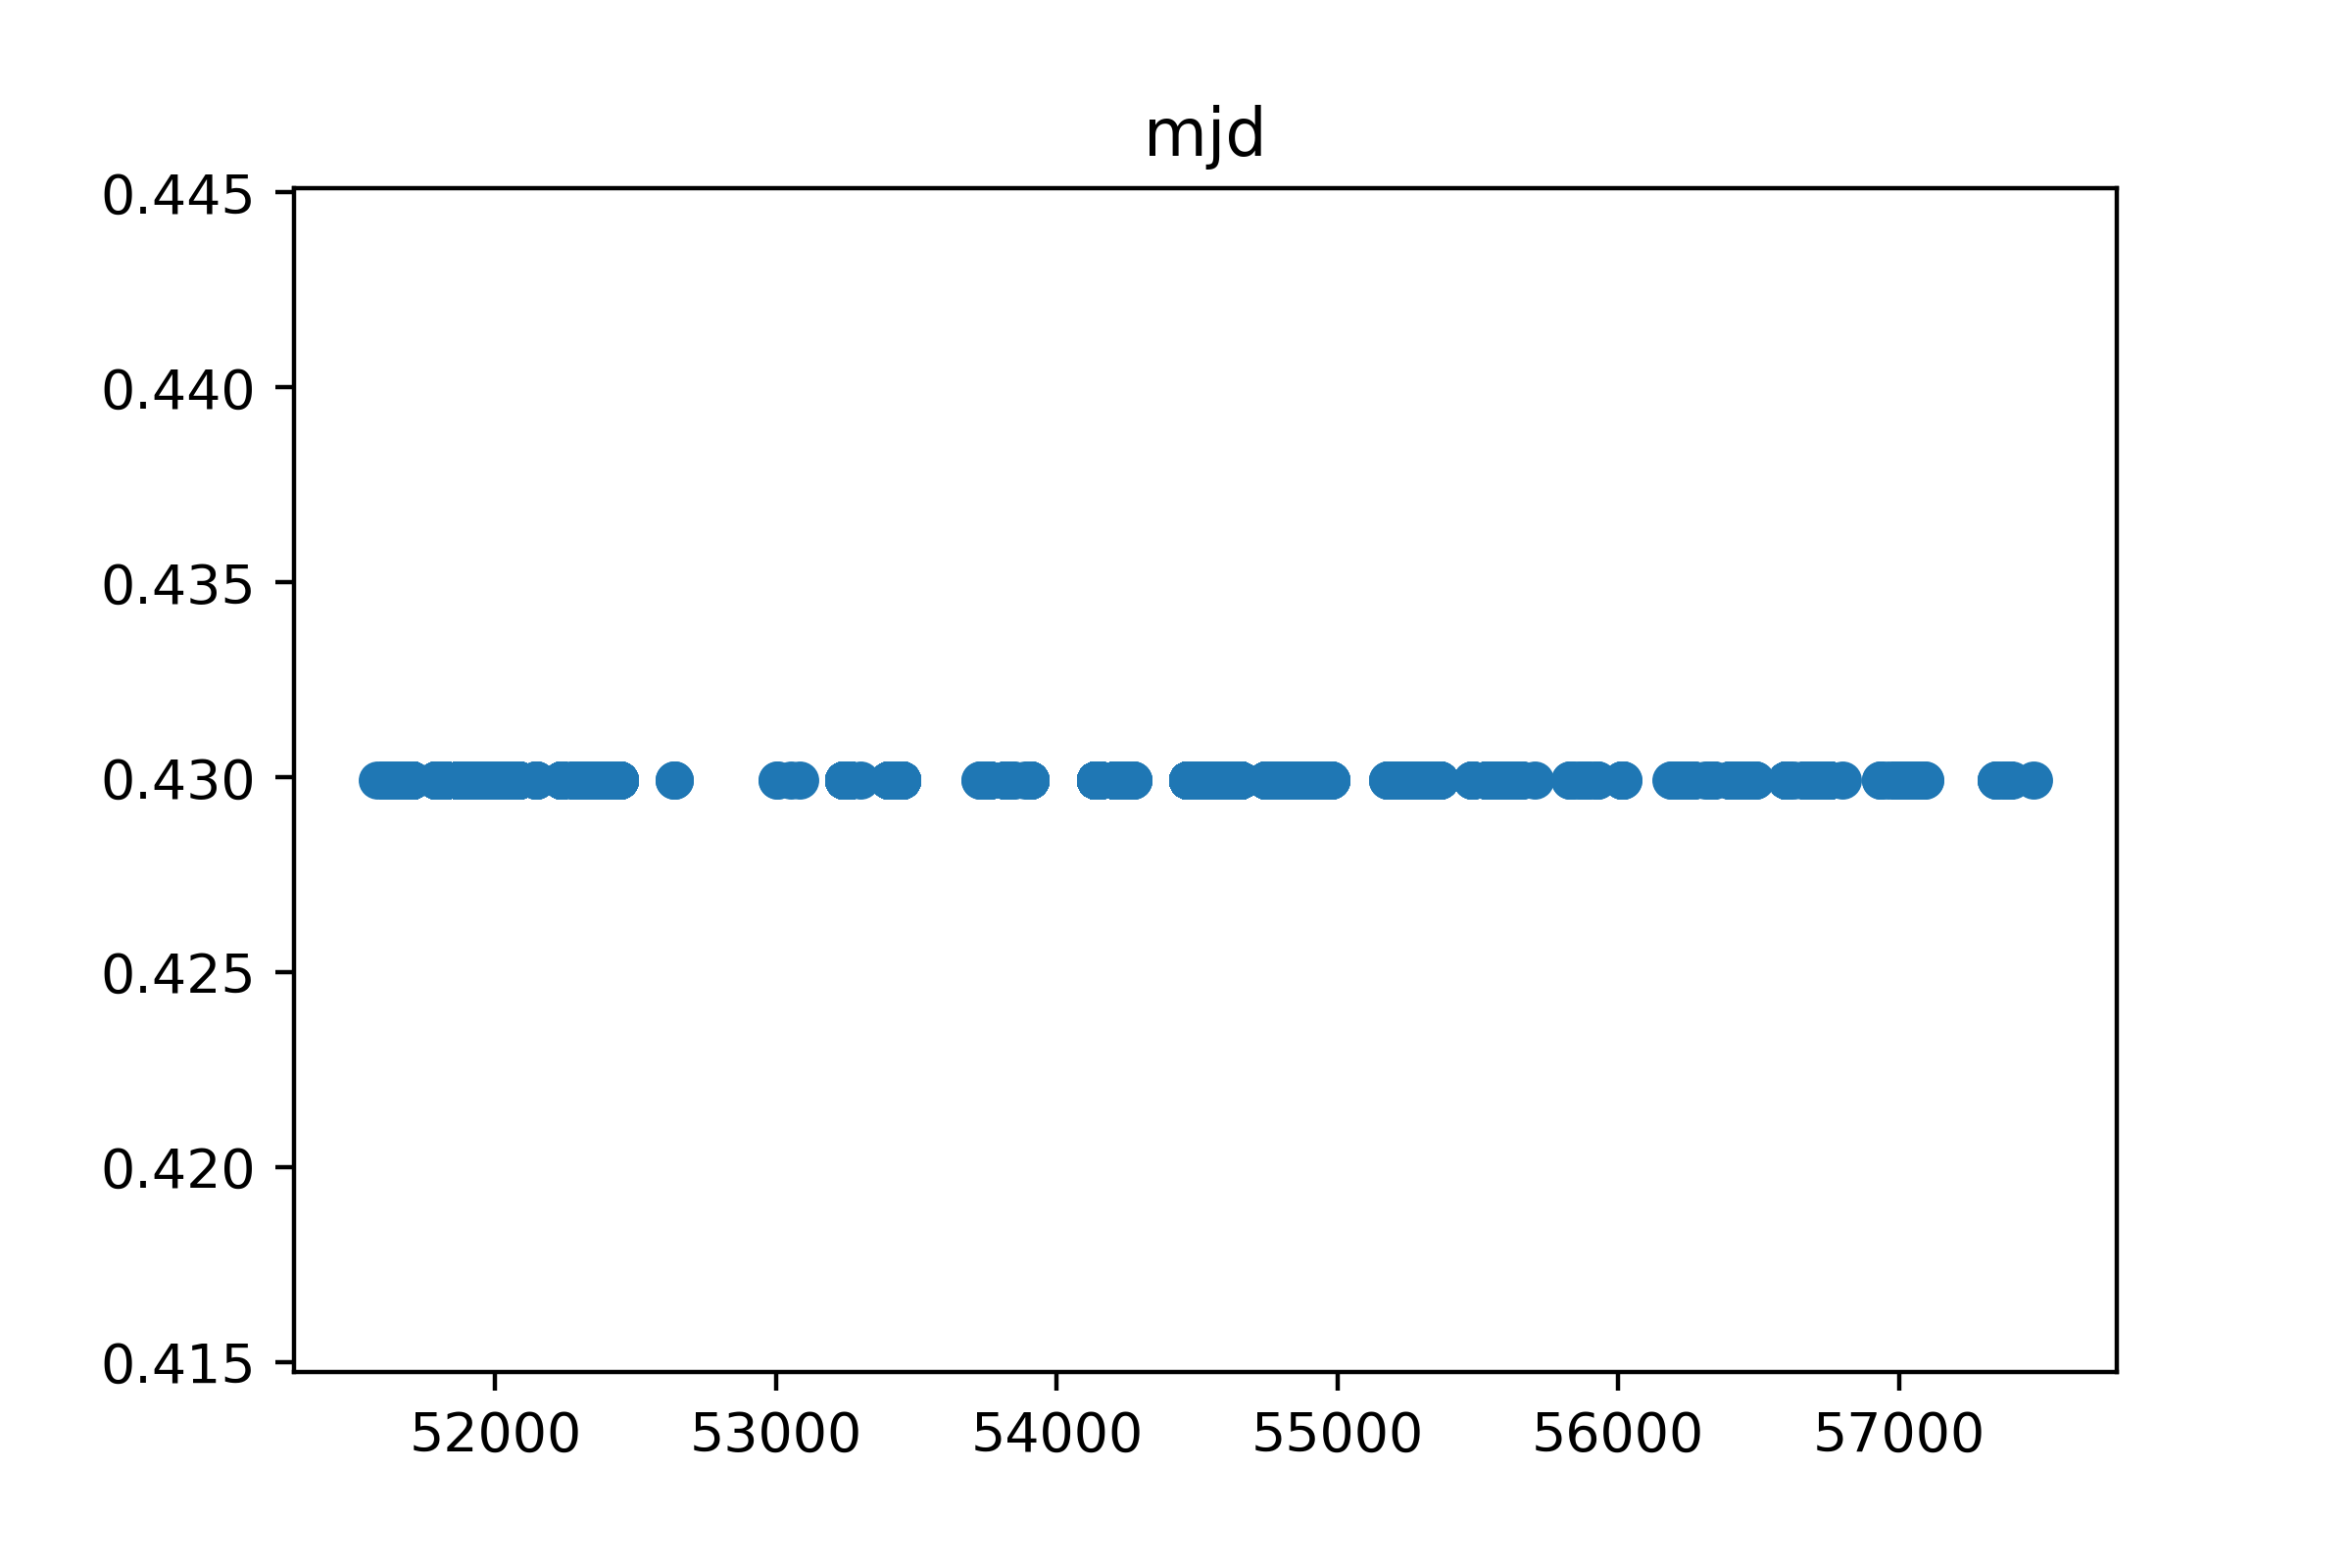
\includegraphics[width=.33\textwidth]{fig/mnl/st2.png}%
        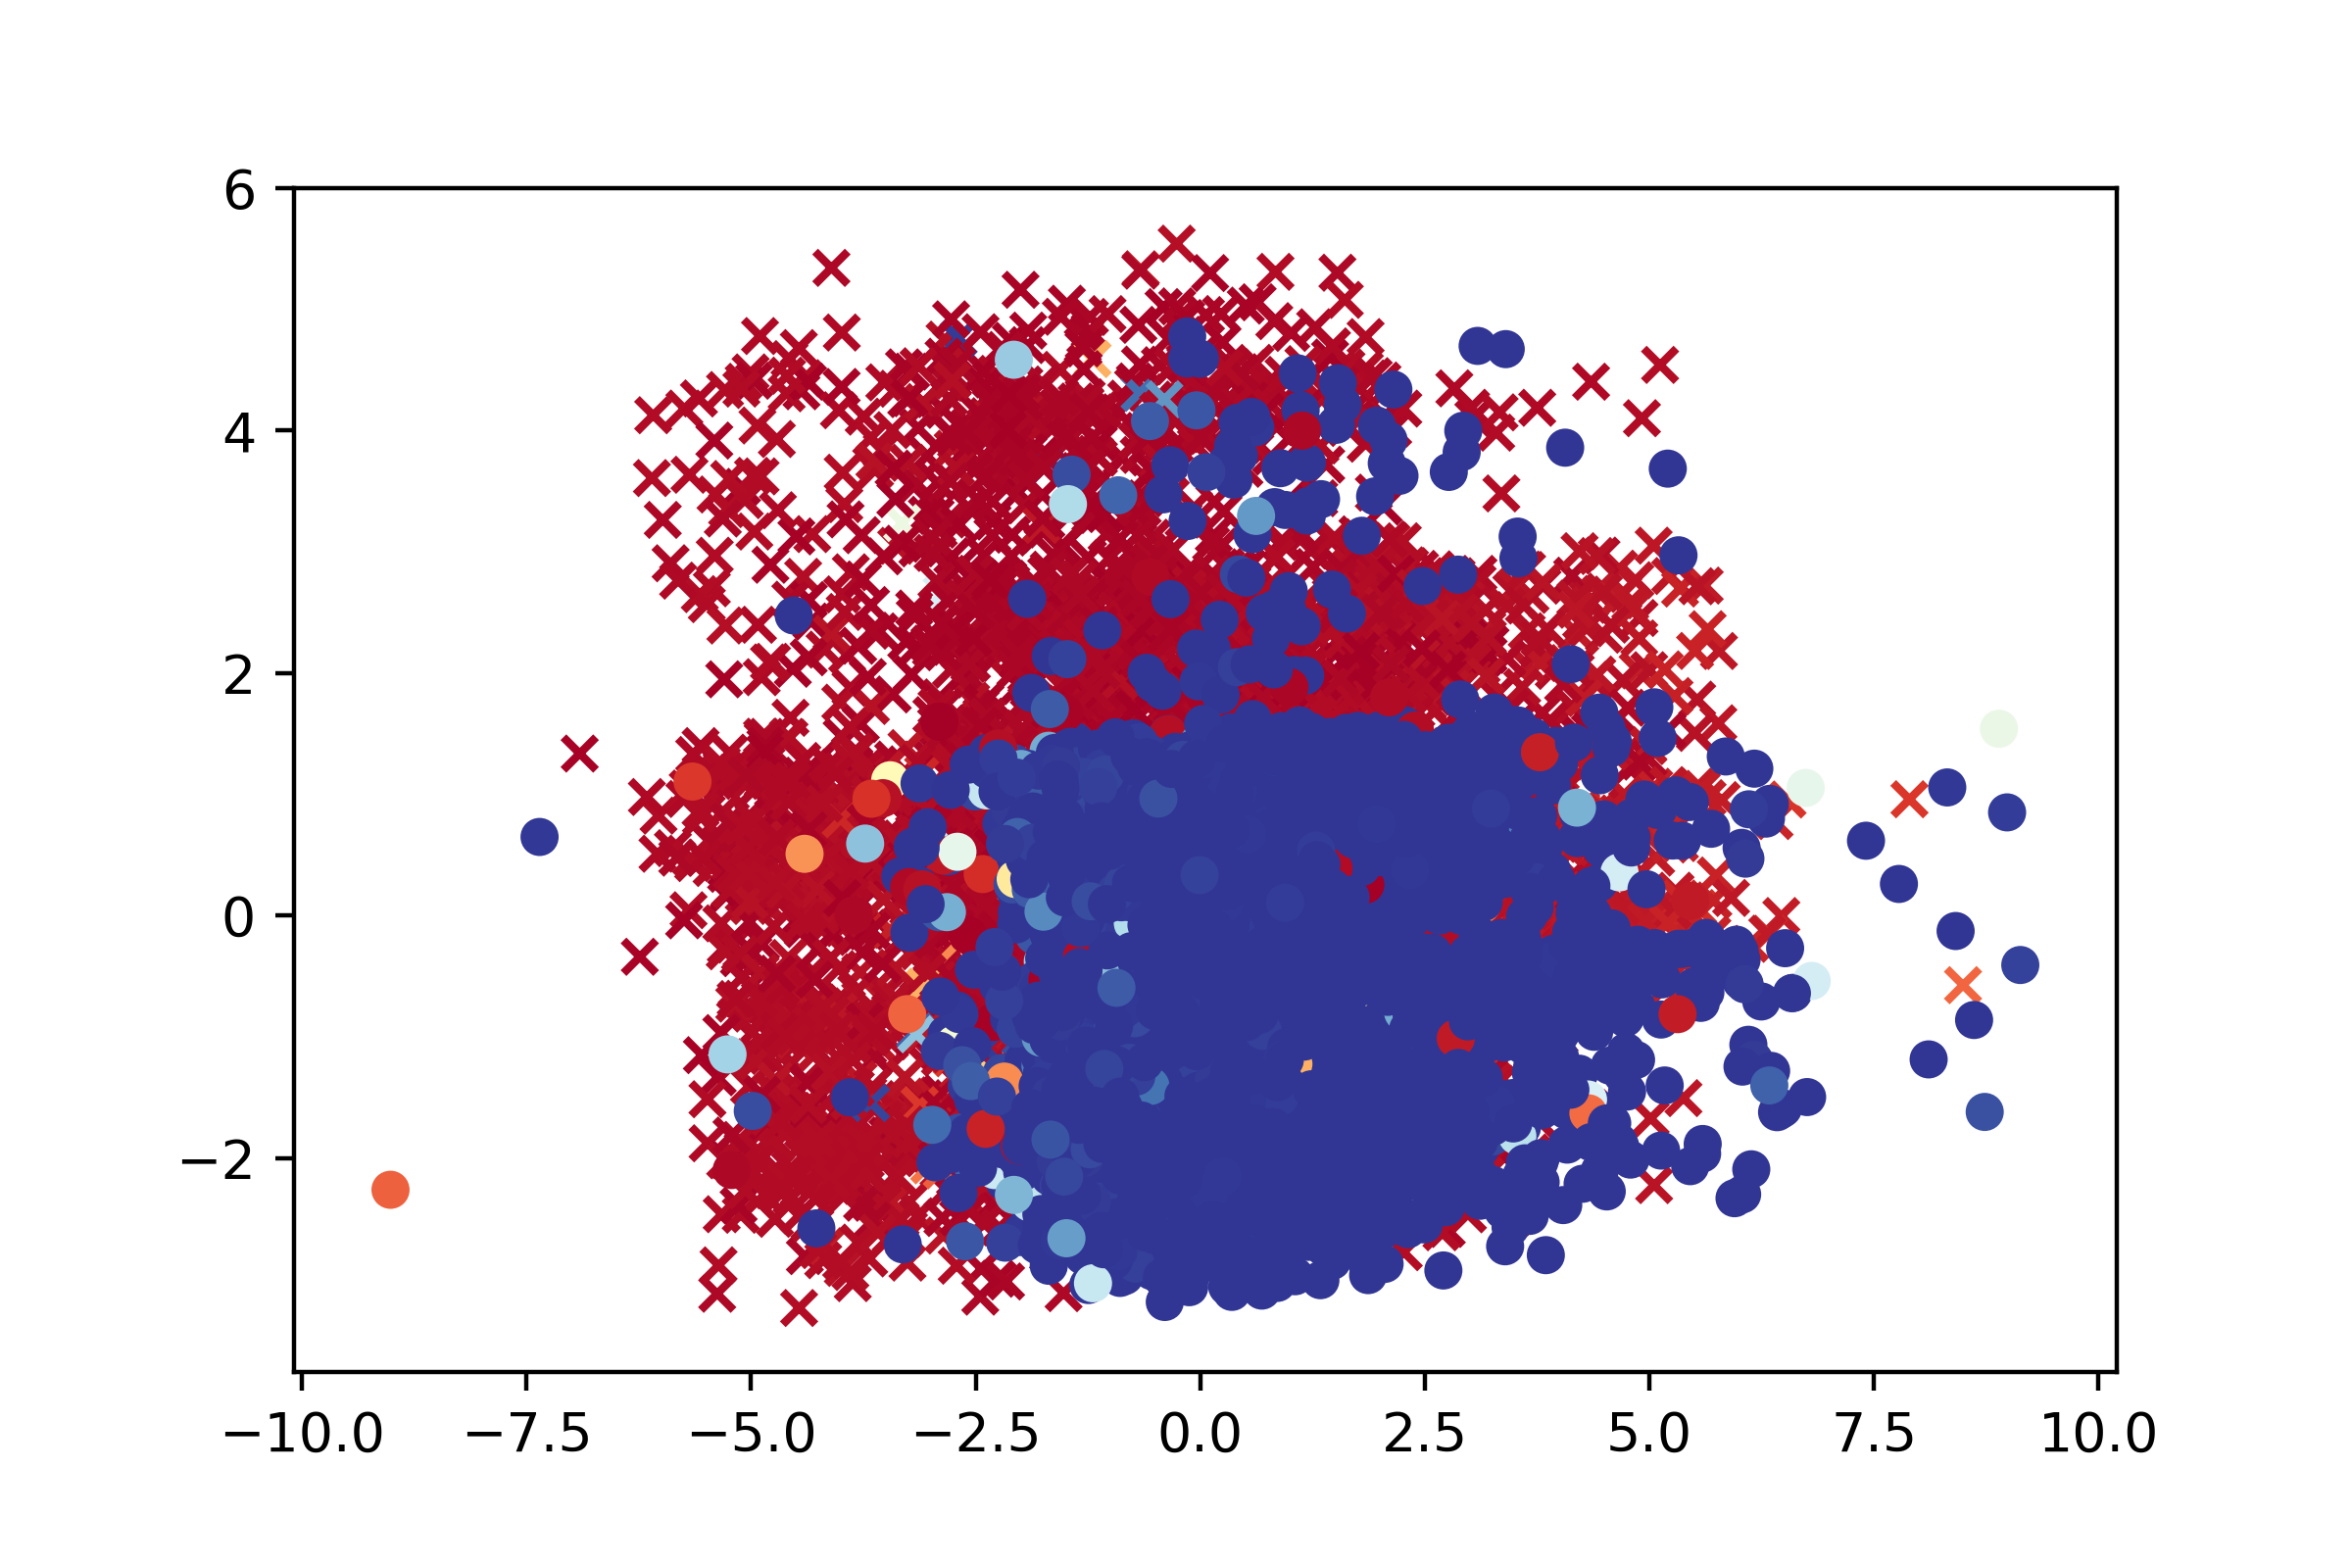
\includegraphics[width=.33\textwidth]{fig/plt/st.png}
        \caption{Sloan Sky Survey Dataset}
    \end{subfigure}
    \begin{subfigure}{1.0\textwidth}
        \centering
        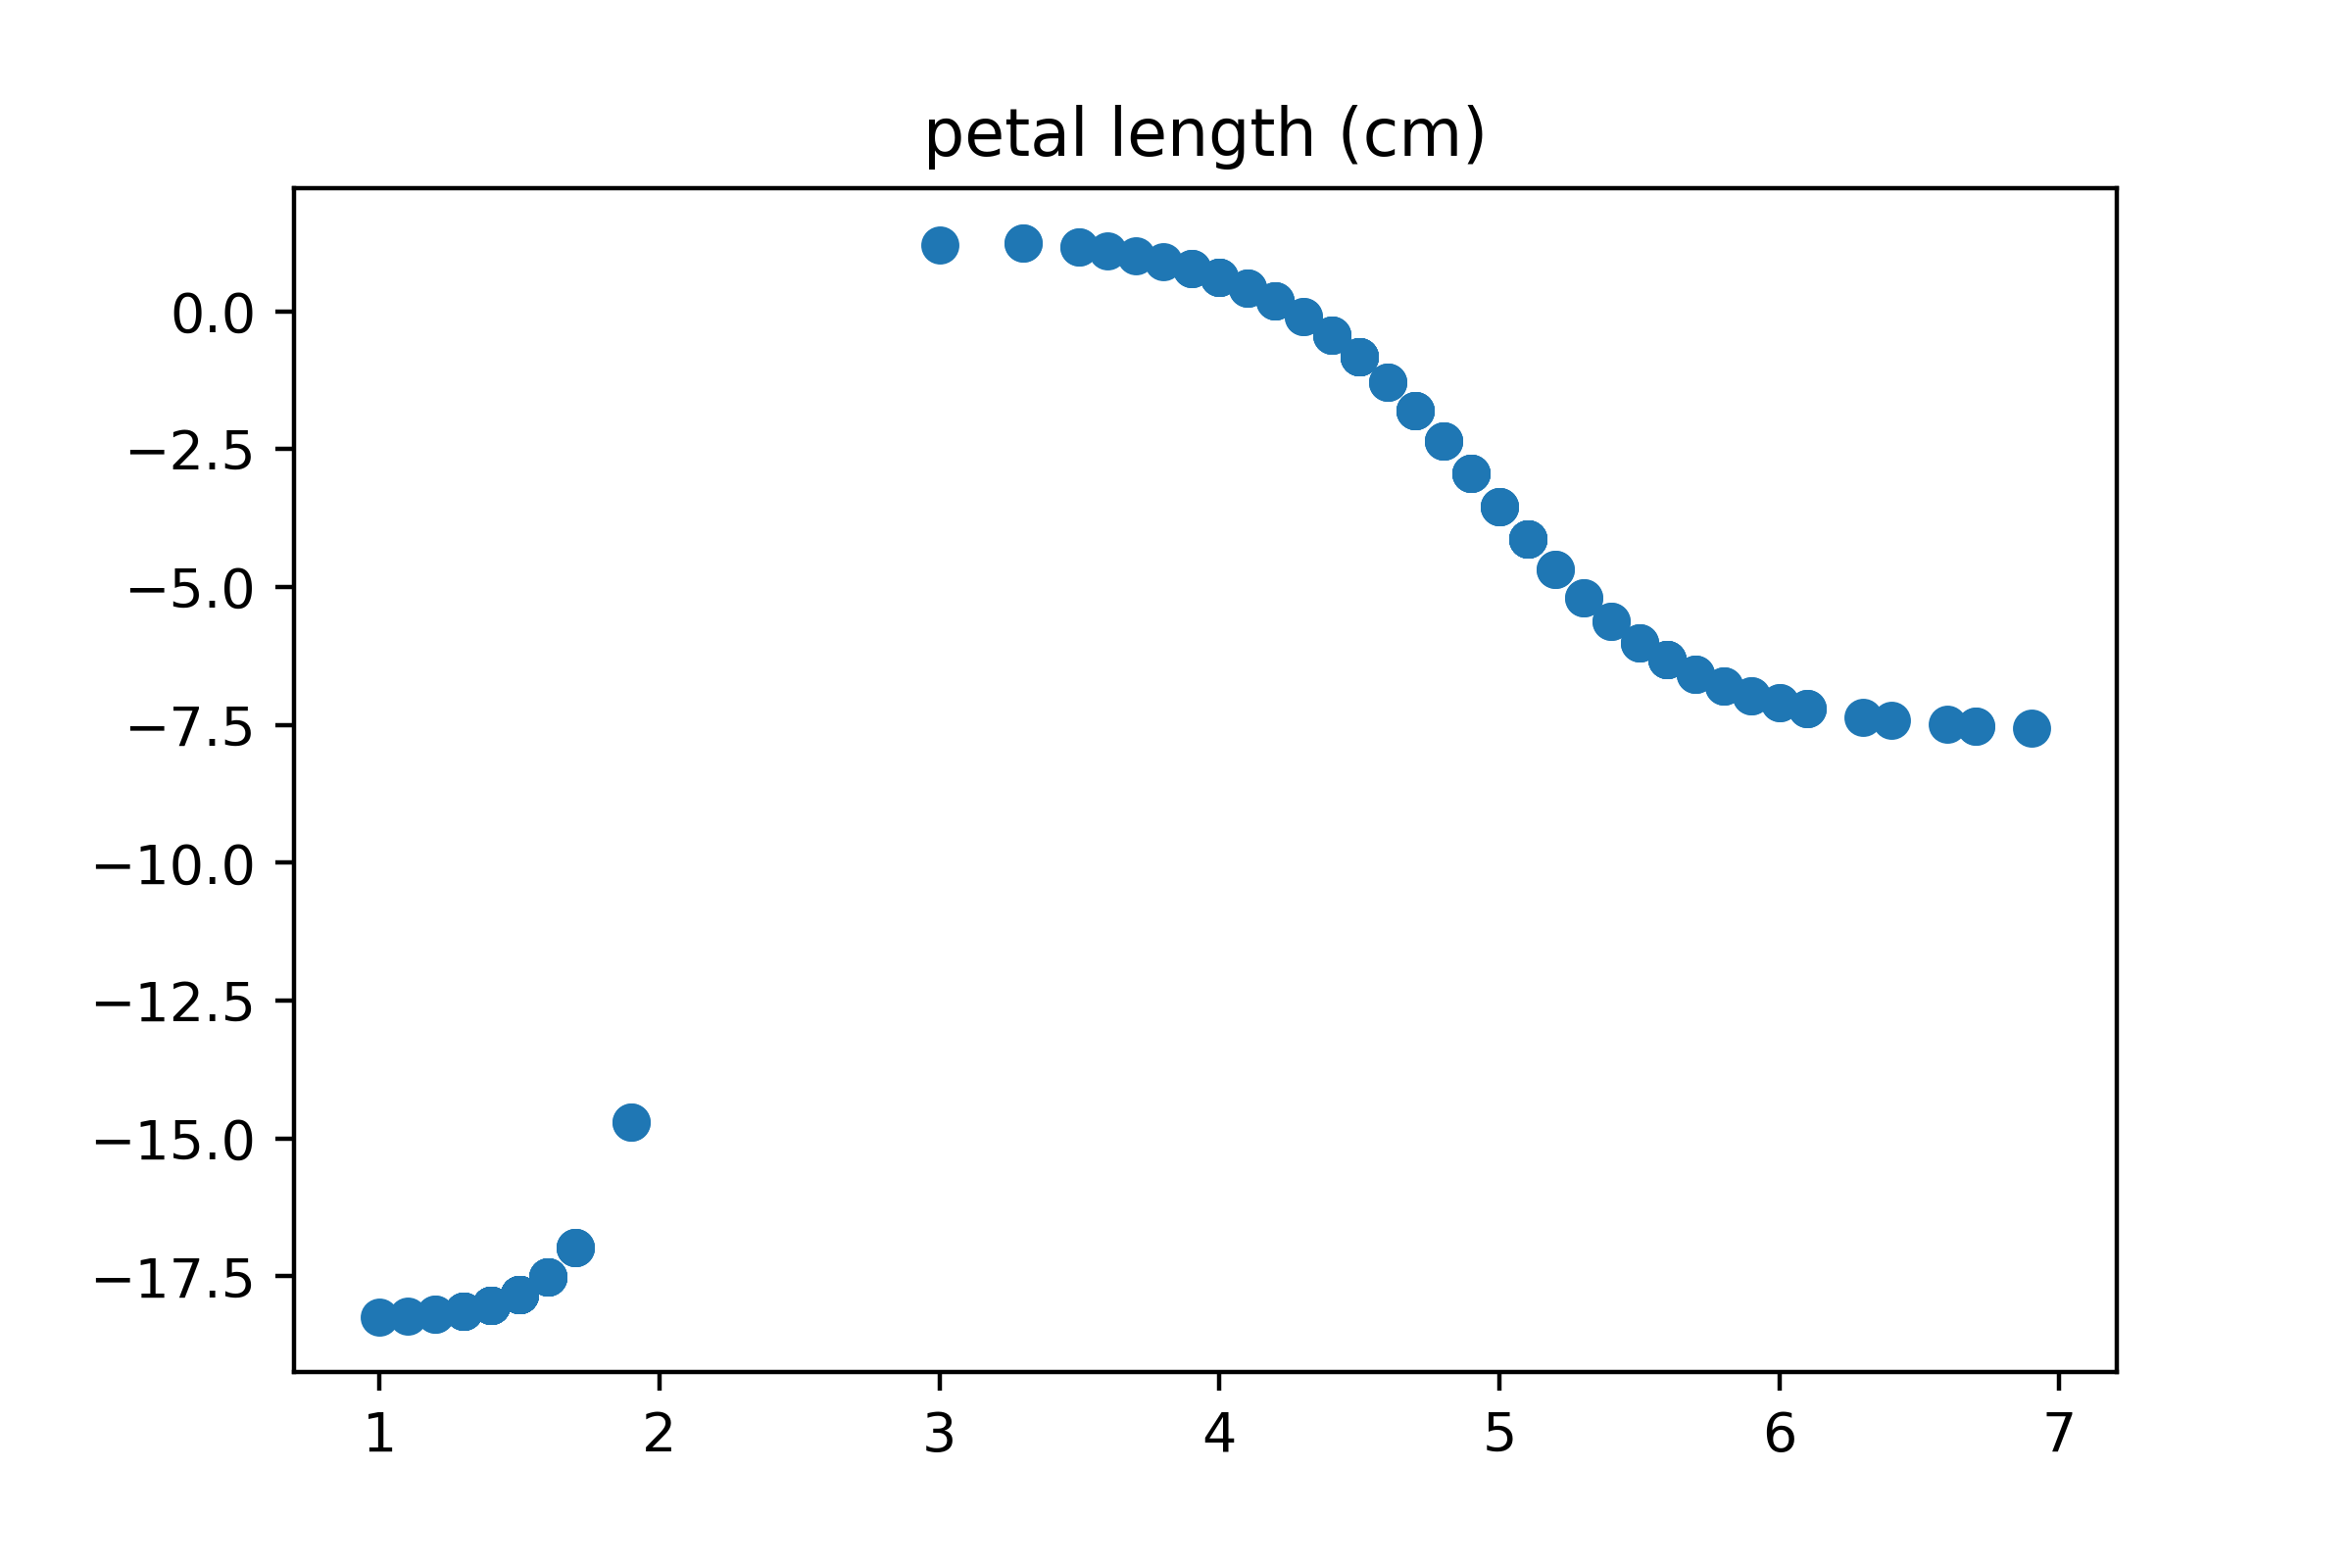
\includegraphics[width=.33\textwidth]{fig/mnl/ir1.png}%
        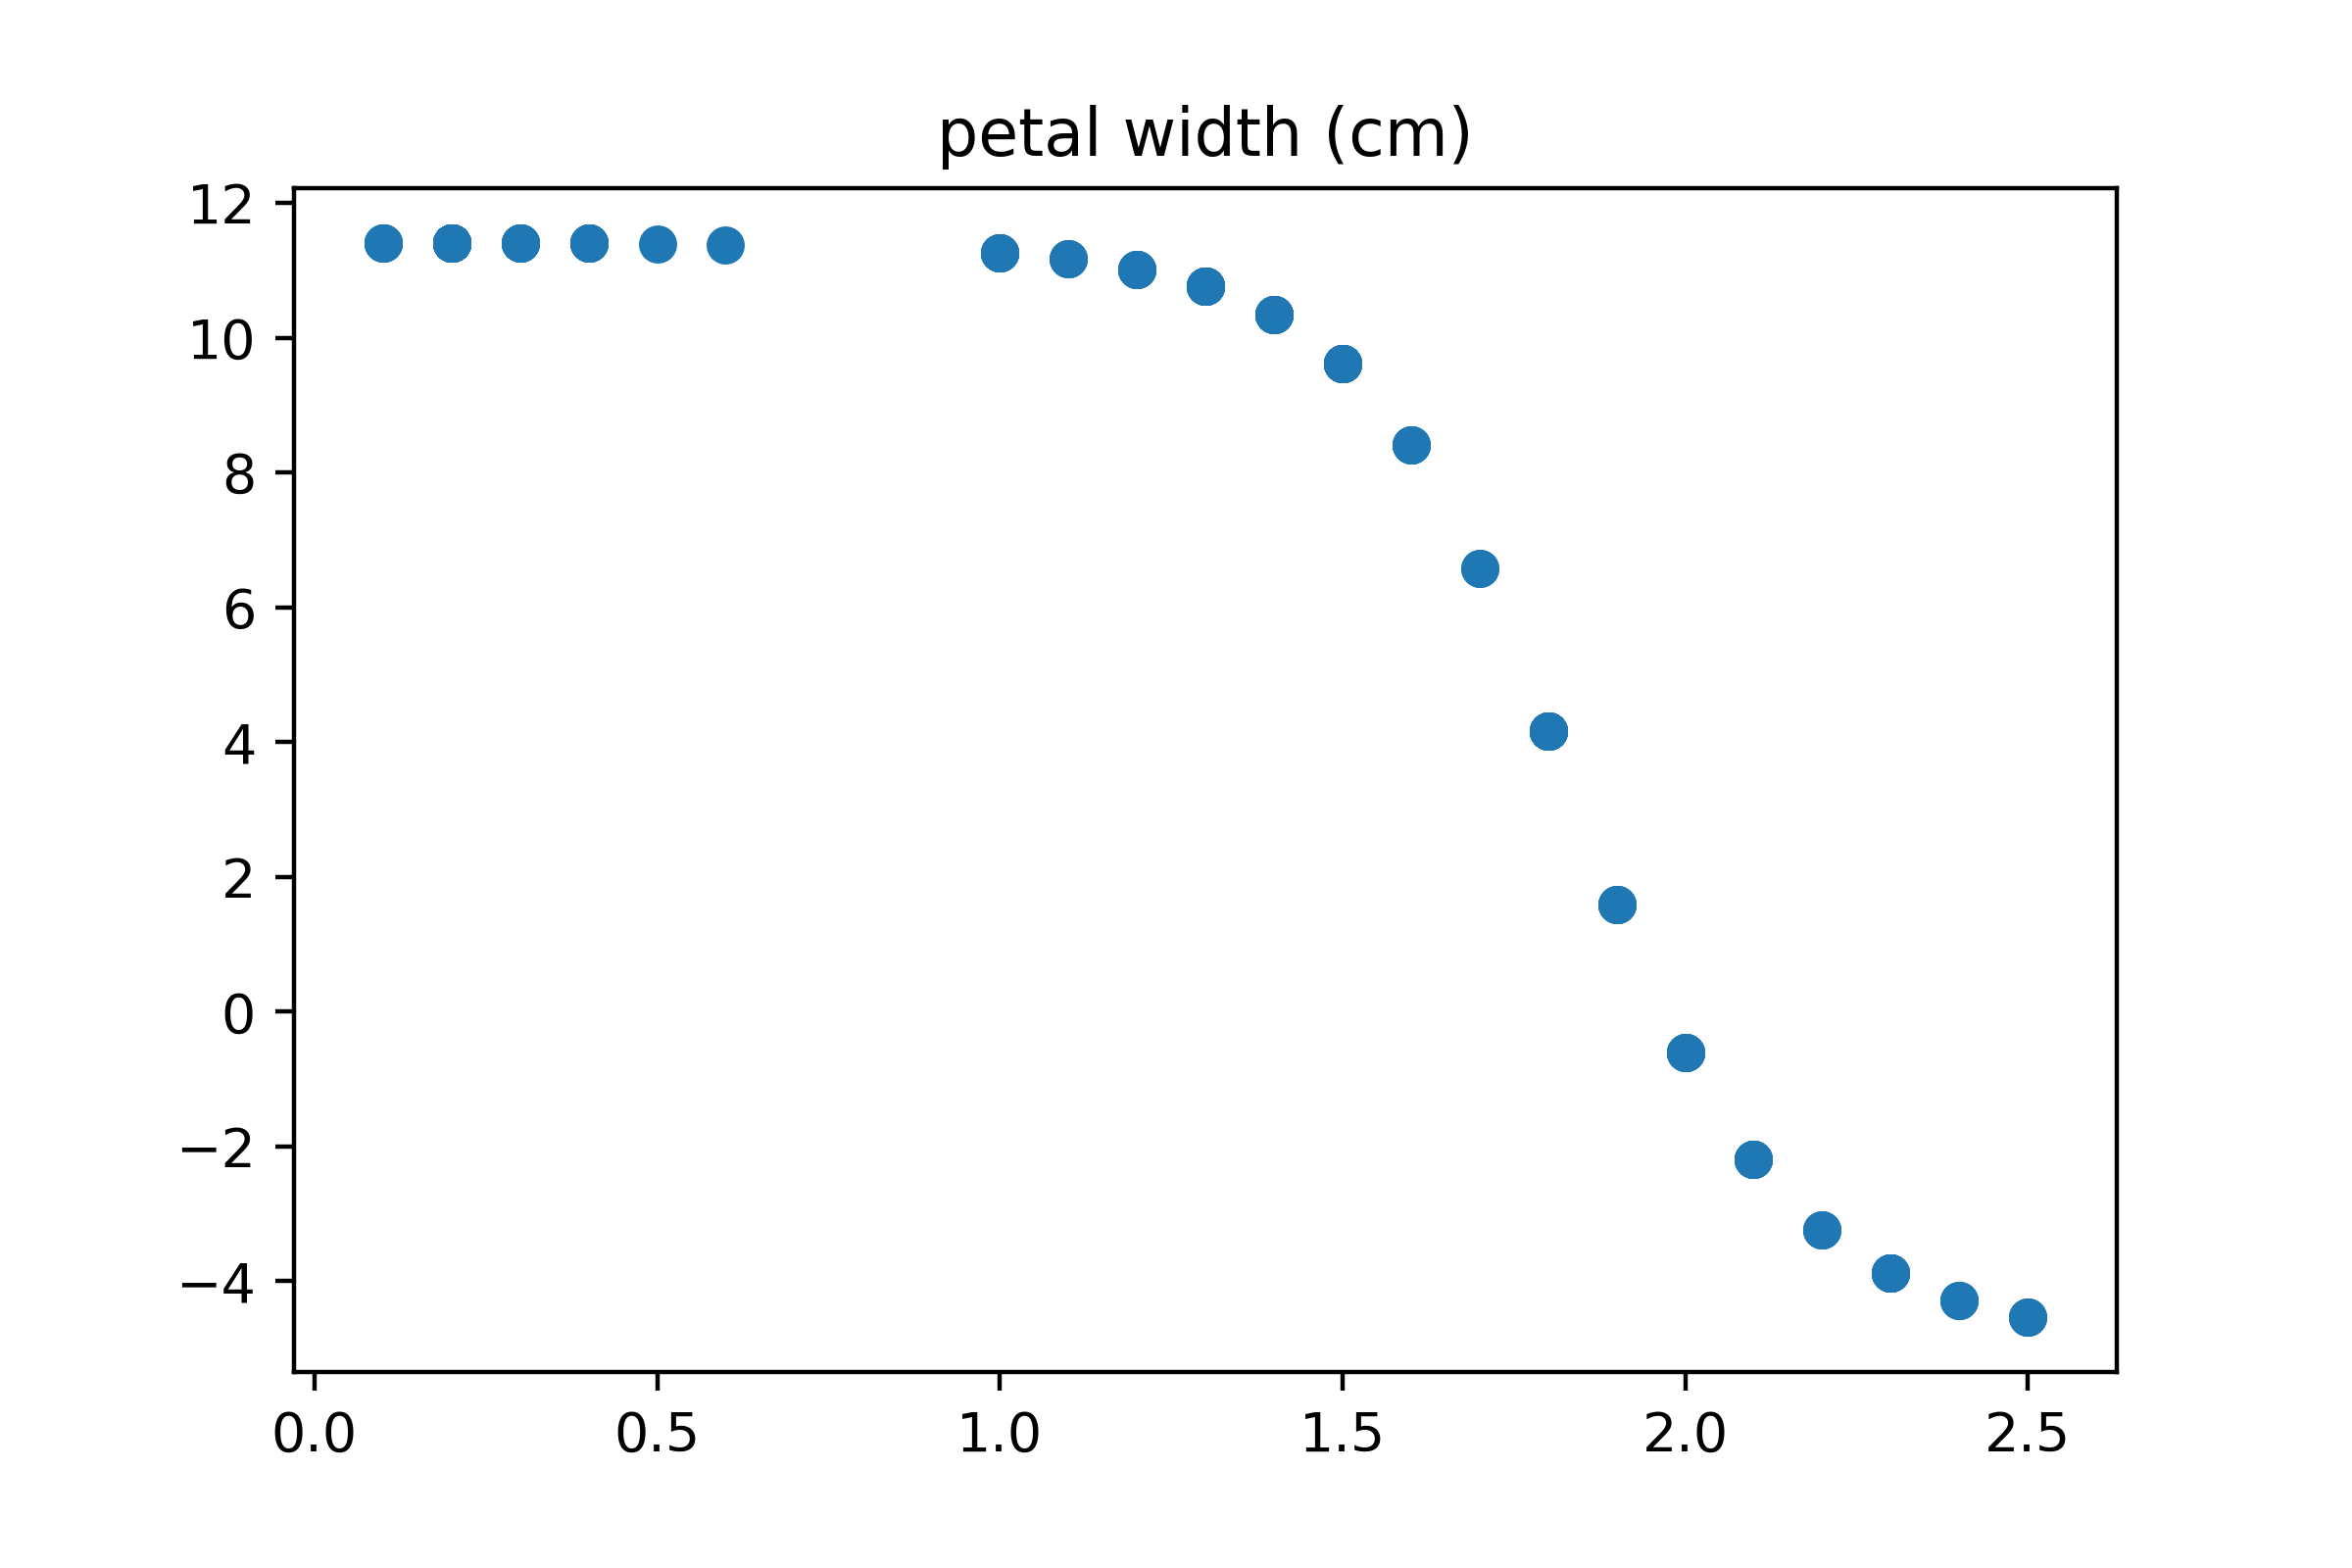
\includegraphics[width=.33\textwidth]{fig/mnl/ir2.png}%
        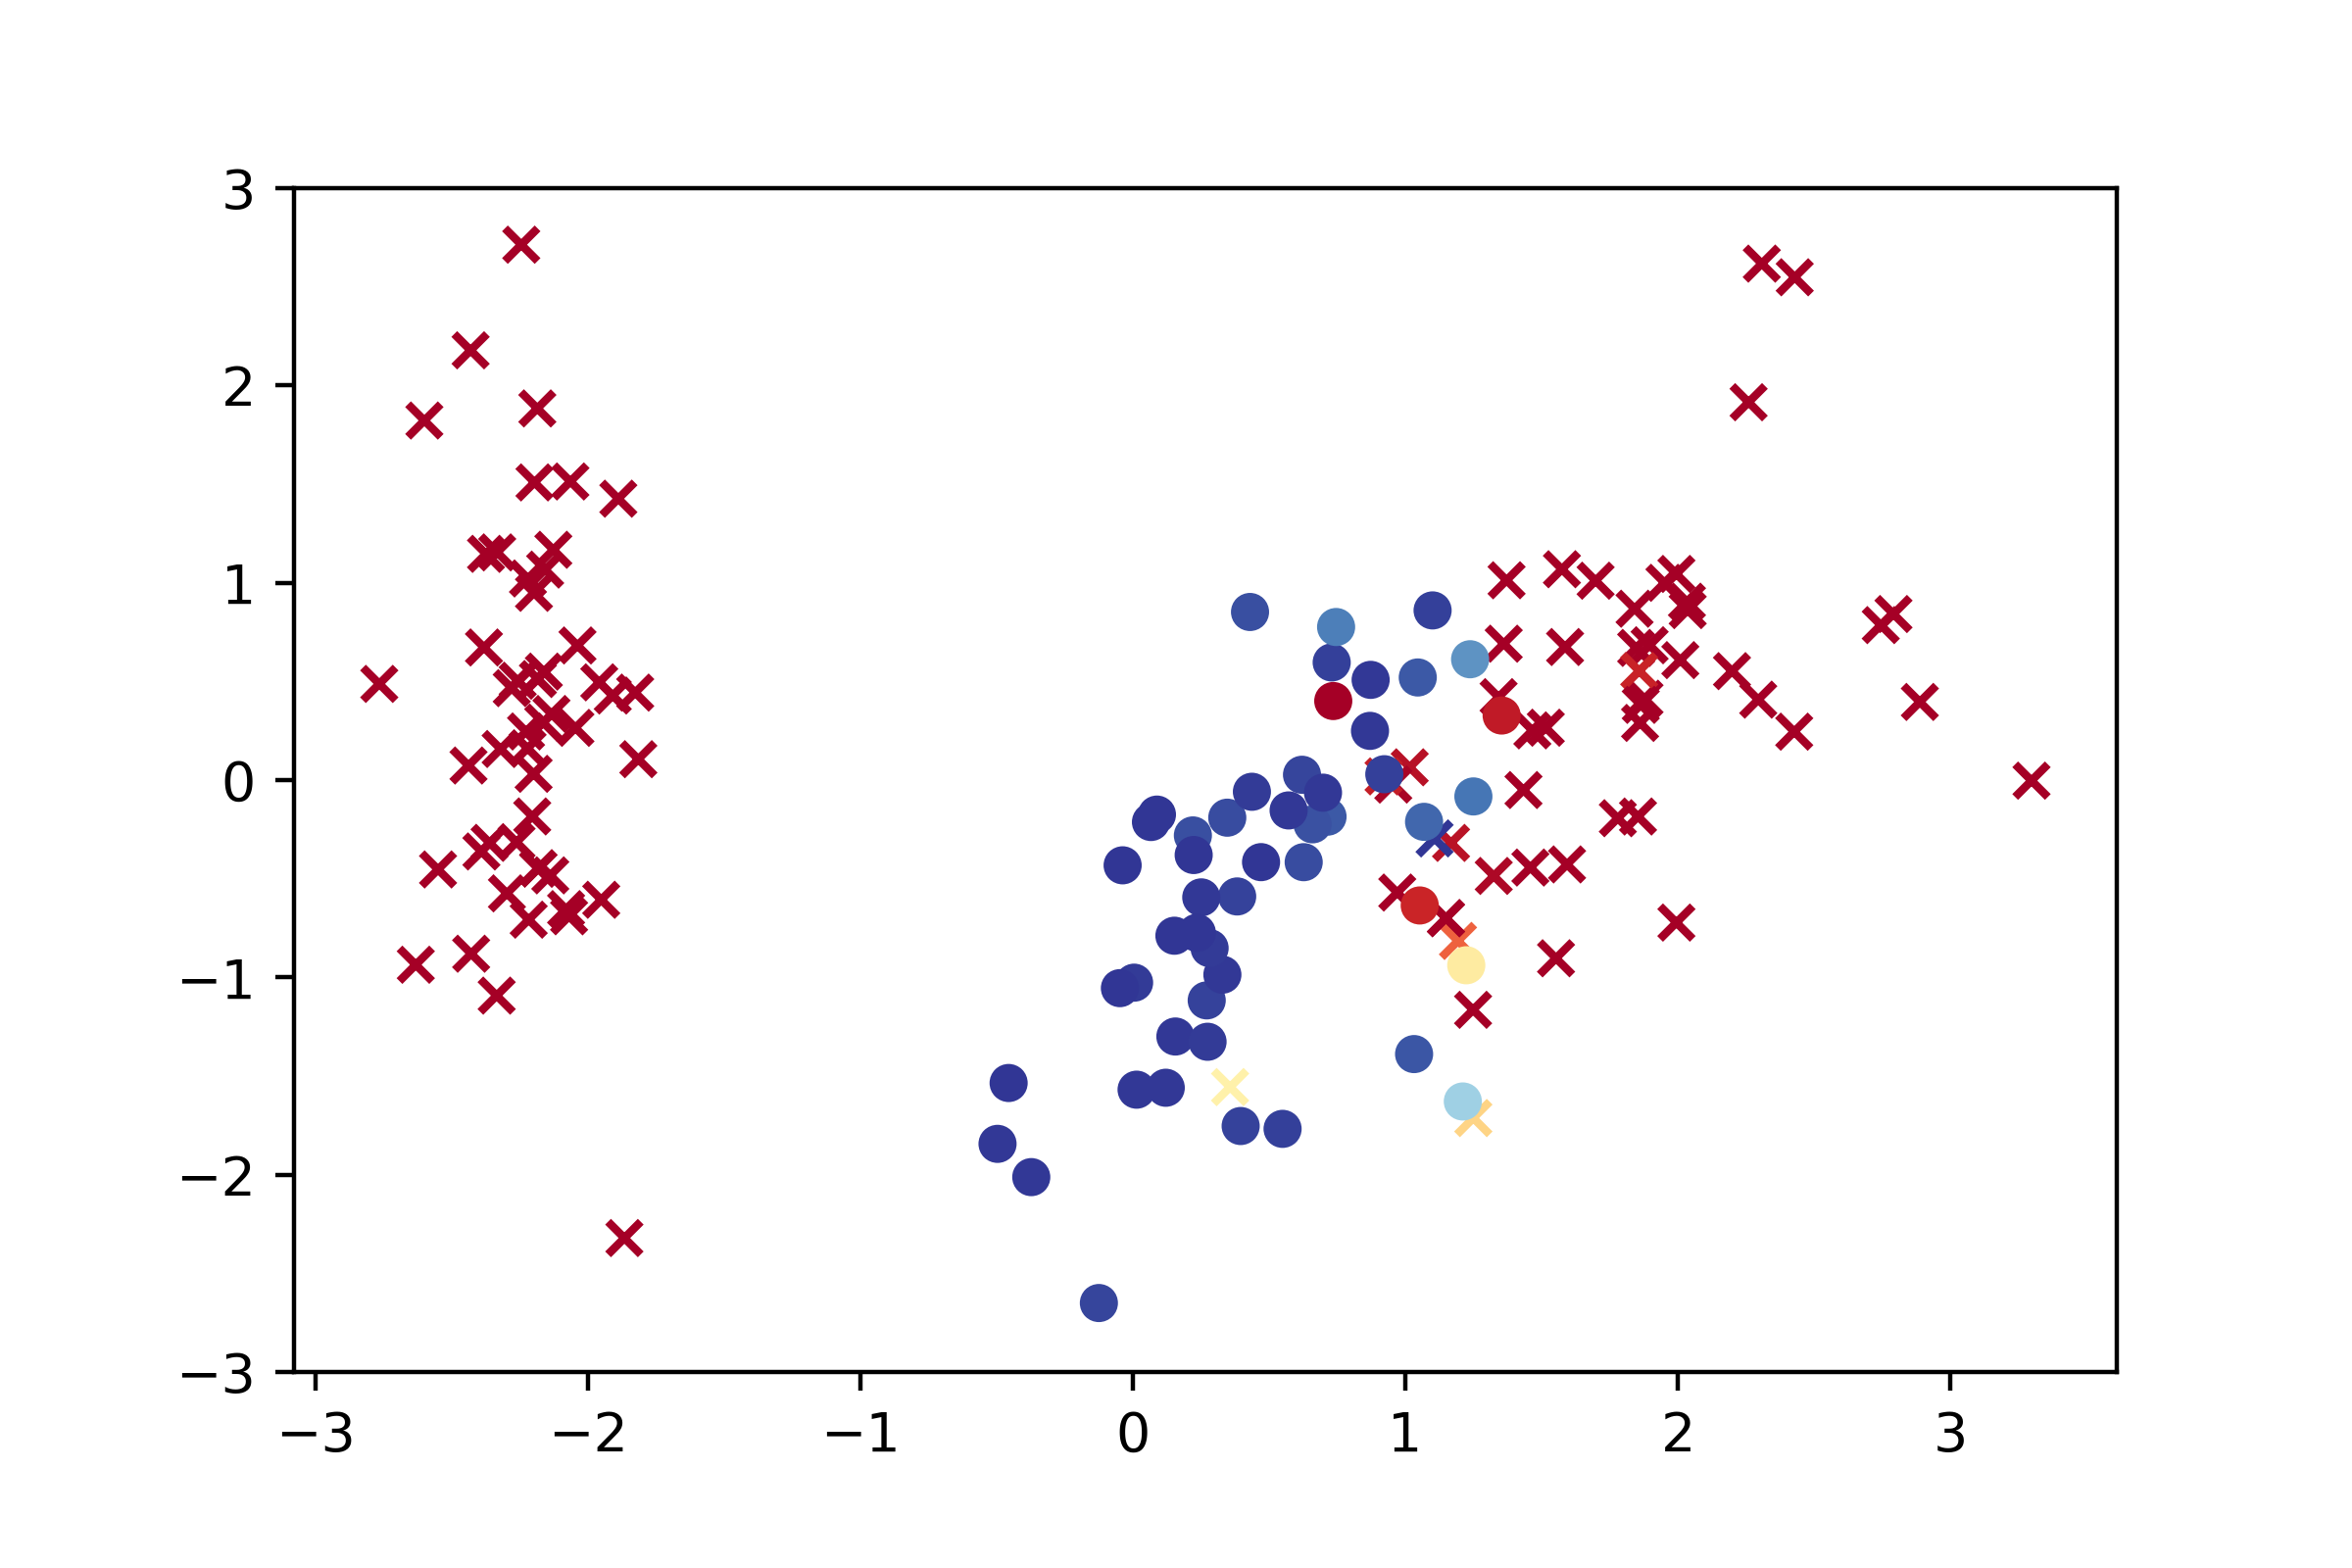
\includegraphics[width=.33\textwidth]{fig/plt/ir.png}
        \caption{Iris Dataset}
    \end{subfigure}
    \begin{subfigure}{1.0\textwidth}
        \centering
        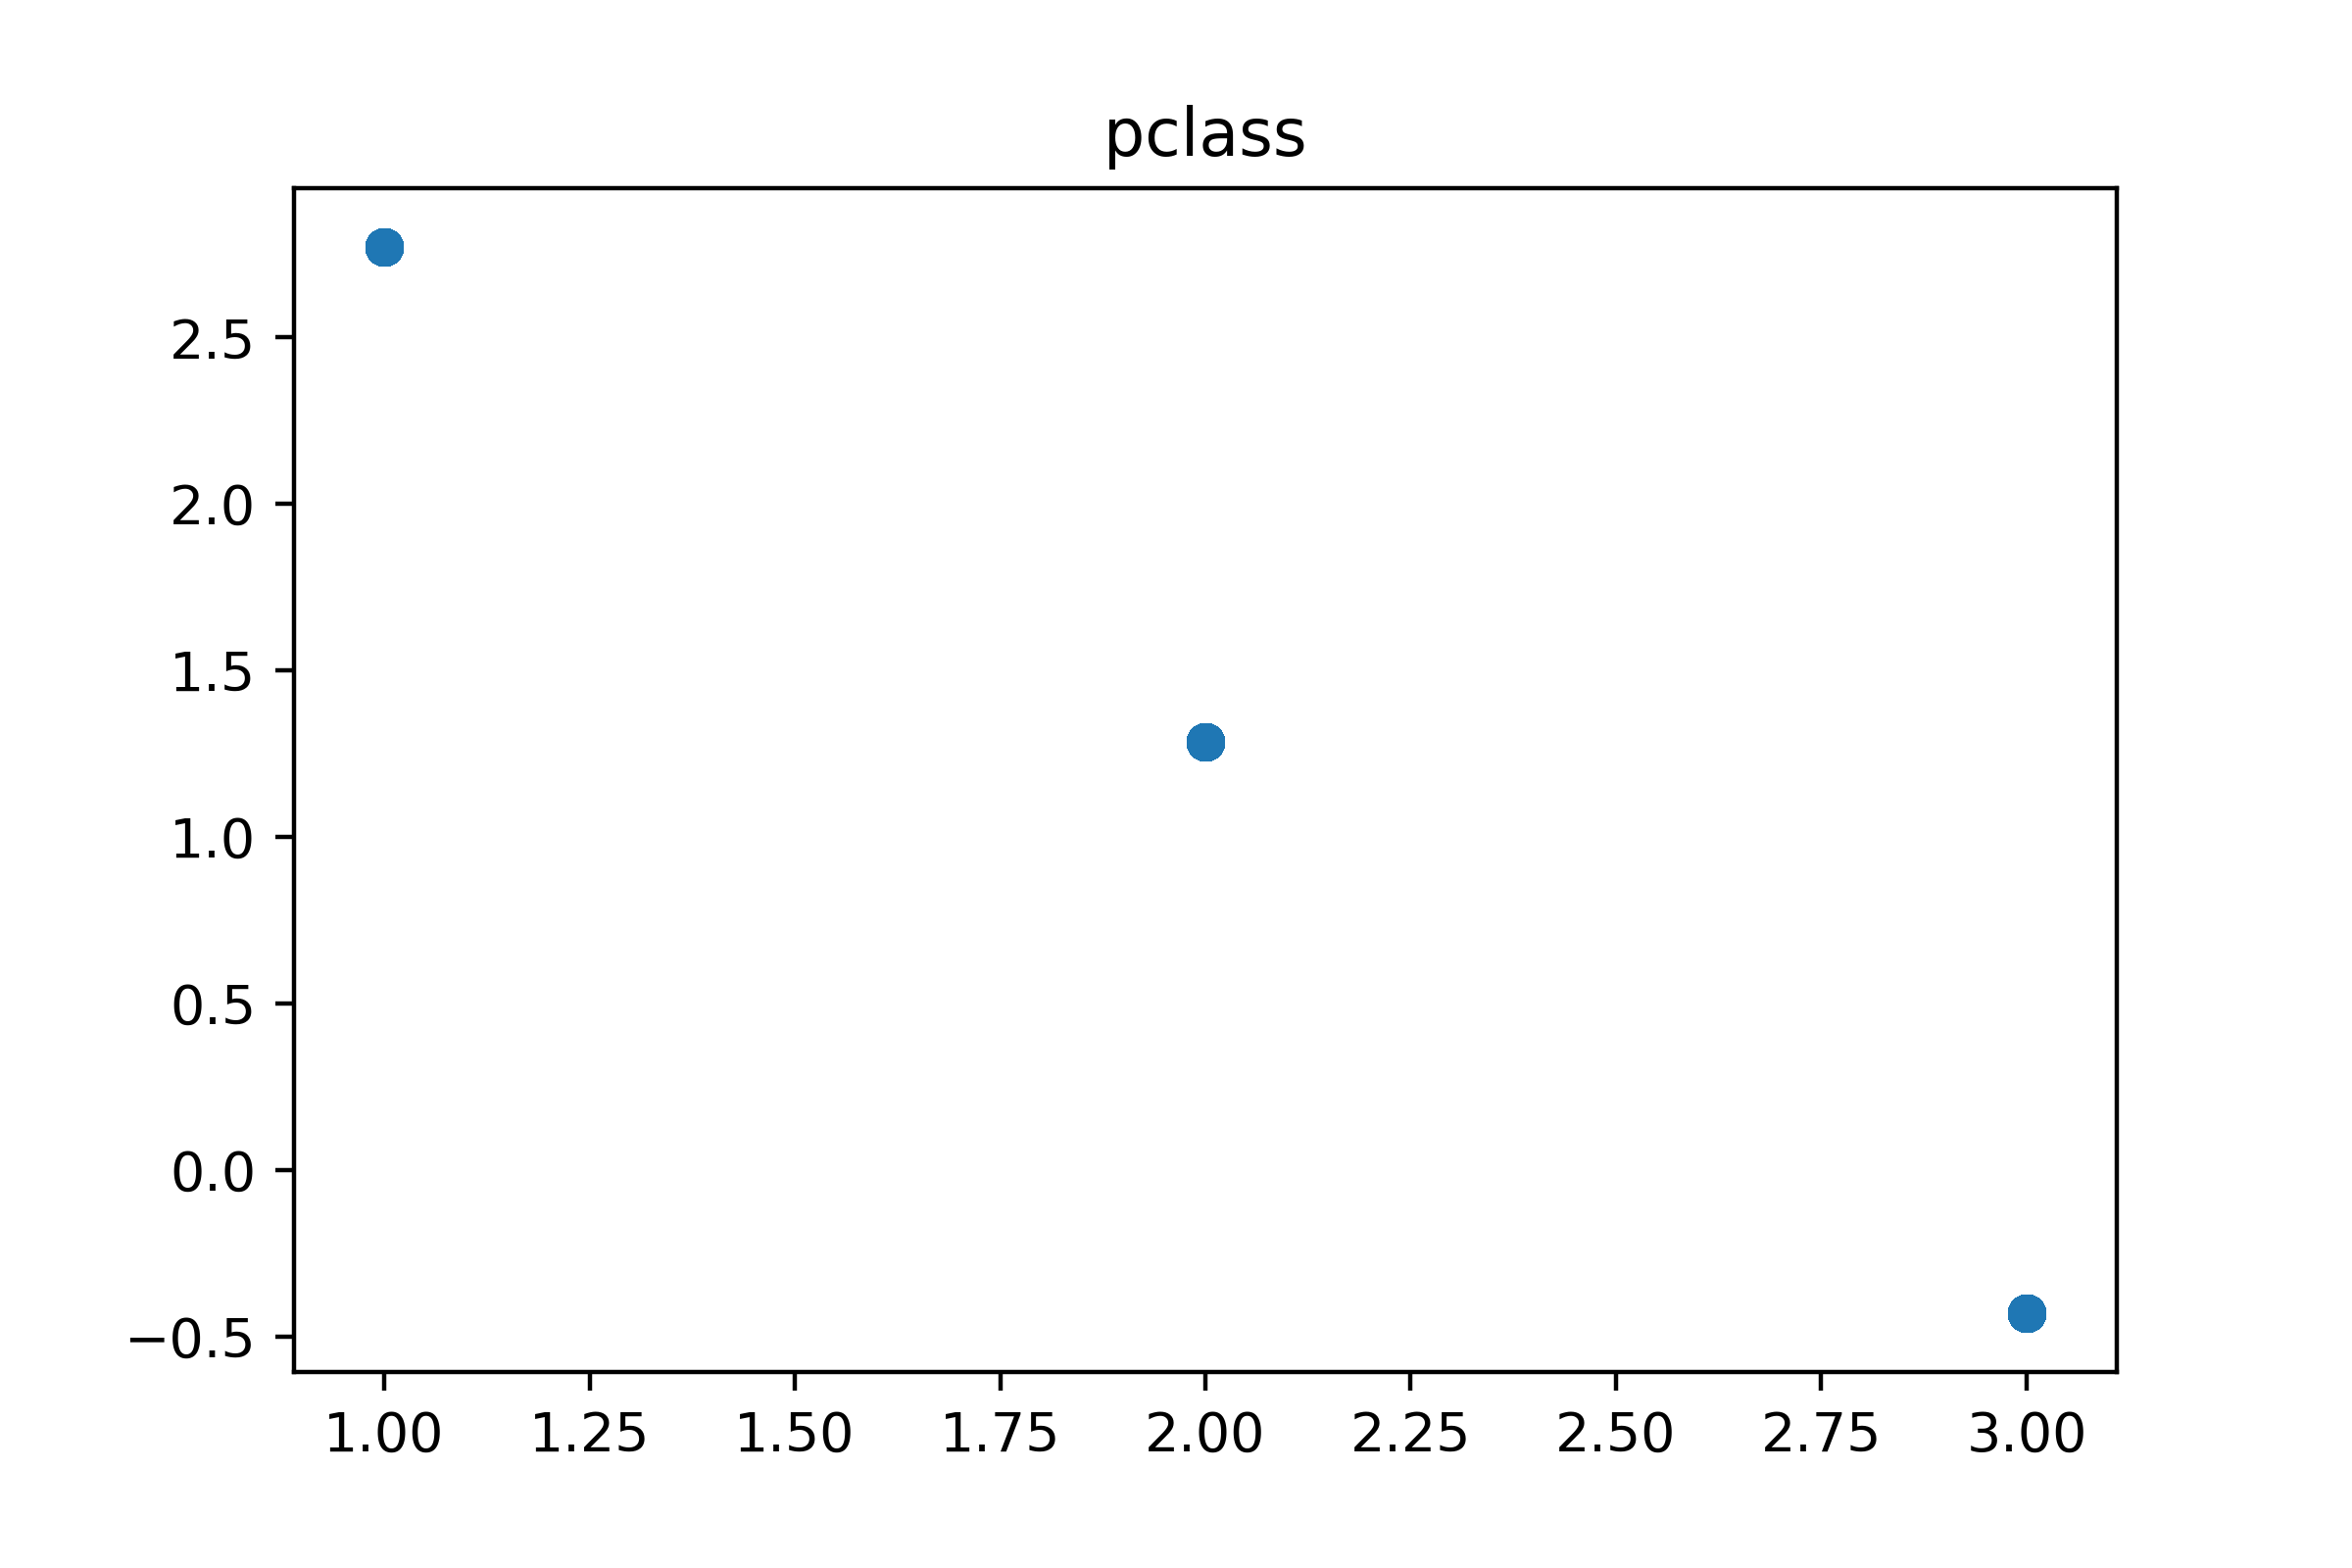
\includegraphics[width=.33\textwidth]{fig/mnl/ti1.png}%
        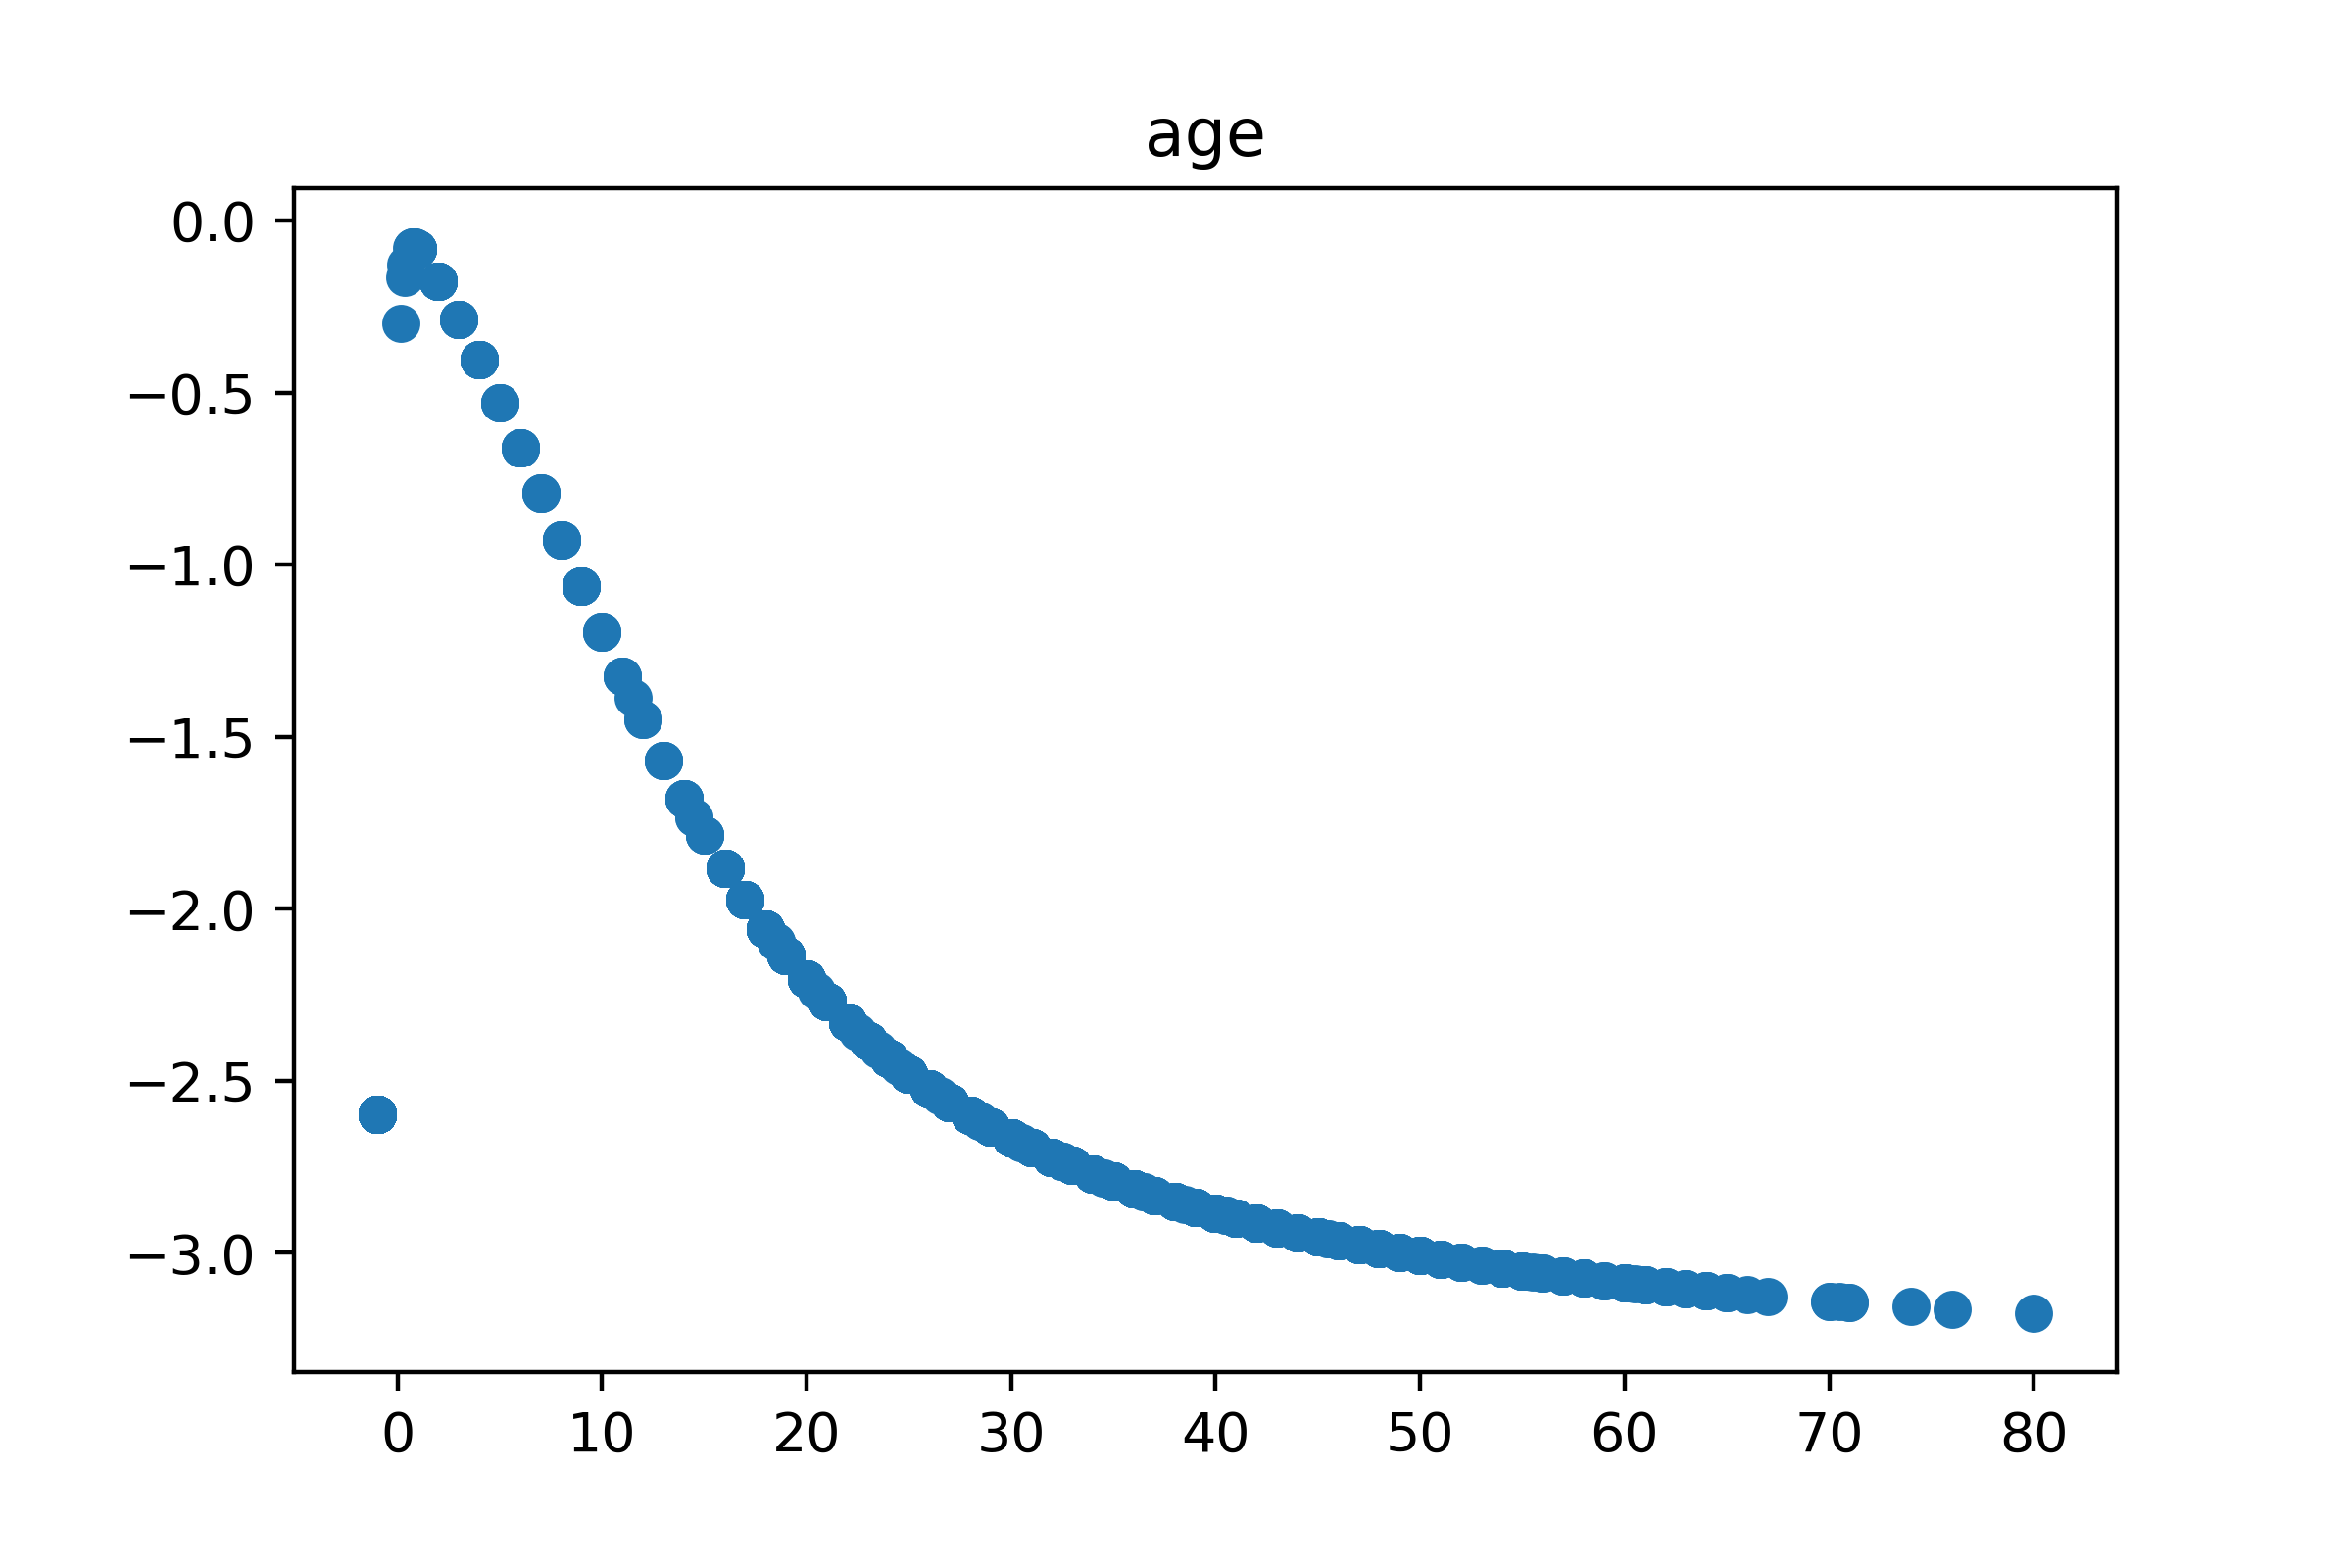
\includegraphics[width=.33\textwidth]{fig/mnl/ti2.png}%
        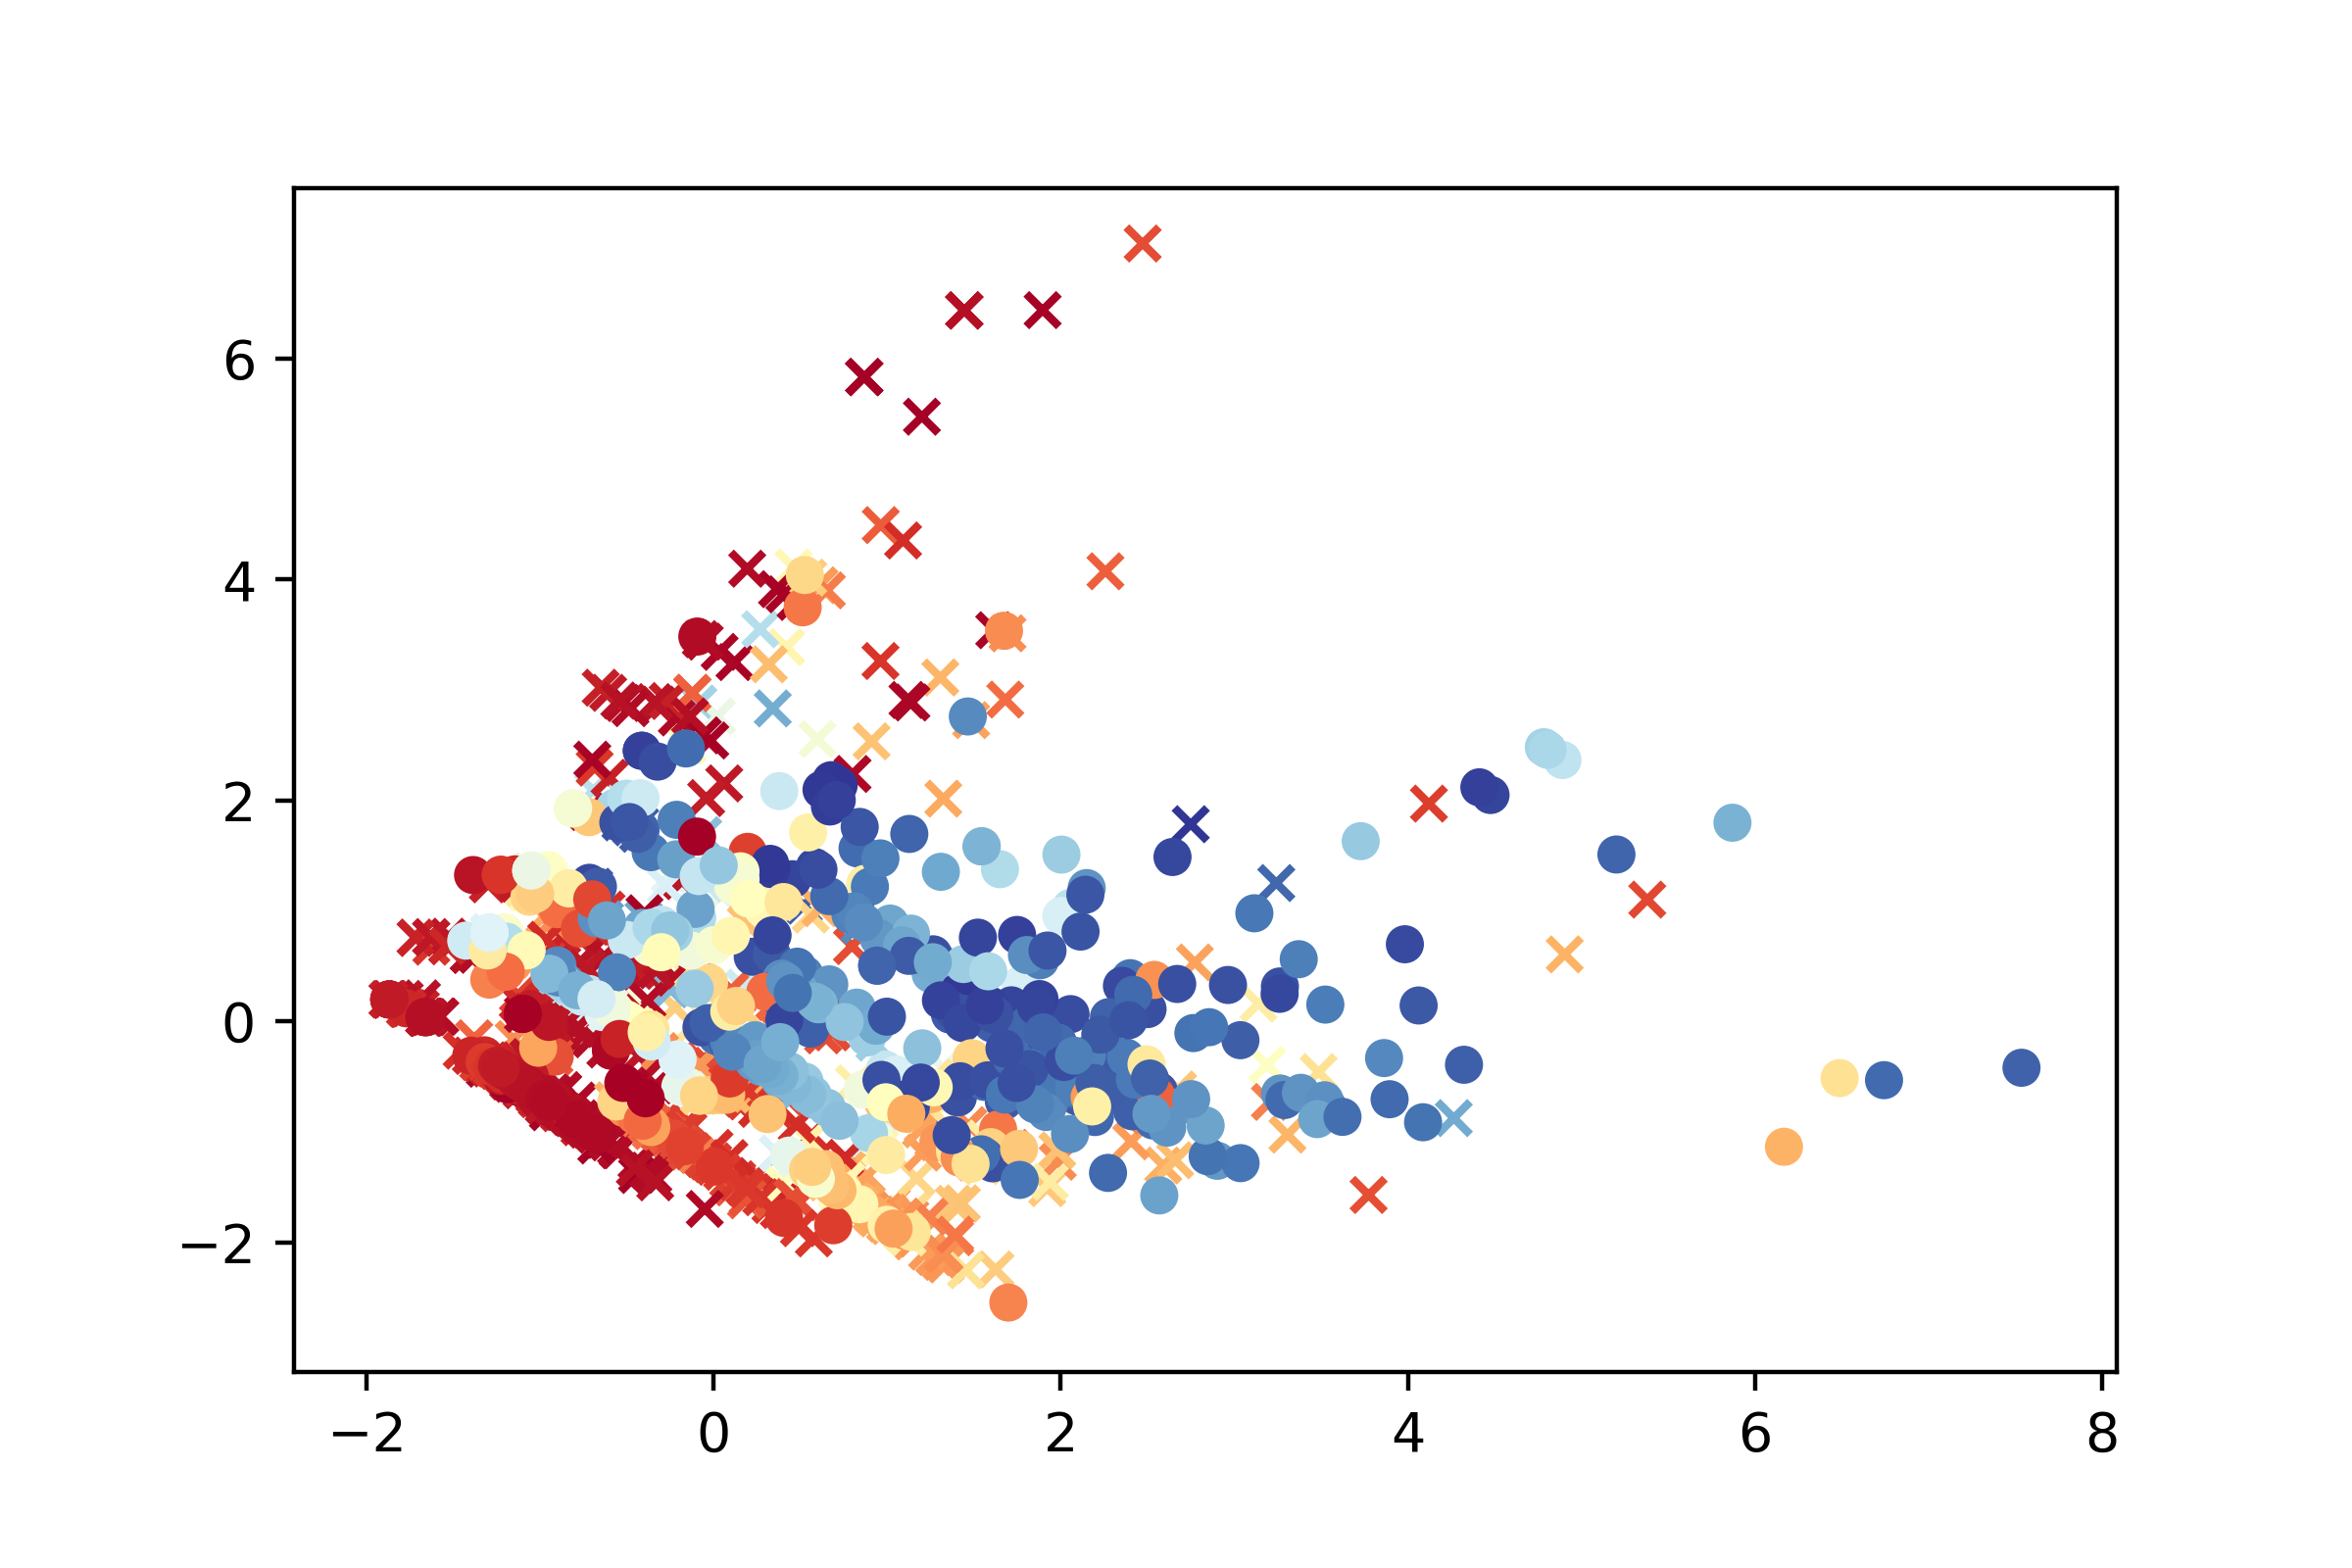
\includegraphics[width=.33\textwidth]{fig/plt/ti.png}
        \caption{Titanic Dataset}
    \end{subfigure}
    \begin{subfigure}{1.0\textwidth}
        \centering
        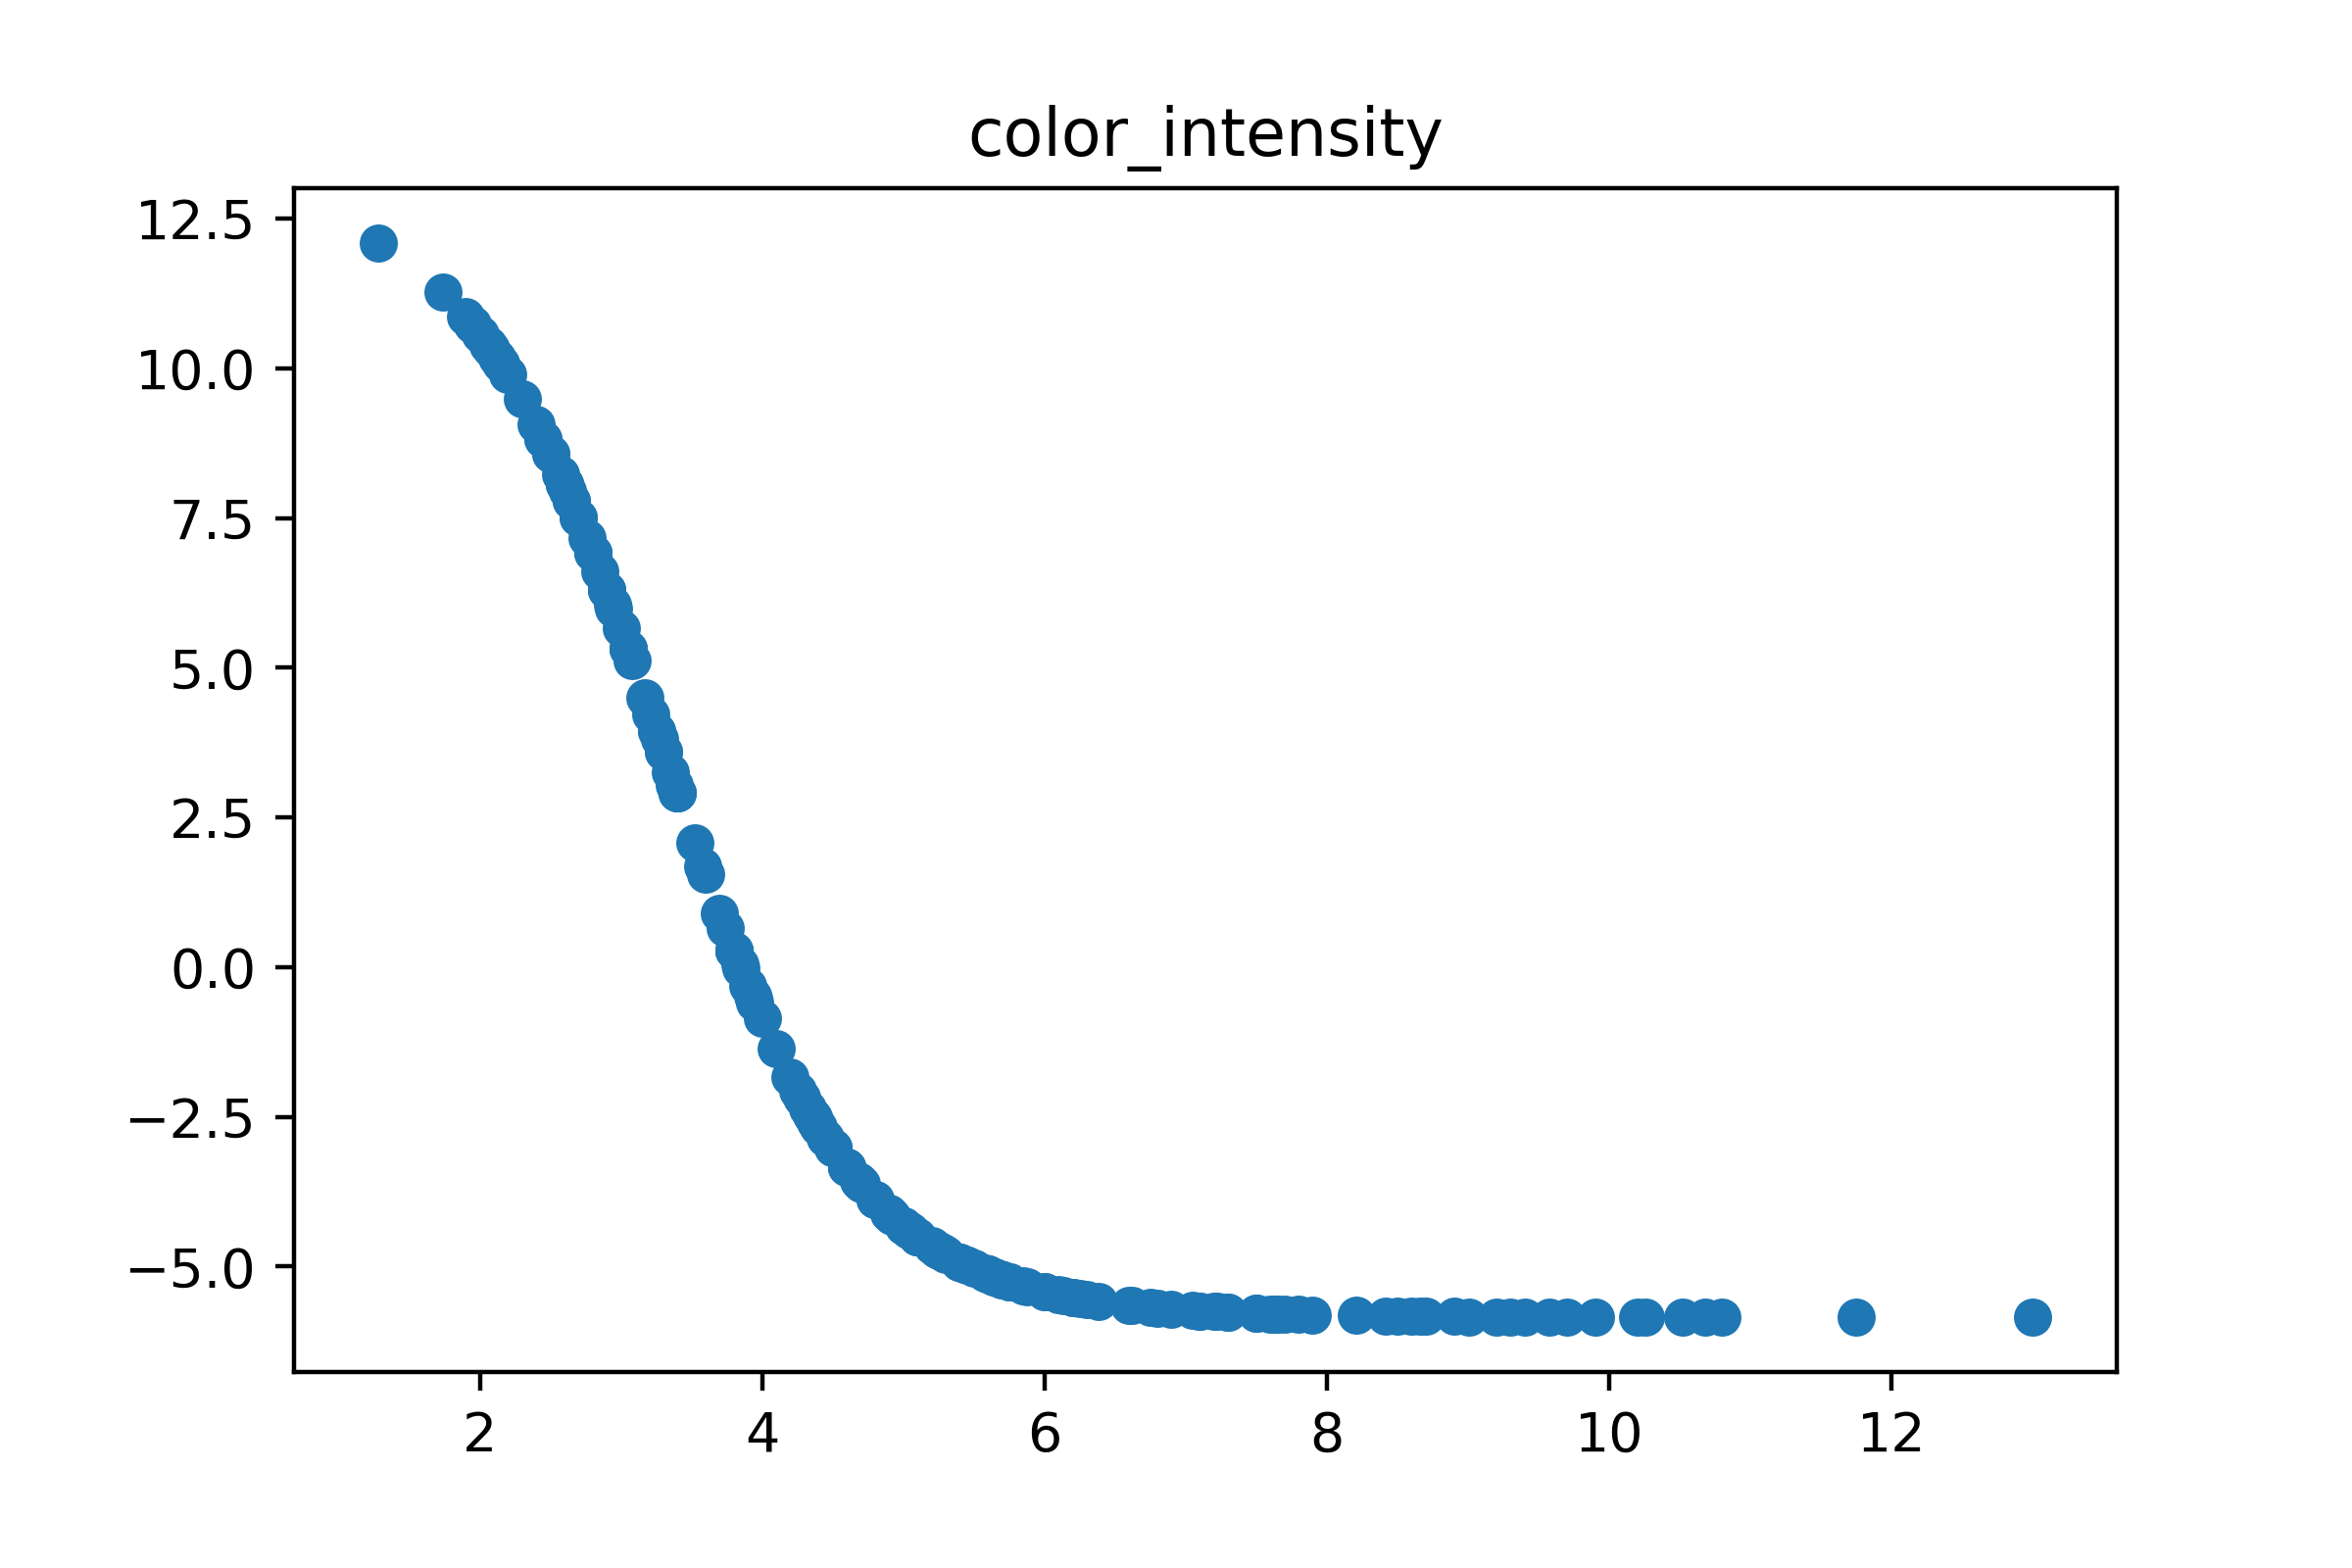
\includegraphics[width=.33\textwidth]{fig/mnl/wi1.png}%
        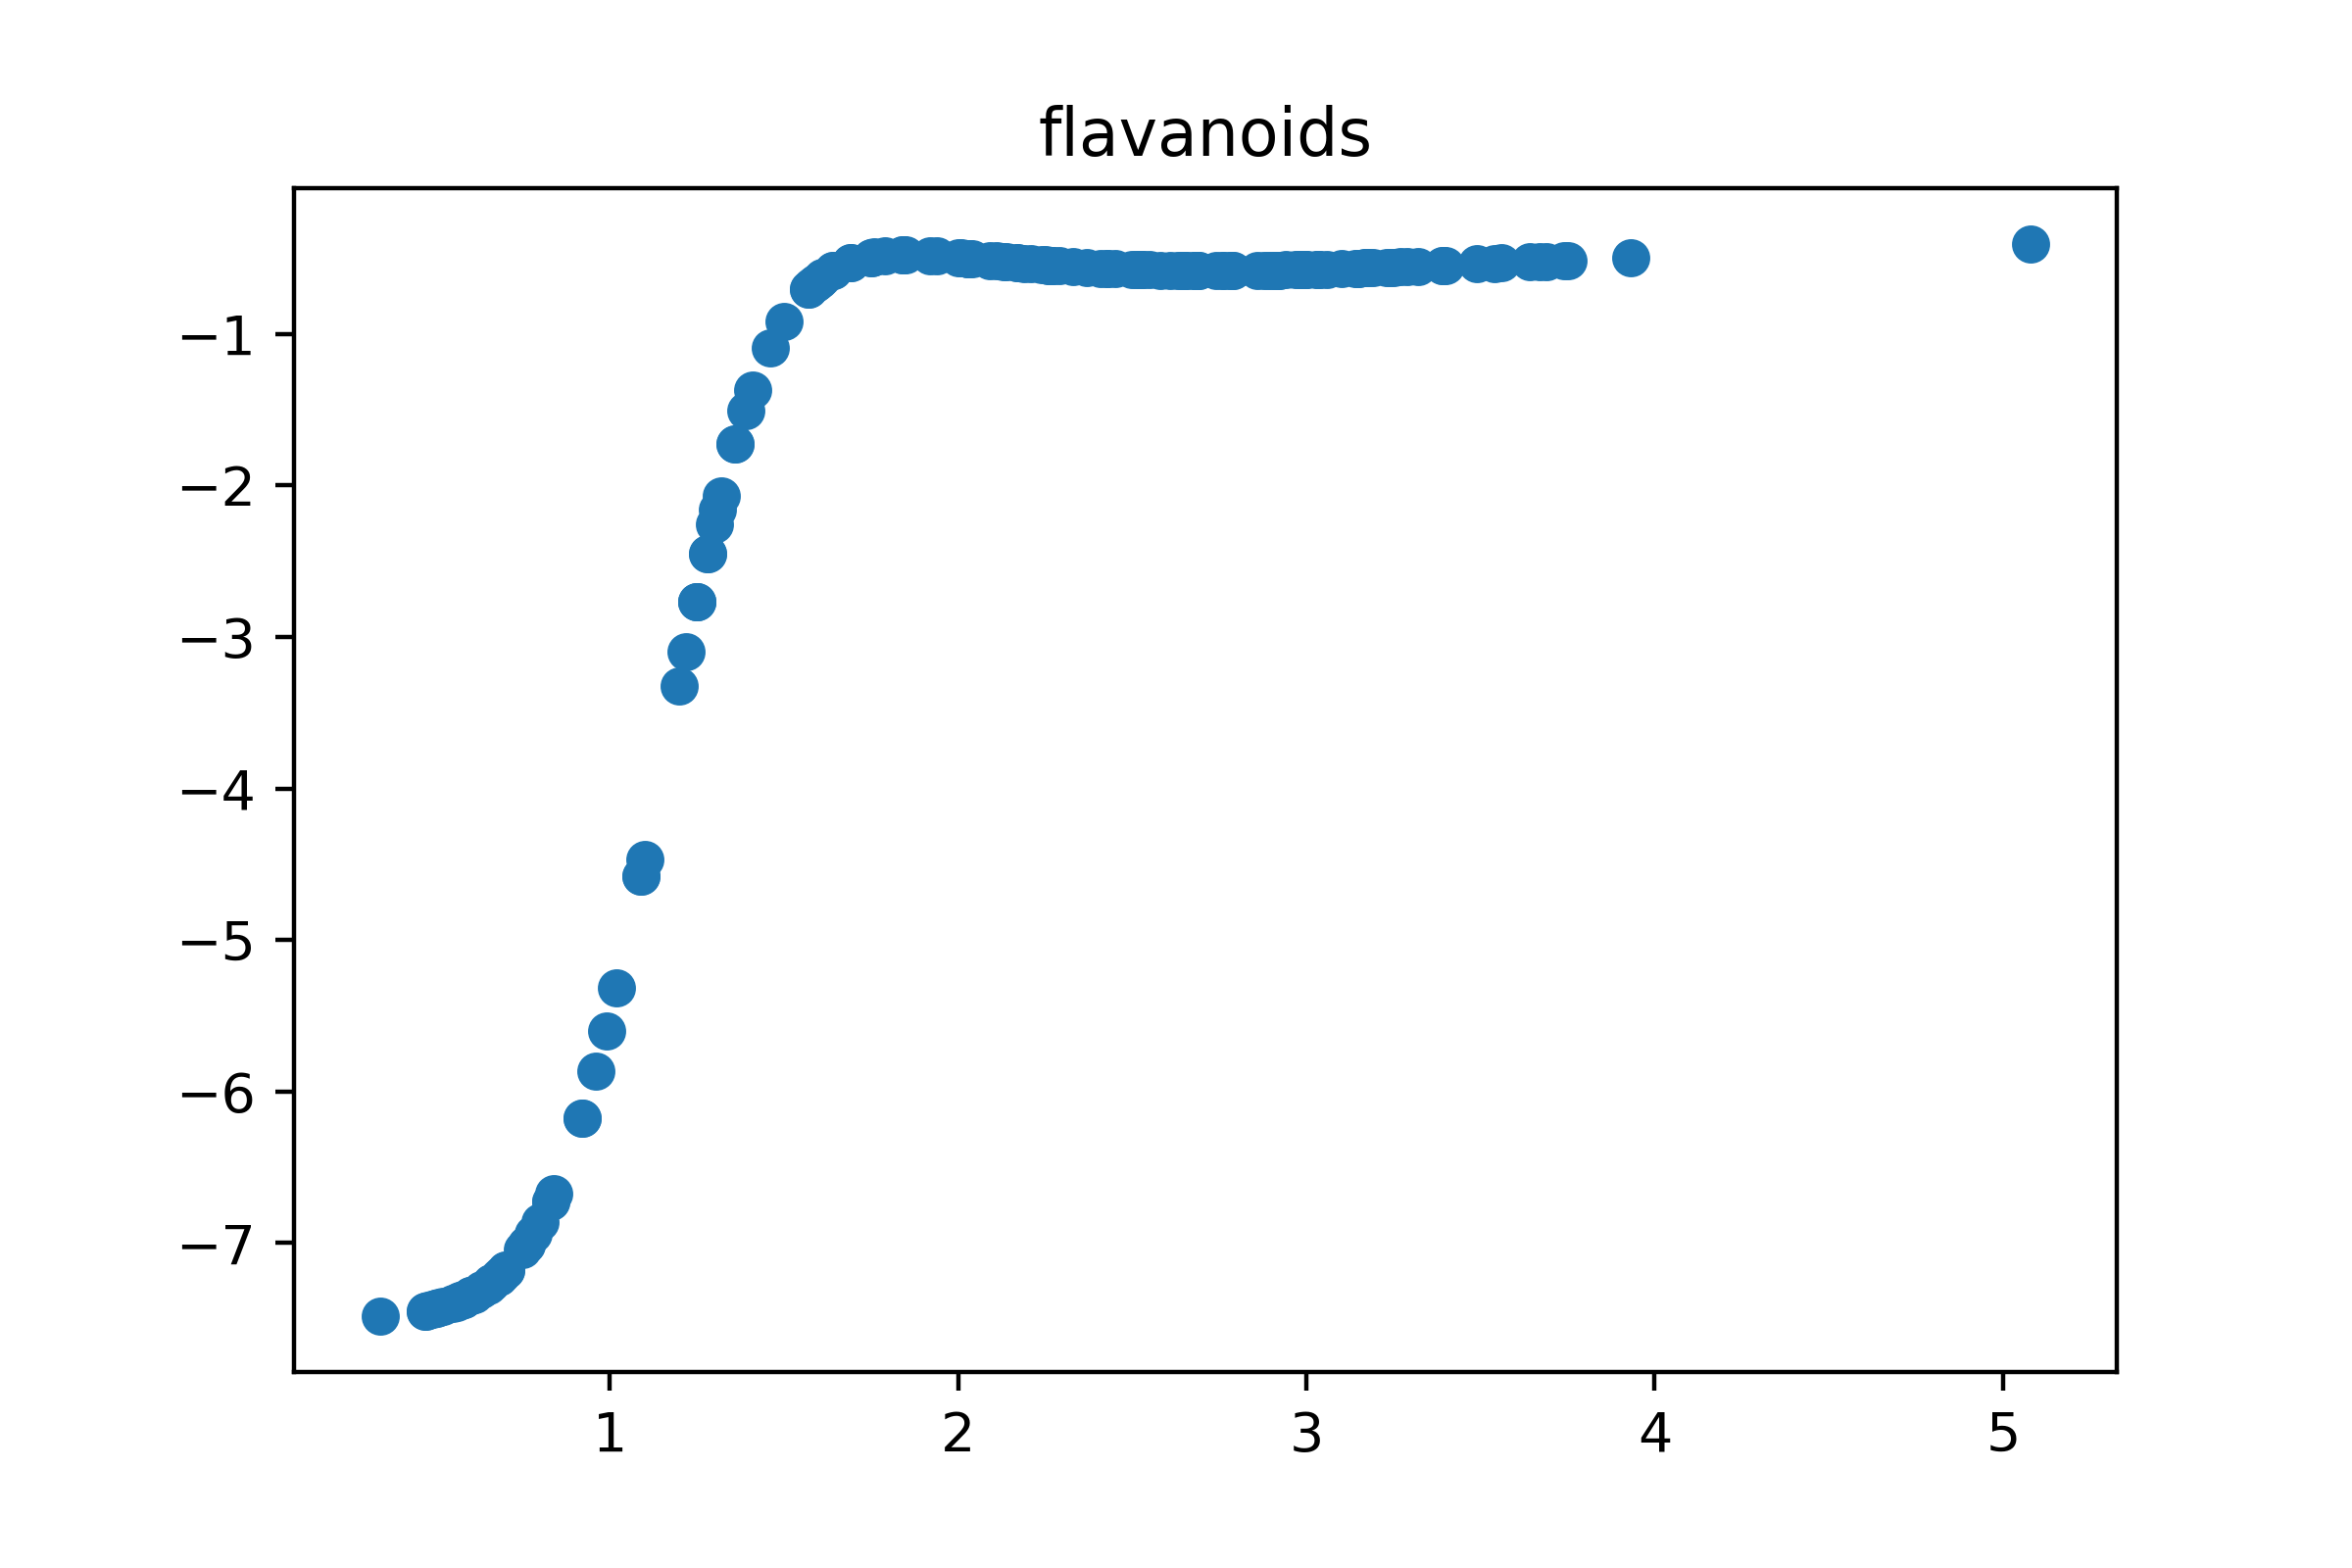
\includegraphics[width=.33\textwidth]{fig/mnl/wi2.png}%
        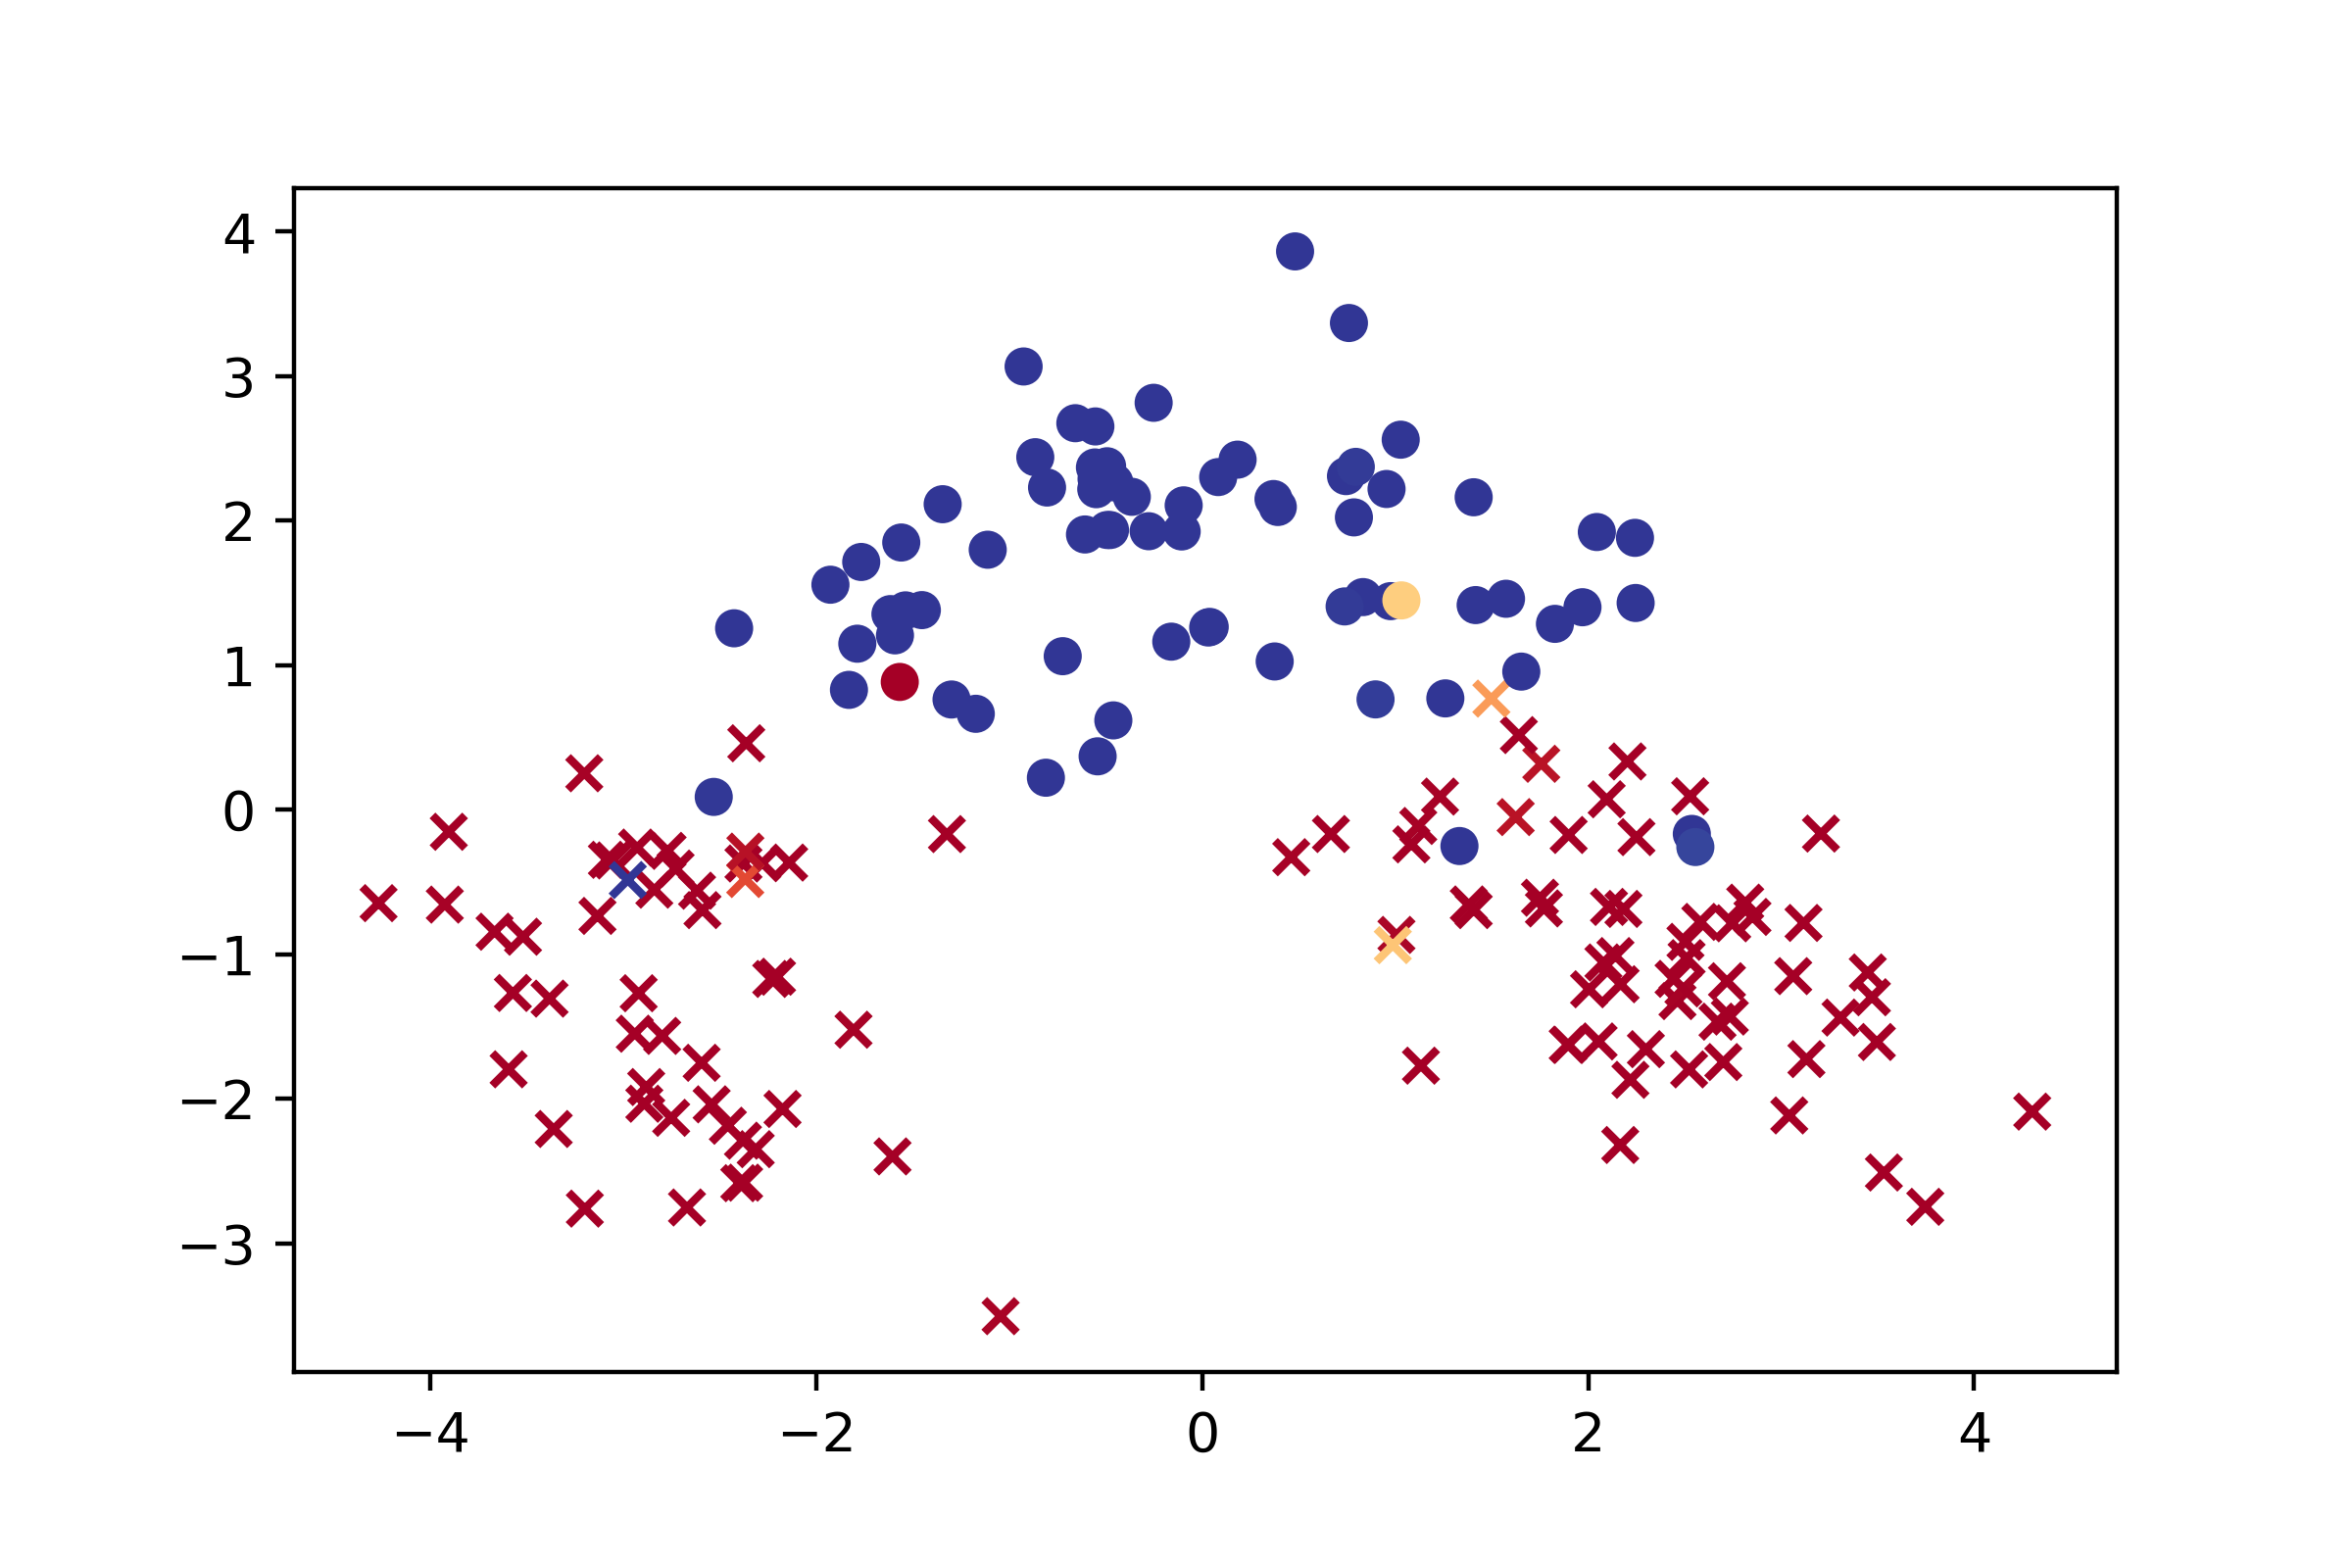
\includegraphics[width=.33\textwidth]{fig/plt/wi.png}
        \caption{Wine Dataset}
    \end{subfigure}
    \caption{Network predictions and selection of marginals for each dataset. For a full explanation, see figure \ref{fig:big_fig_1}.}
\end{figure}


% \begin{longtable}[]{@{}lc@{}}

%     \toprule
%     Dataset & PCA Plot%
%     \tabularnewline
%     \midrule
%     \endhead

%     Cancer &
%     %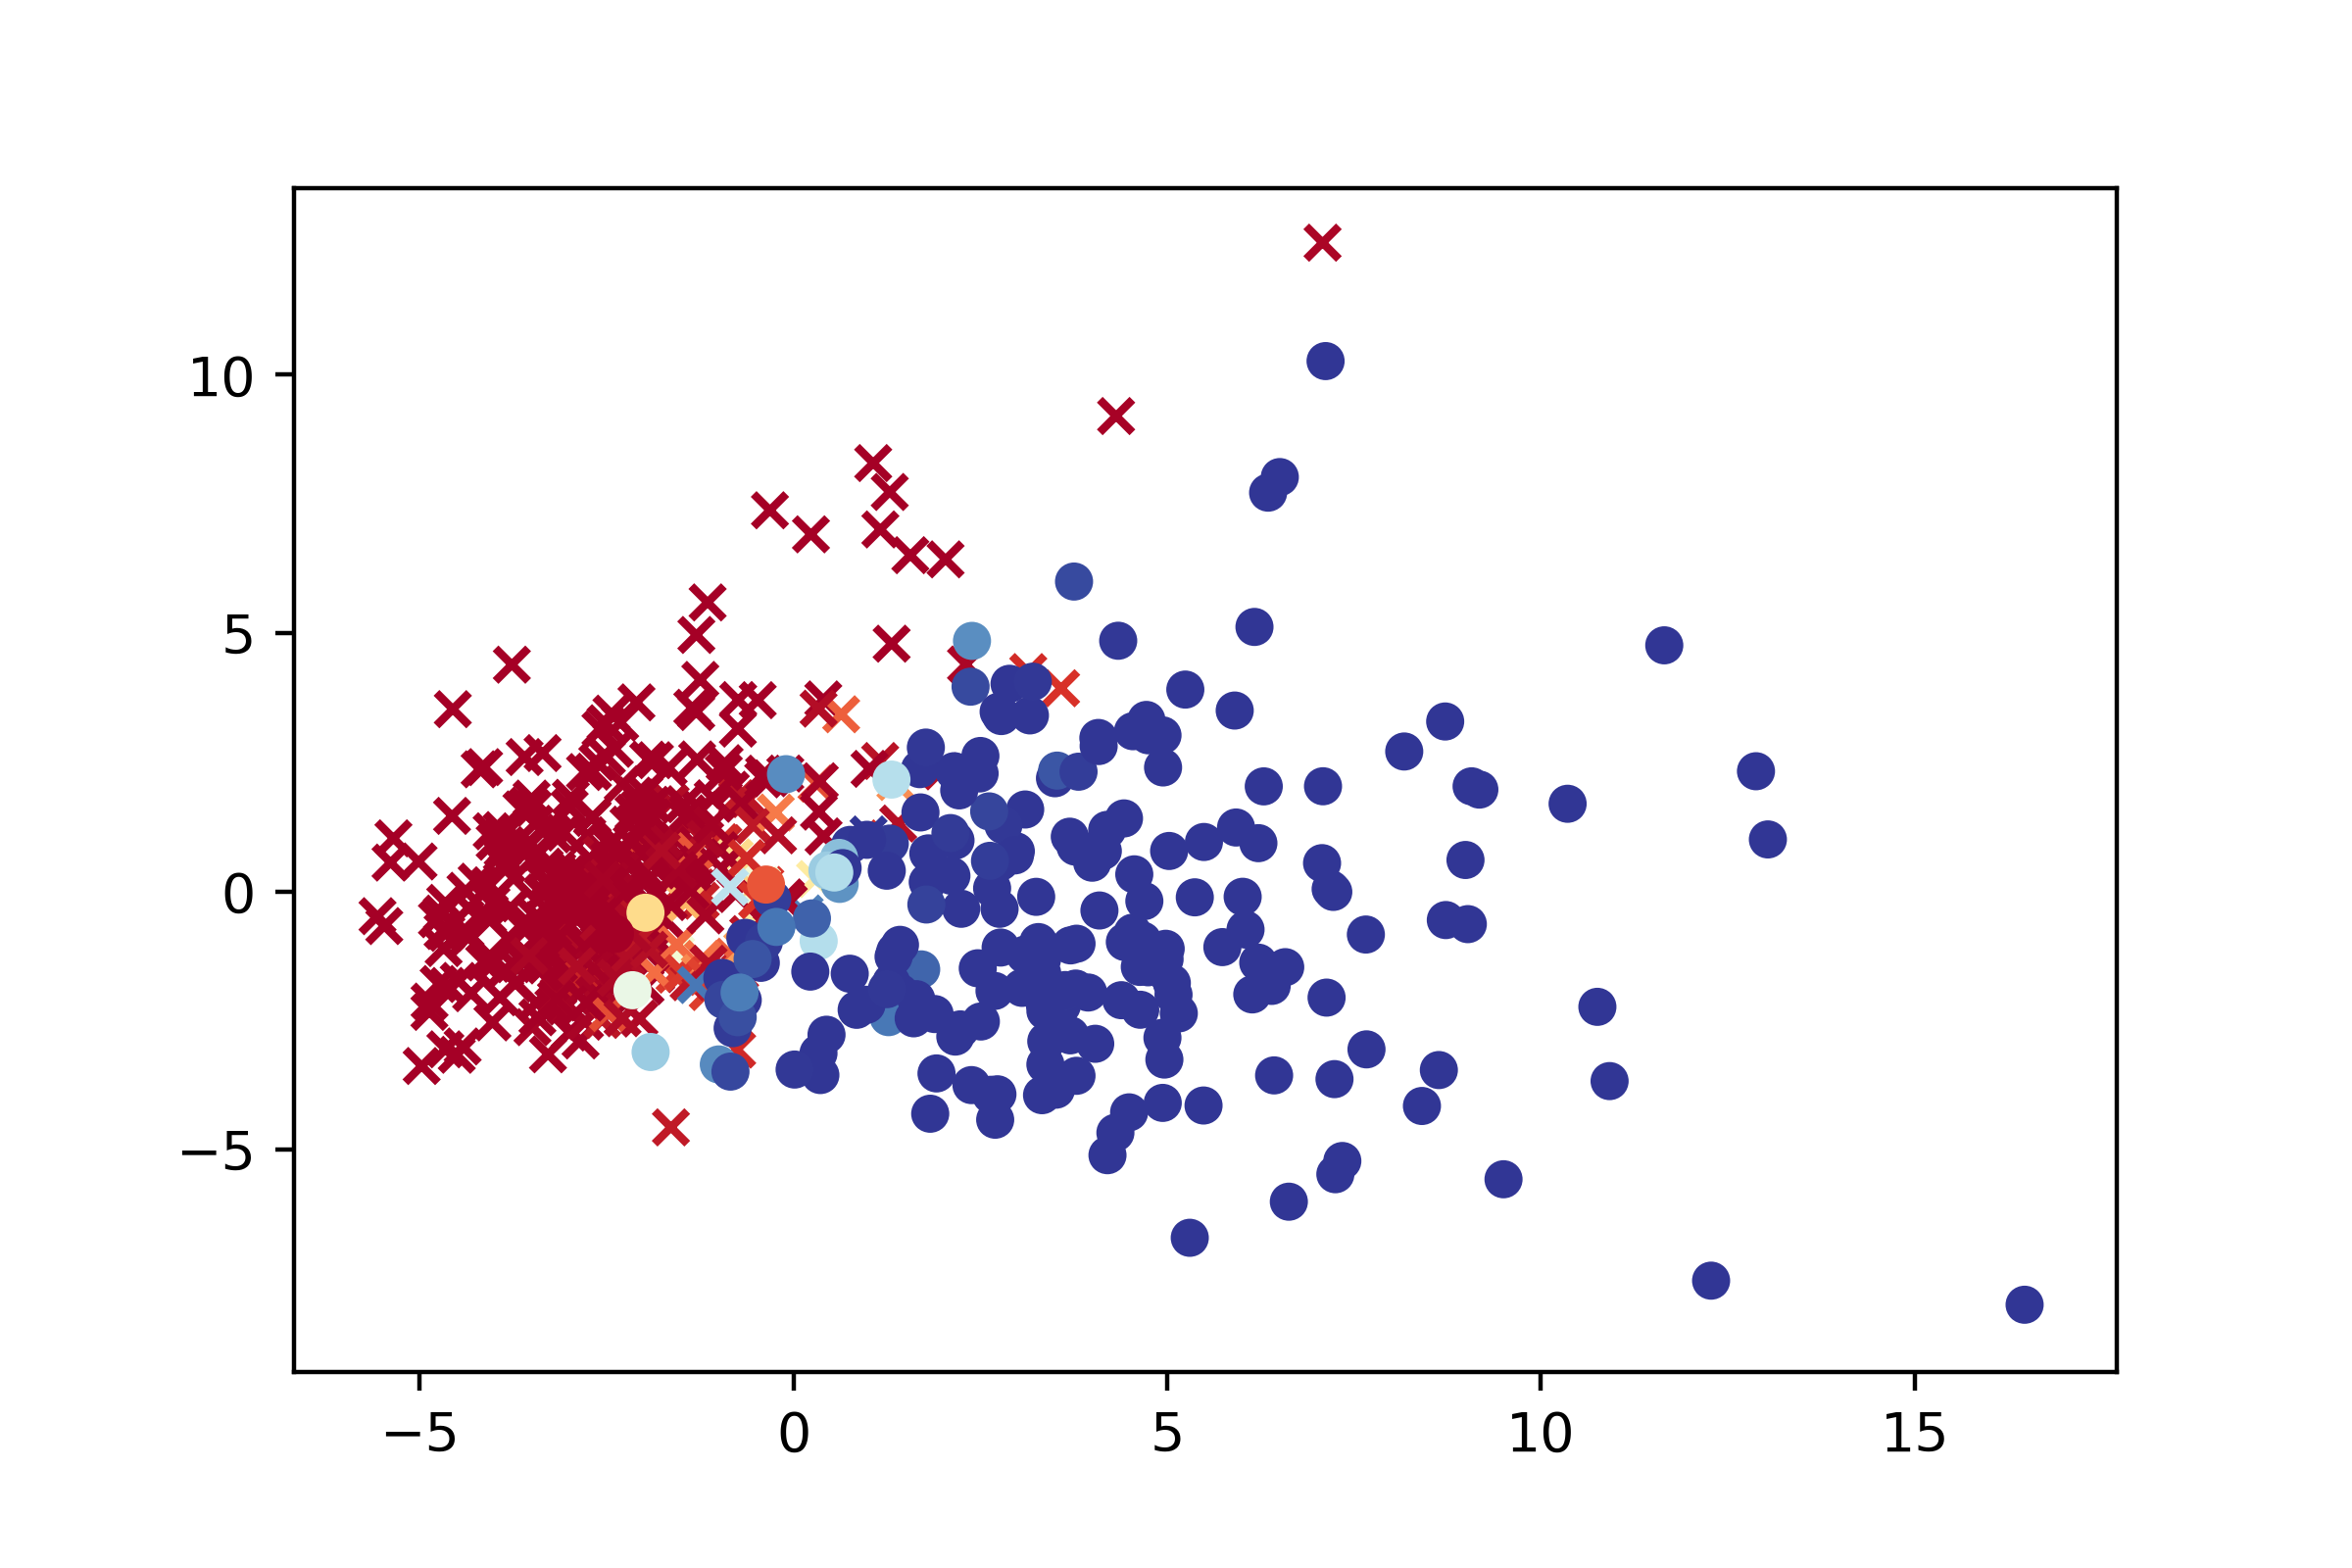
\includegraphics[width=0.22\textwidth]{fig/plt/bc.png} &
%     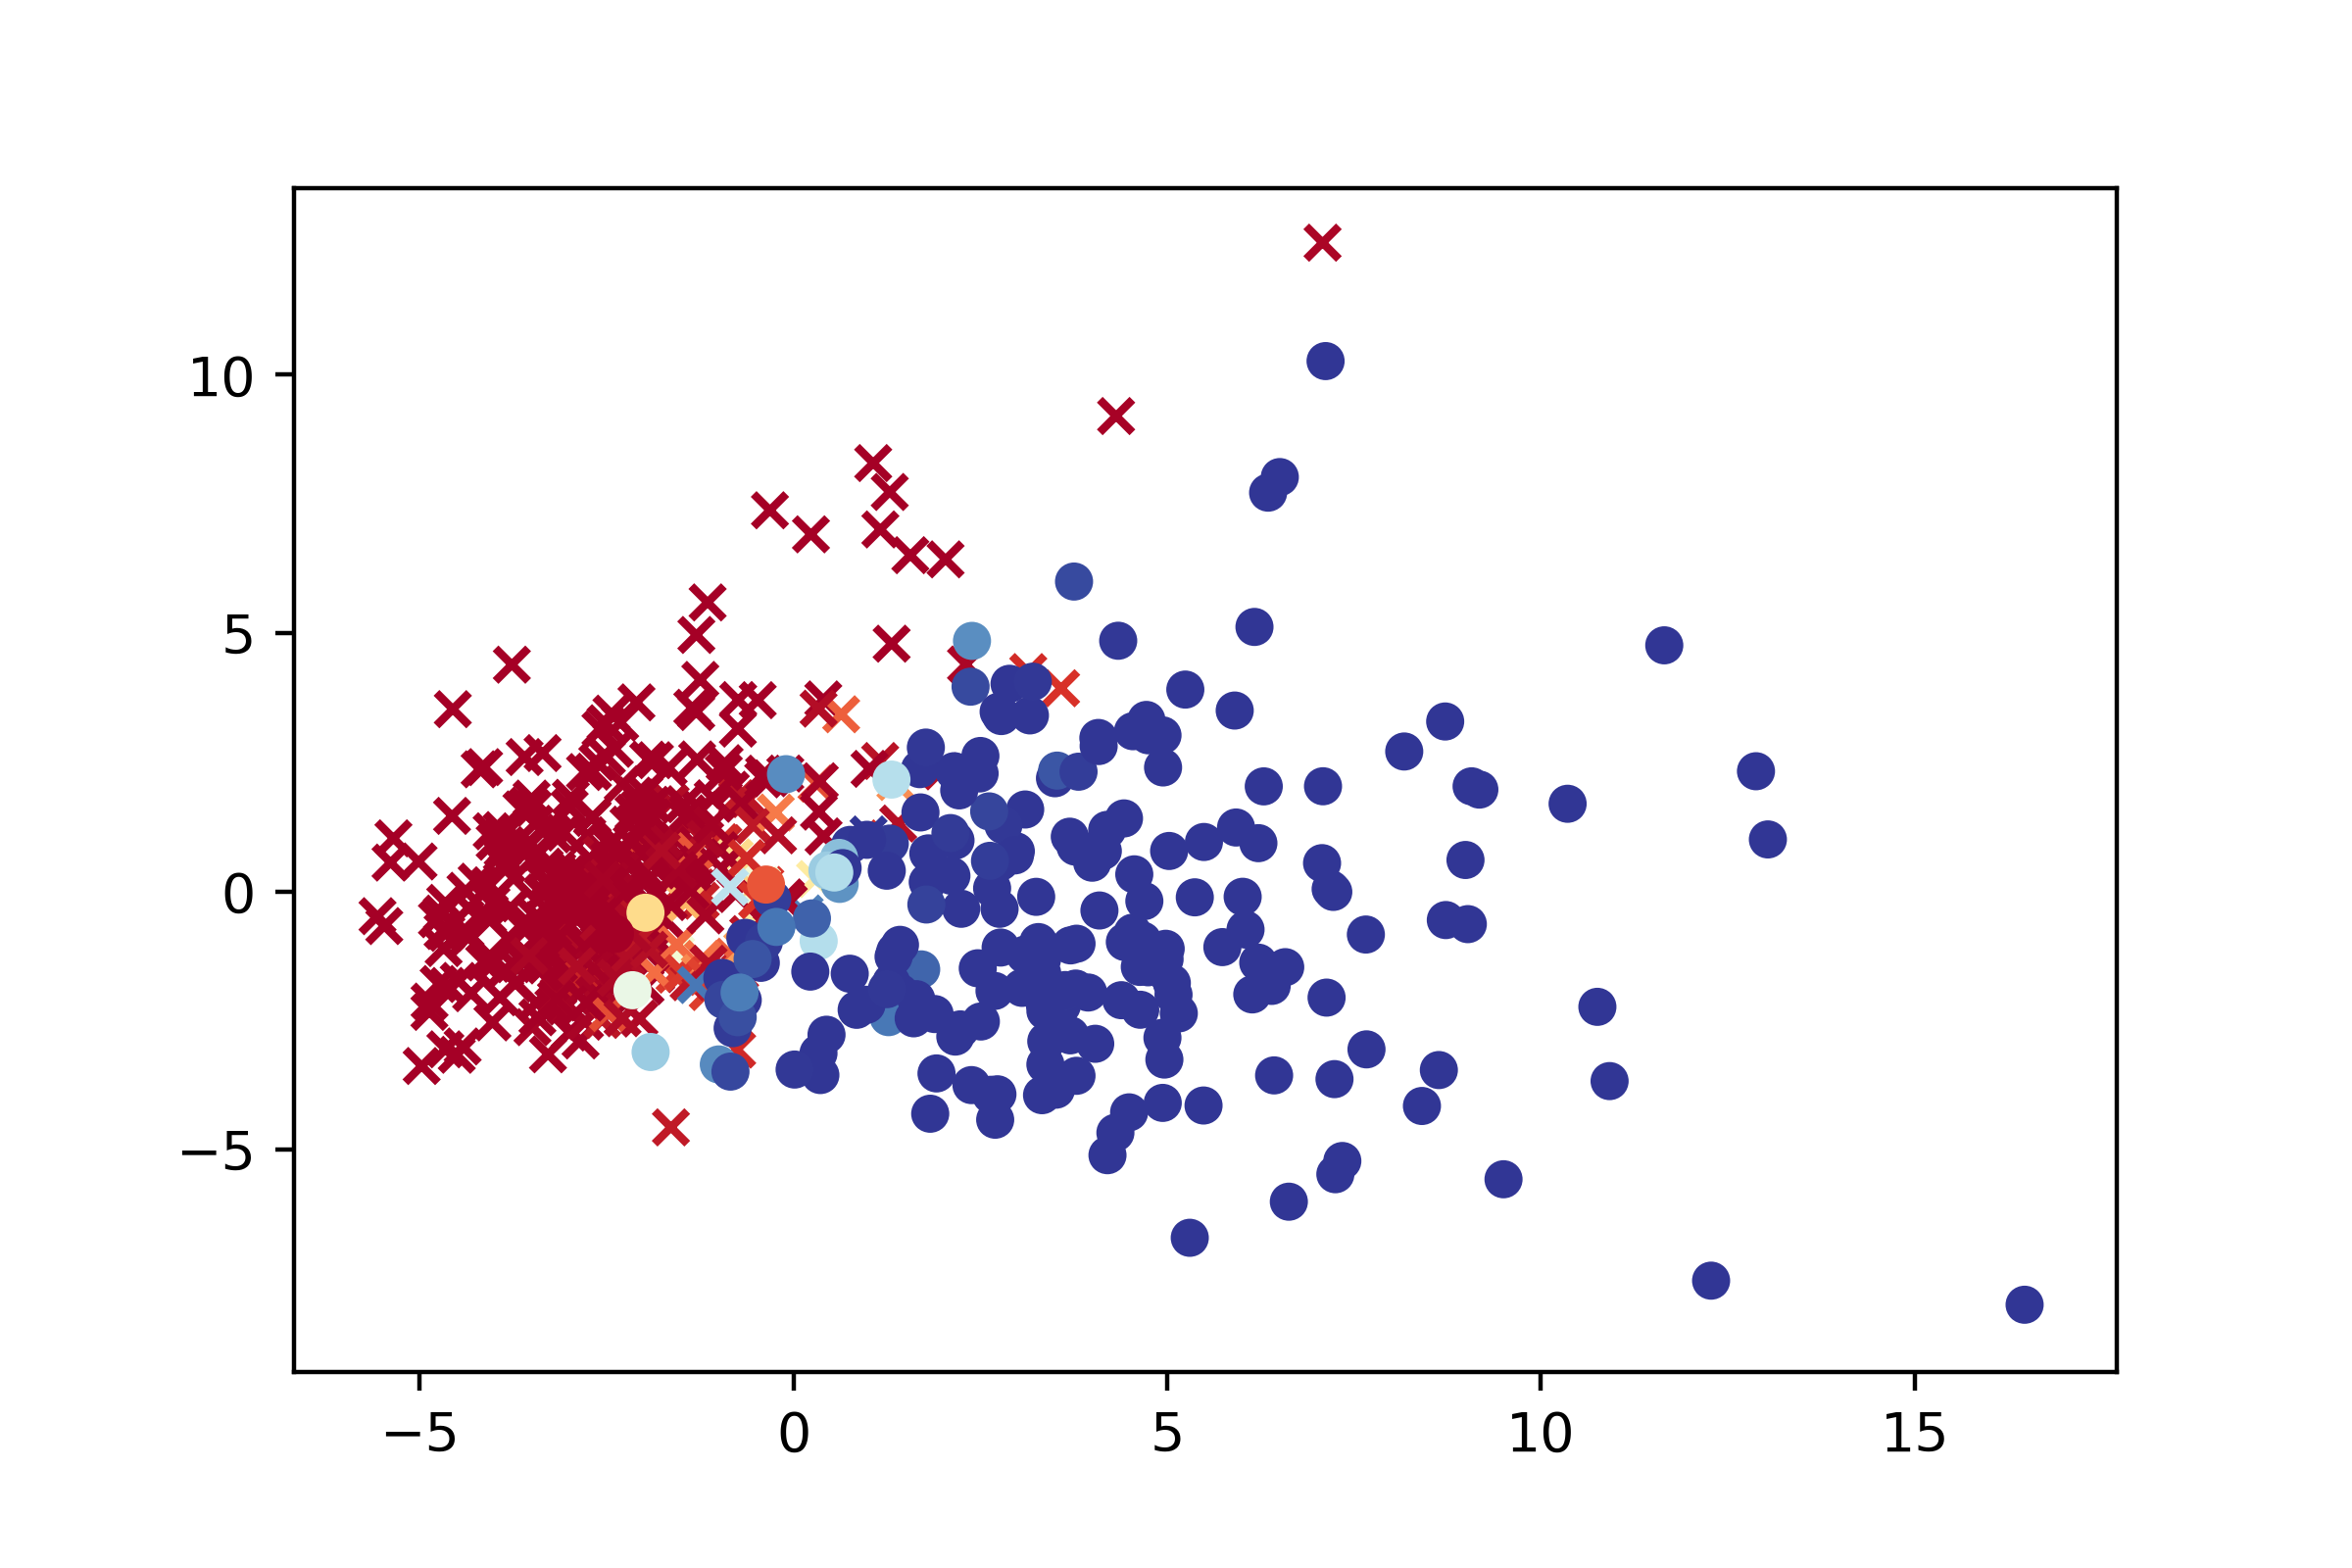
\includegraphics[width=0.80\textwidth]{fig/plt/bc.png} \tabularnewline
    
%     Sloan Sky Survey & 
%     %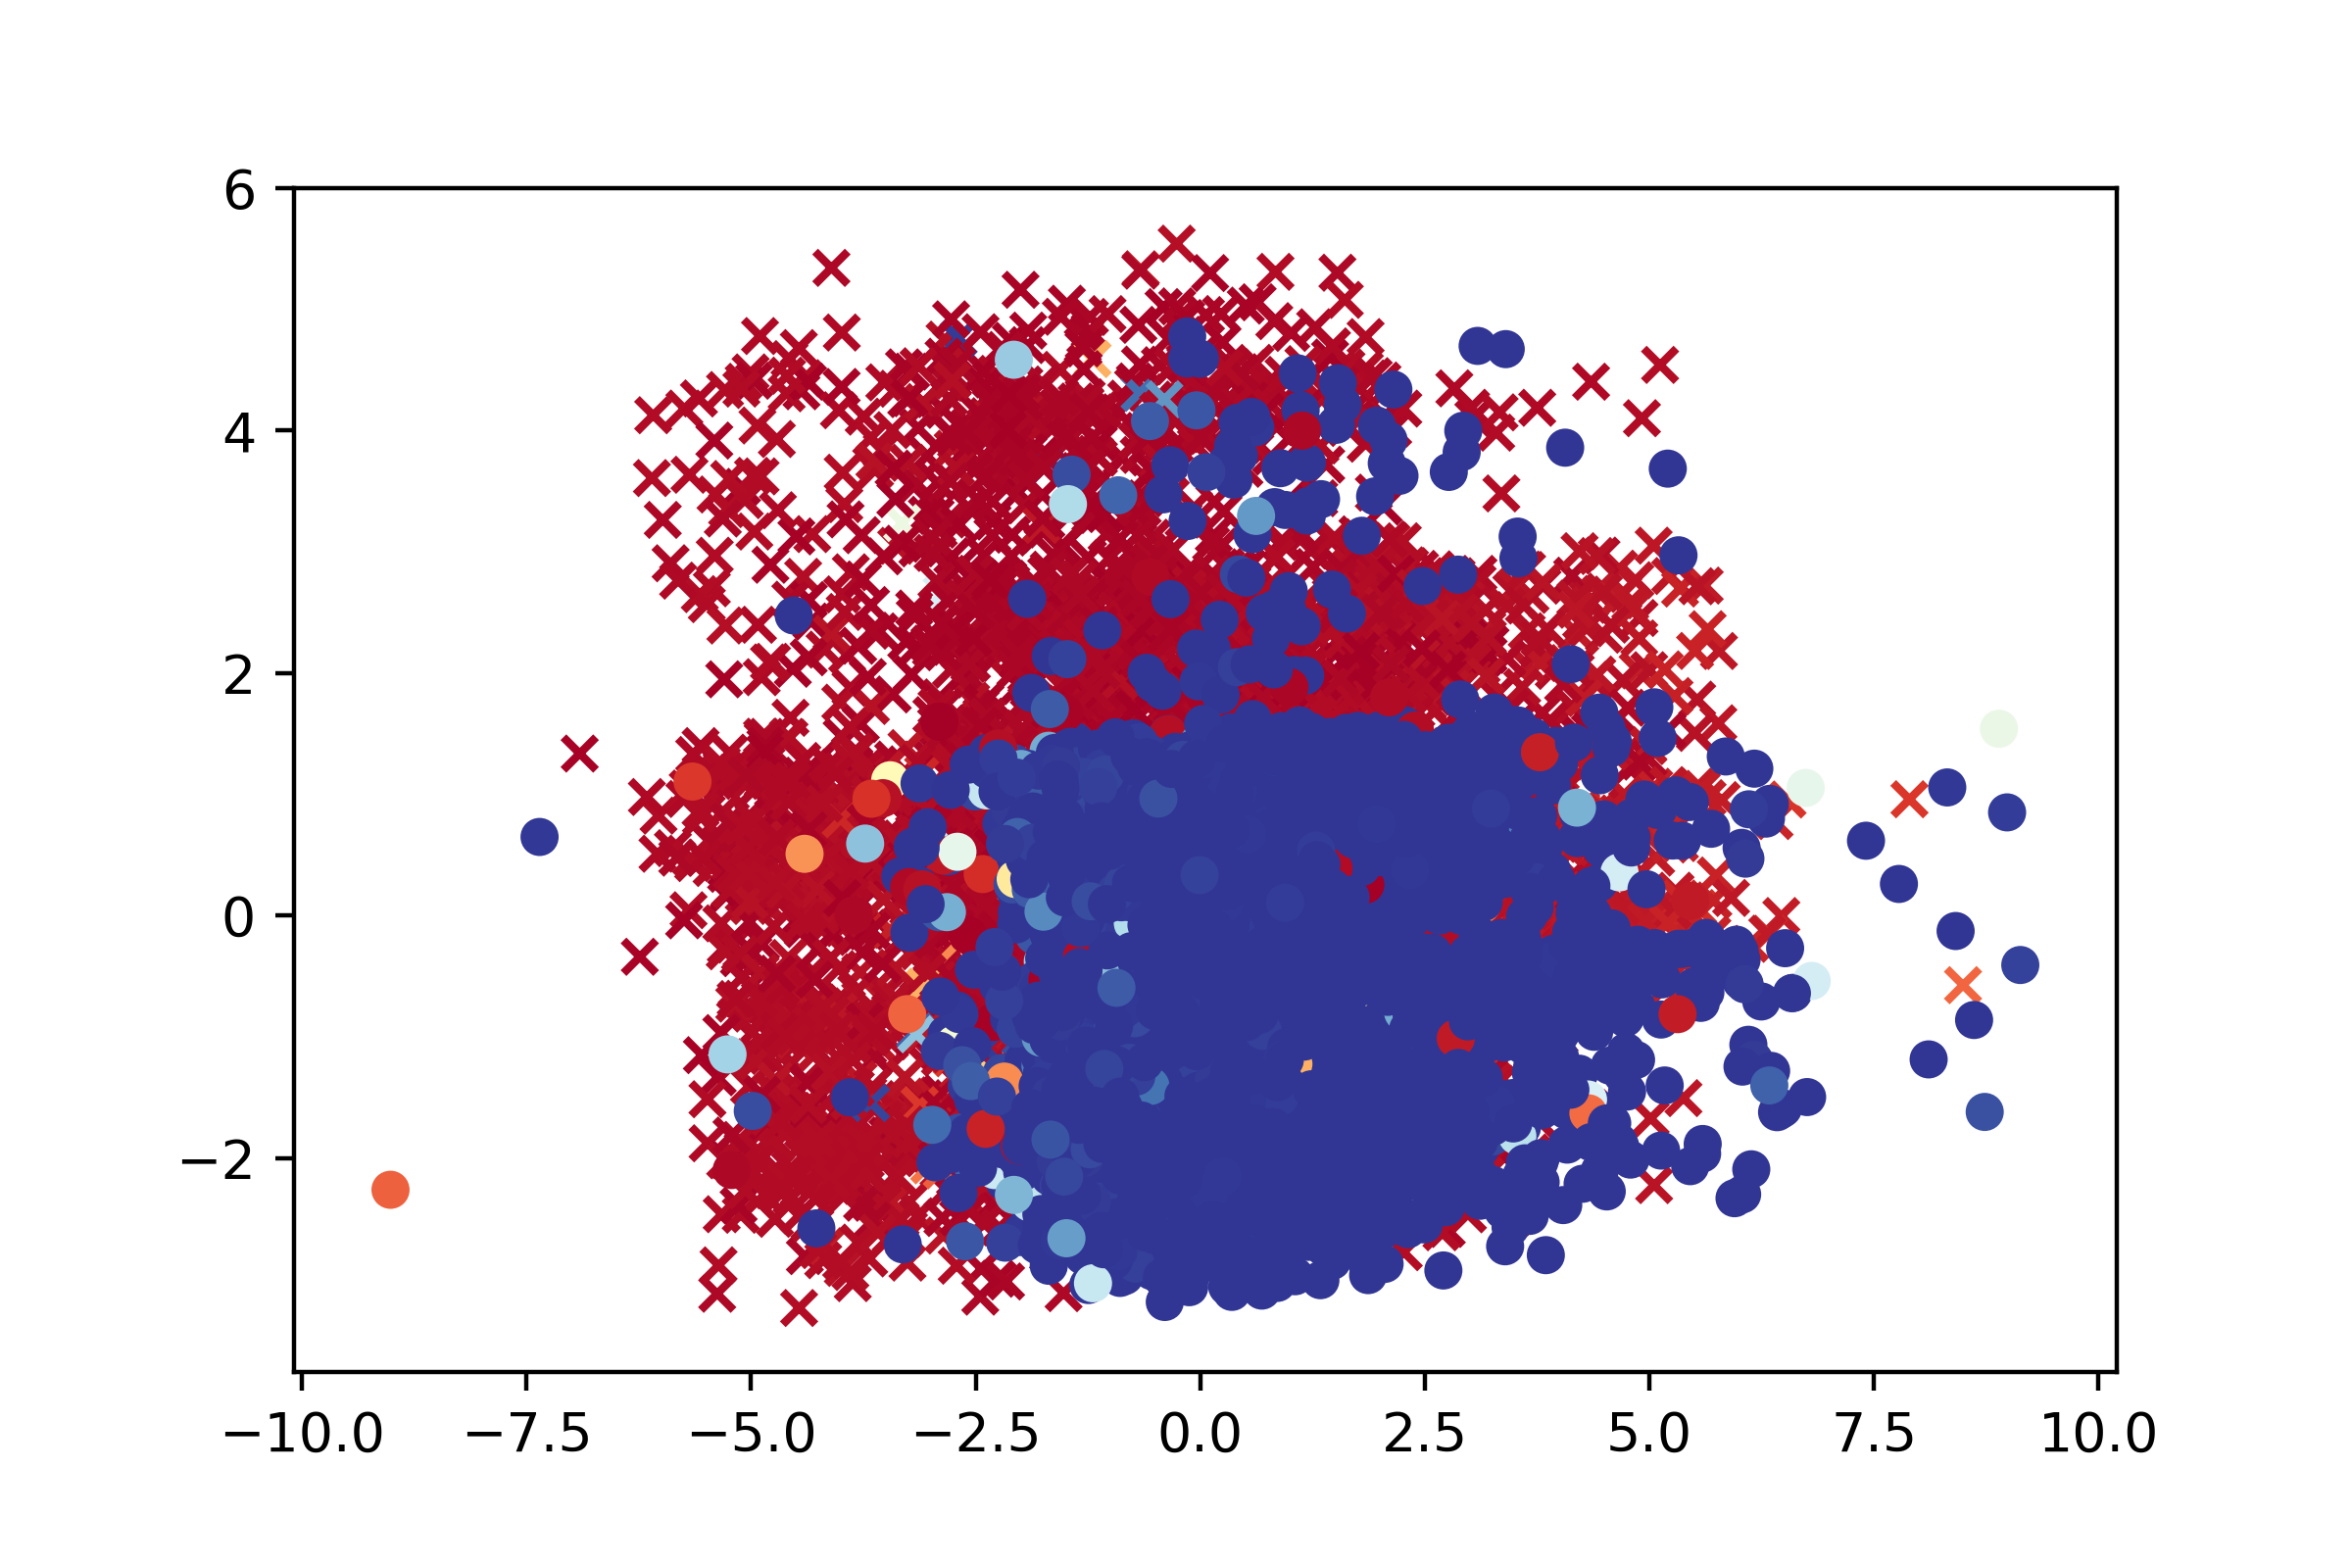
\includegraphics[width=0.22\textwidth]{fig/plt/st.png} &
%     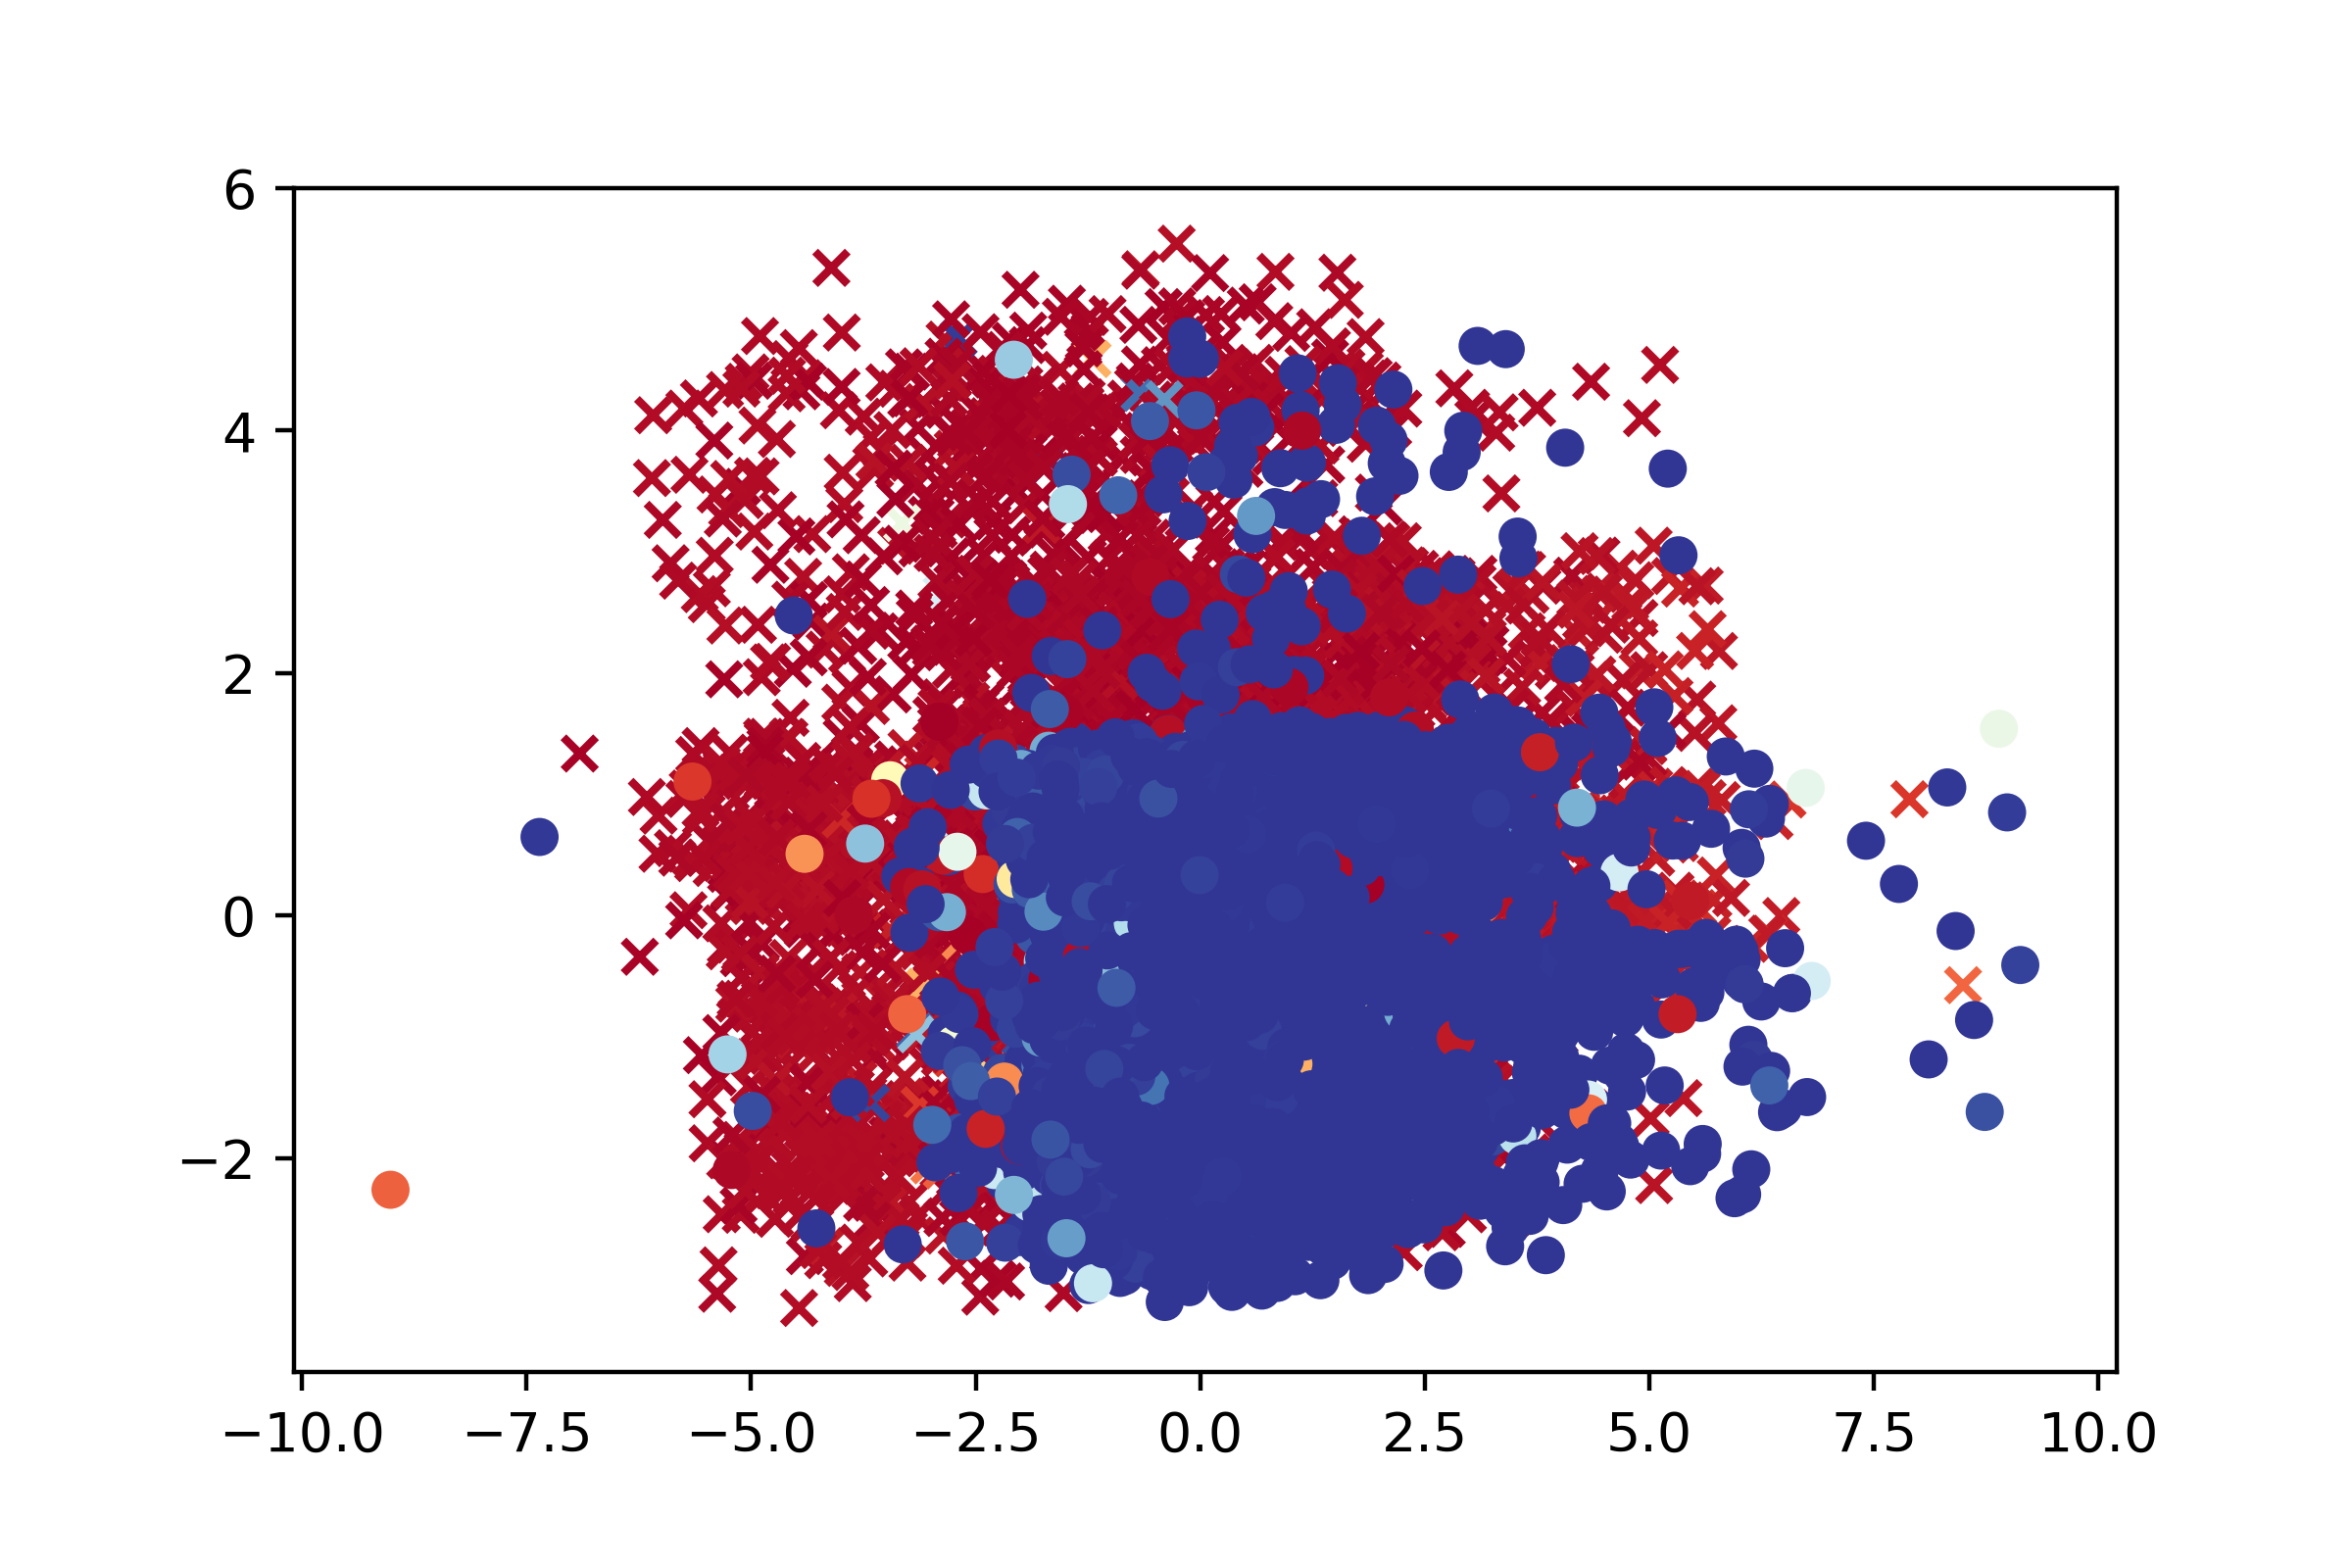
\includegraphics[width=0.80\textwidth]{fig/plt/st.png} \tabularnewline
    
%     Iris & 
%     %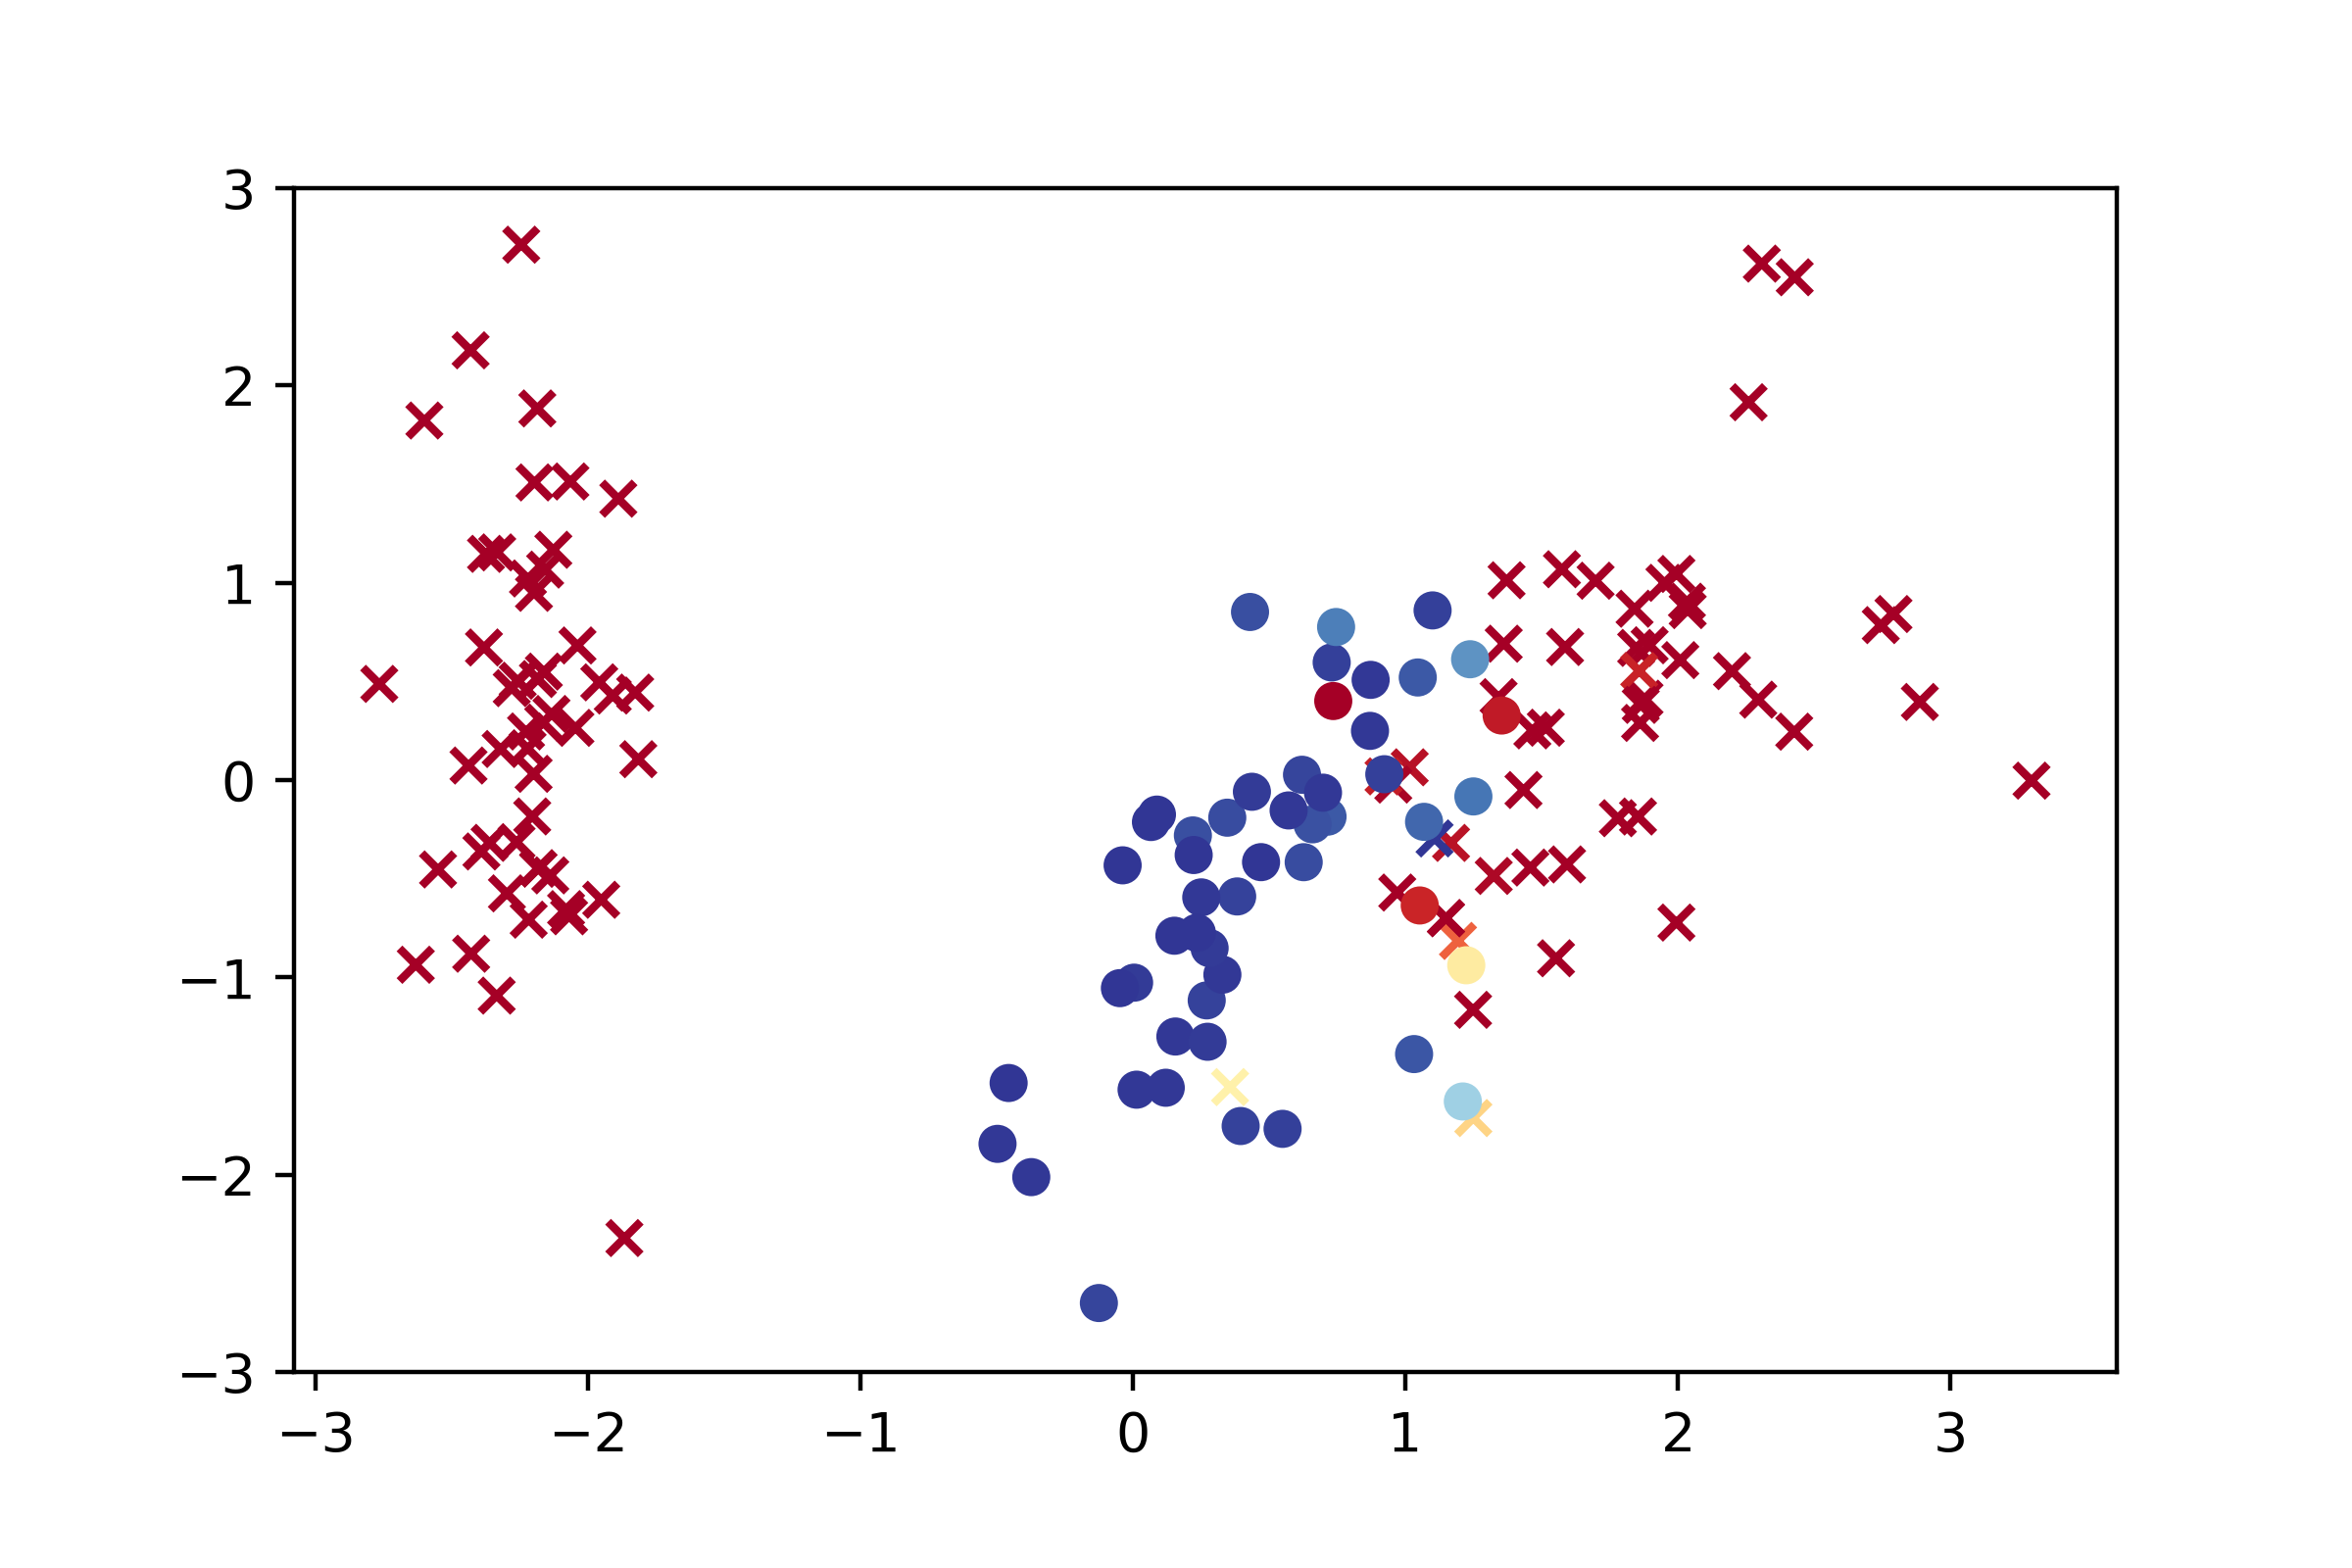
\includegraphics[width=0.22\textwidth]{fig/plt/ir.png} &
%     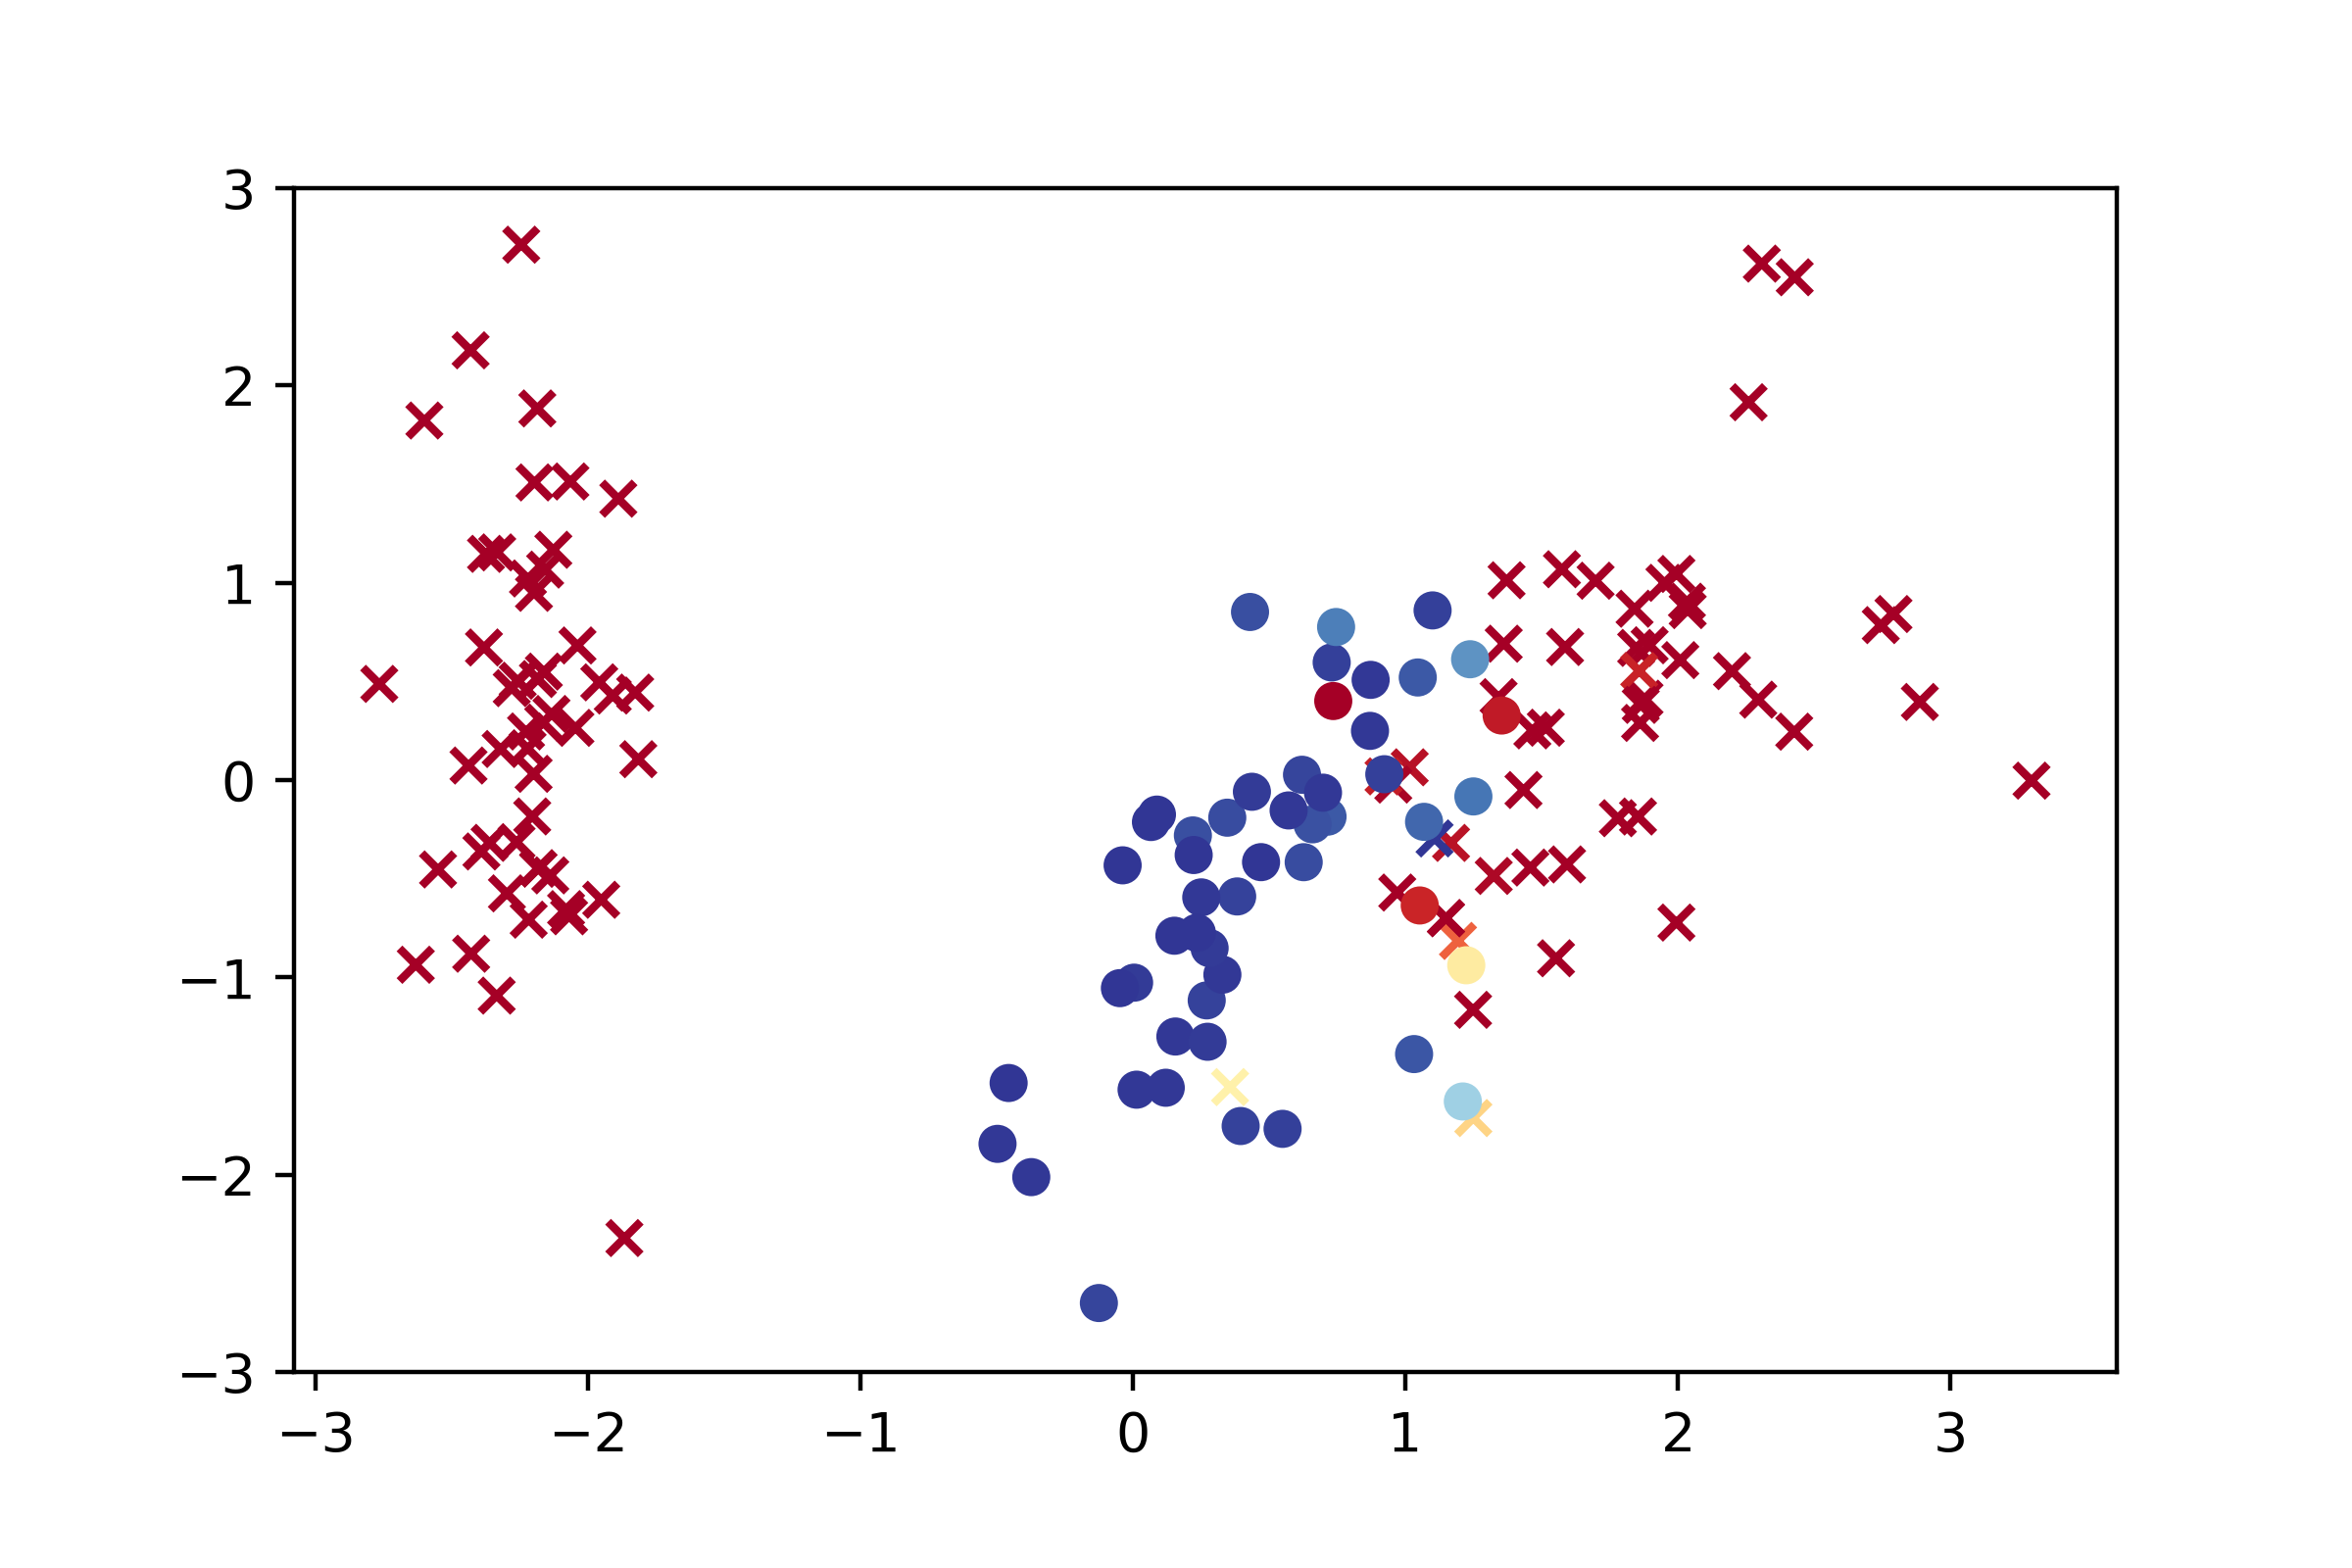
\includegraphics[width=0.80\textwidth]{fig/plt/ir.png} \tabularnewline
    
%     Titanic & 
%     %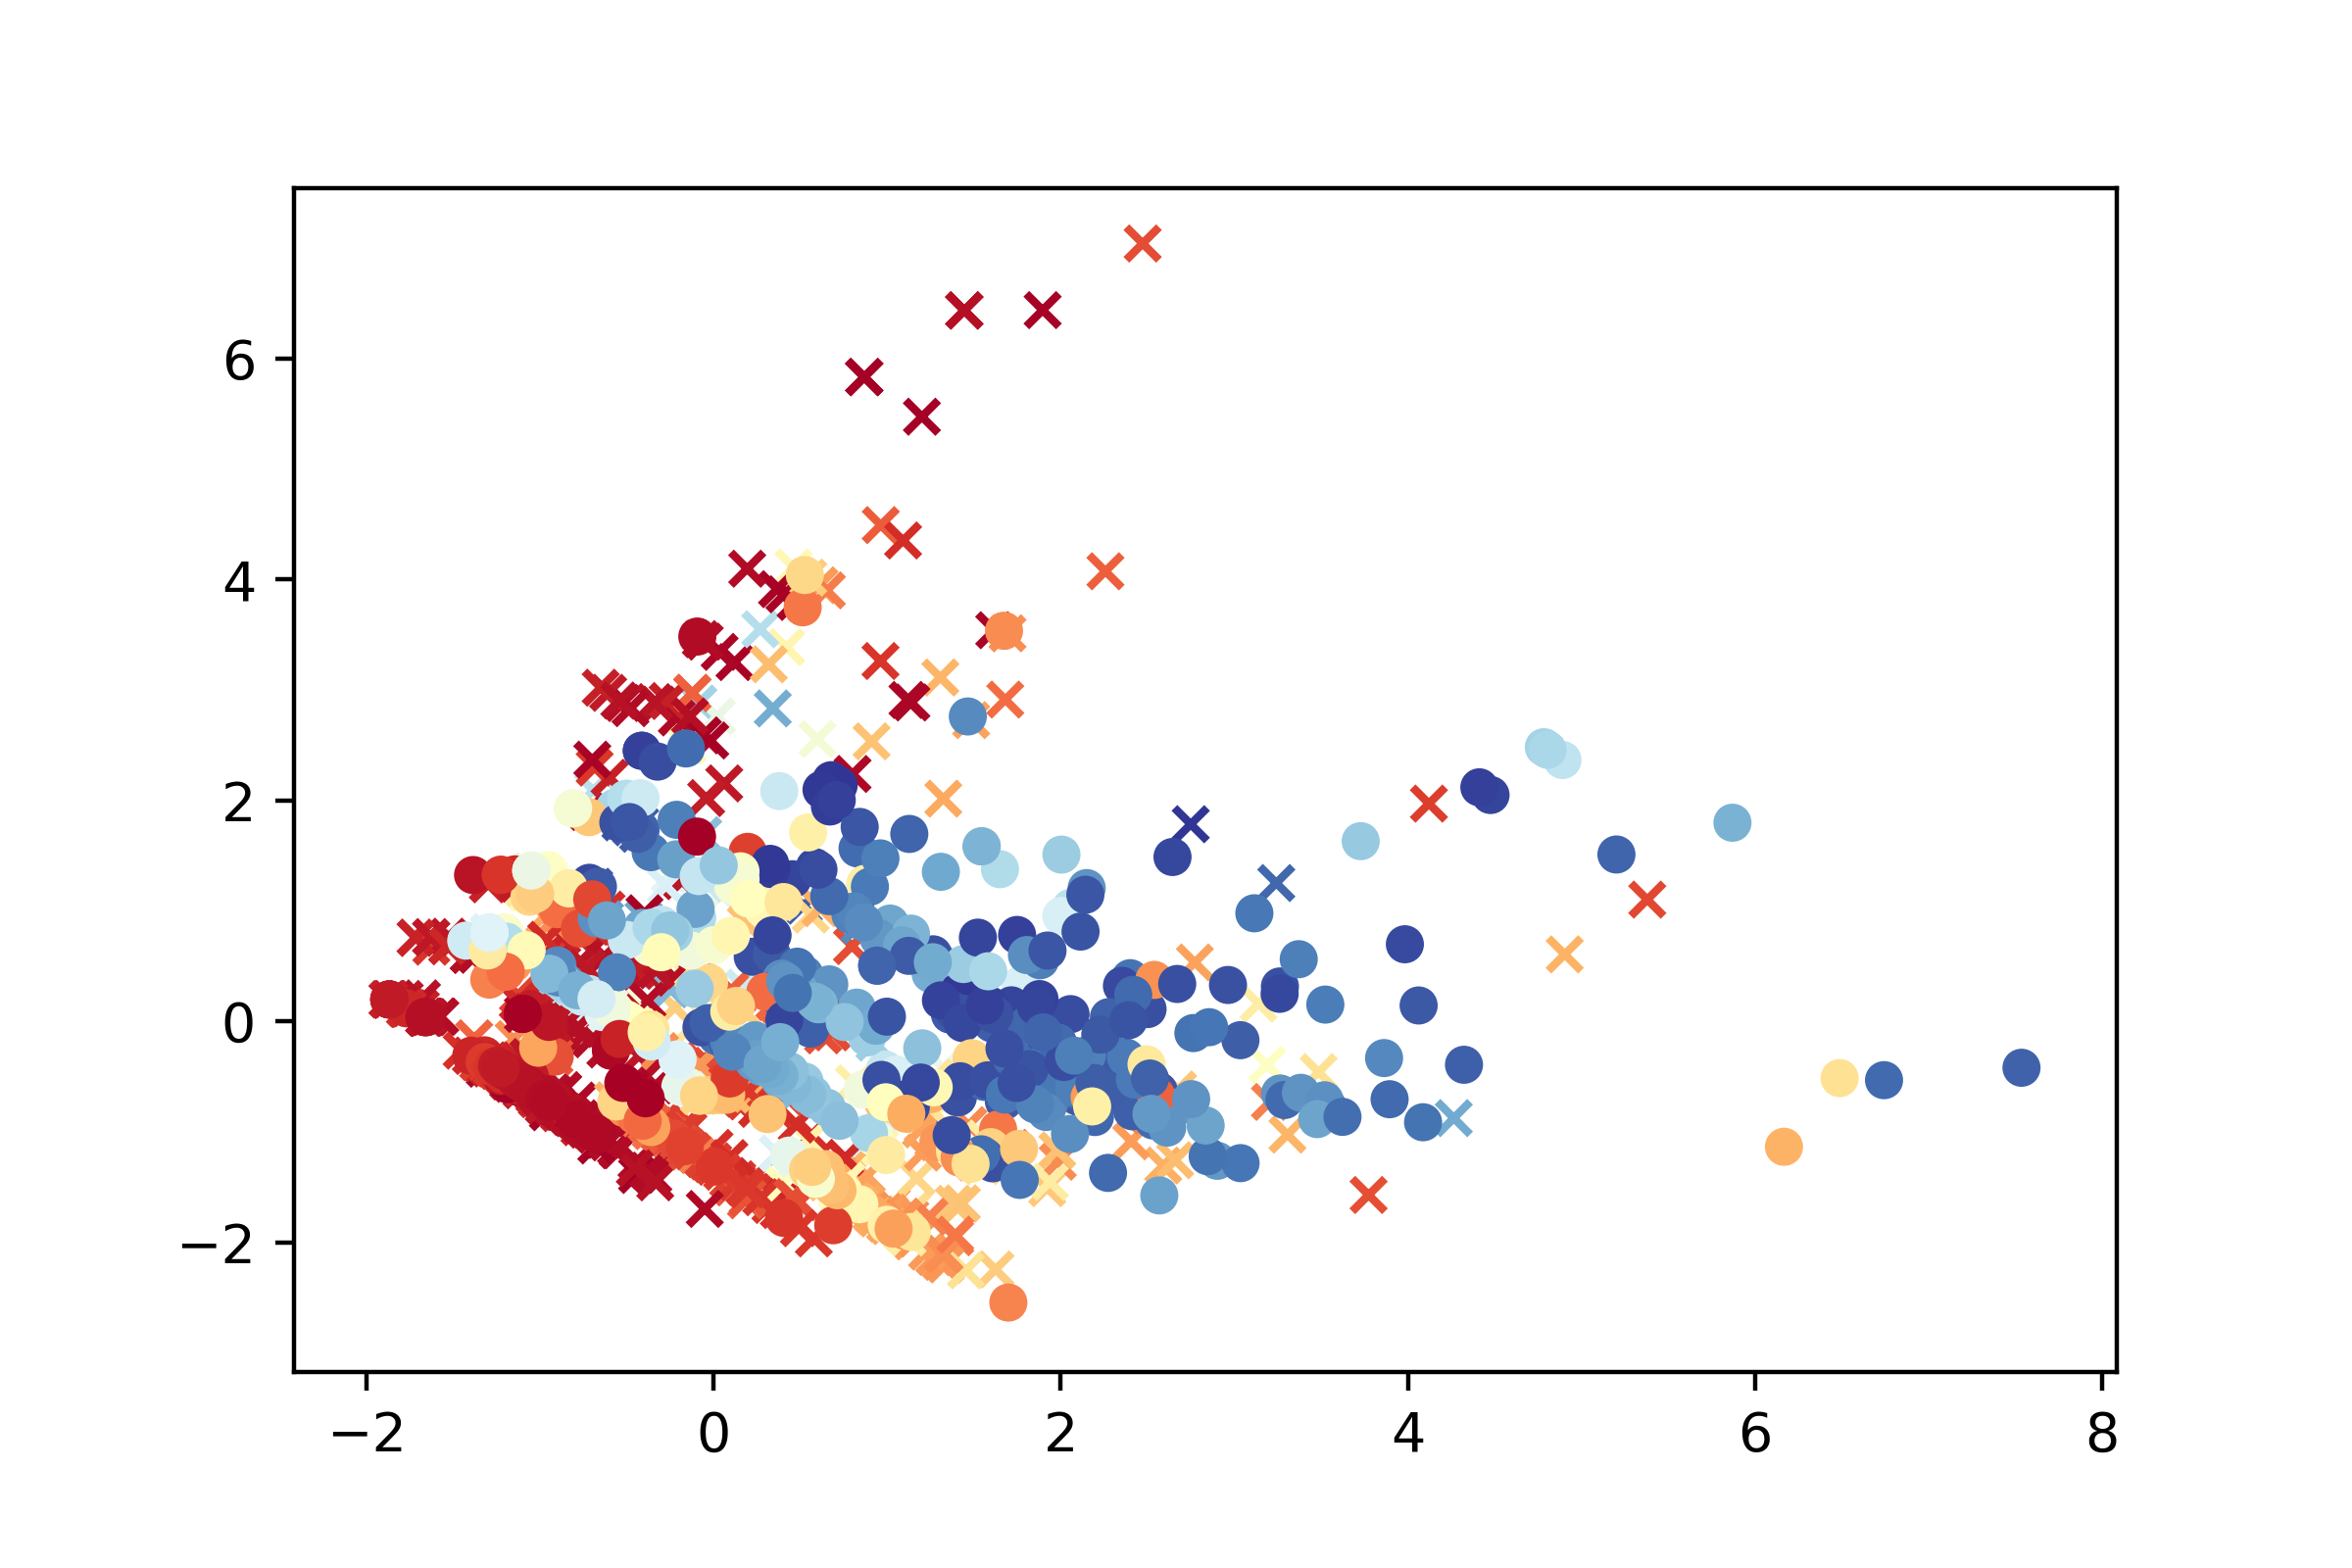
\includegraphics[width=0.22\textwidth]{fig/plt/ti.png} &
%     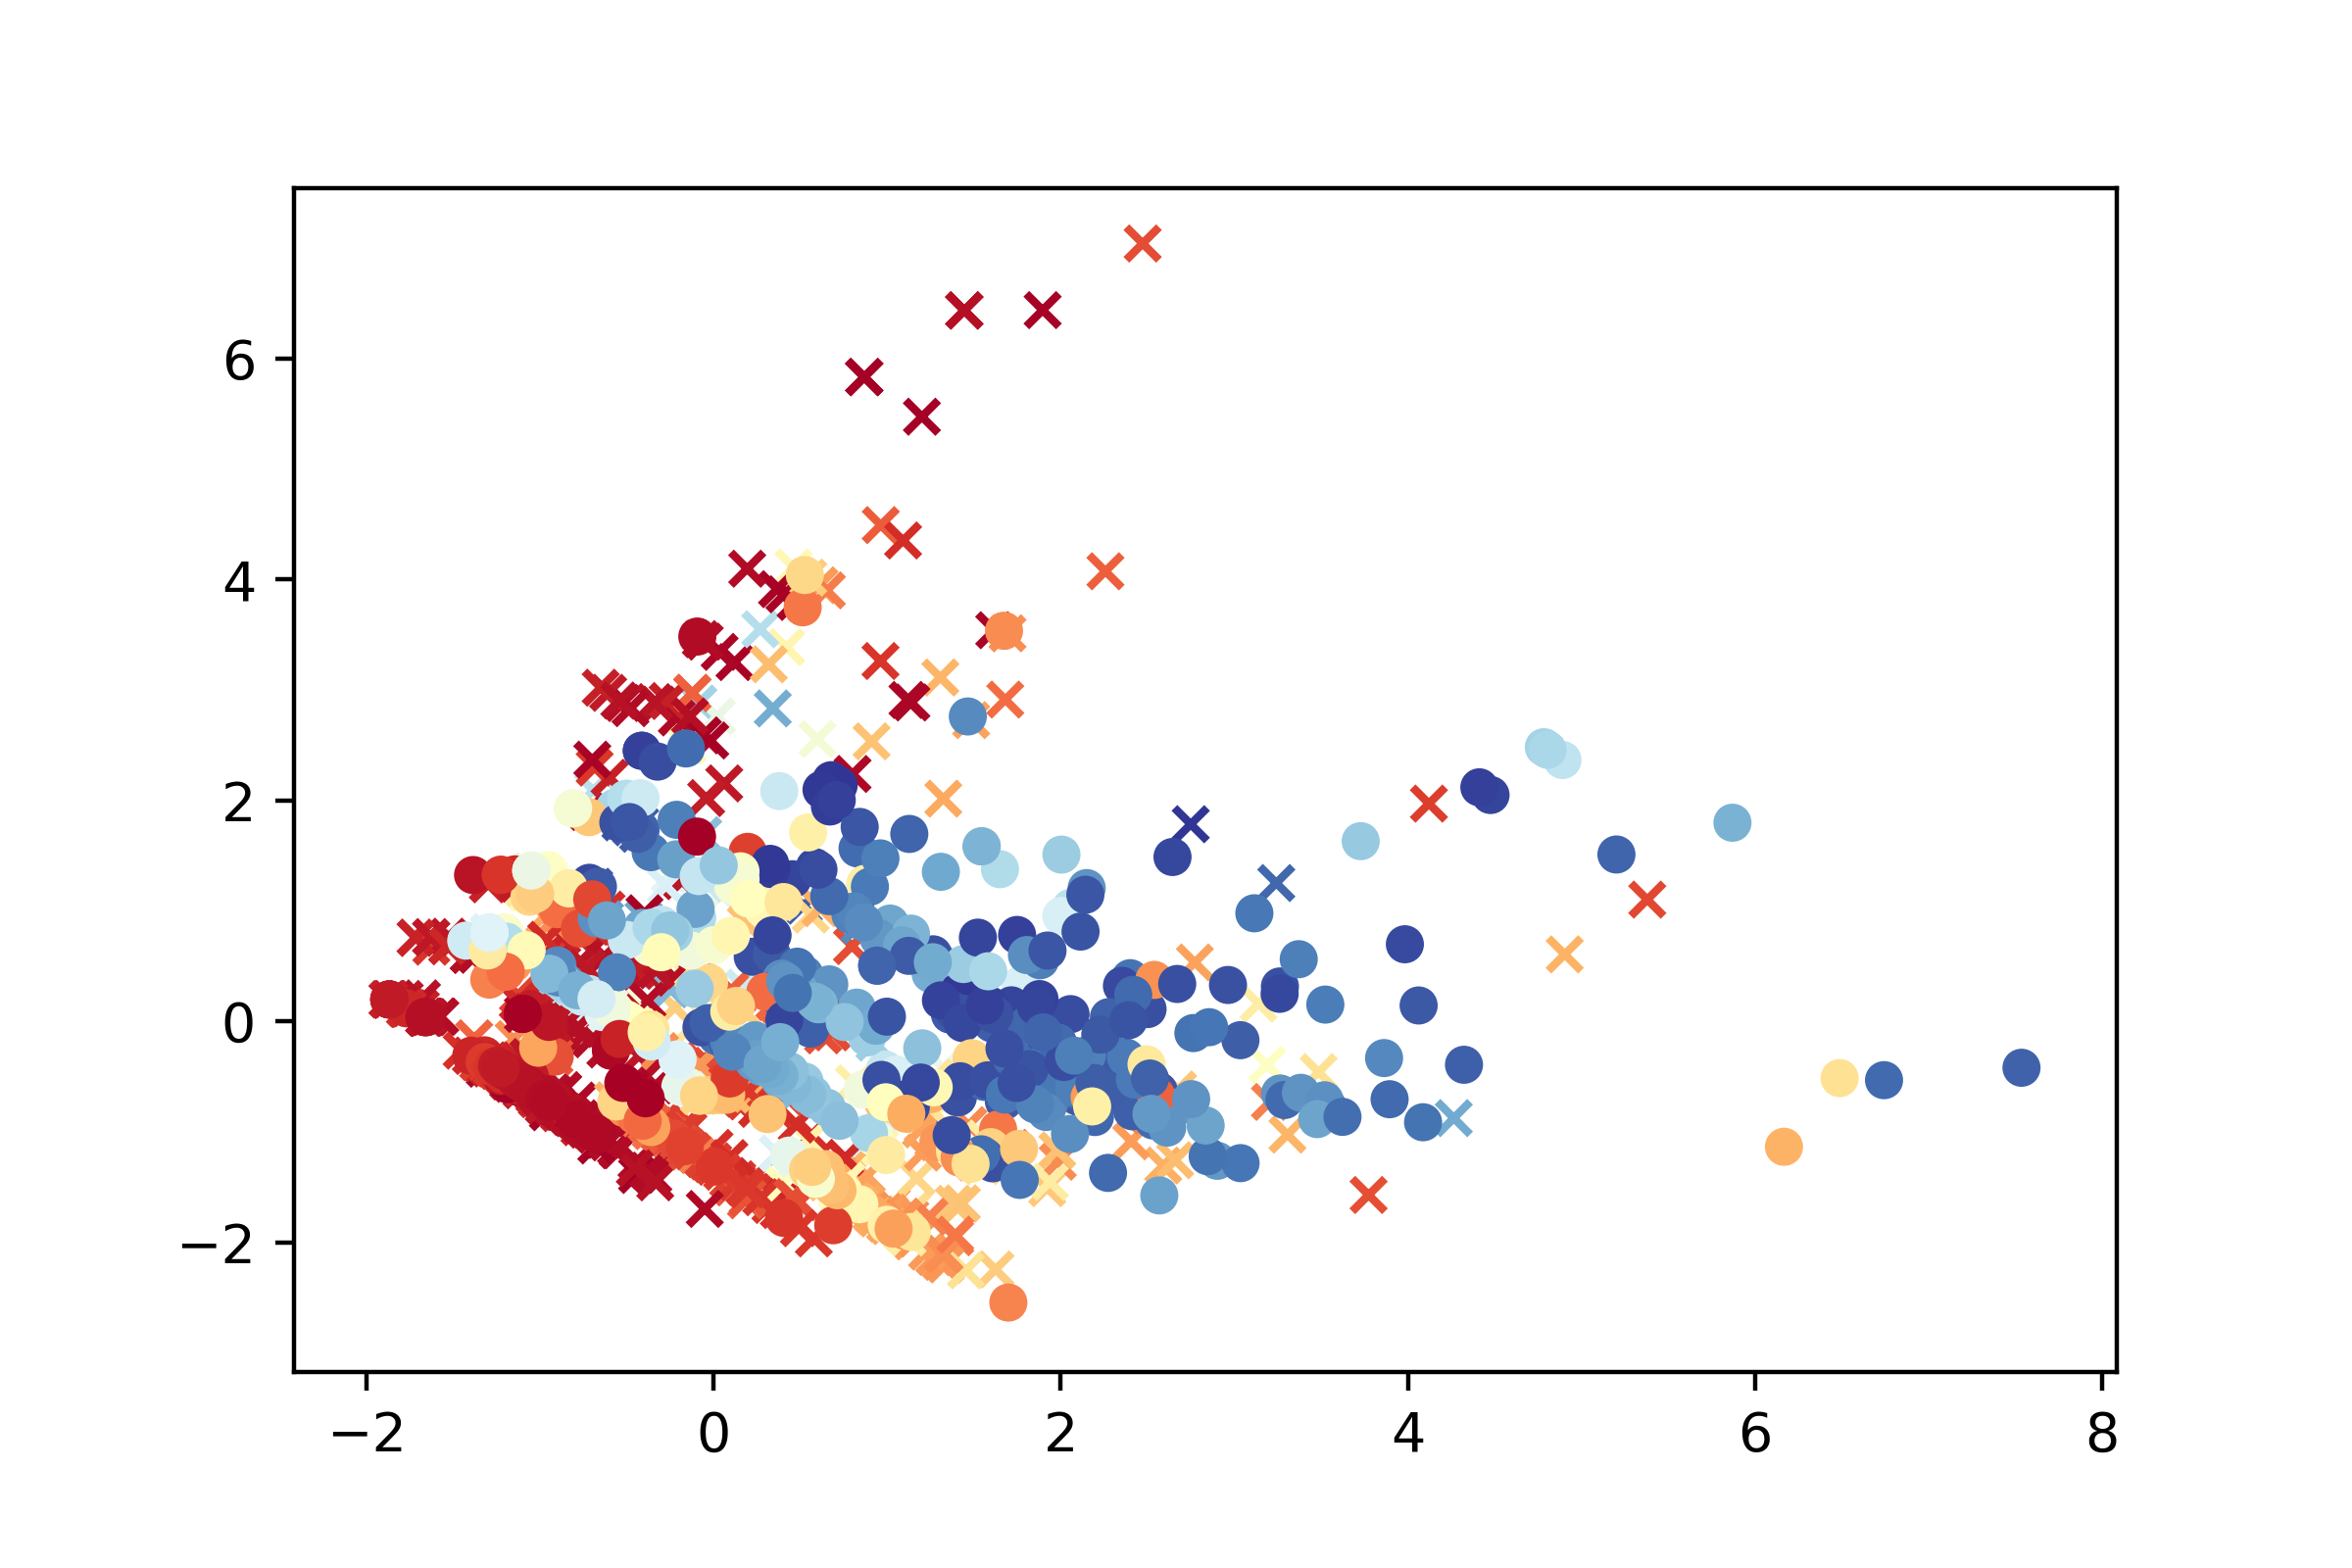
\includegraphics[width=0.80\textwidth]{fig/plt/ti.png} \tabularnewline
    
%     Wine & 
%     %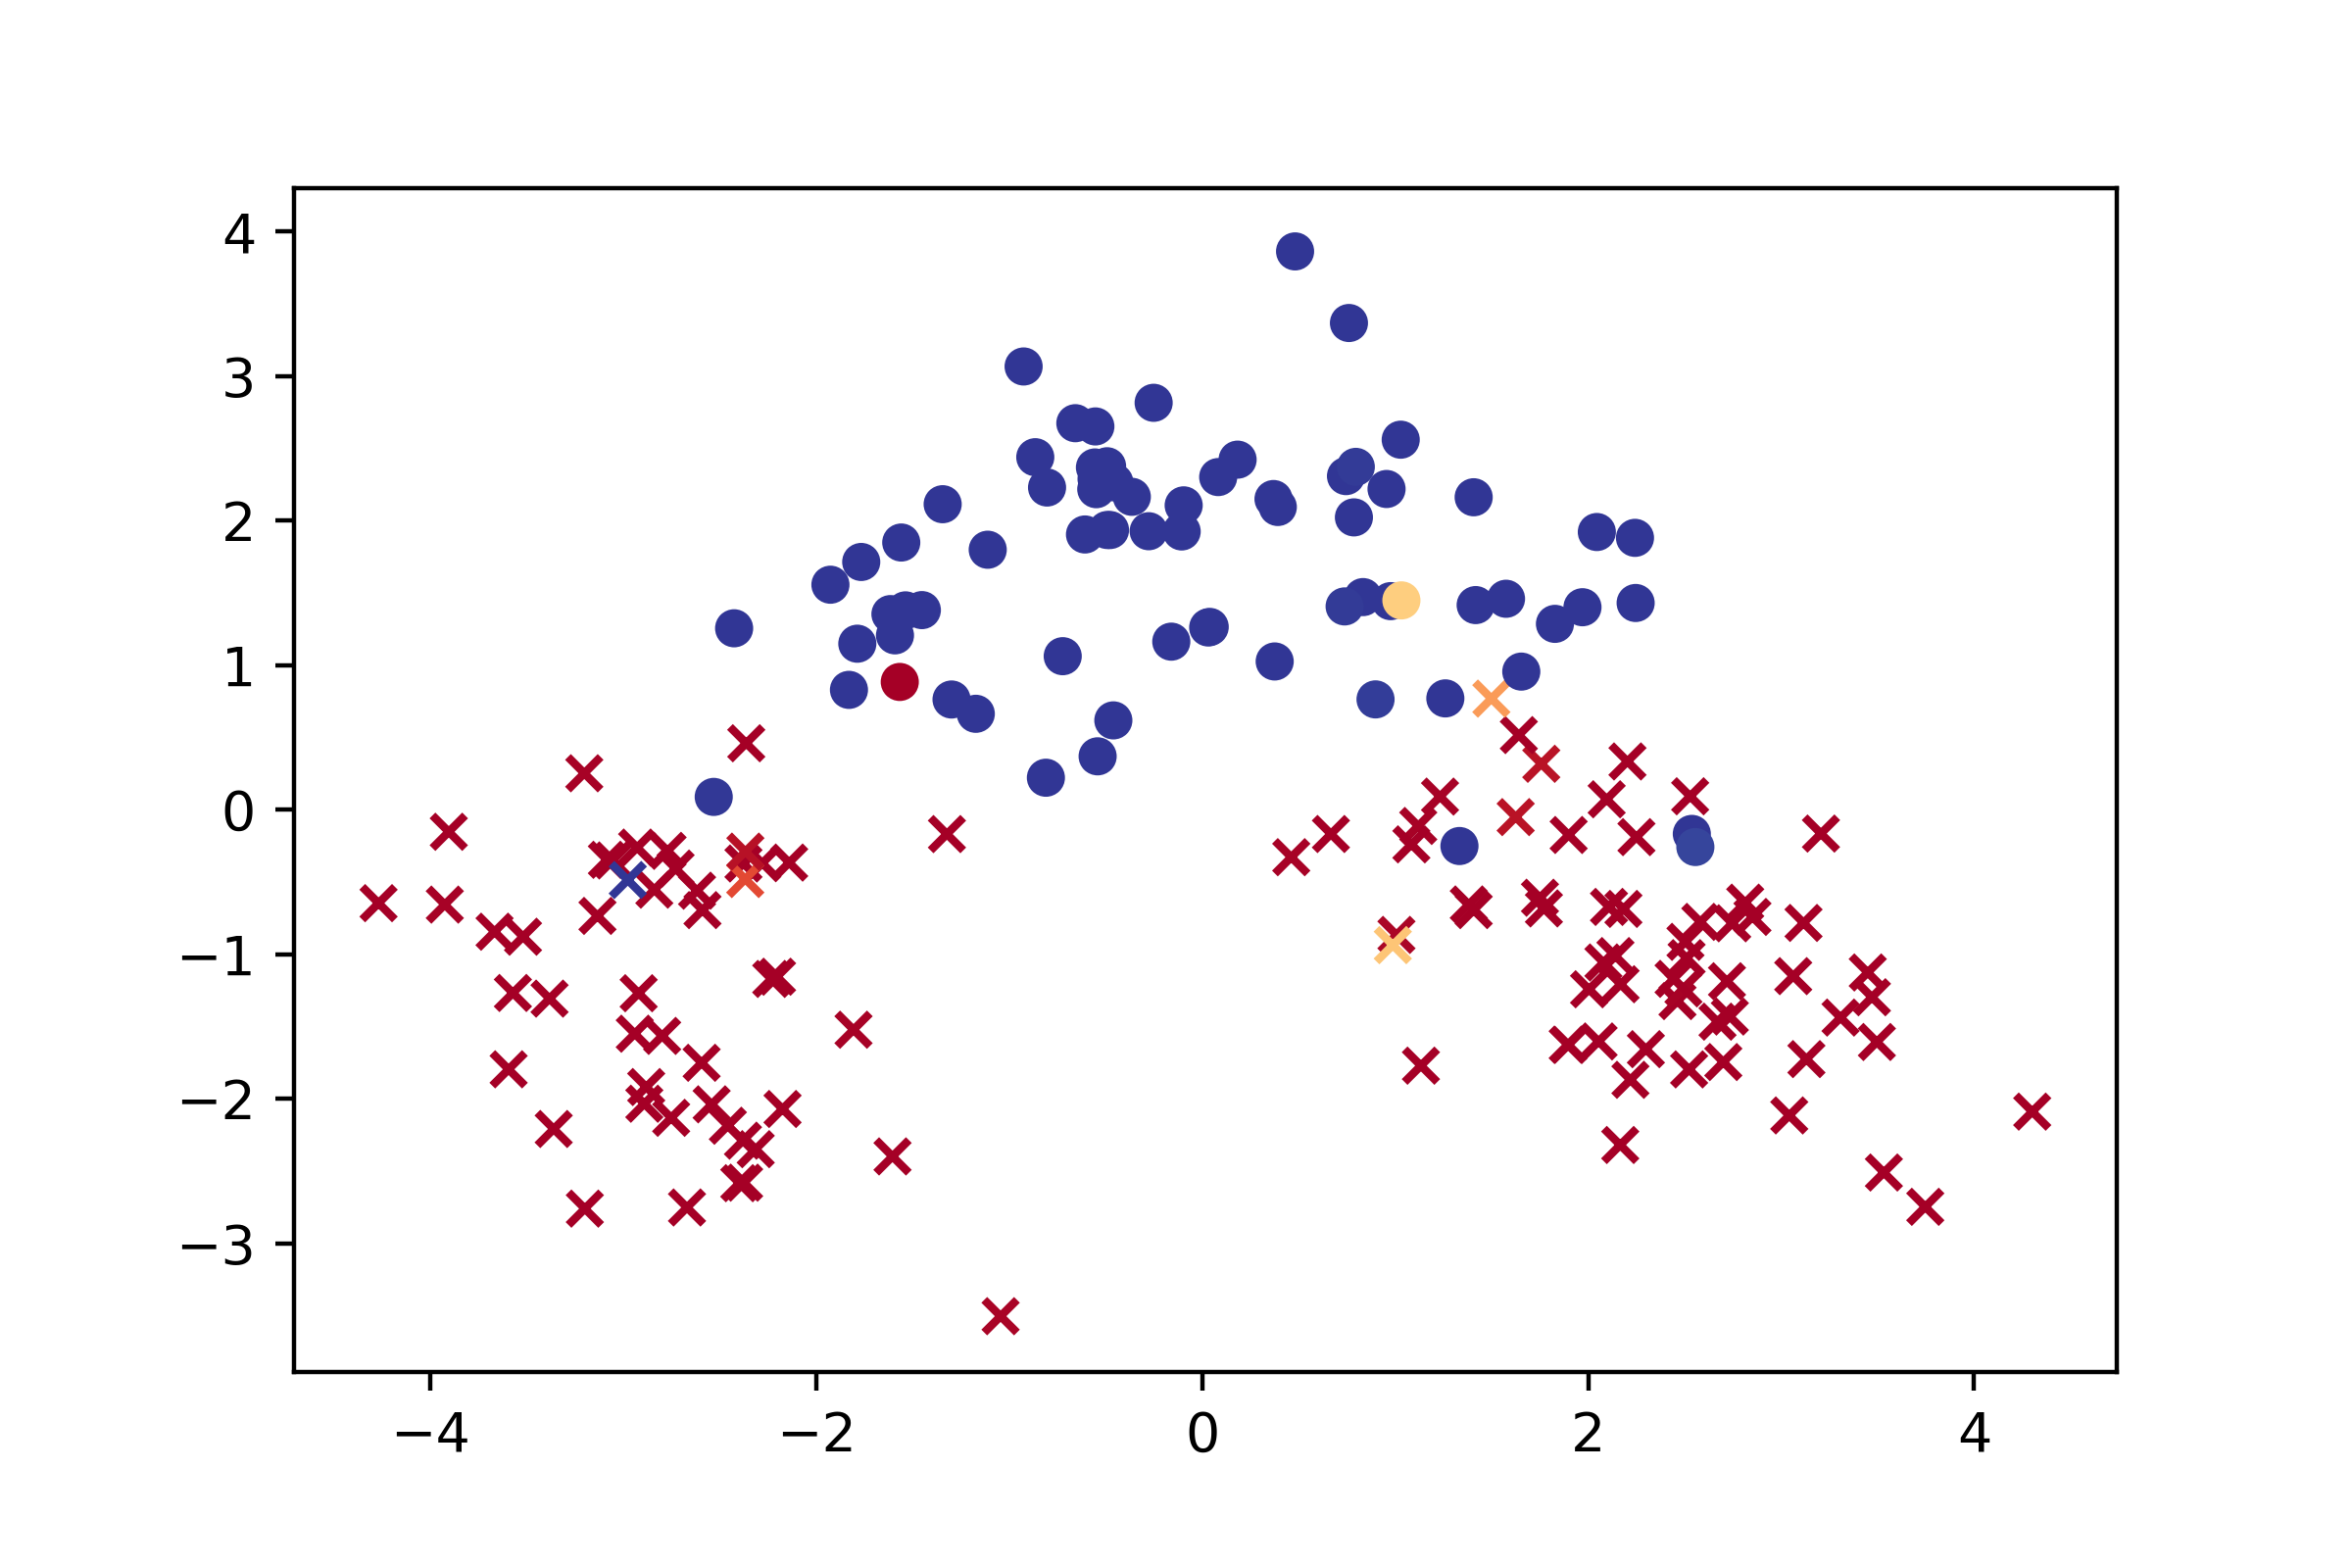
\includegraphics[width=0.22\textwidth]{fig/plt/wi.png} &
%     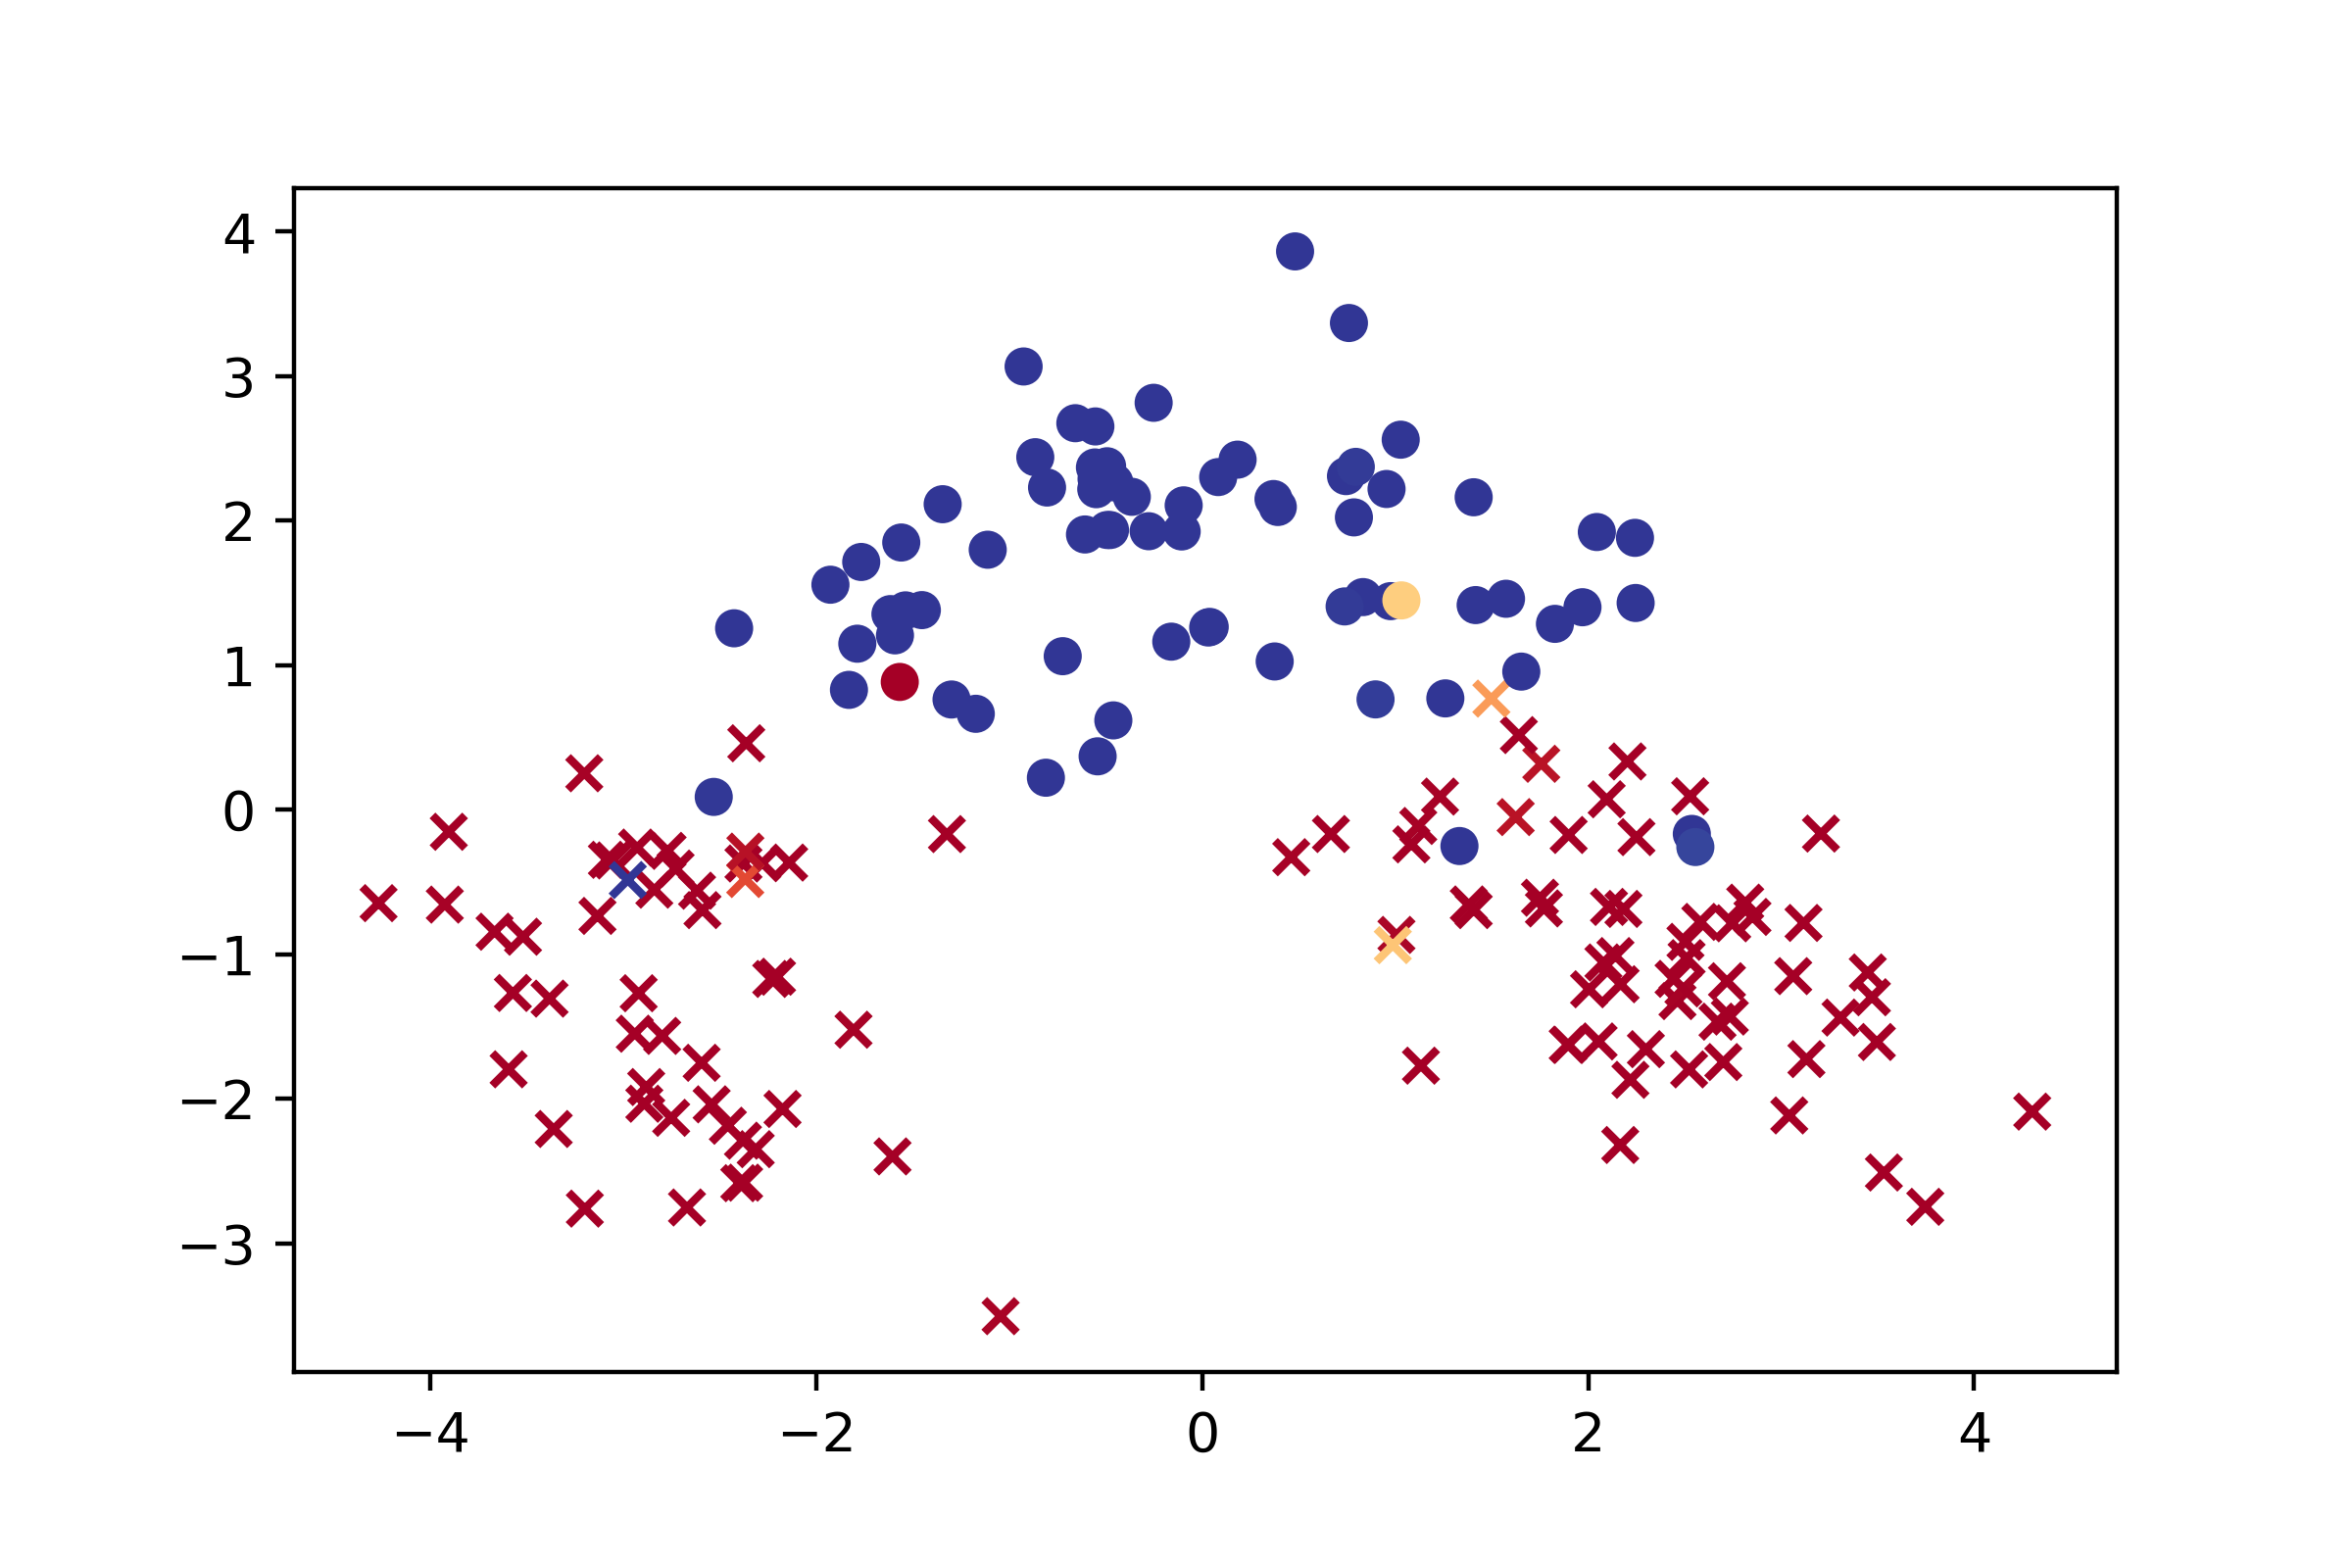
\includegraphics[width=0.80\textwidth]{fig/plt/wi.png} \tabularnewline
    
%     % Circle & 
%     % 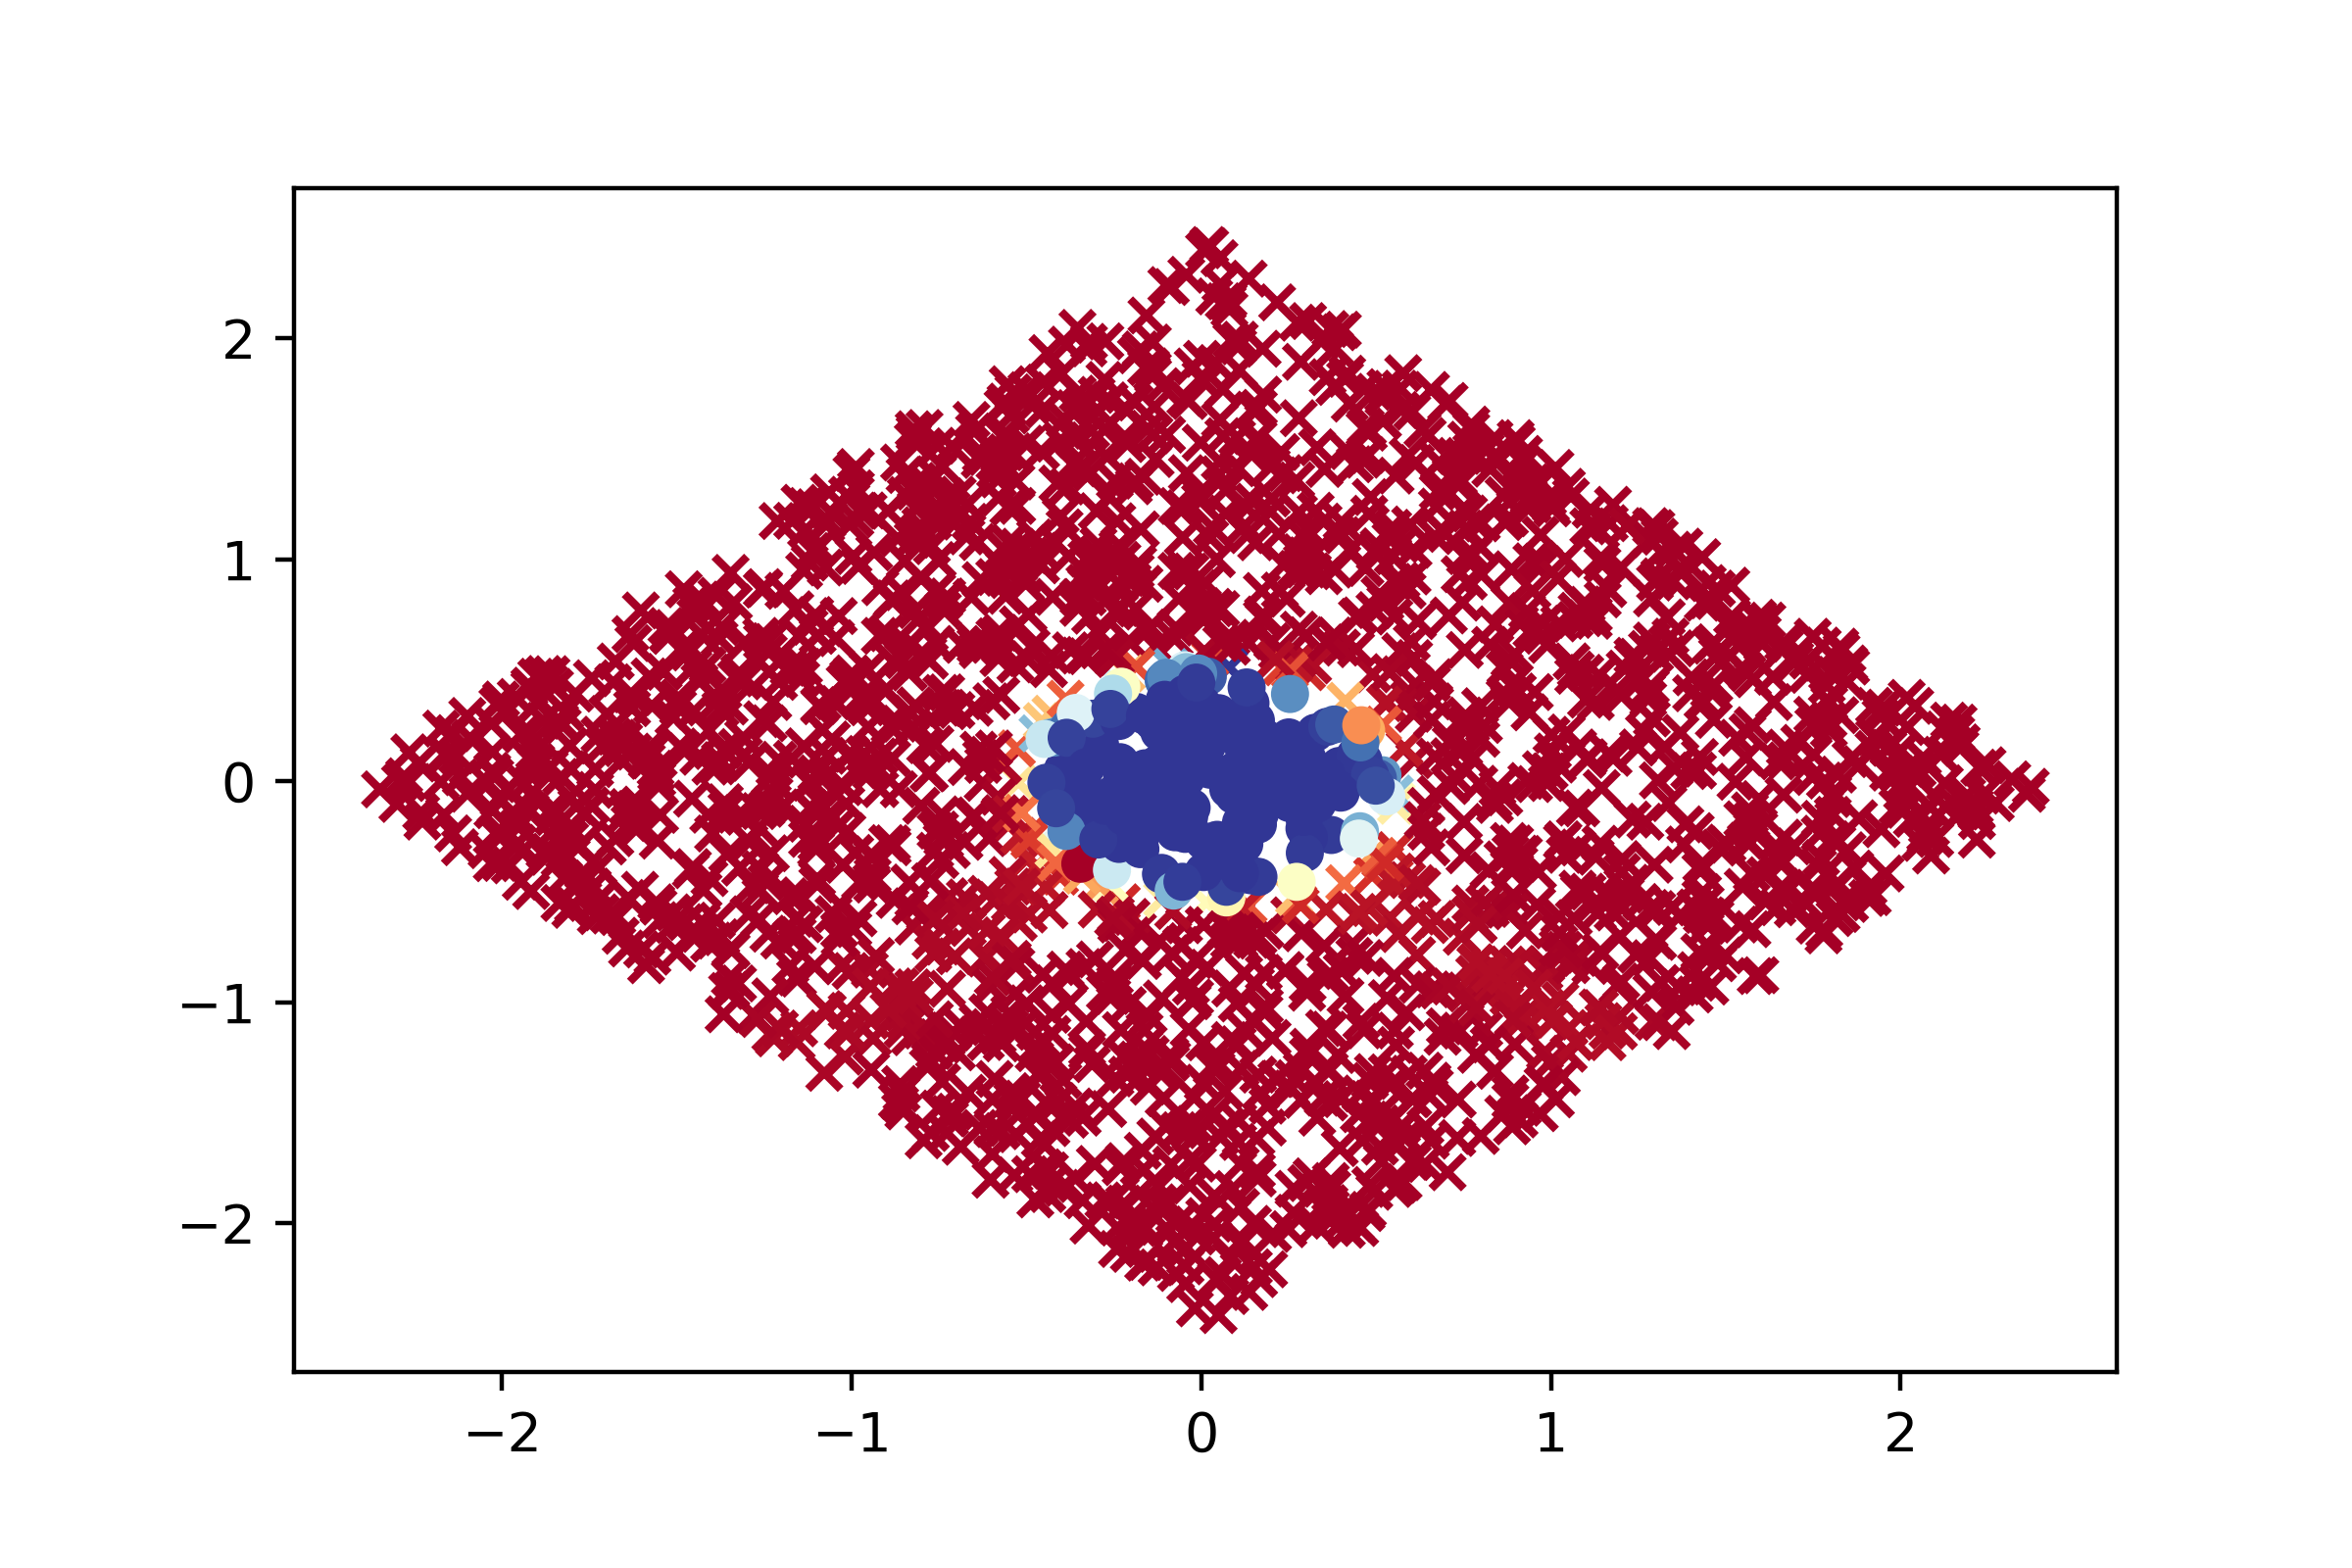
\includegraphics[width=0.22\textwidth]{fig/plt/ci.png} &
%     % 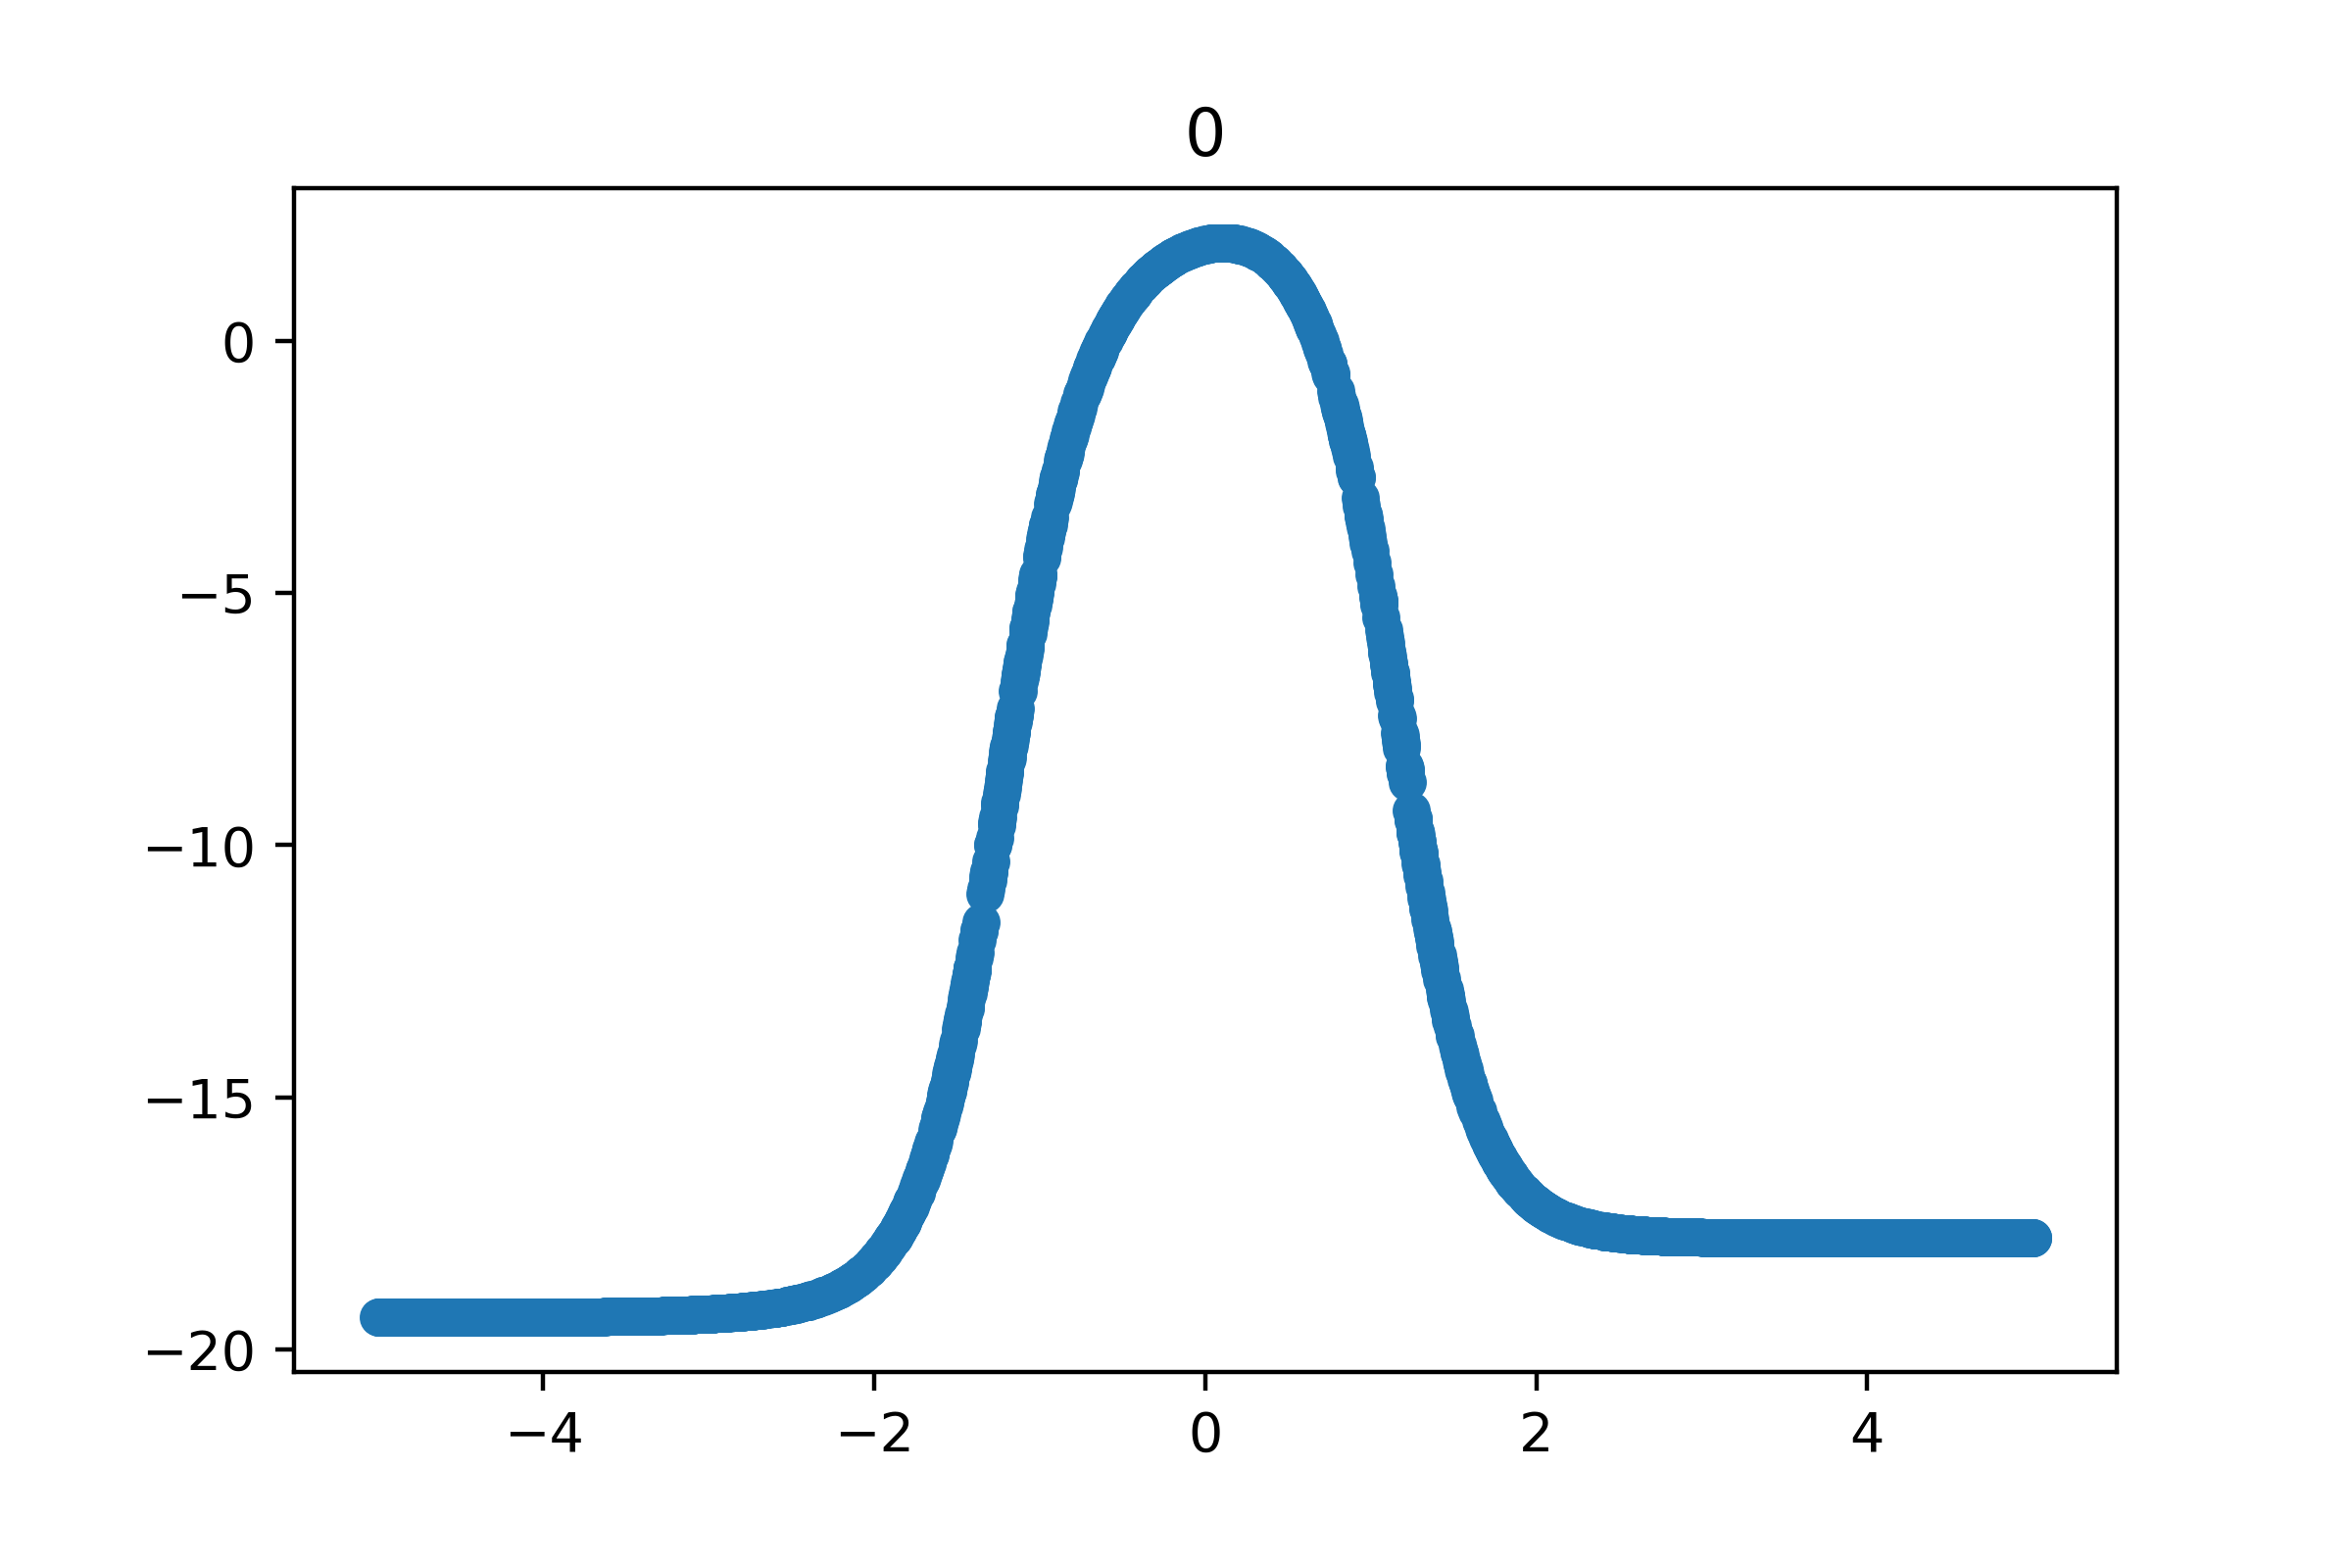
\includegraphics[width=0.22\textwidth]{fig/mnl/ci1.png} &
%     % 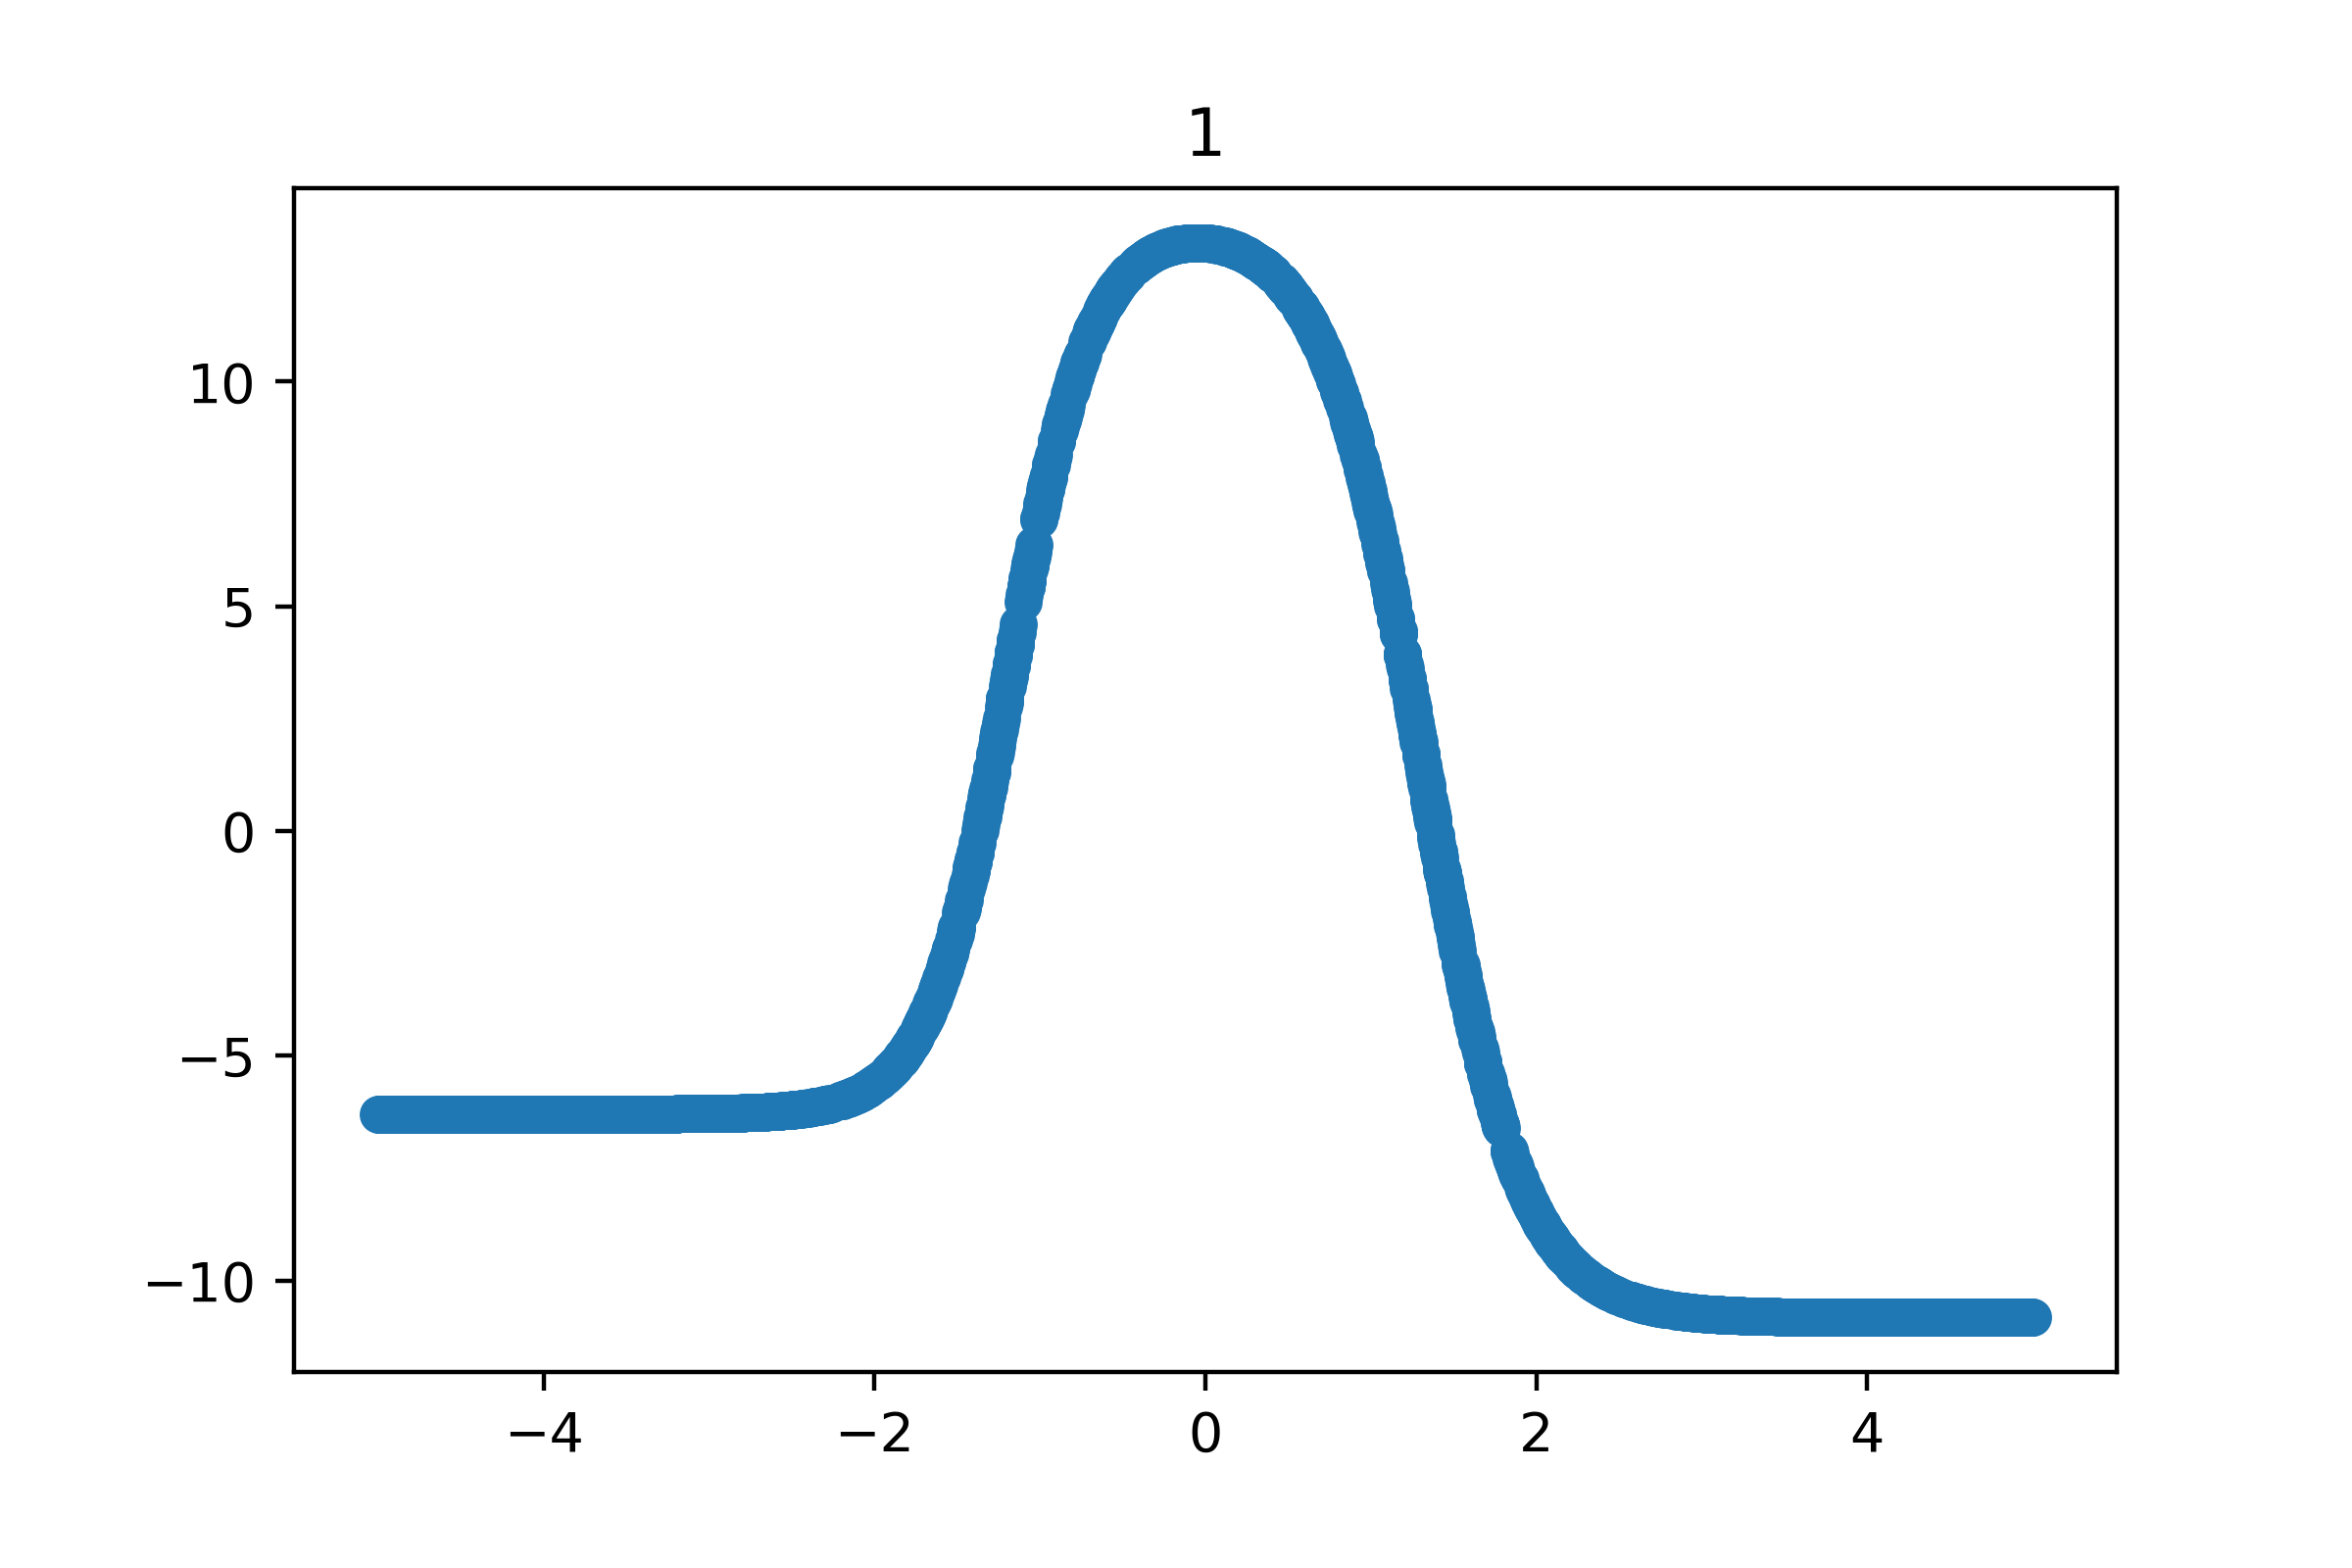
\includegraphics[width=0.22\textwidth]{fig/mnl/ci2.png}\tabularnewline
    
%     % Ellipse & 
%     % 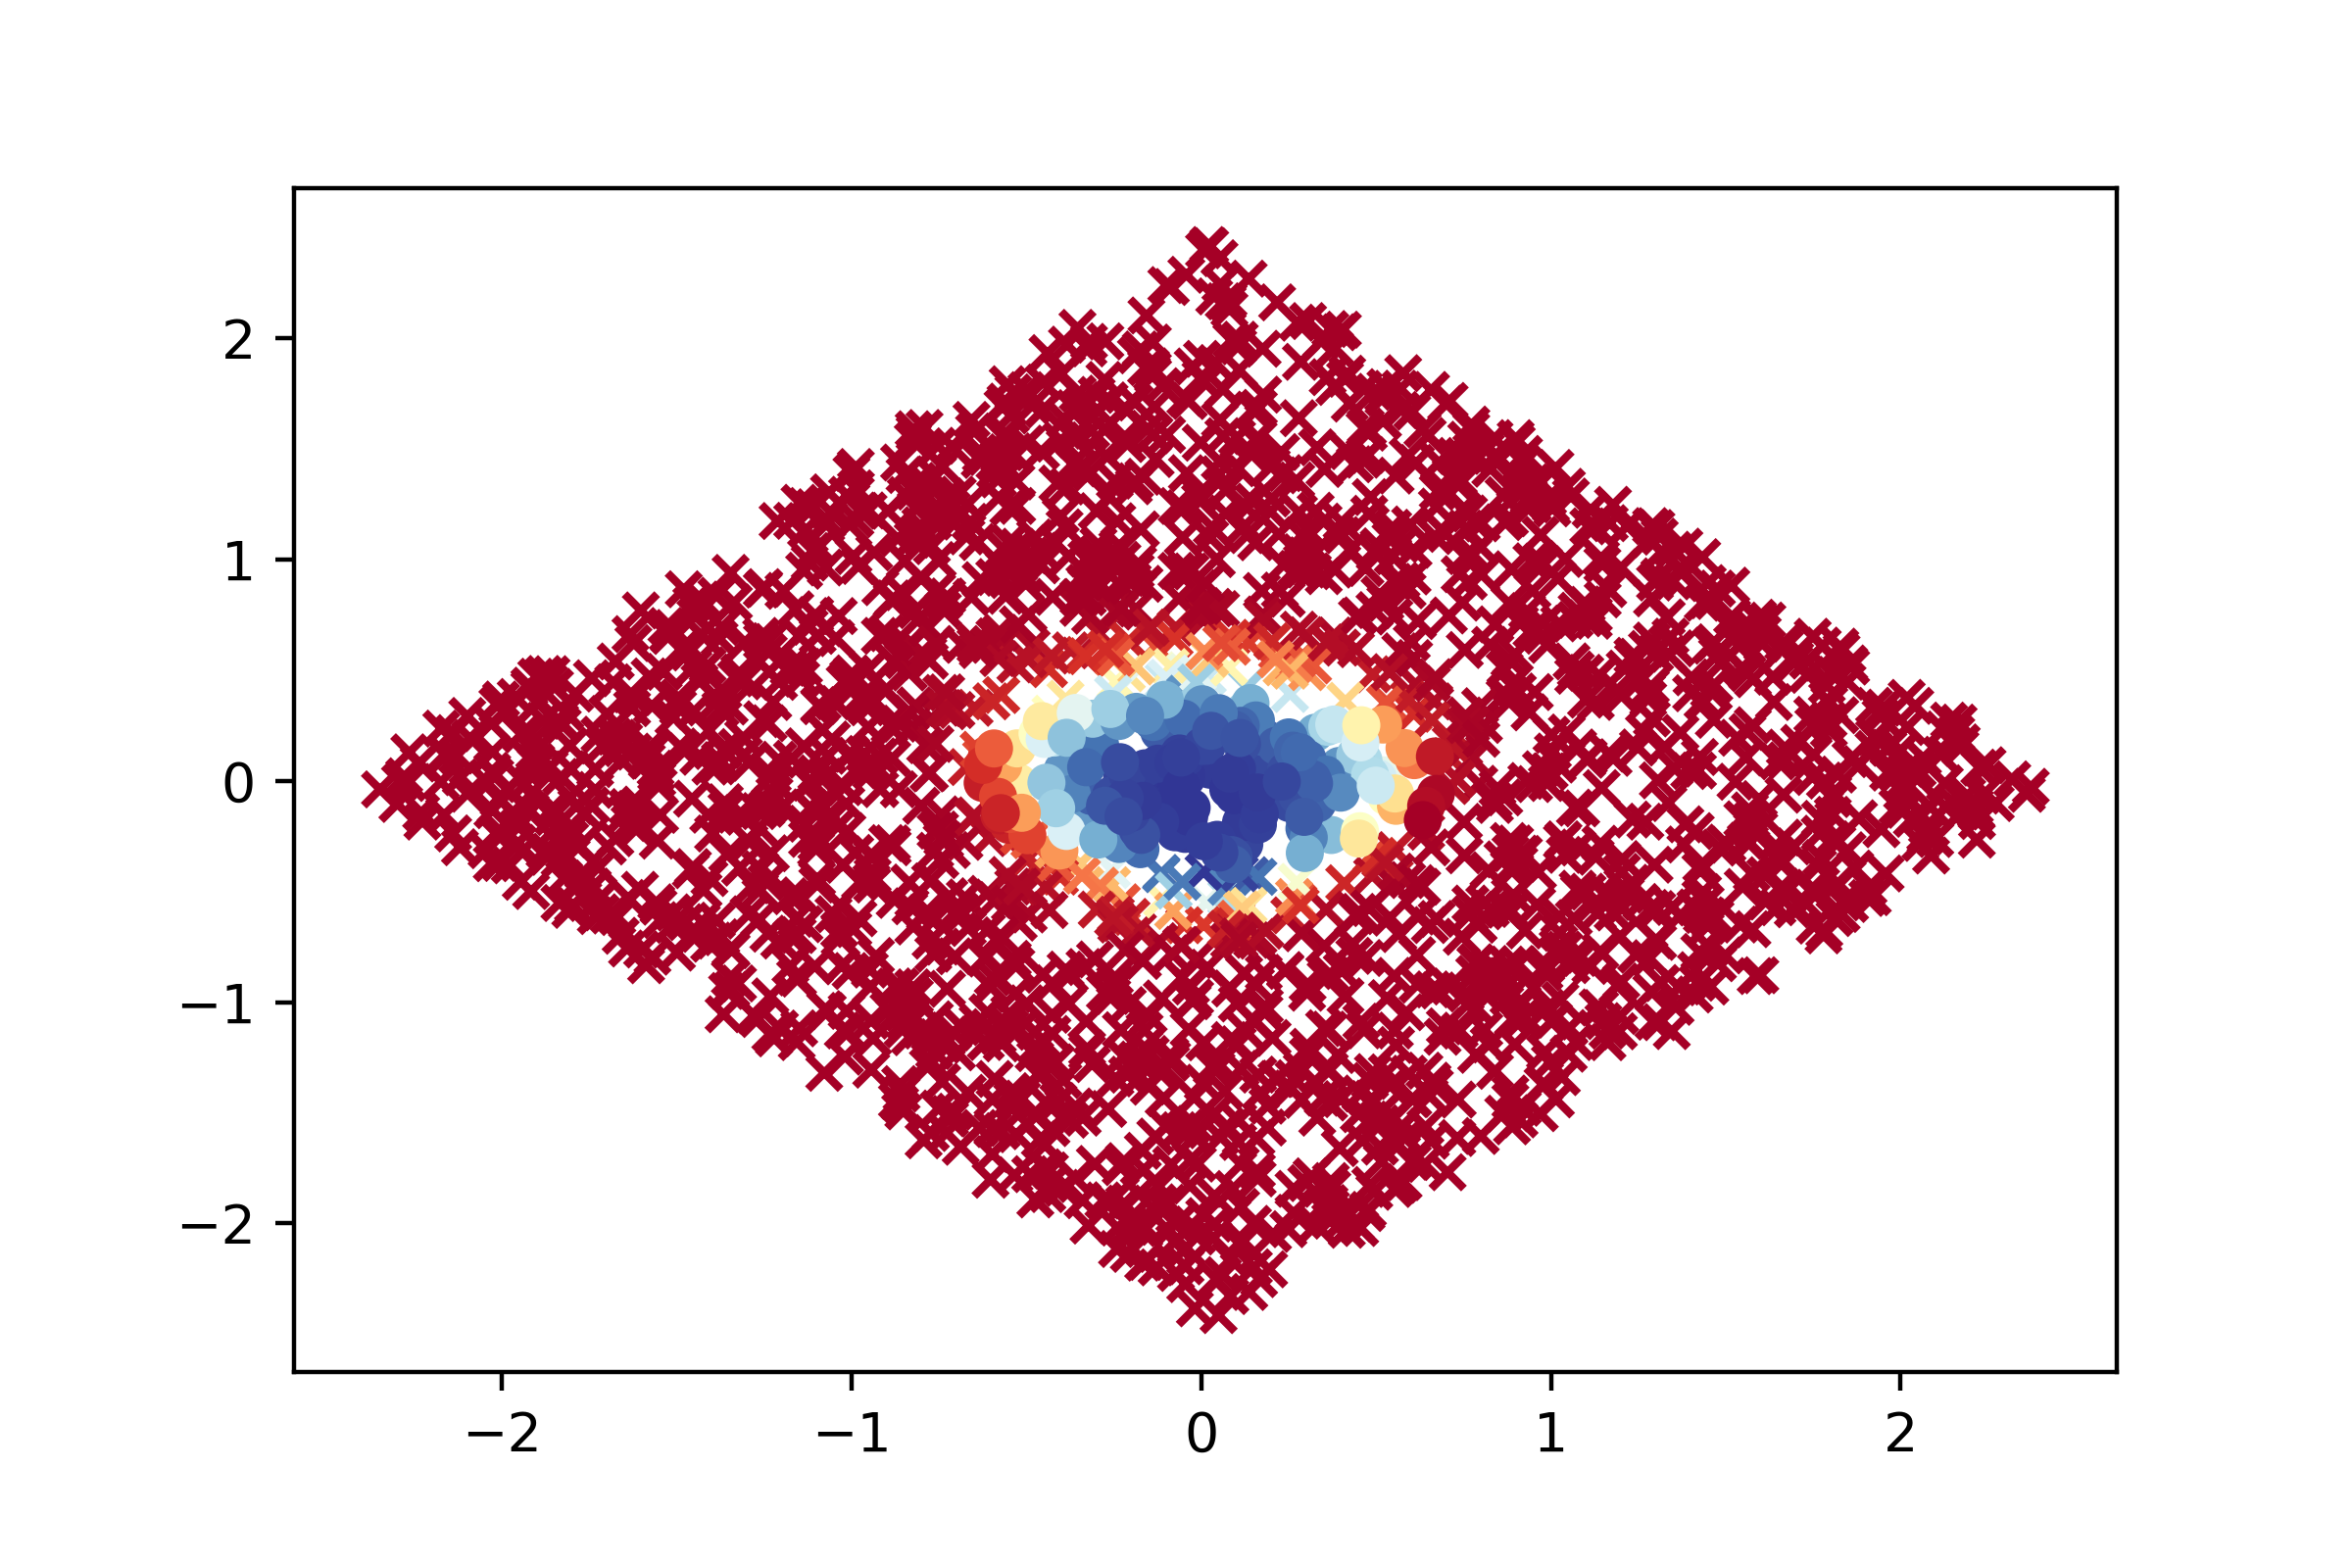
\includegraphics[width=0.22\textwidth]{fig/plt/el.png} &
%     % 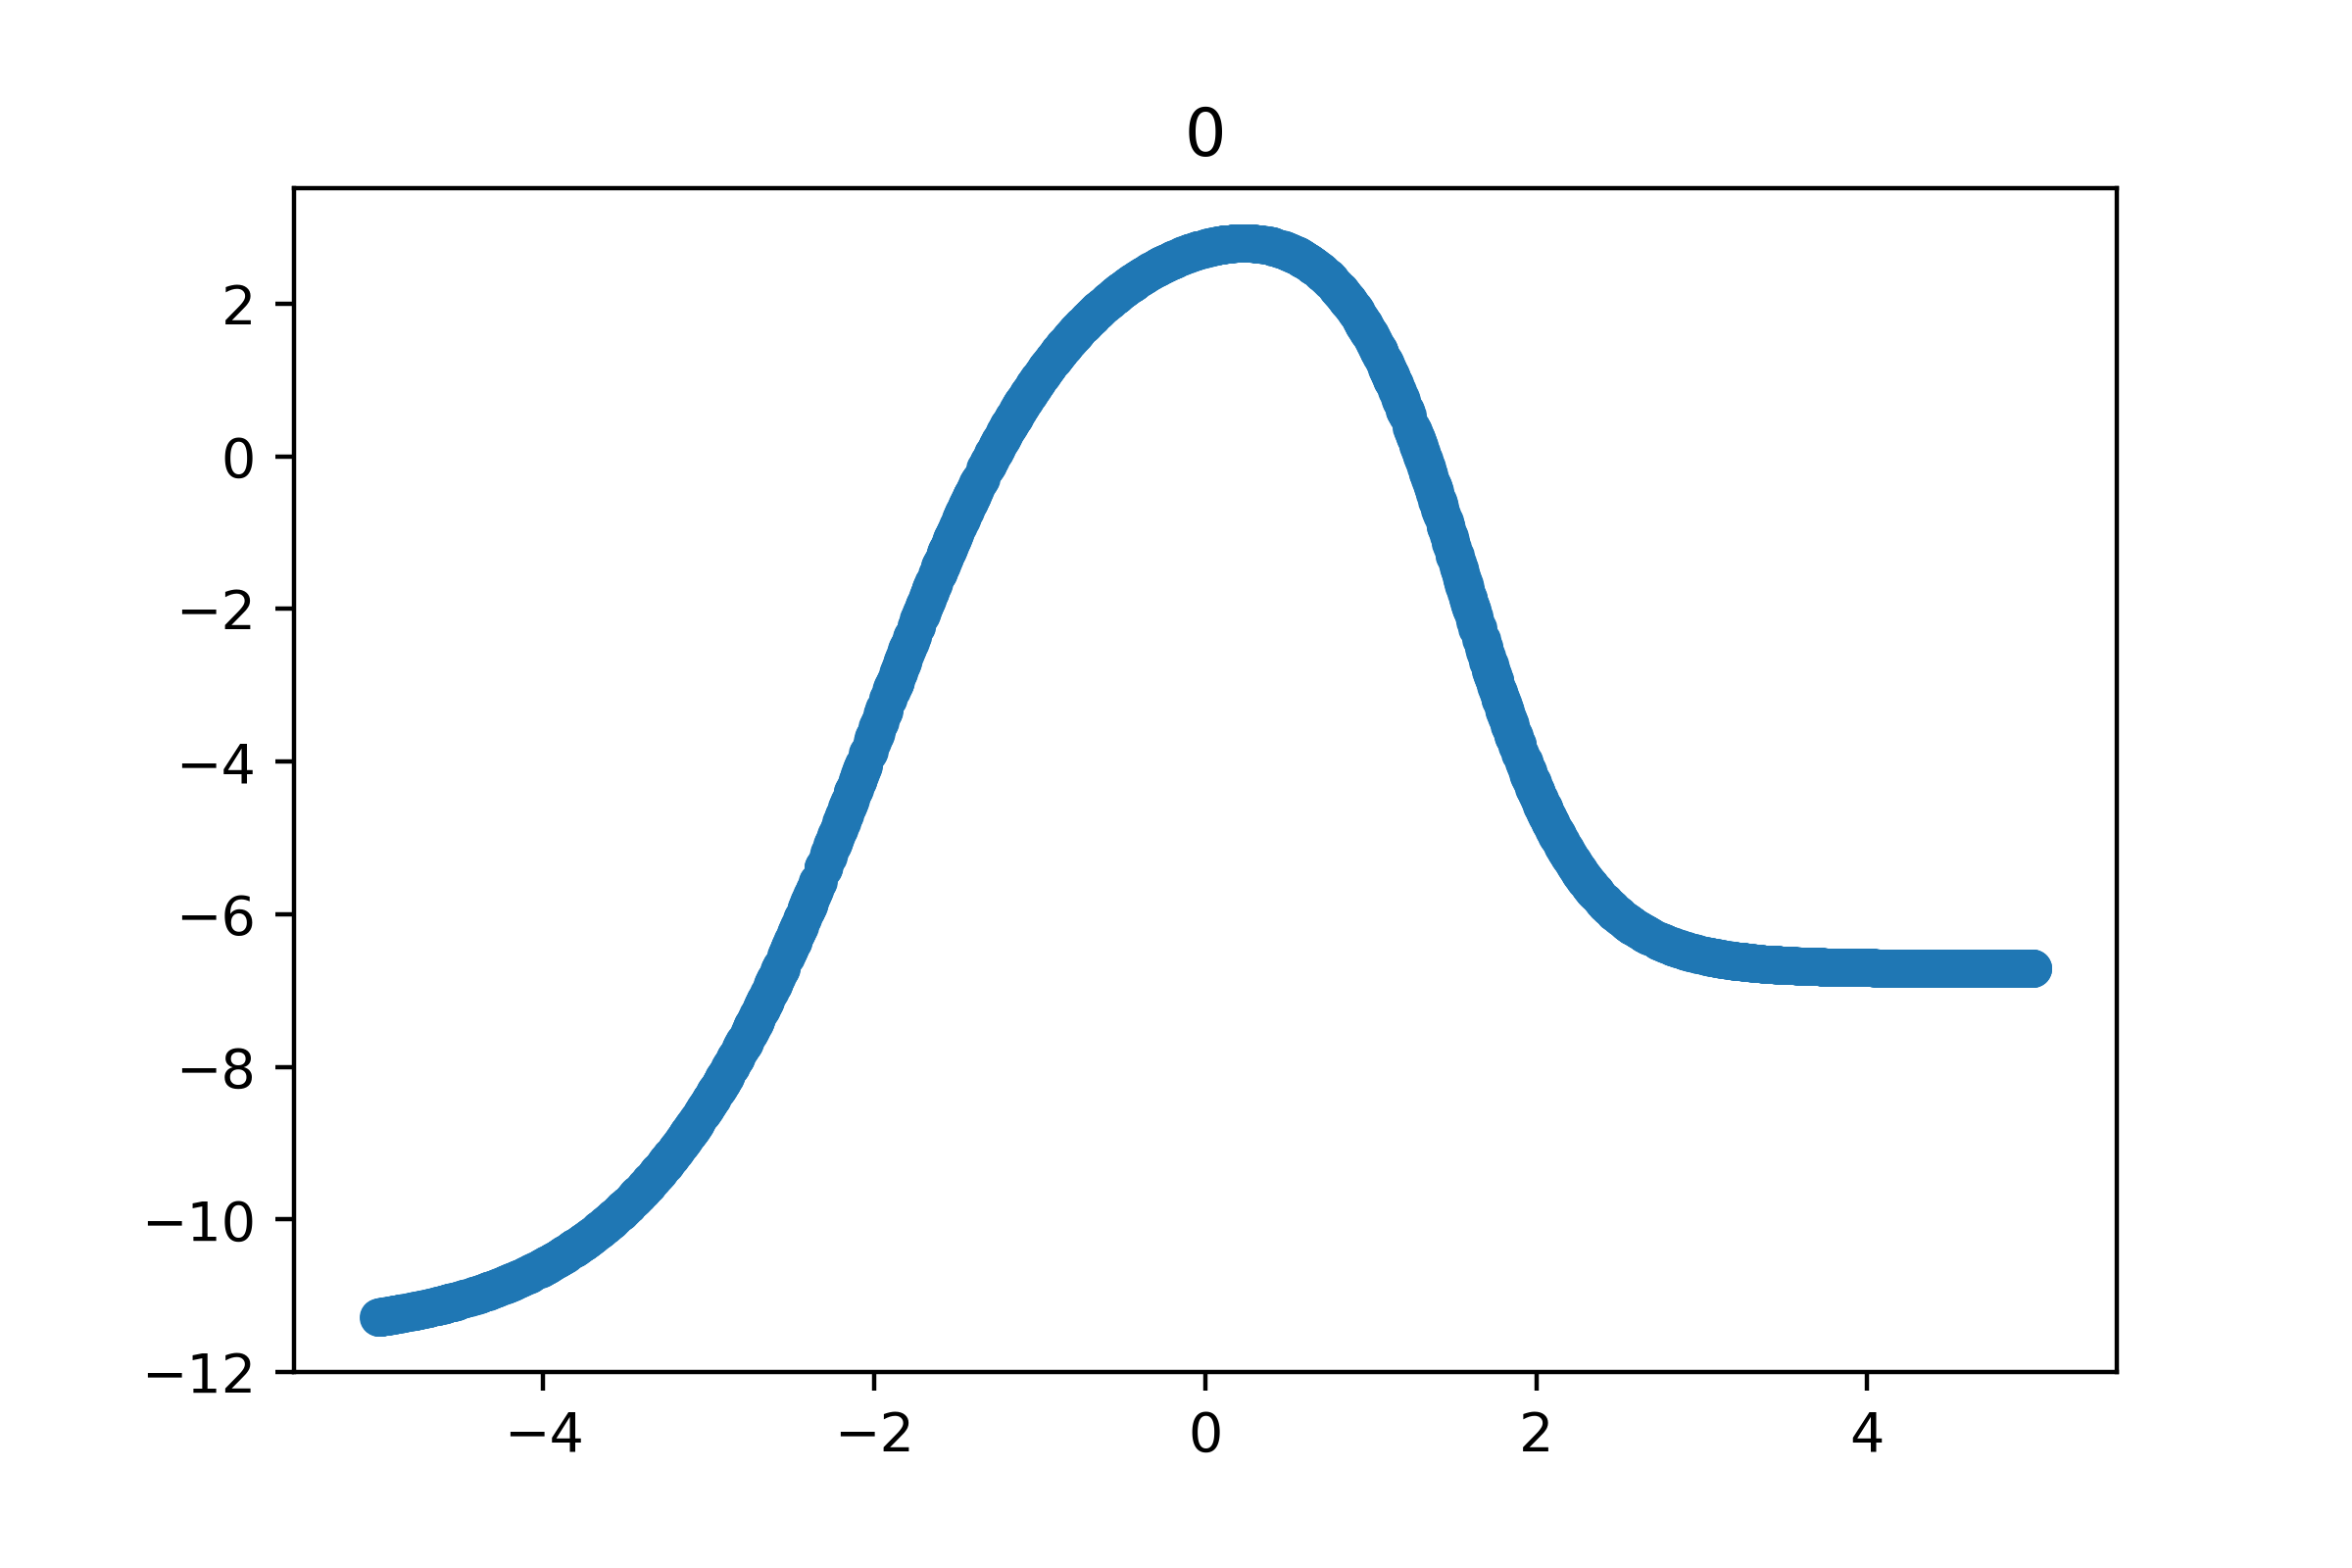
\includegraphics[width=0.22\textwidth]{fig/mnl/el1.png} &
%     % 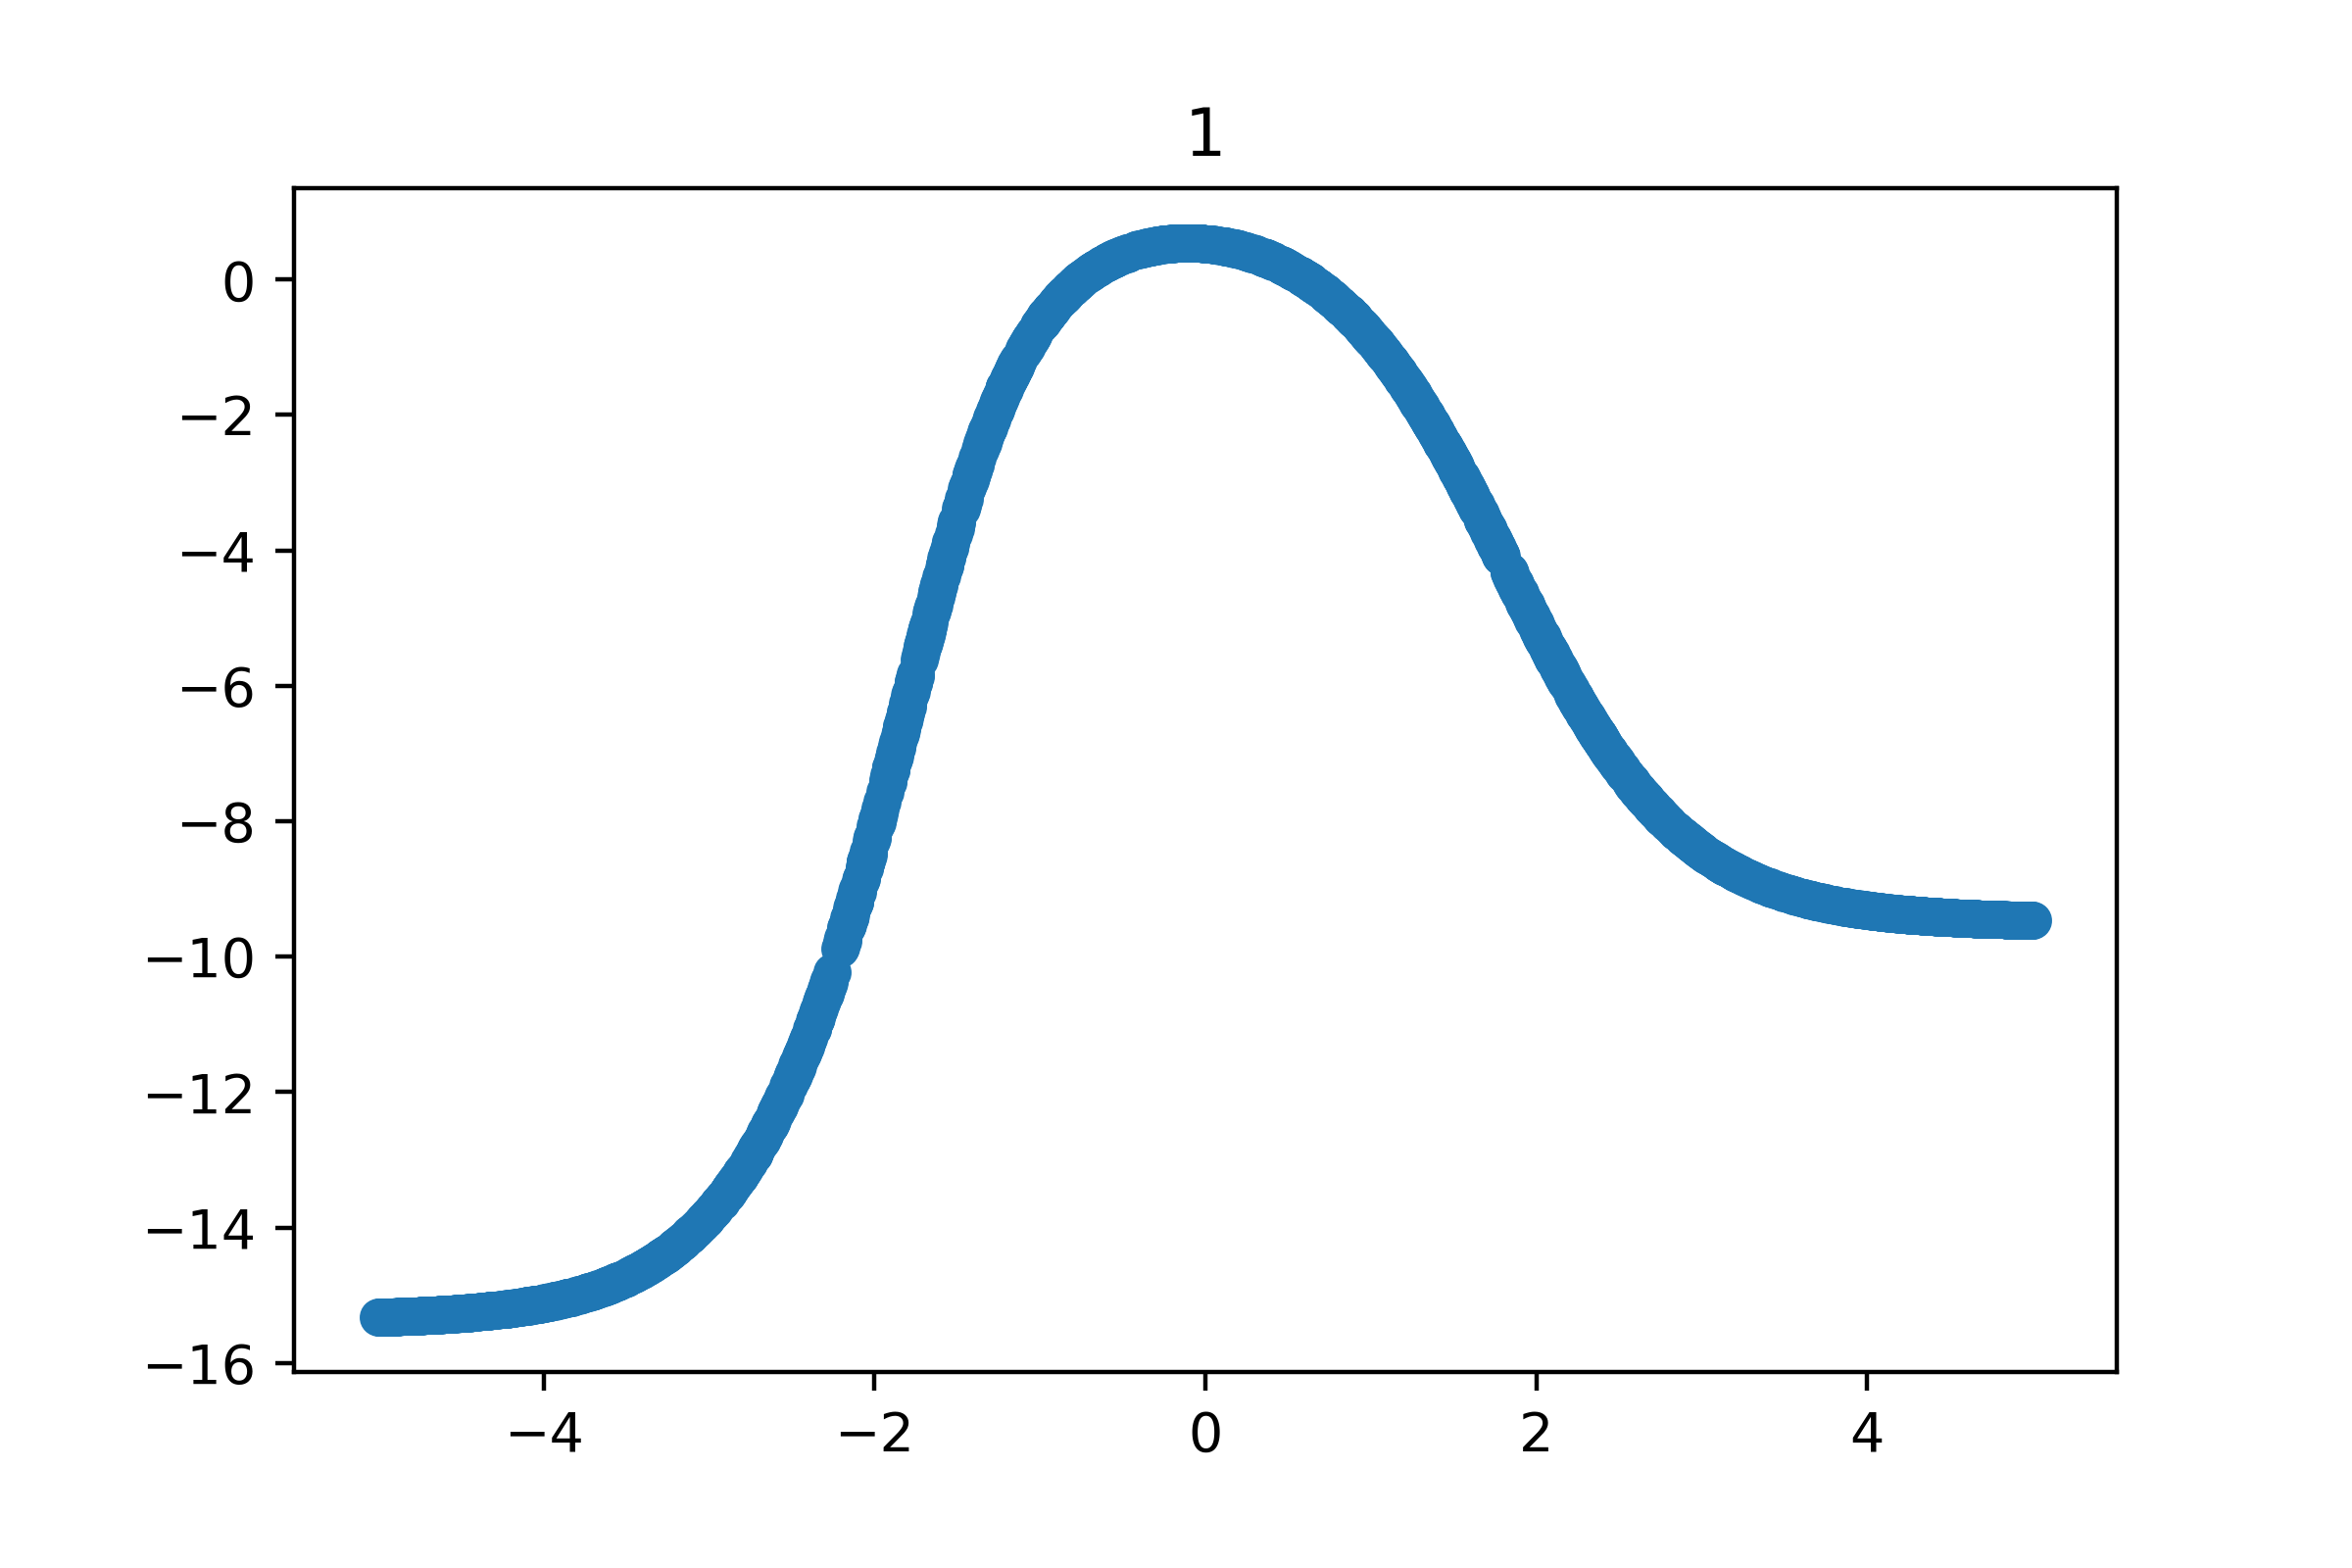
\includegraphics[width=0.22\textwidth]{fig/mnl/el2.png}\tabularnewline
    
%     % XOR & 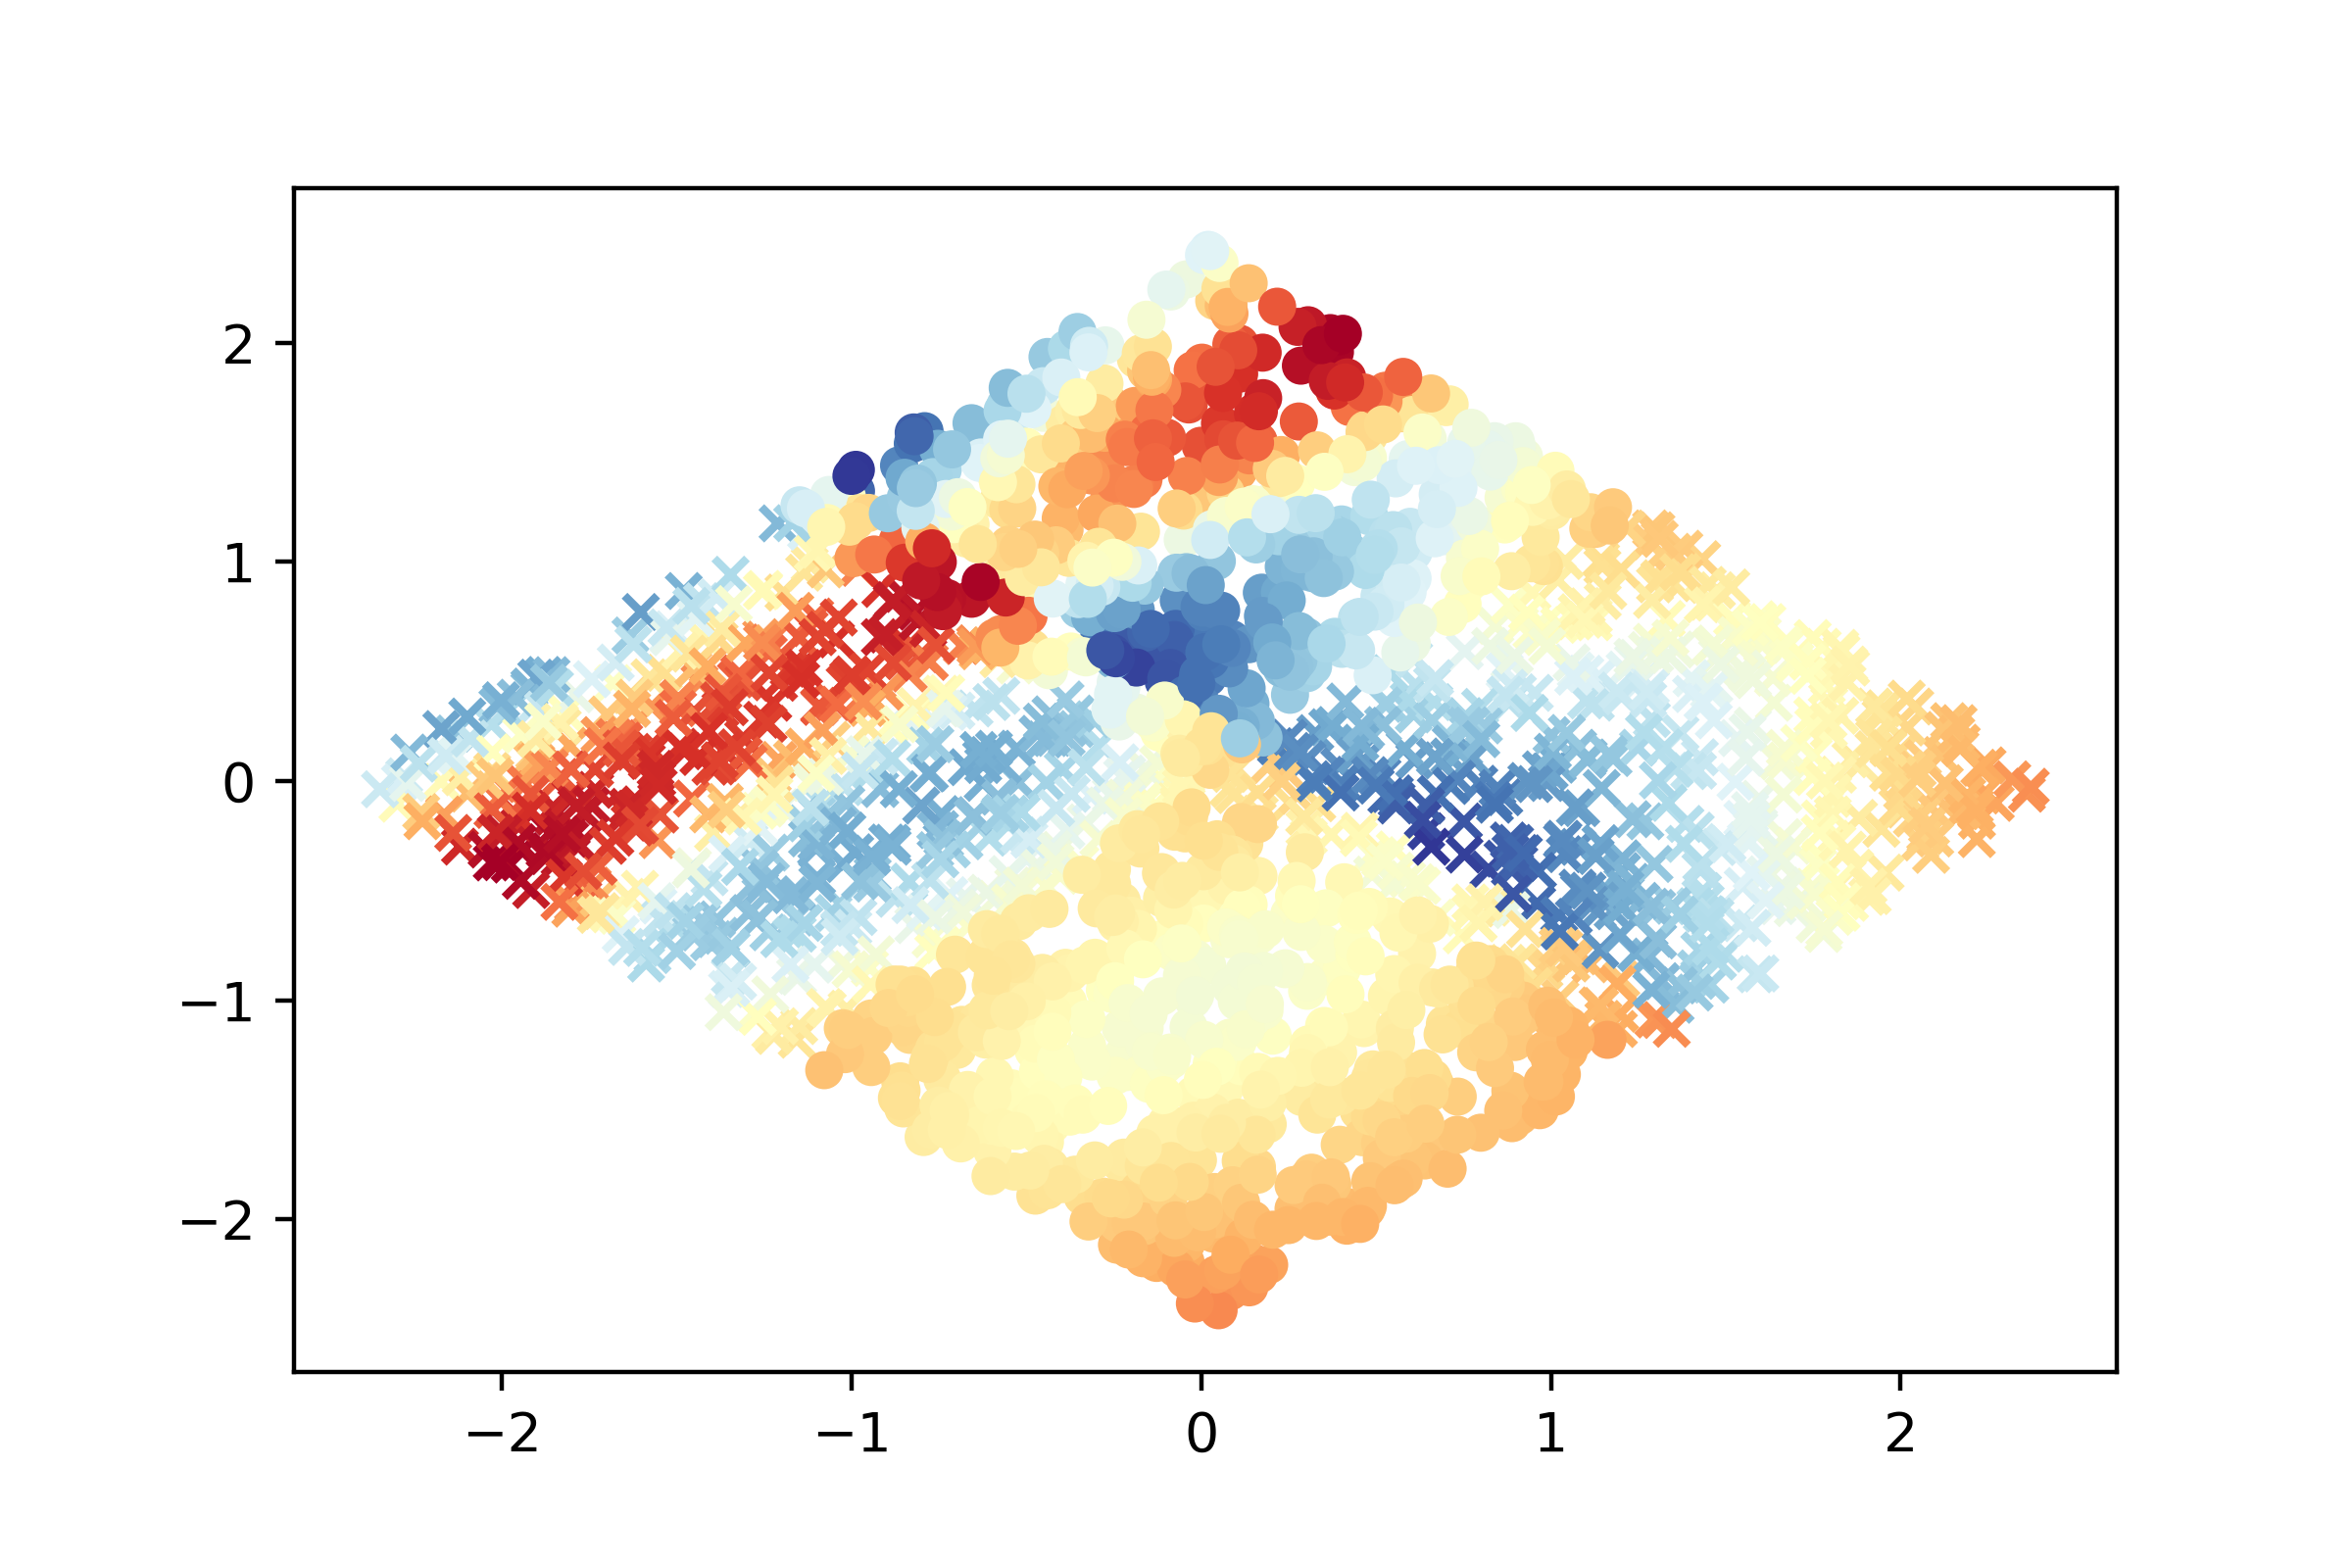
\includegraphics[width=0.22\textwidth]{fig/plt/xr.png} &
%     % 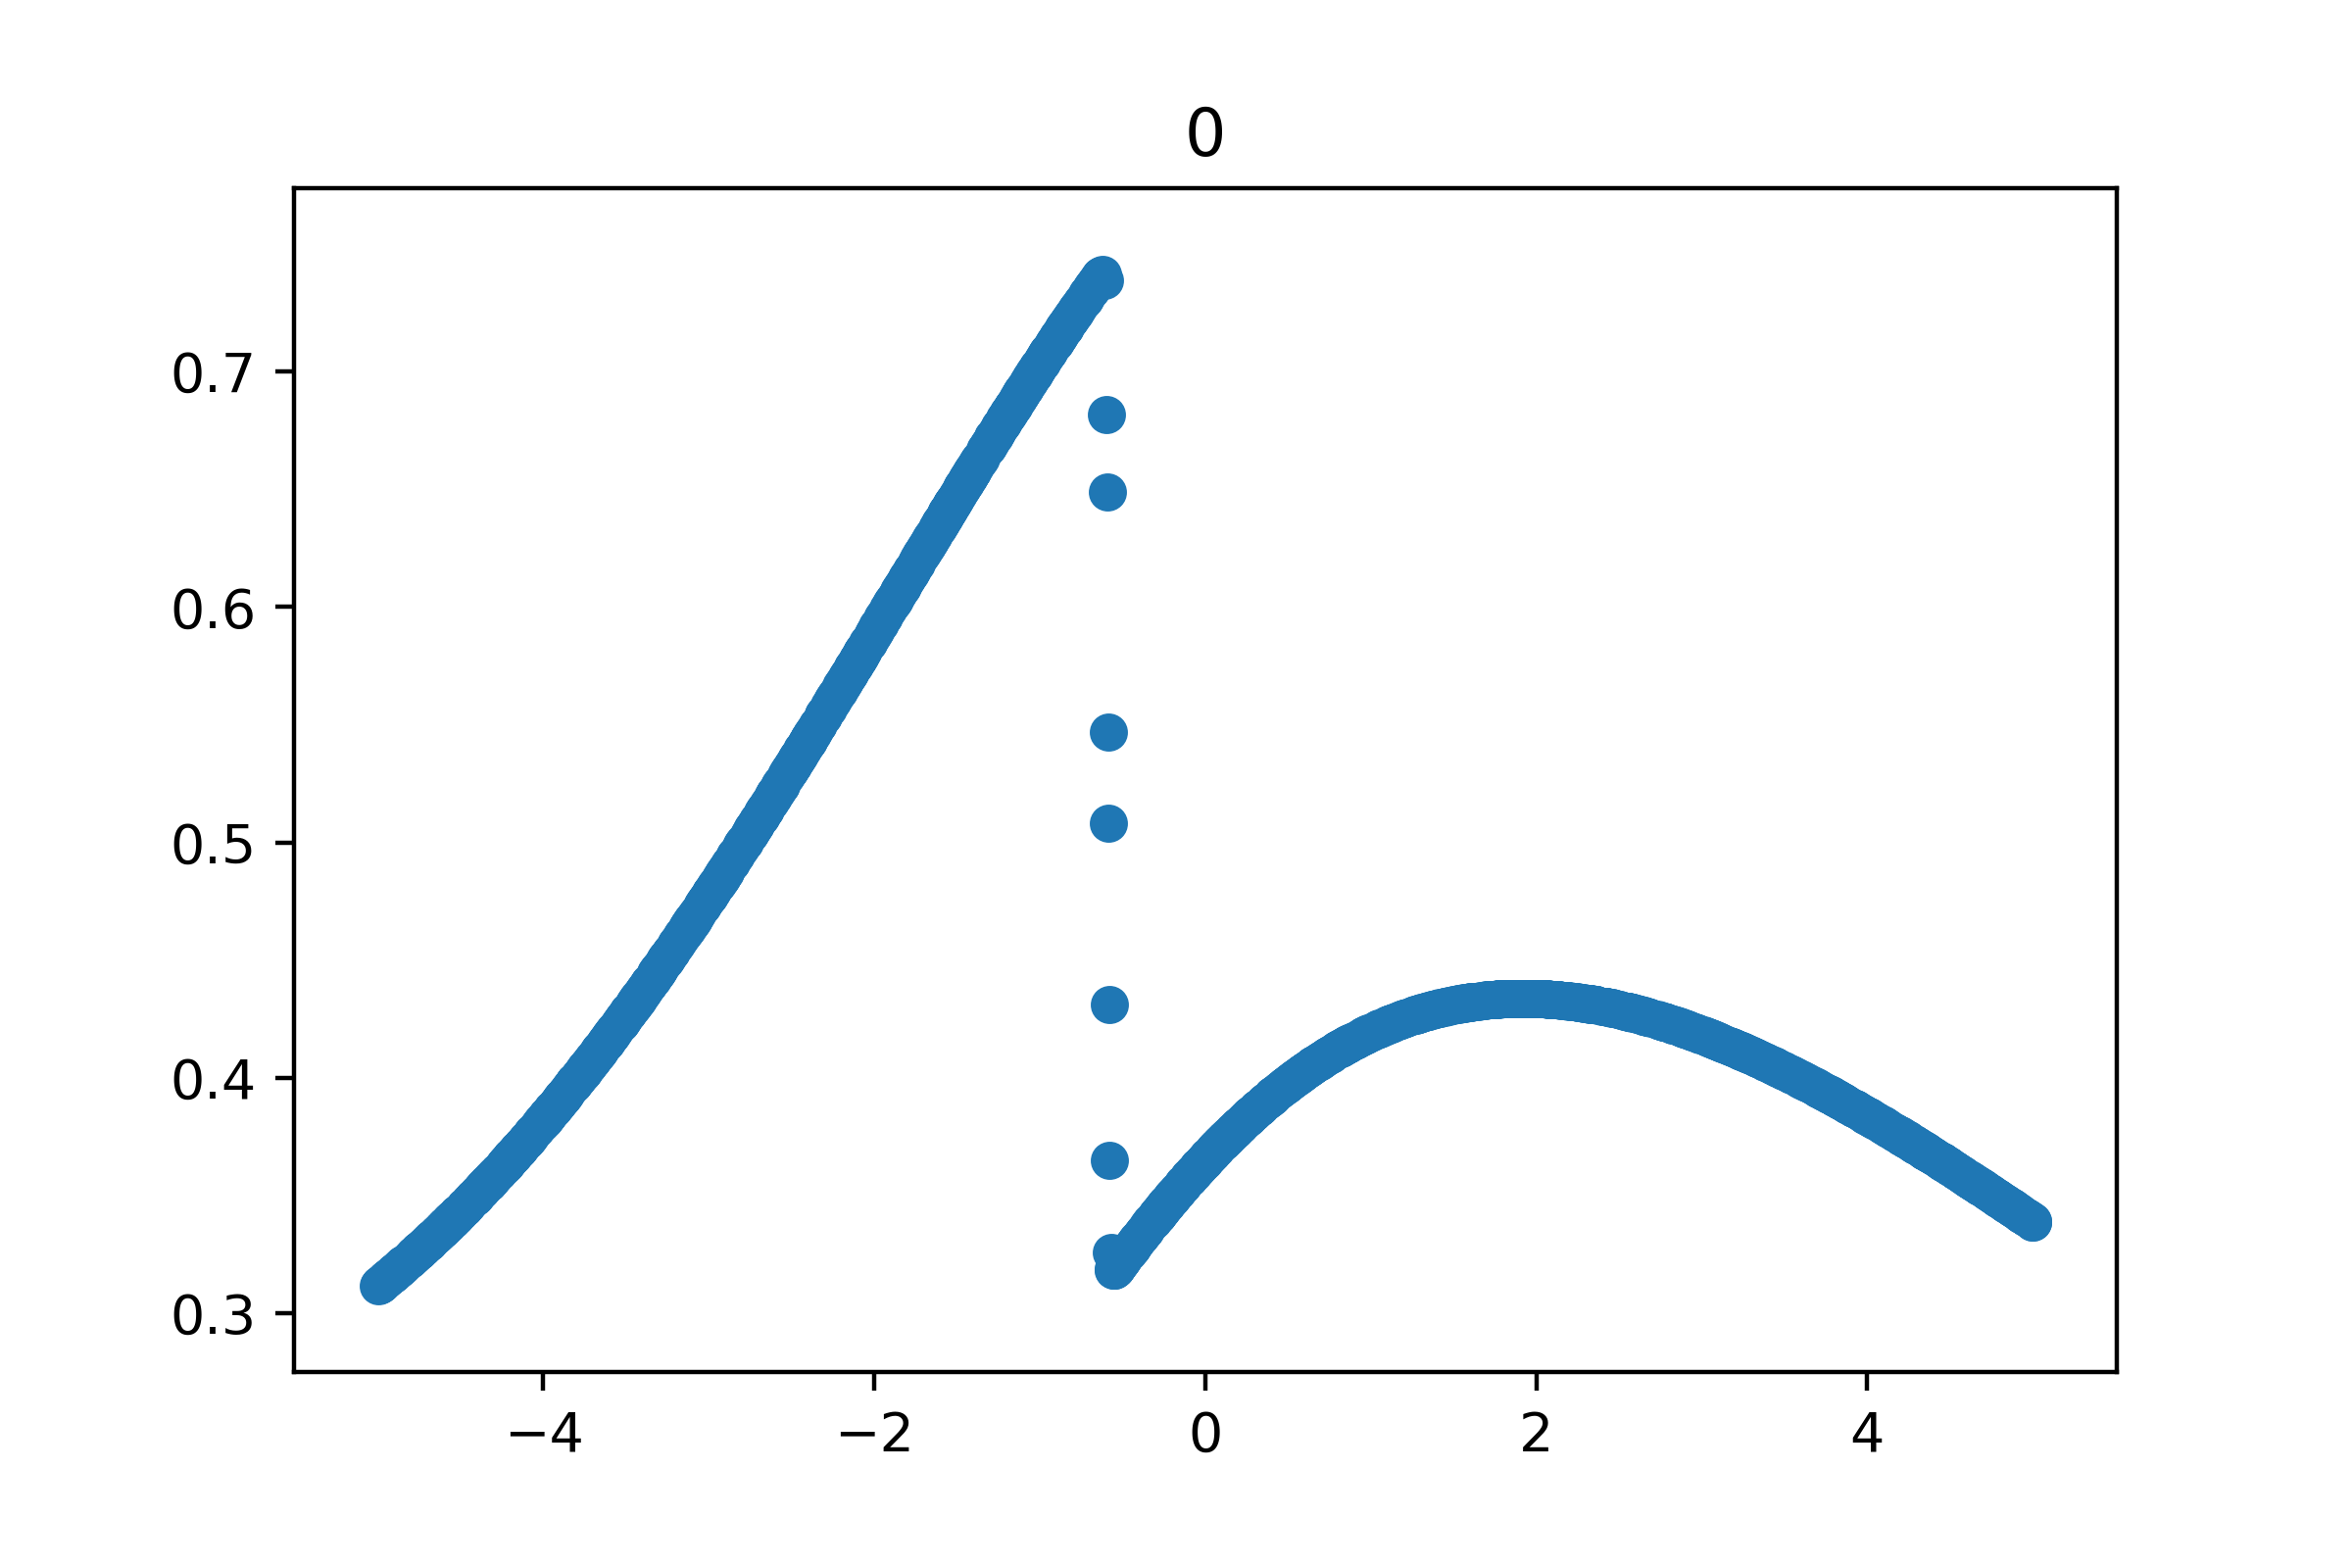
\includegraphics[width=0.22\textwidth]{fig/mnl/xr1.png} &
%     % 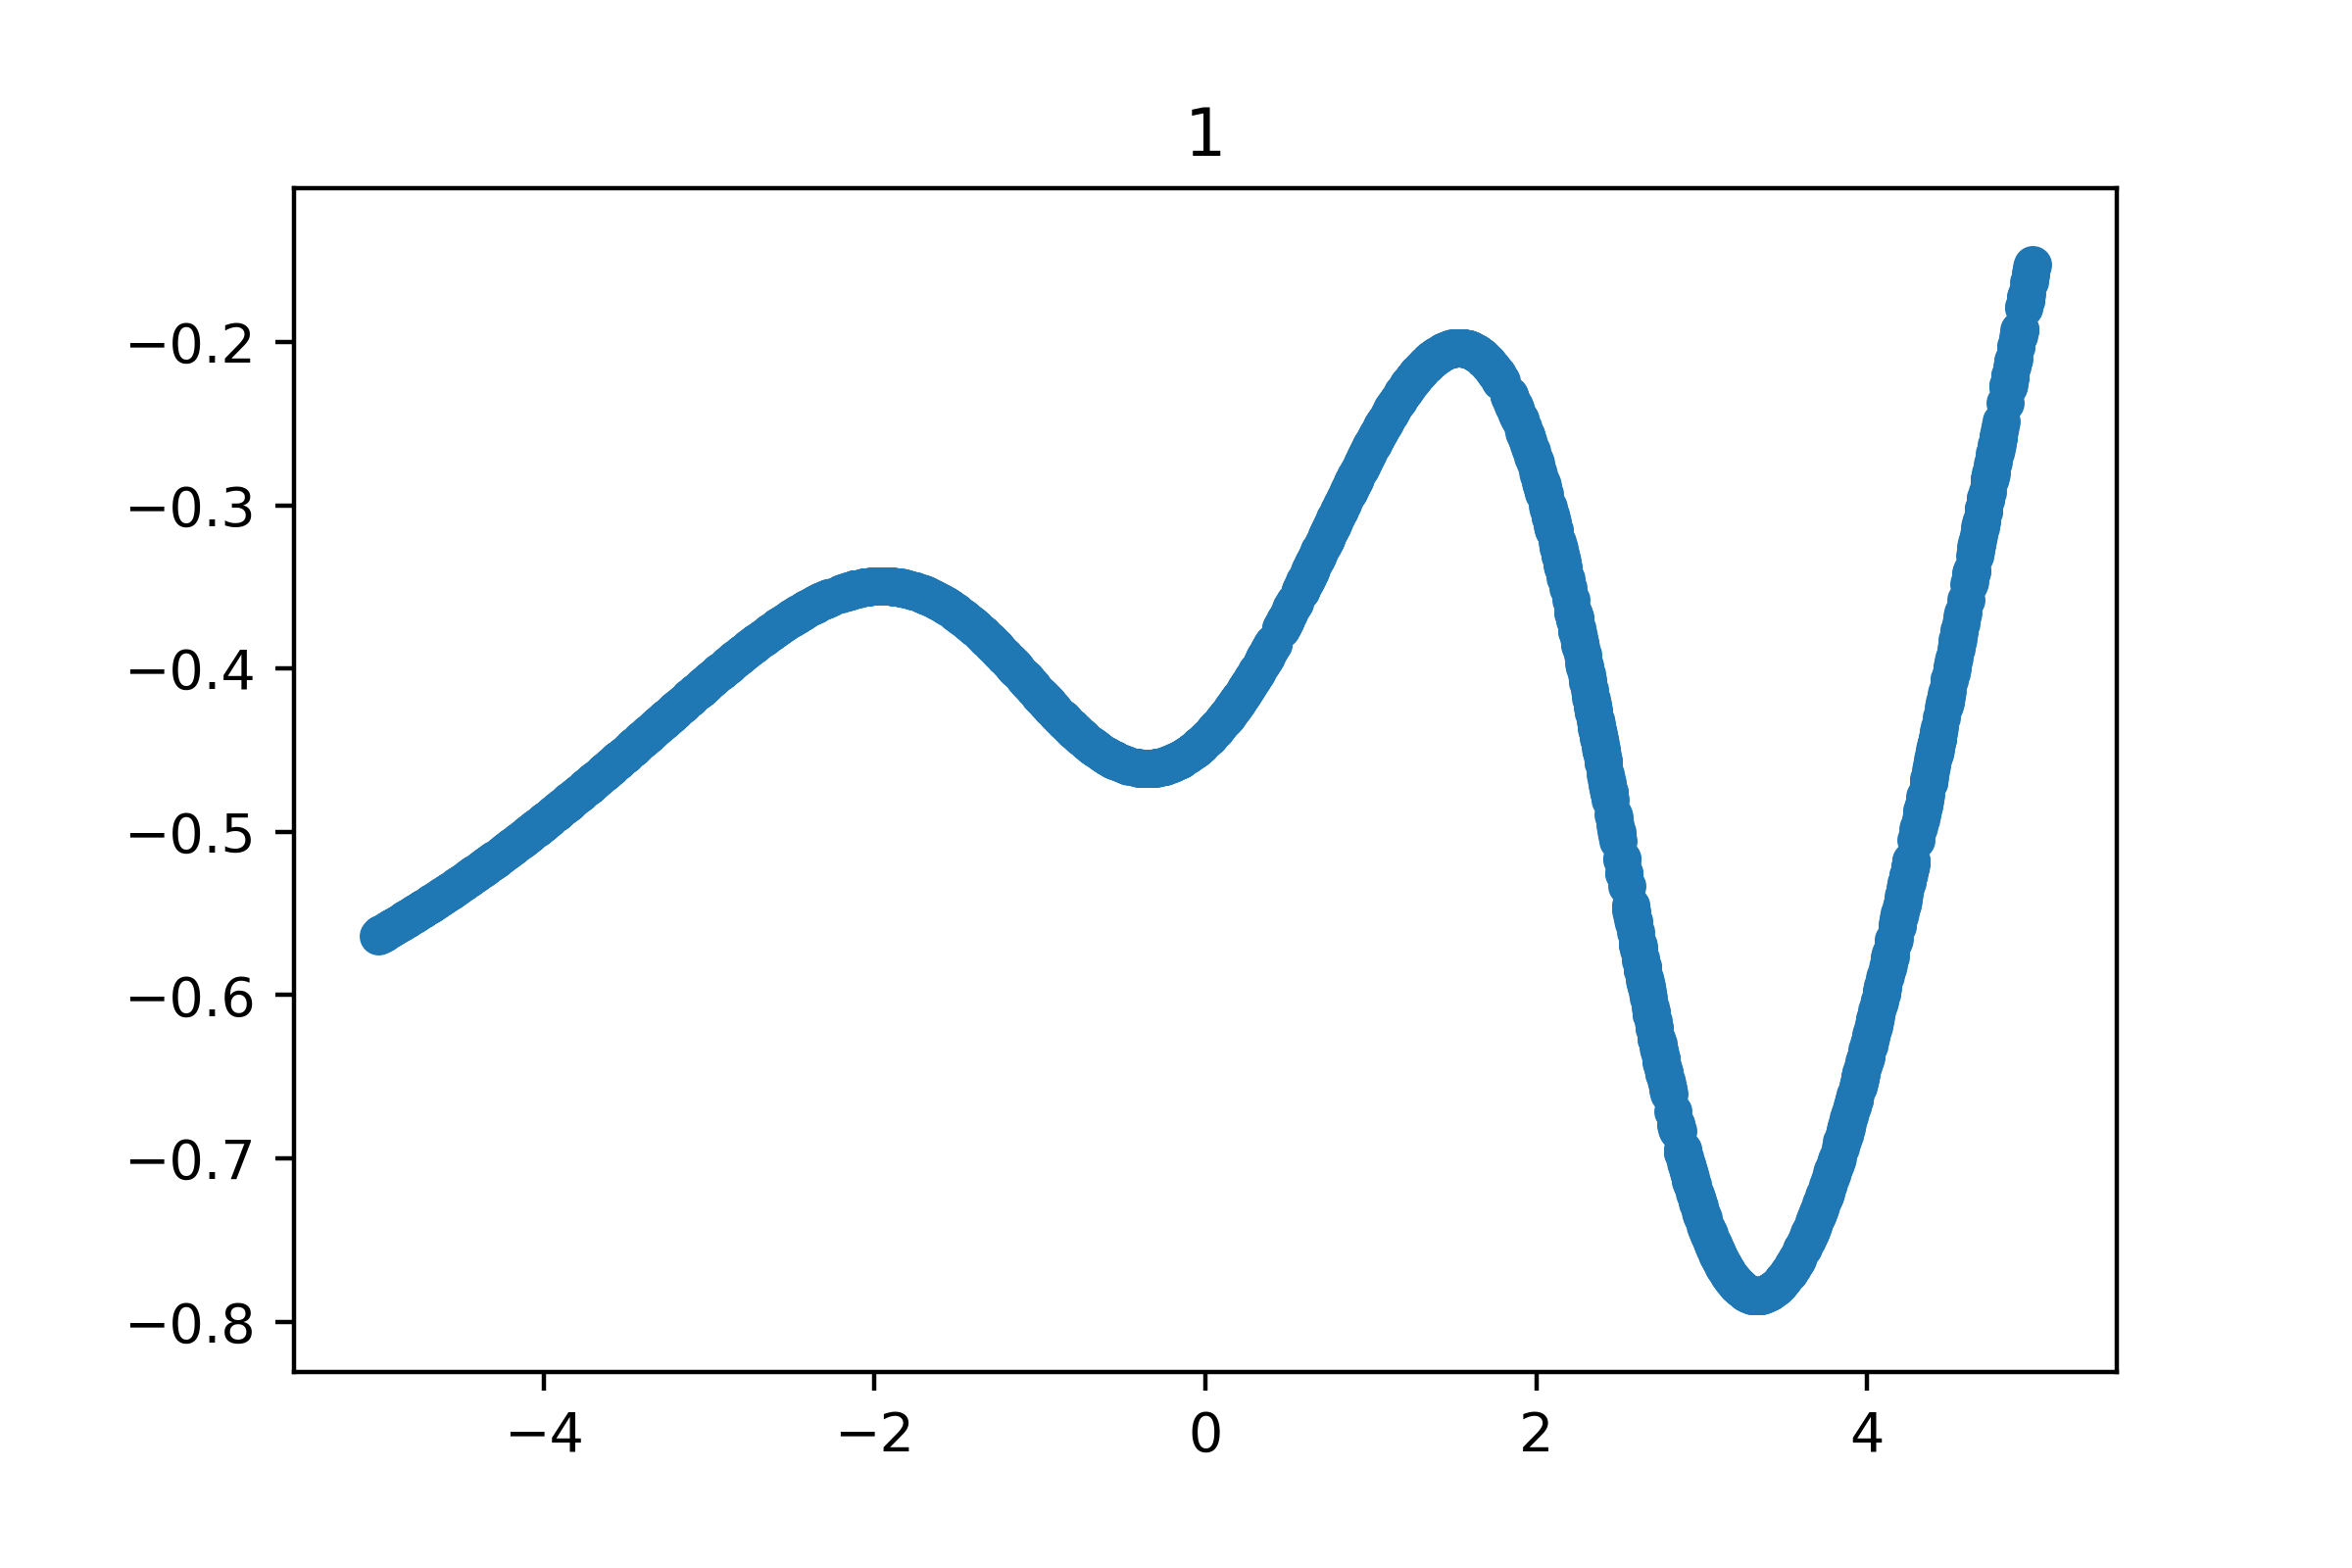
\includegraphics[width=0.22\textwidth]{fig/mnl/xr2.png}\tabularnewline

%     \bottomrule
    
%     \caption{Two-dimensional principle components plot representing the dataset. X's are true negatives and O's are true positives. Colors represent the network prediction, with blue being positive, red being negative, and yellow being neutral.}

% \end{longtable}





% \begin{longtable}[]{@{}lcc@{}}

%     \toprule
%     Dataset & Marginal 1 & Marginal 2%
%     \tabularnewline
%     \midrule
%     \endhead

%     Cancer &
%     %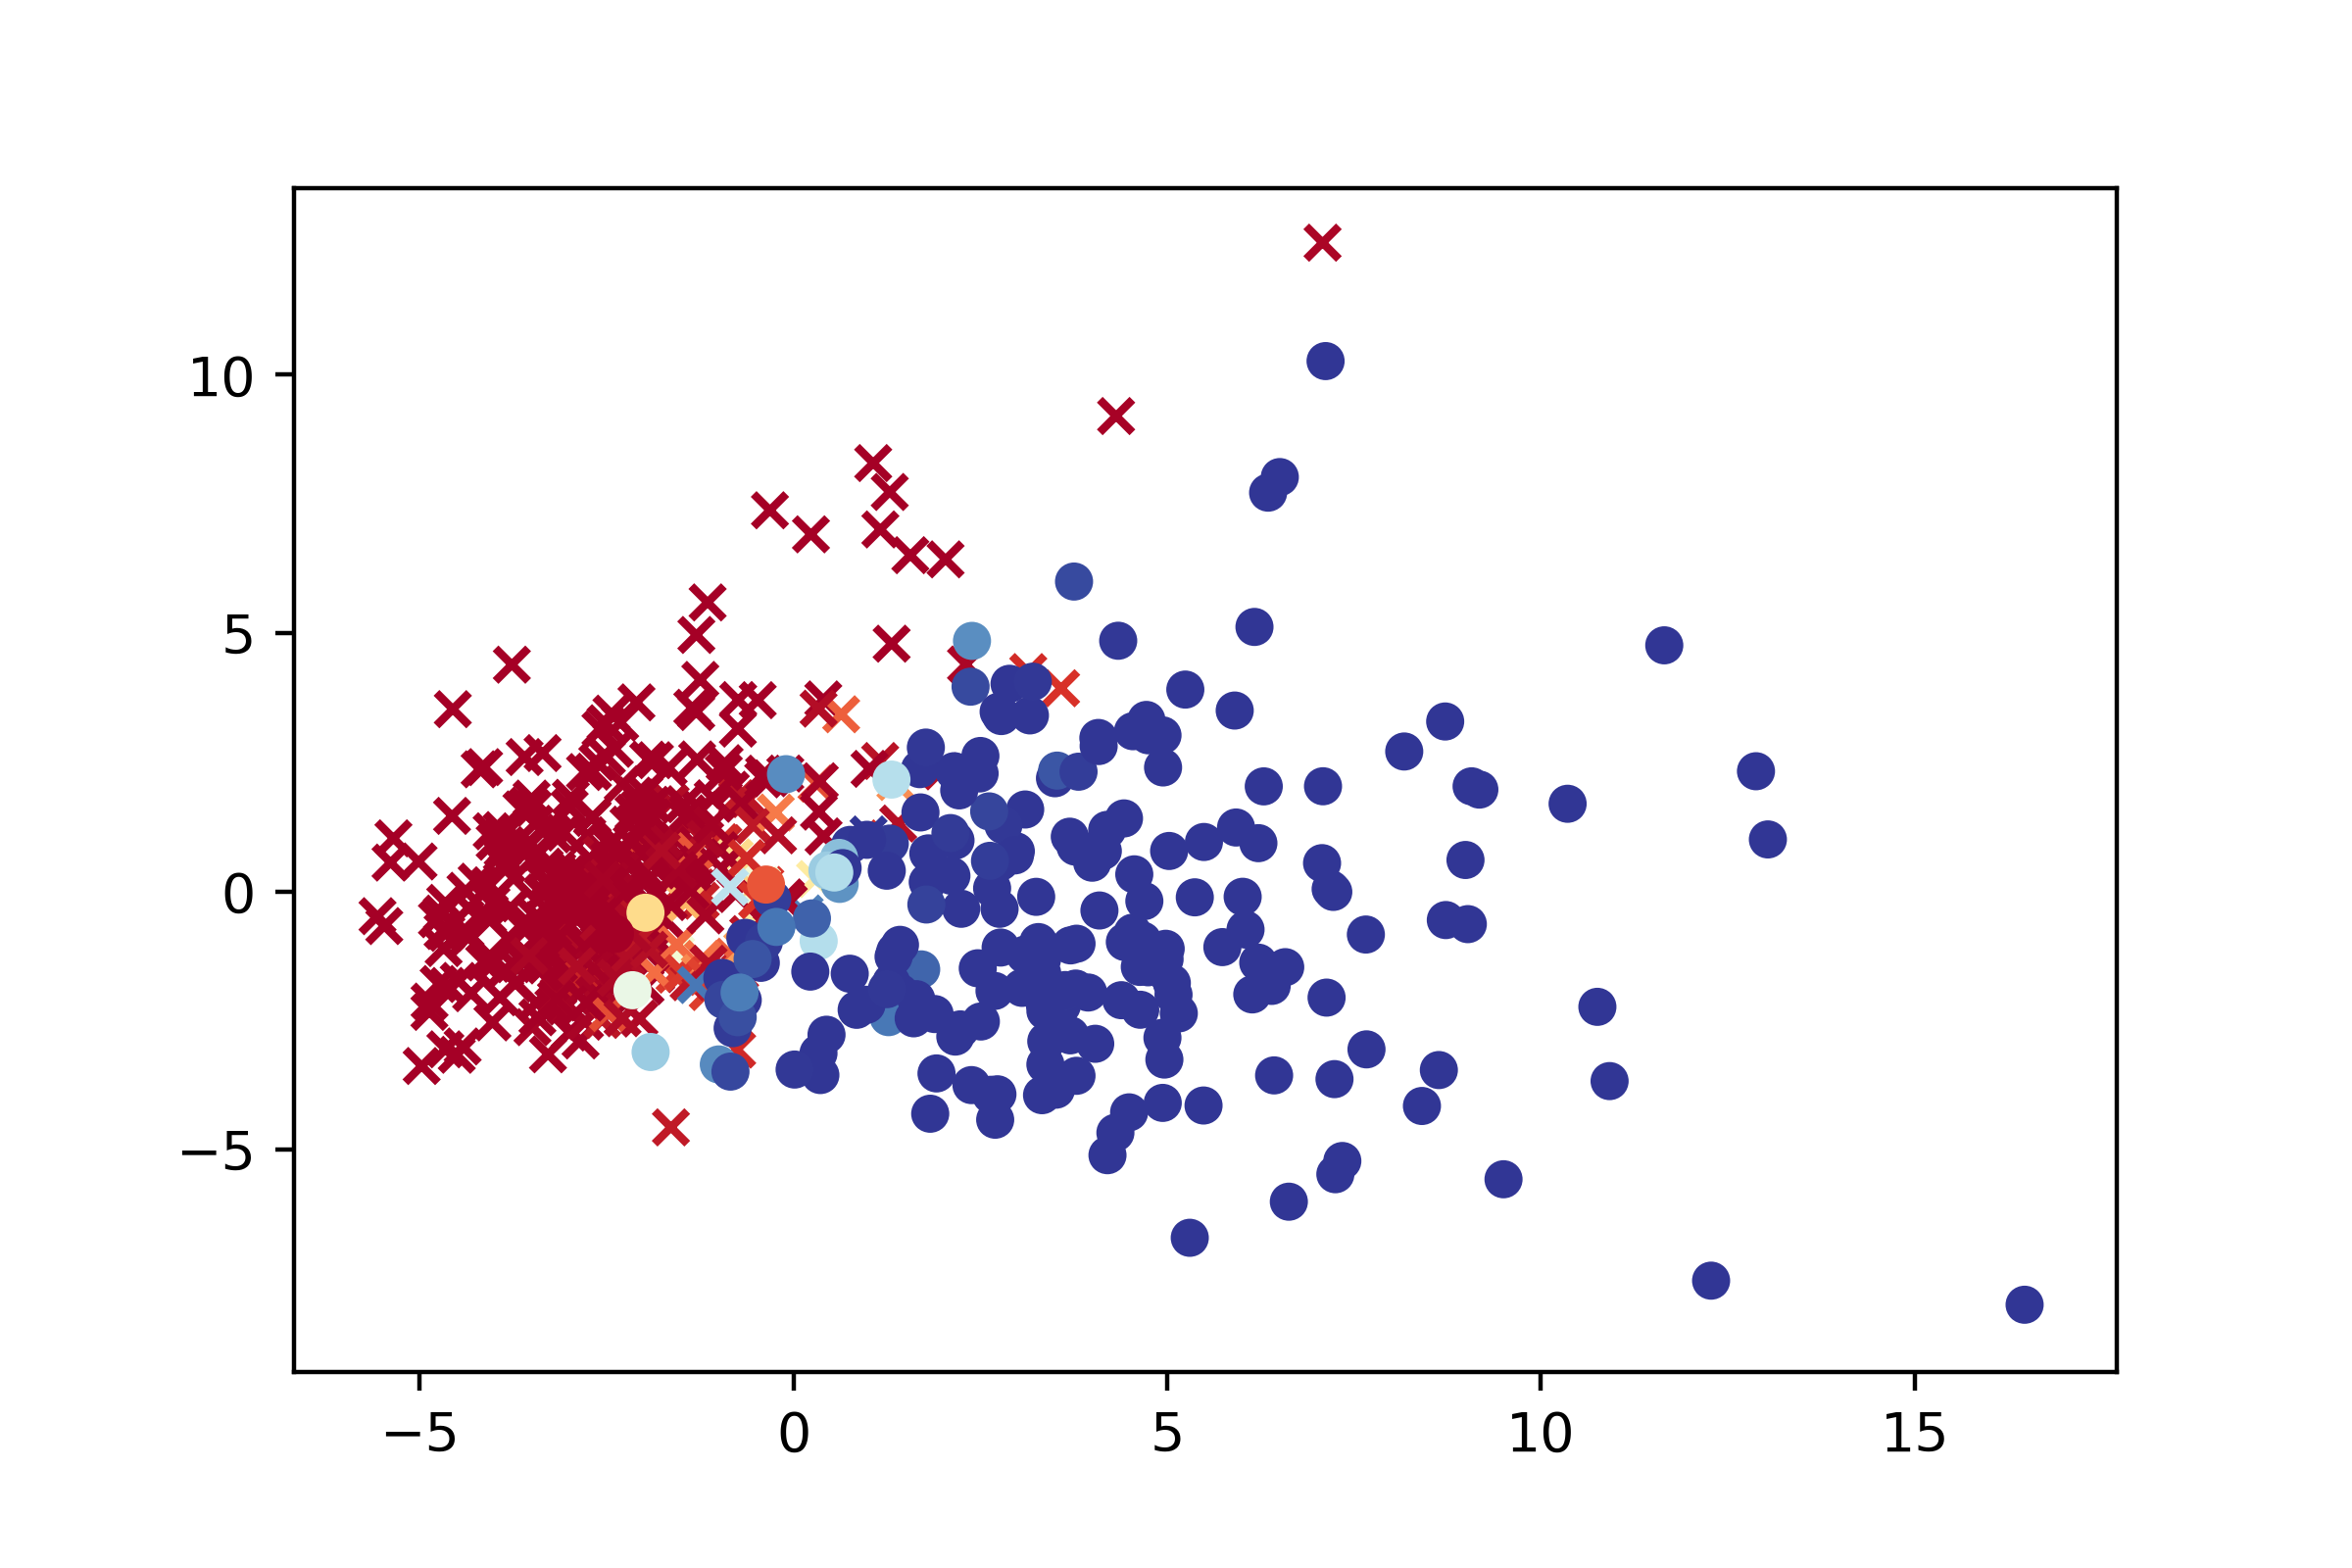
\includegraphics[width=0.22\textwidth]{fig/plt/bc.png} &
%     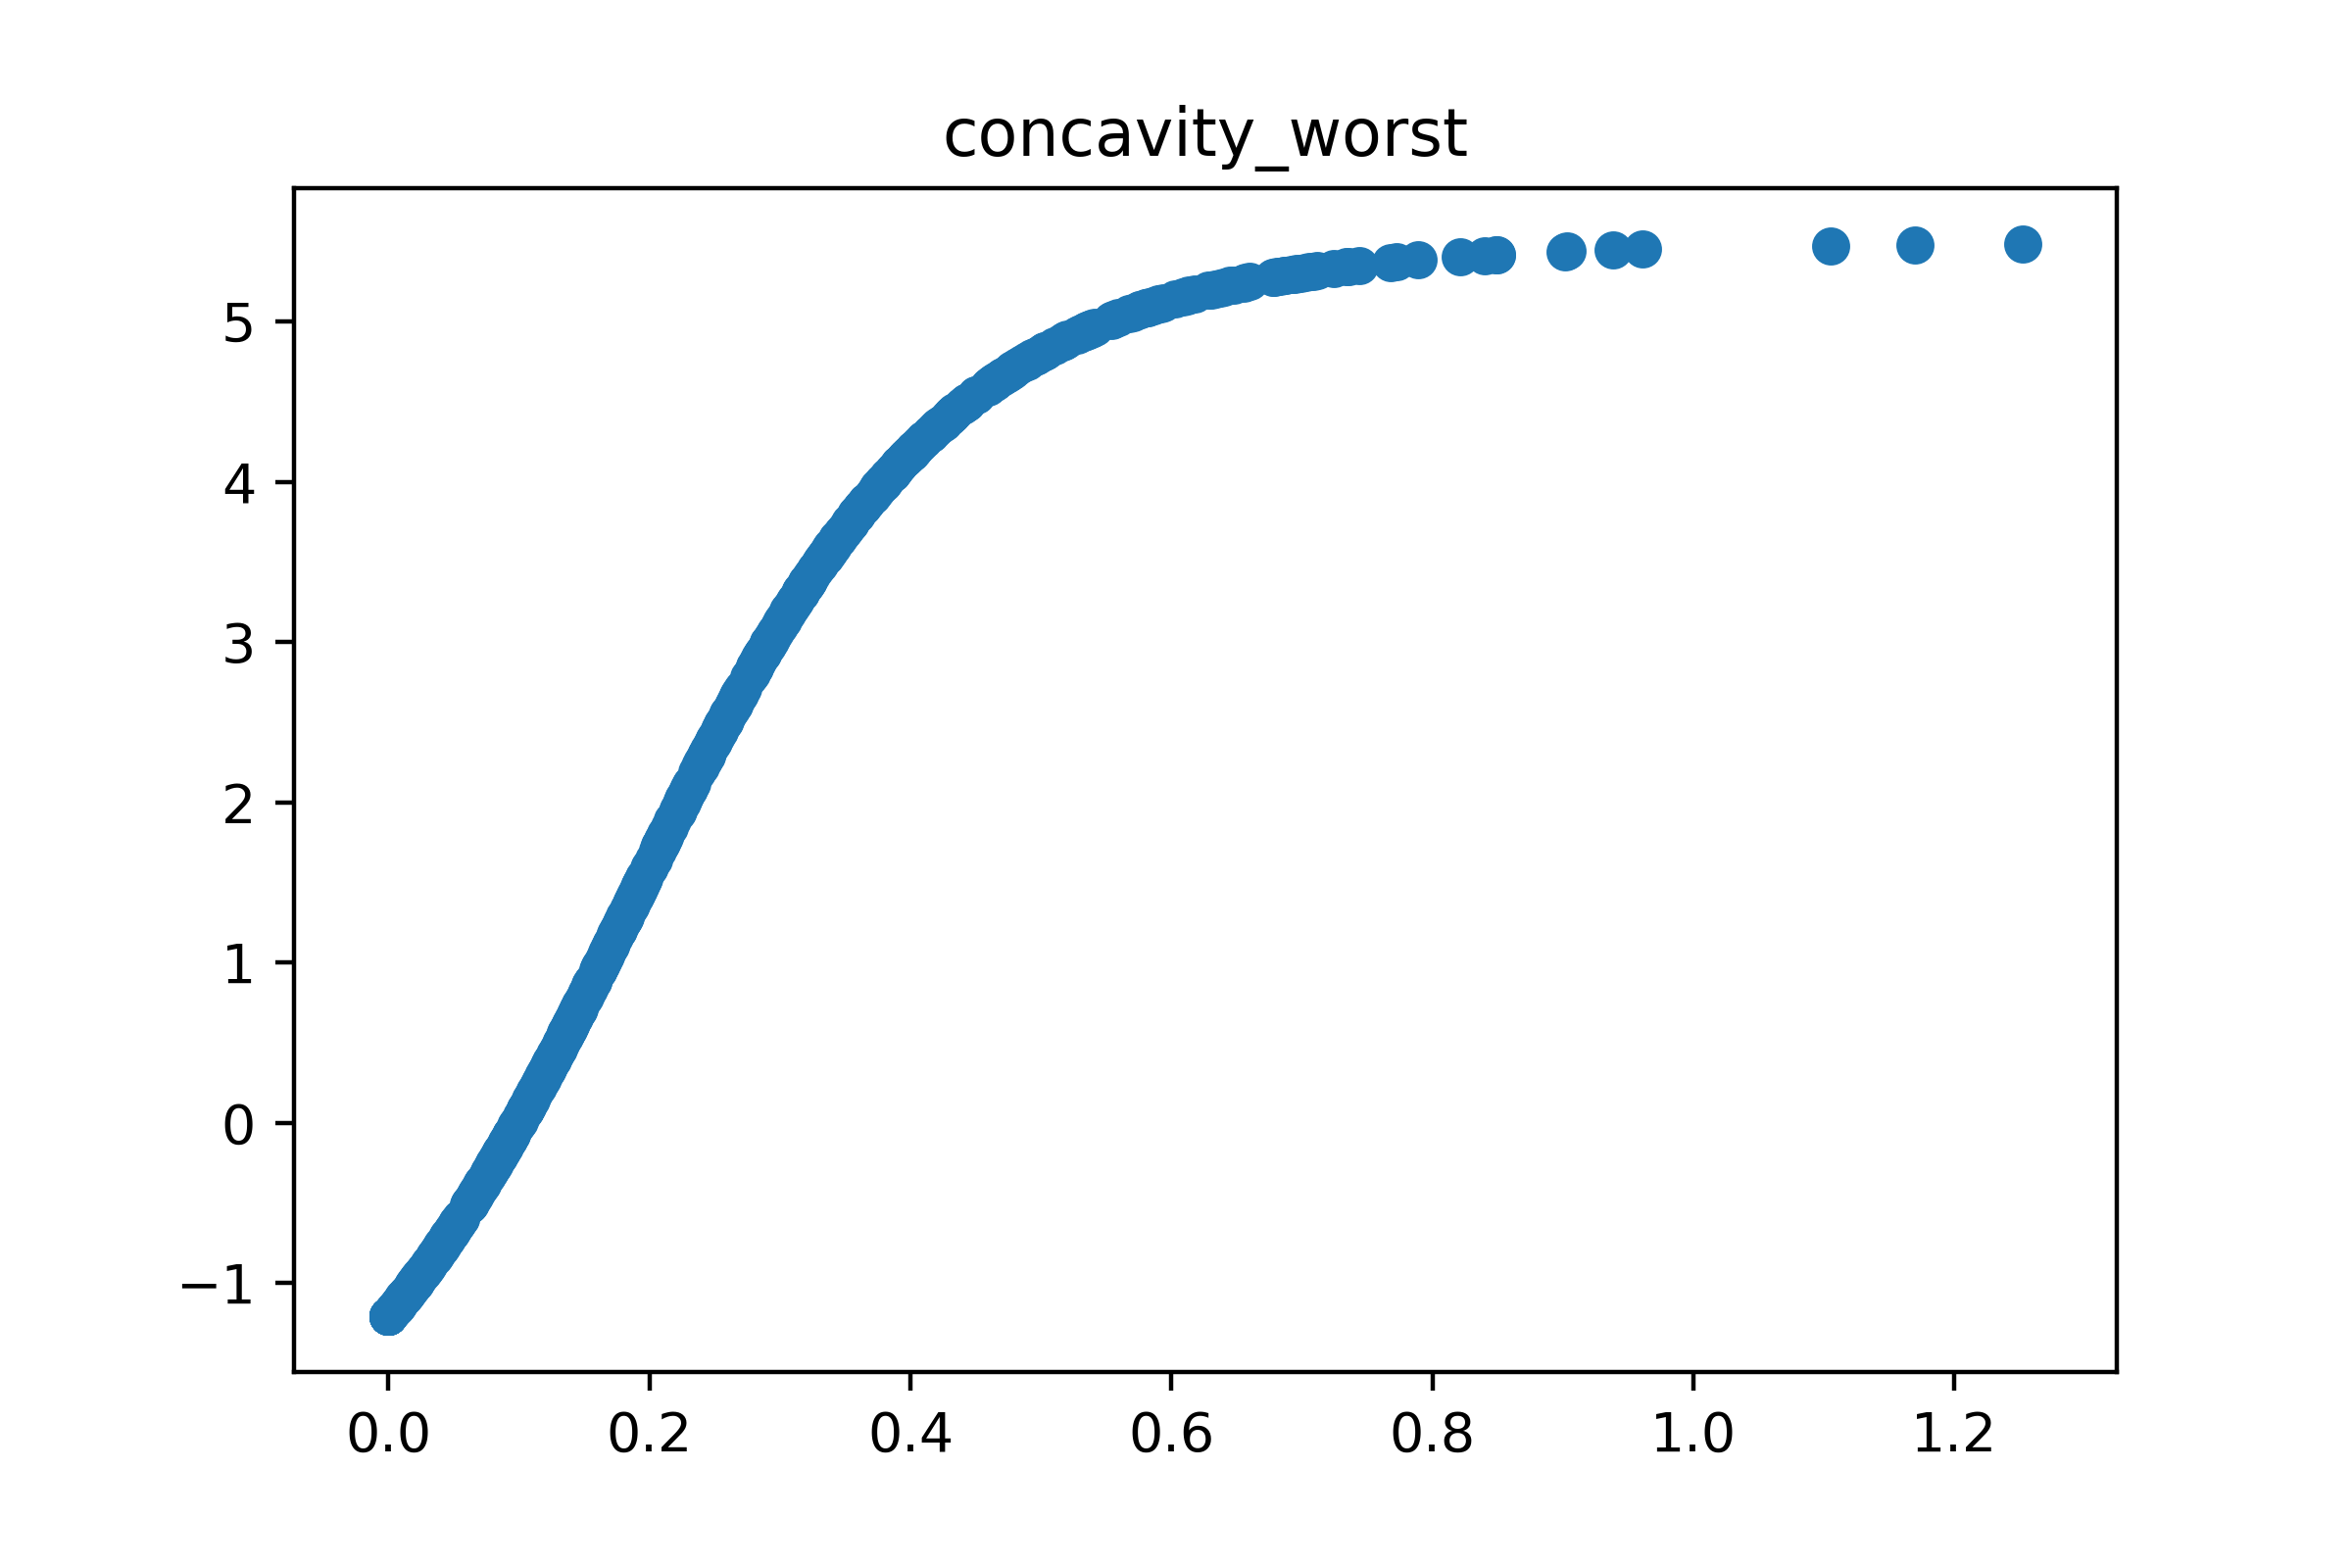
\includegraphics[width=0.40\textwidth]{fig/mnl/bc1.png} &
%     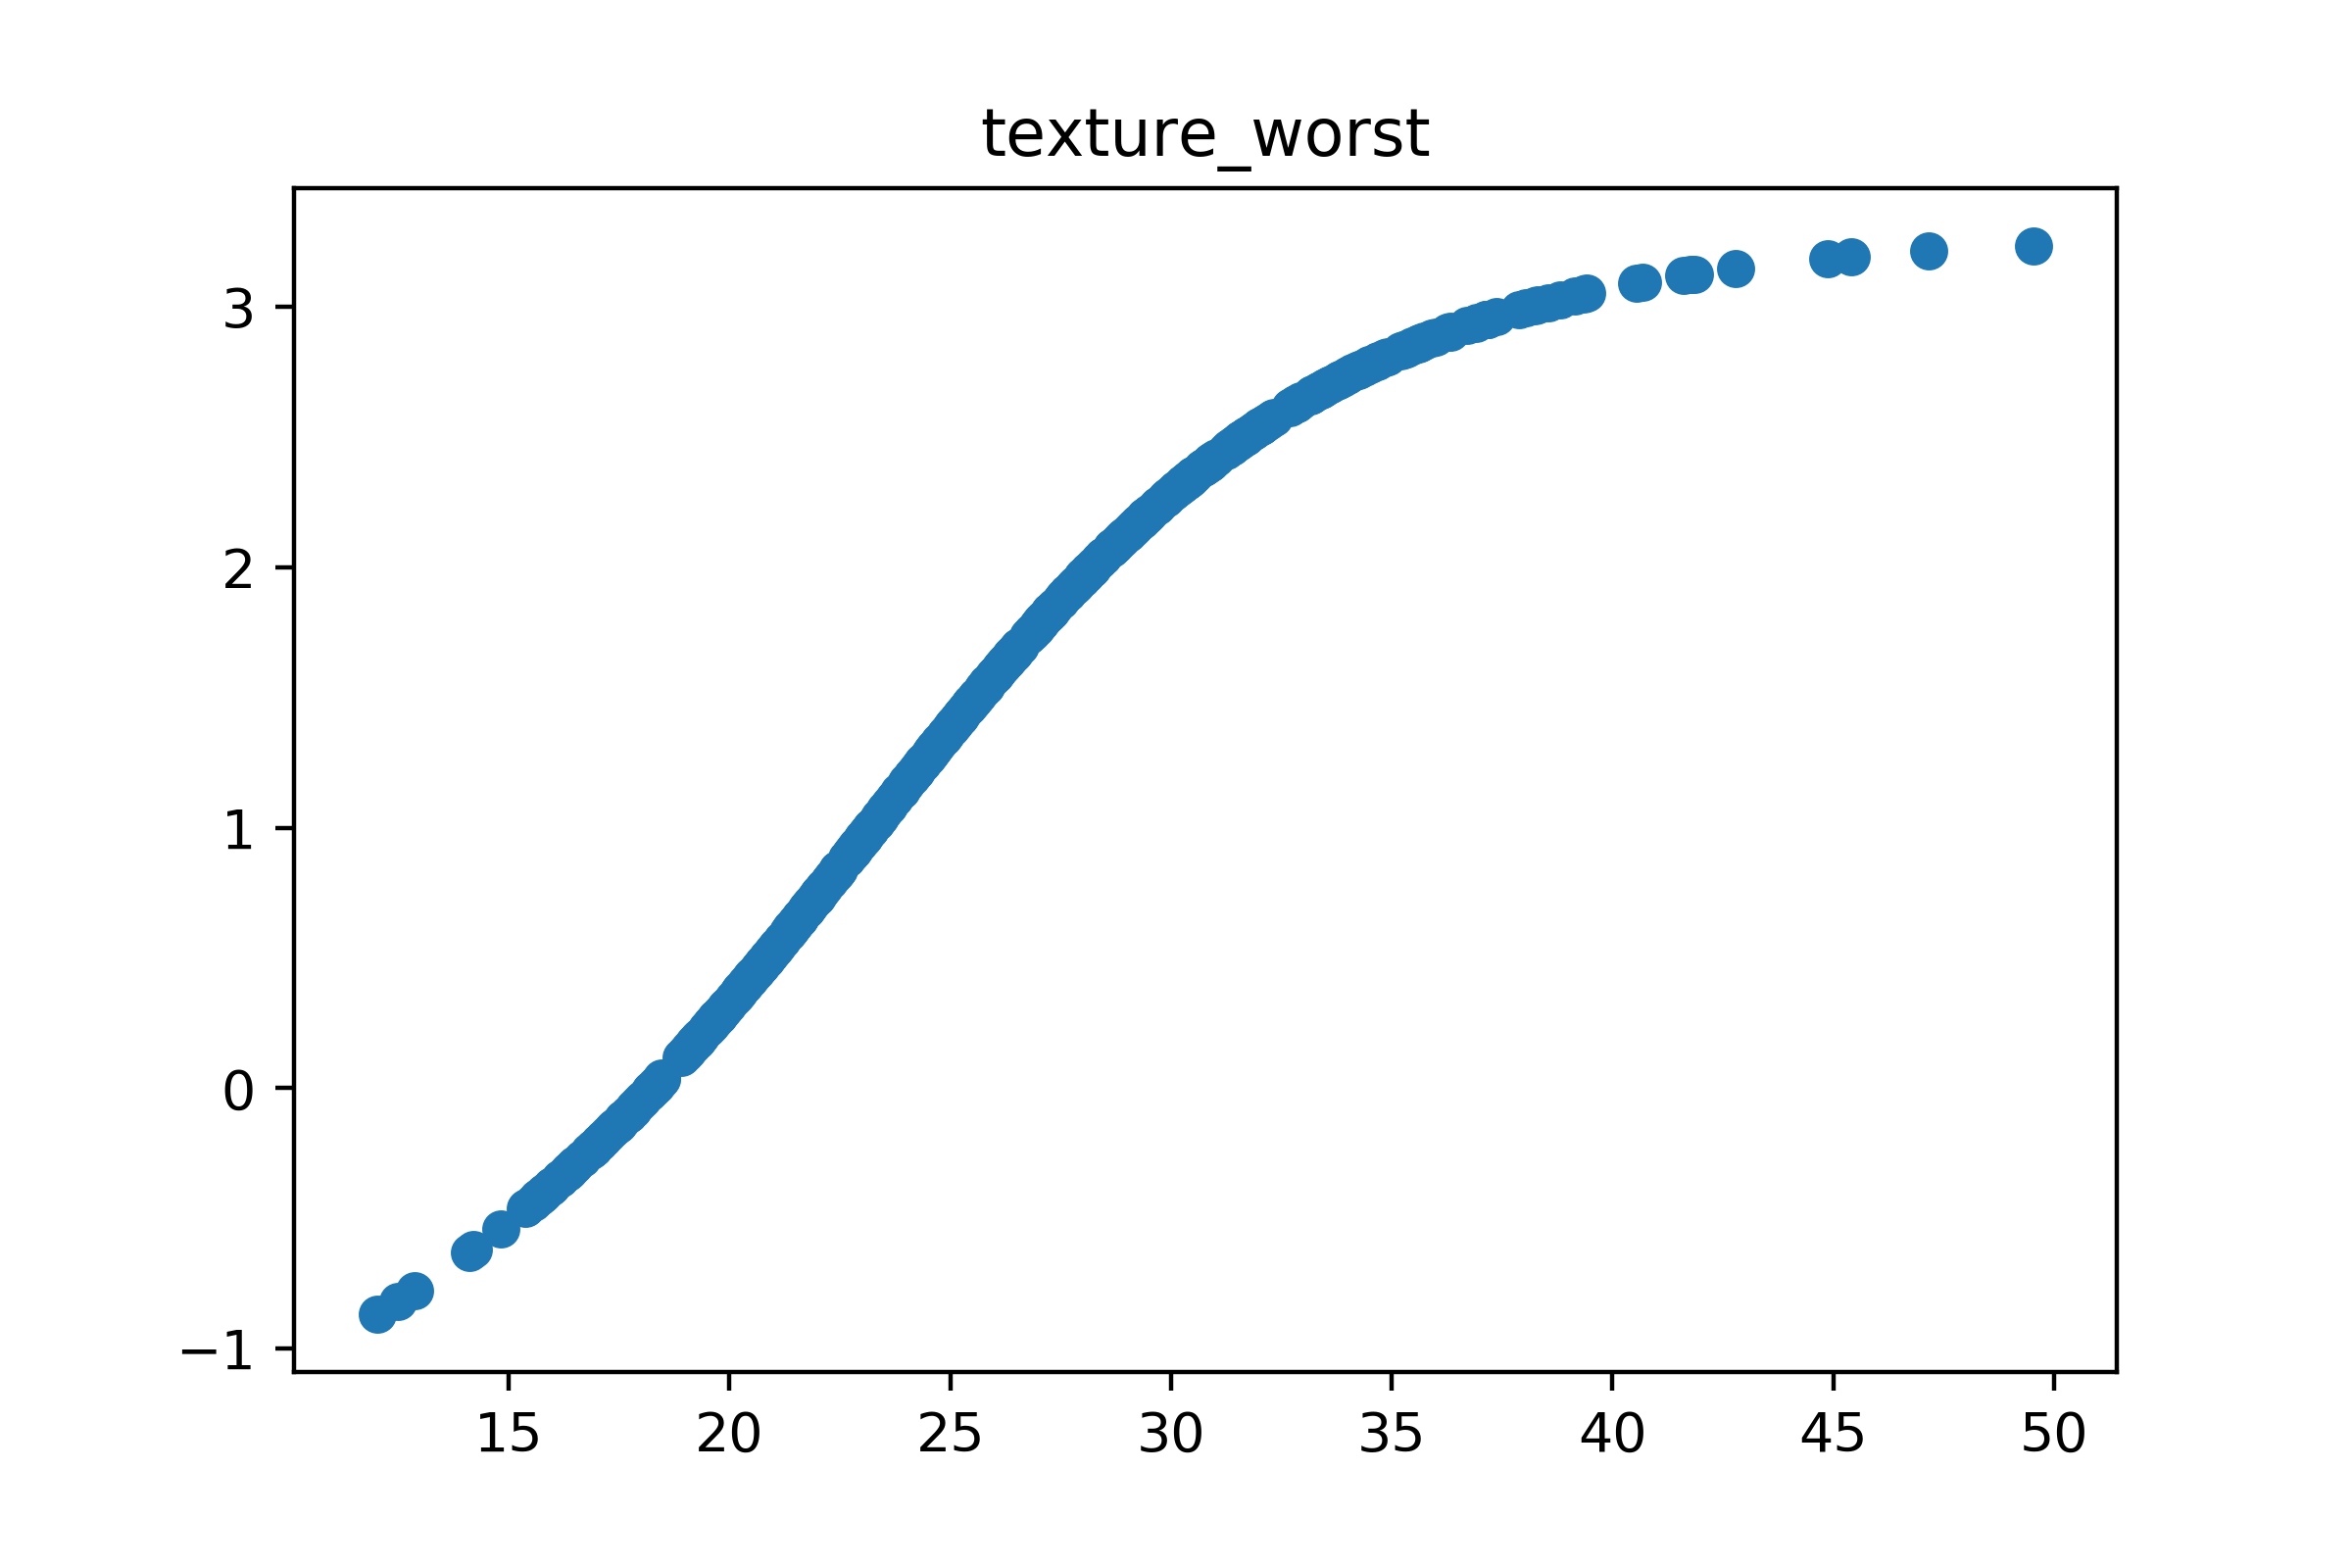
\includegraphics[width=0.40\textwidth]{fig/mnl/bc2.png}\tabularnewline
    
%     Sloan Sky Survey & 
%     %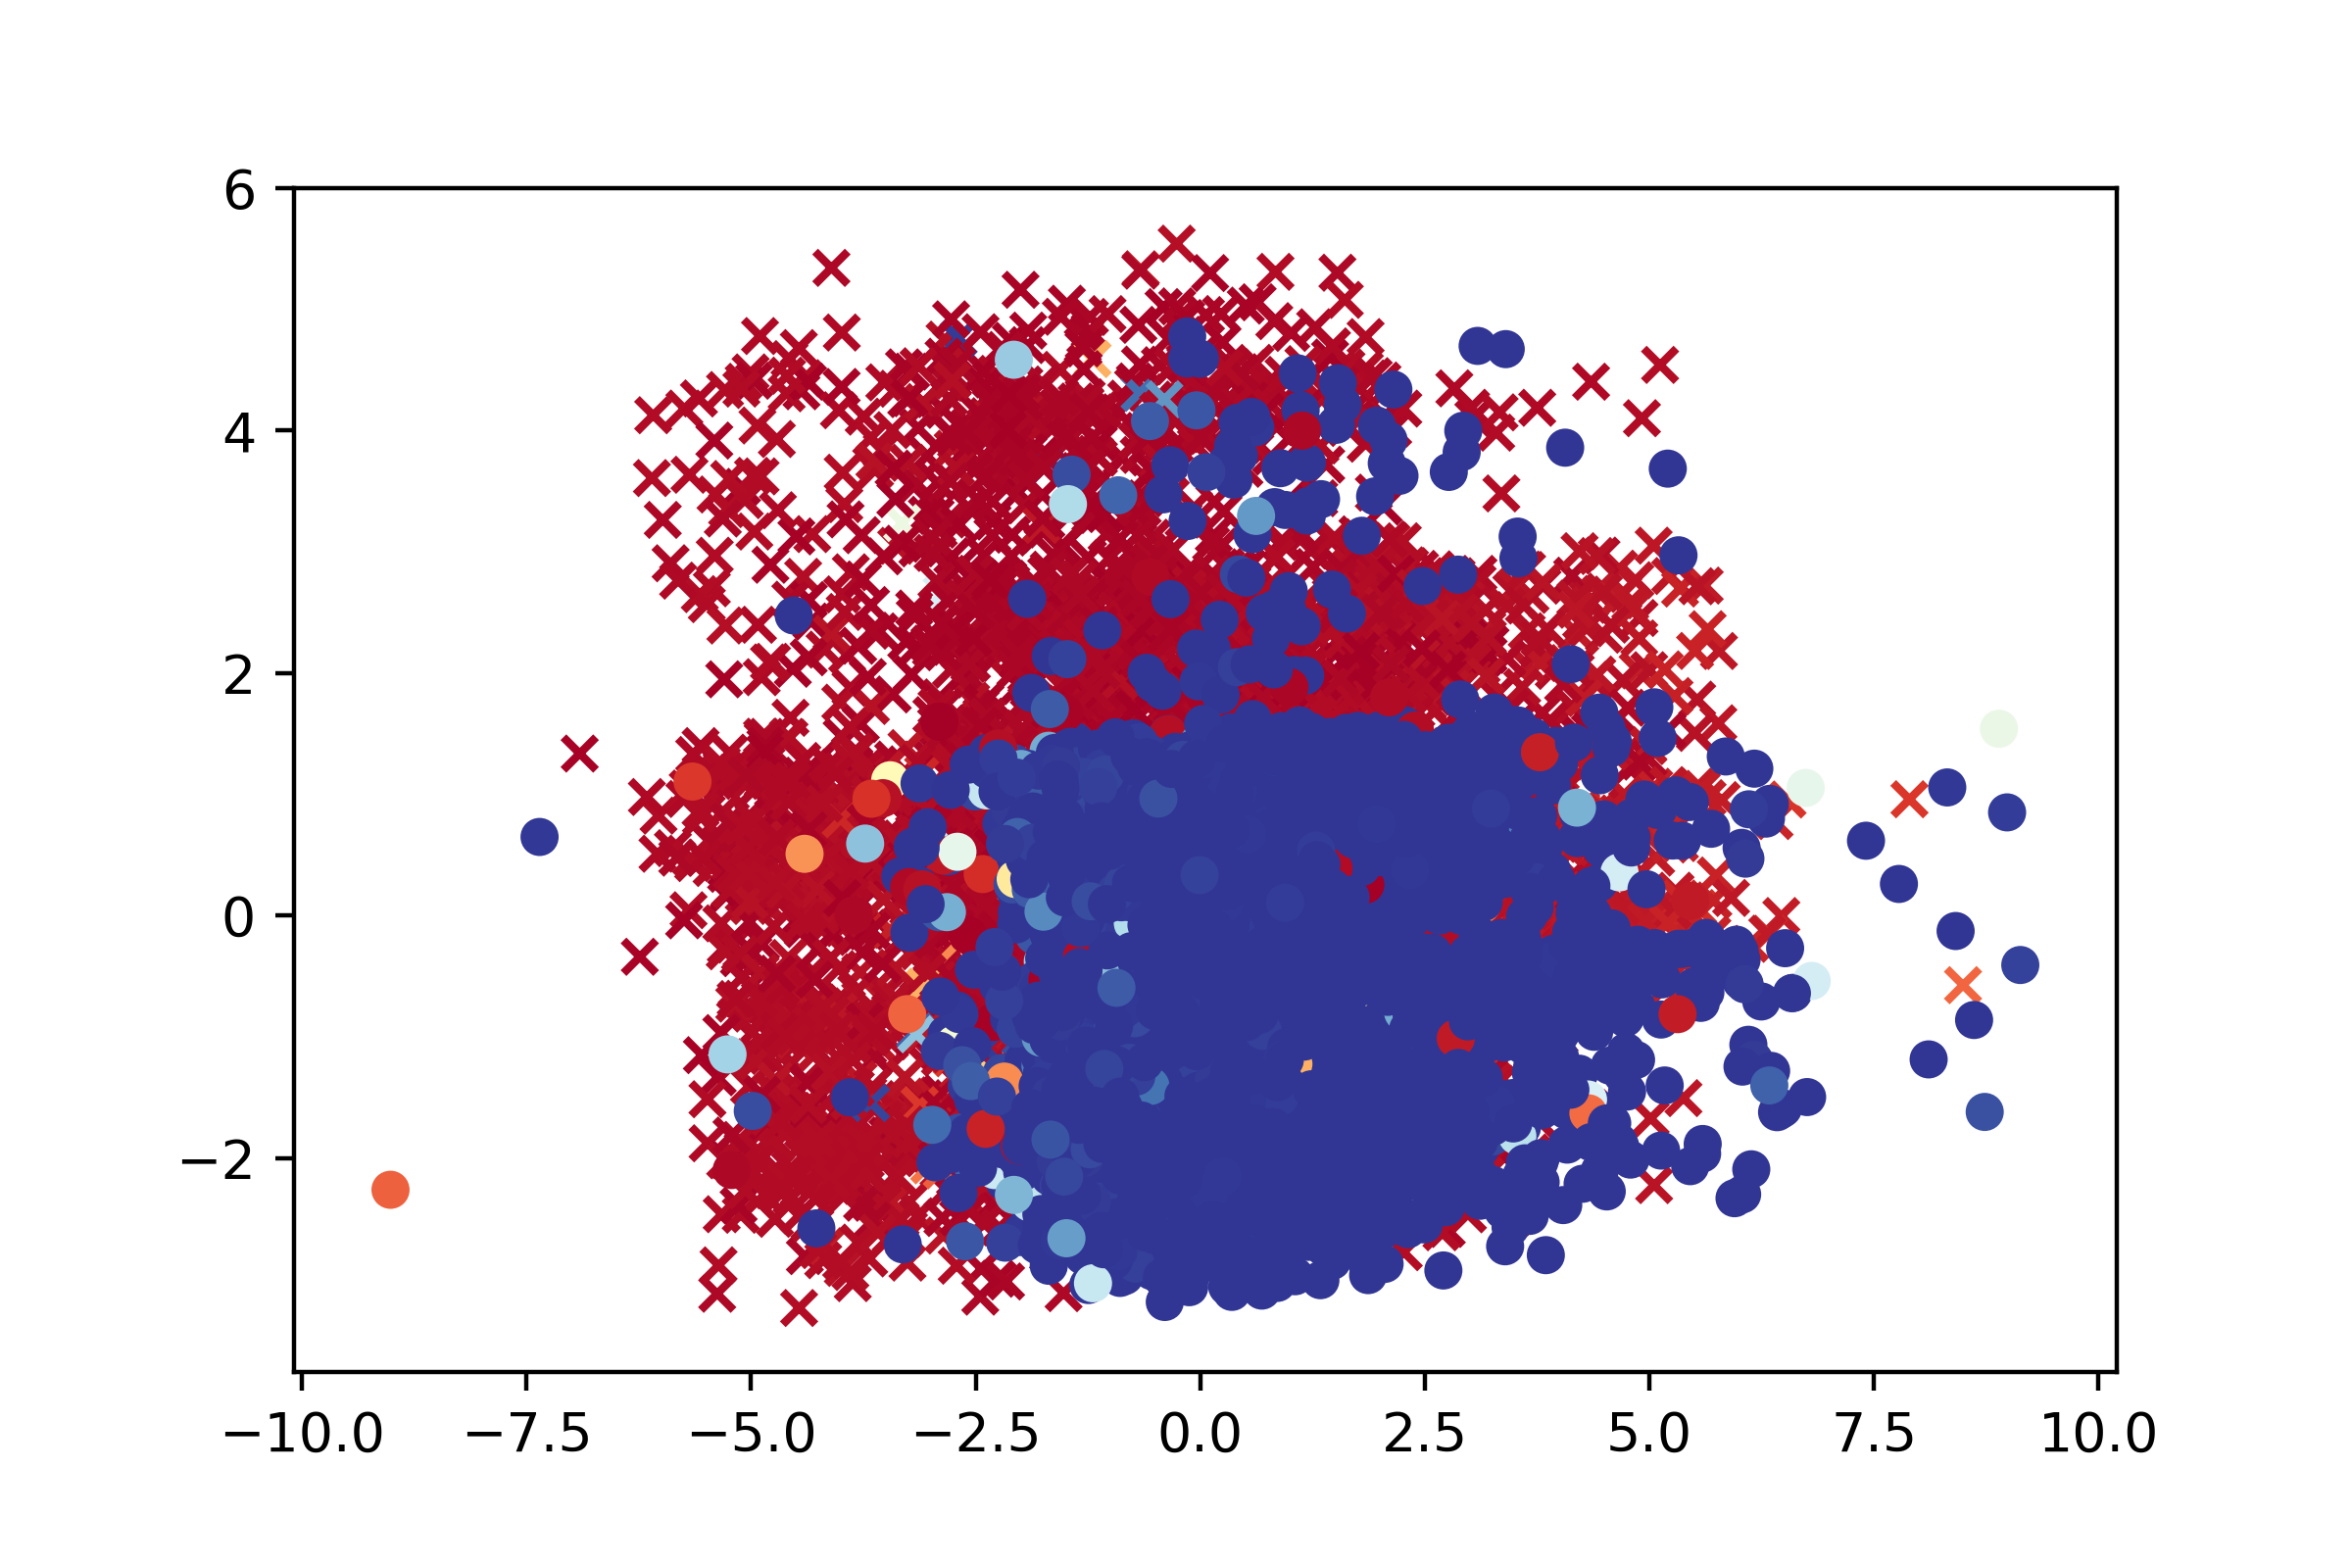
\includegraphics[width=0.22\textwidth]{fig/plt/st.png} &
%     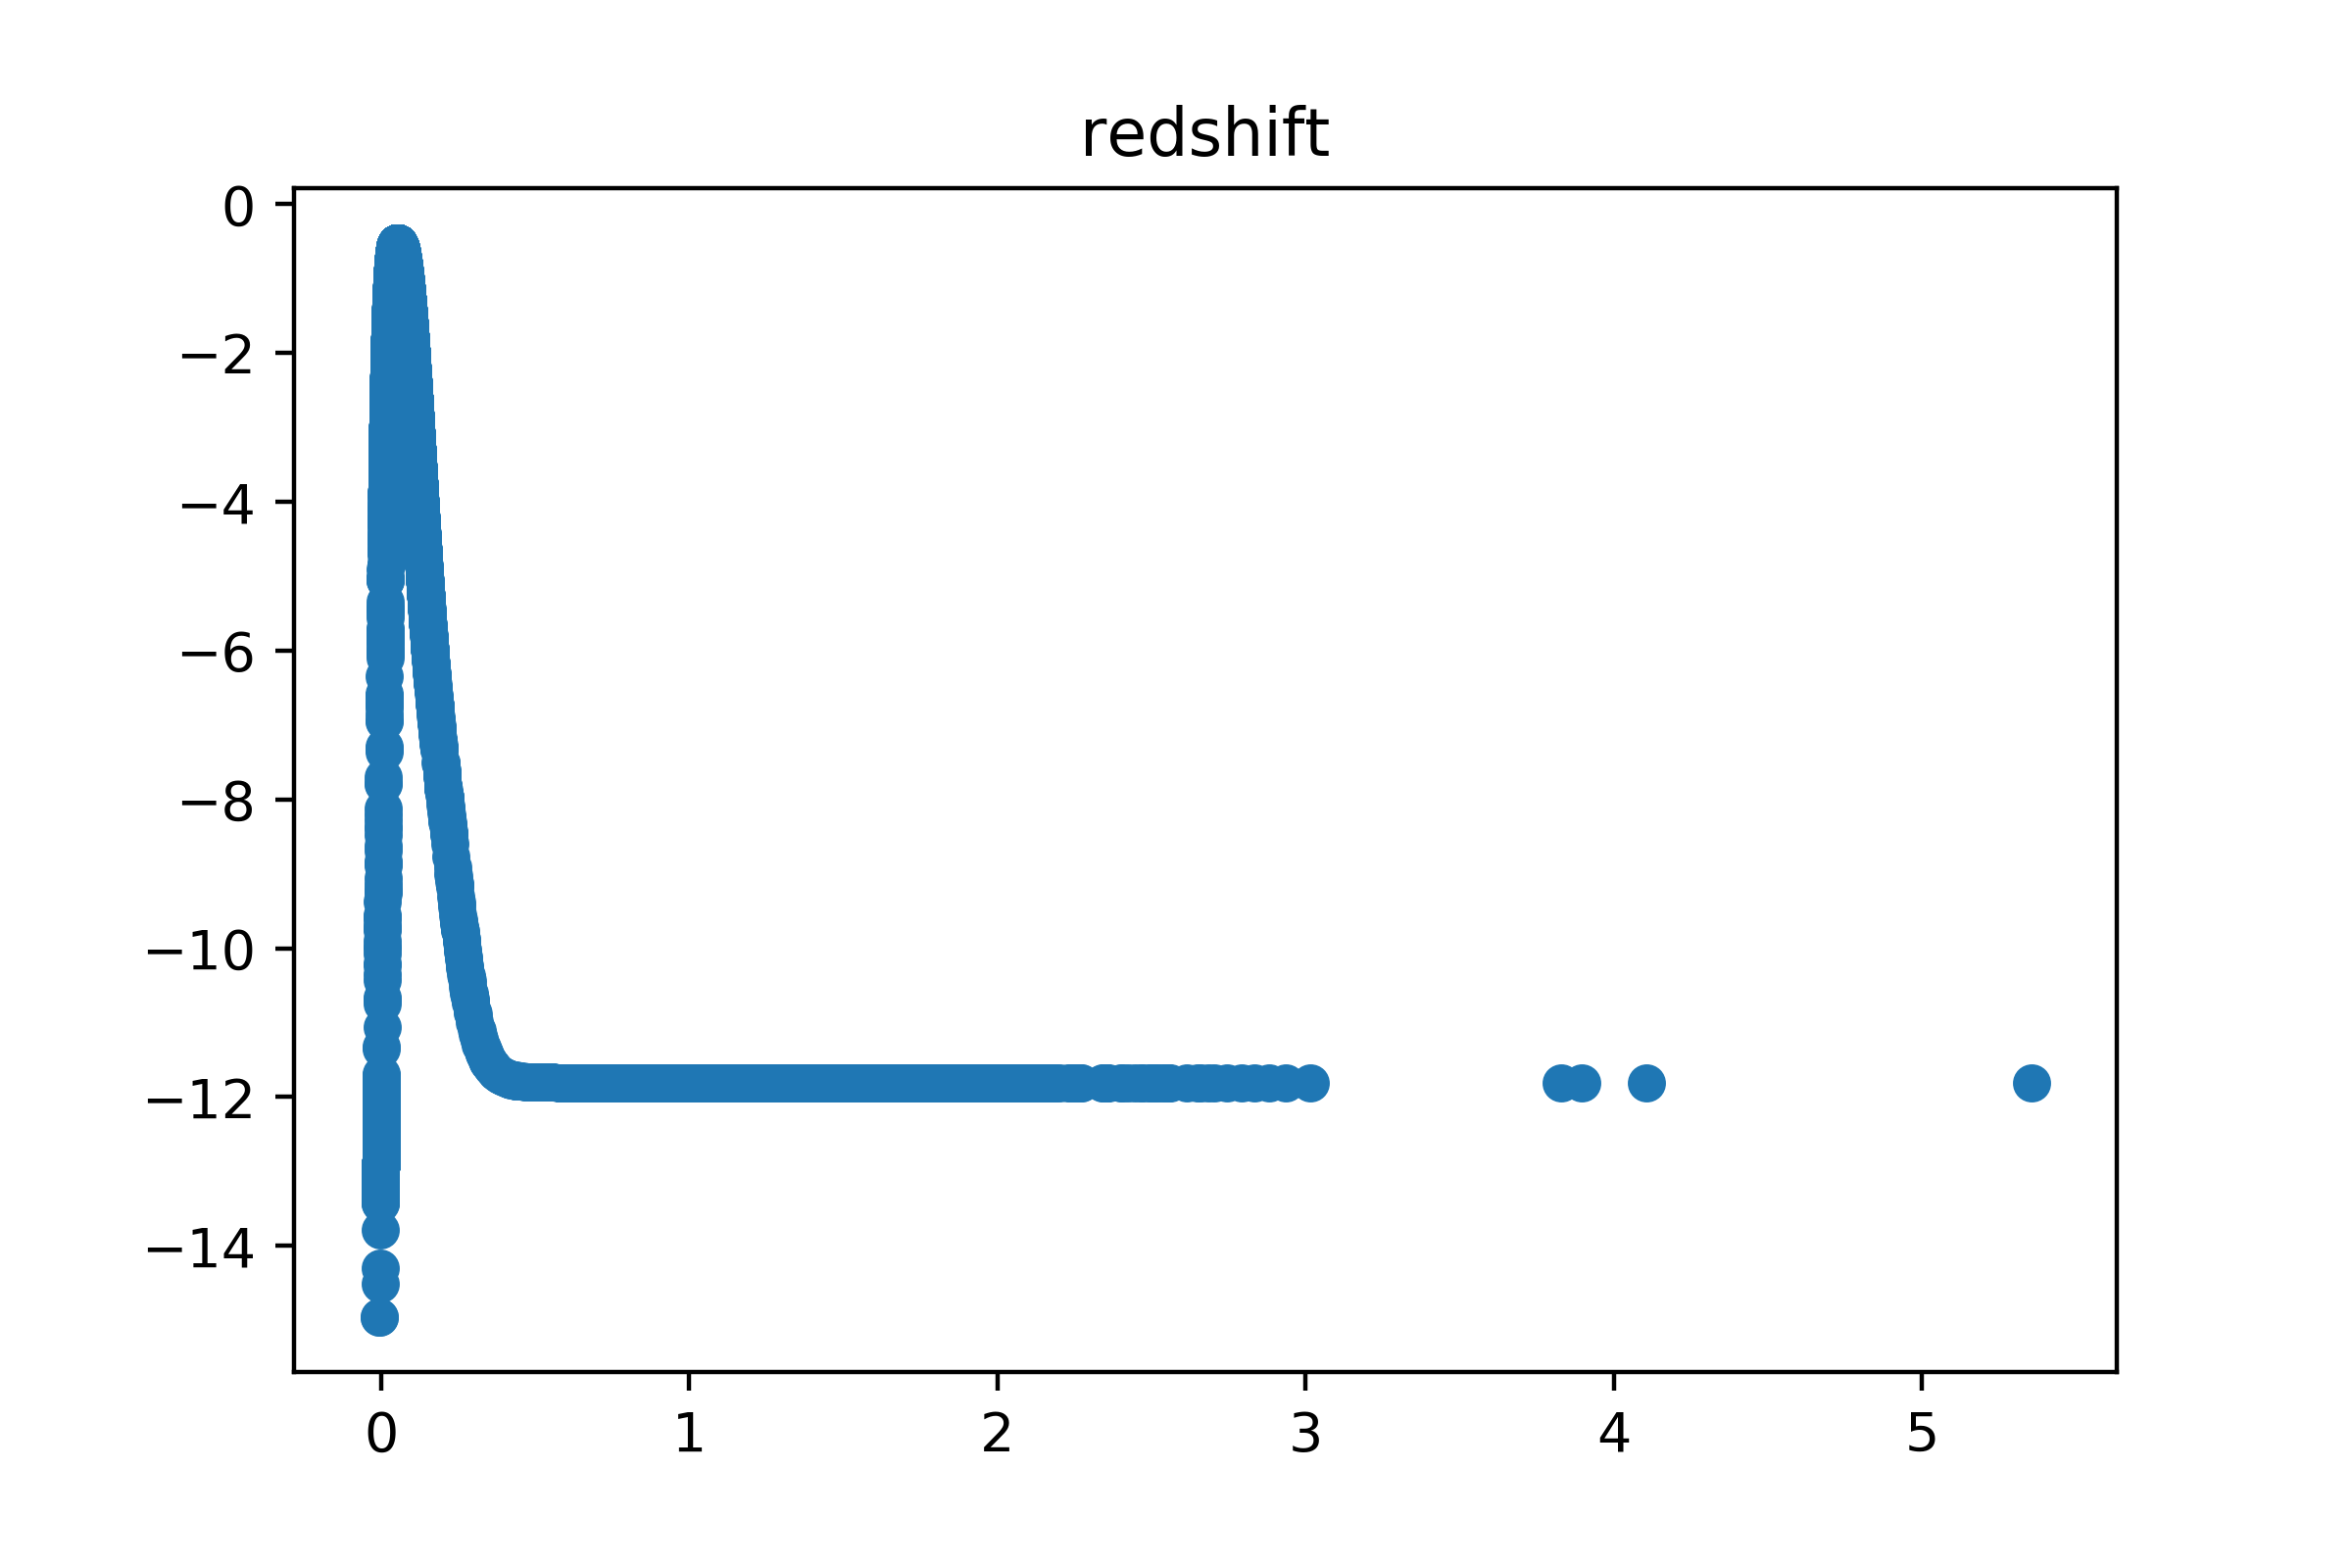
\includegraphics[width=0.40\textwidth]{fig/mnl/st1.png} &
%     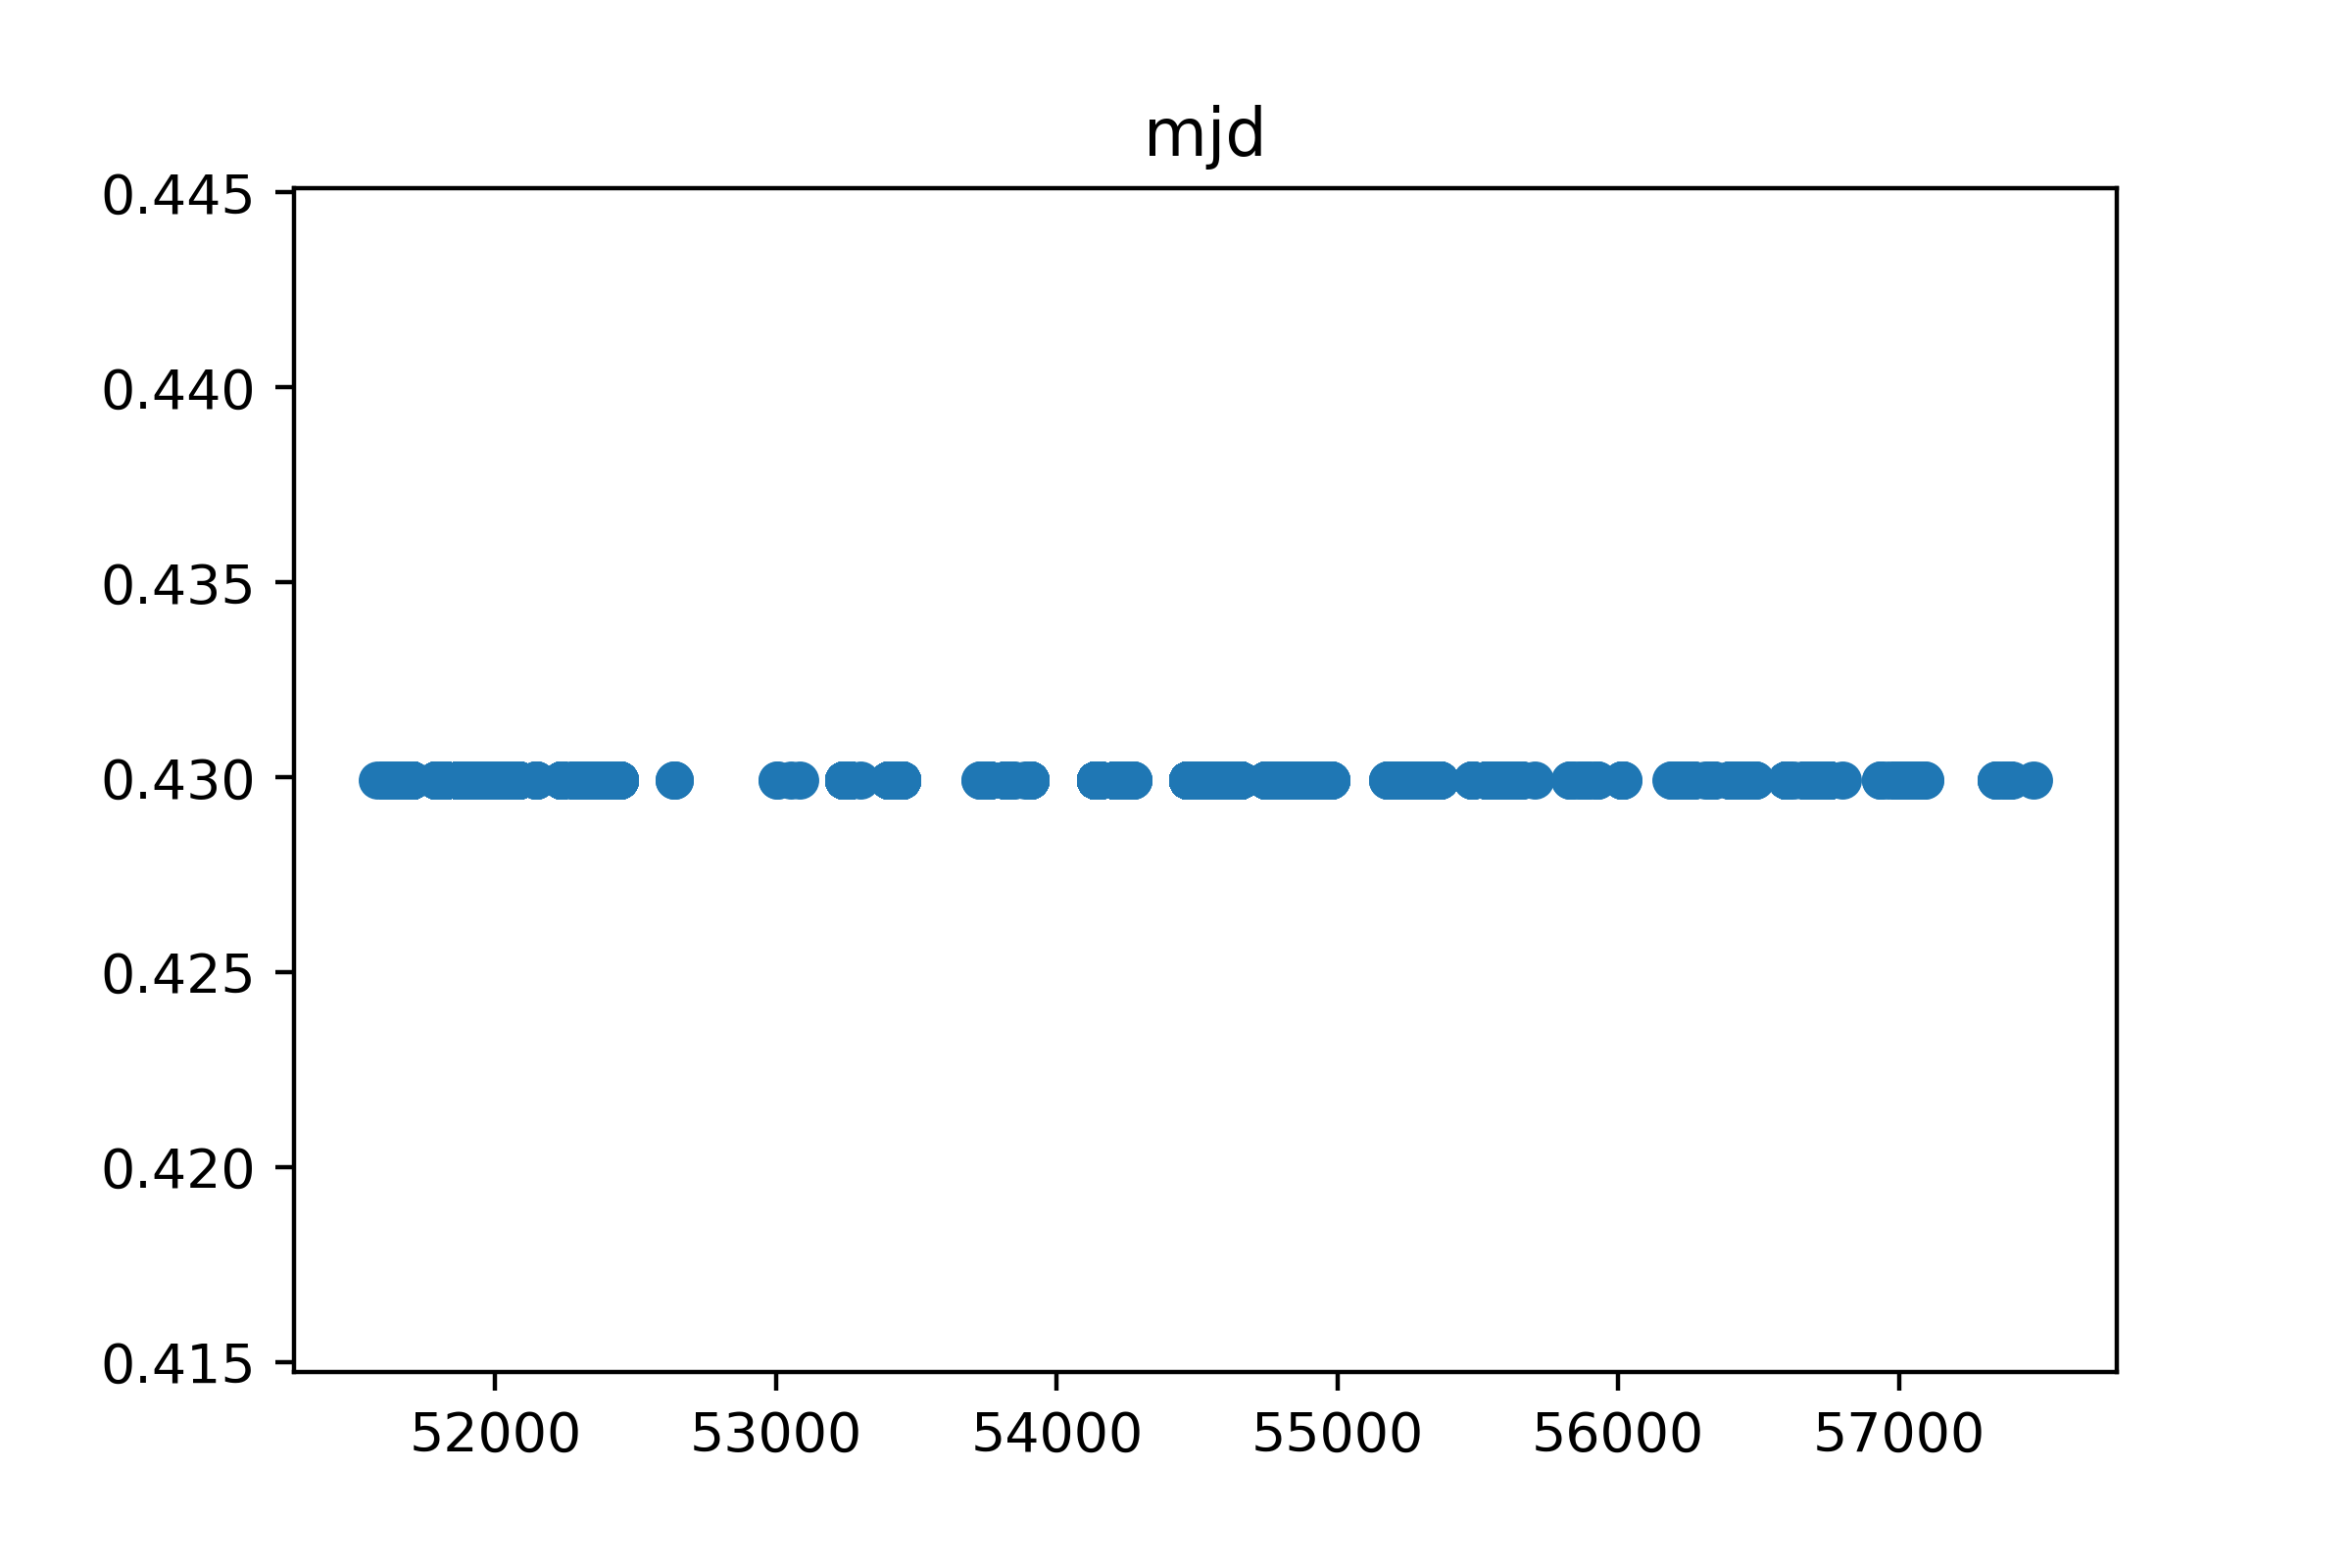
\includegraphics[width=0.40\textwidth]{fig/mnl/st2.png}\tabularnewline
    
%     Iris & 
%     %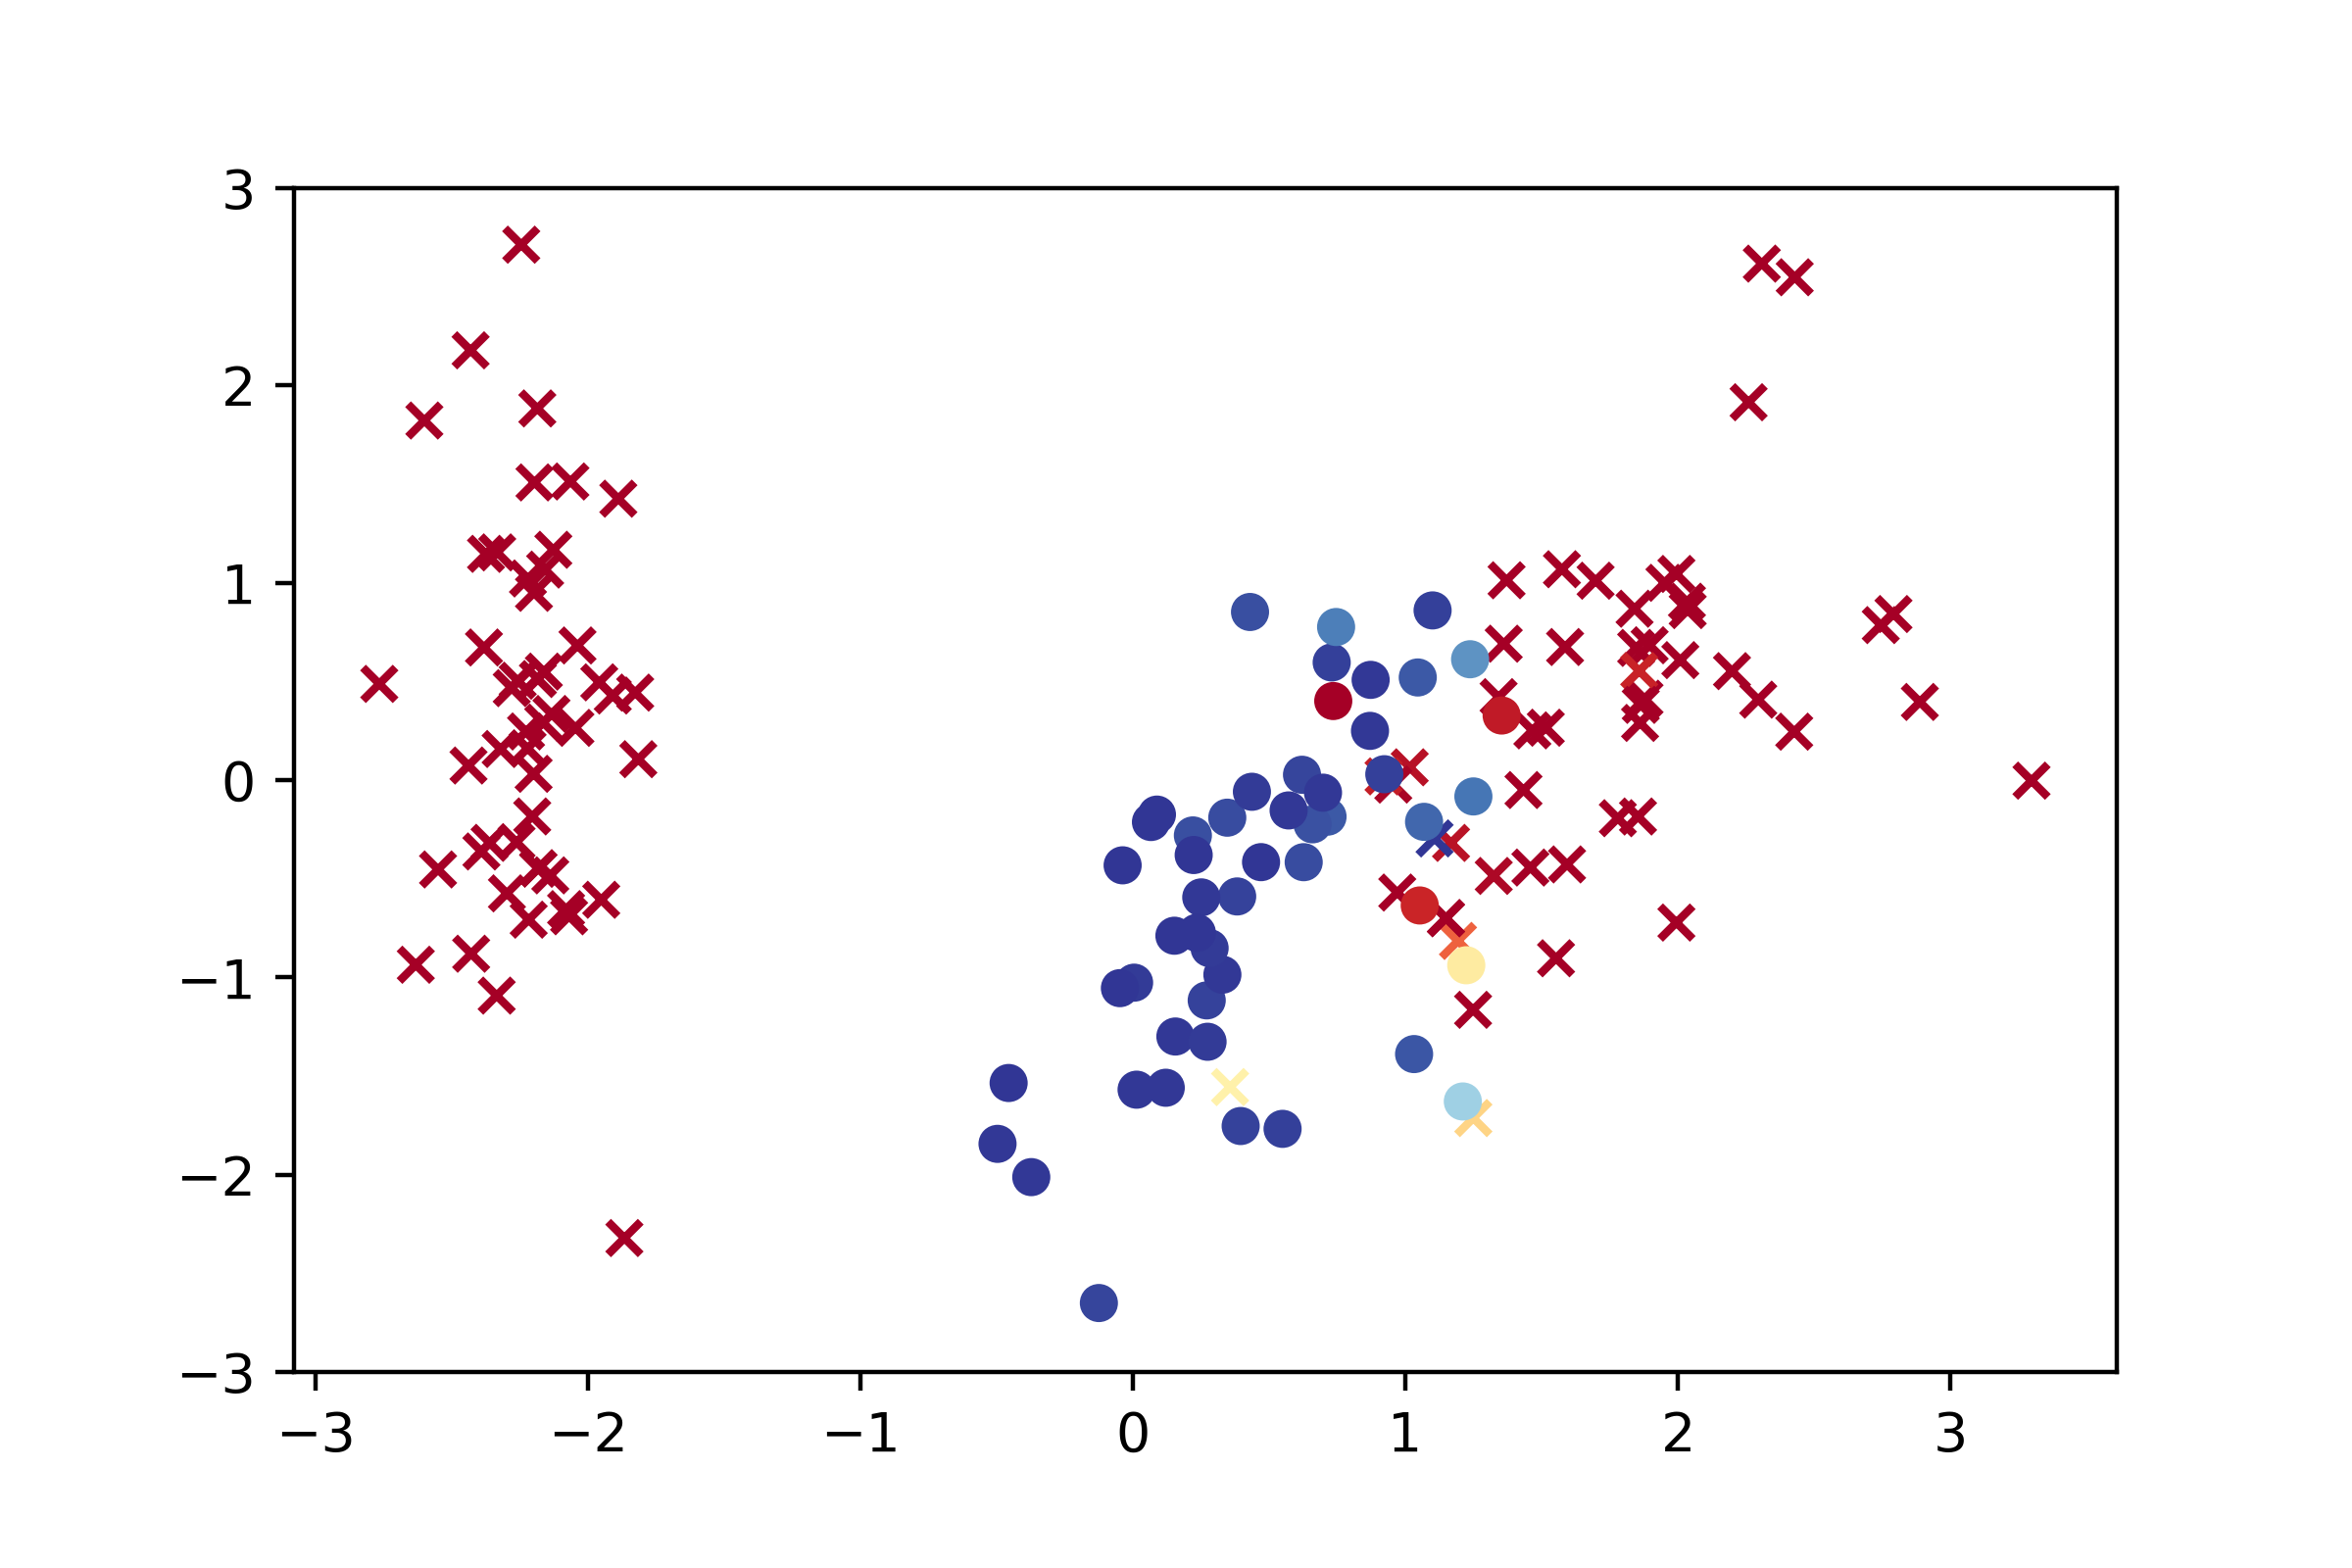
\includegraphics[width=0.22\textwidth]{fig/plt/ir.png} &
%     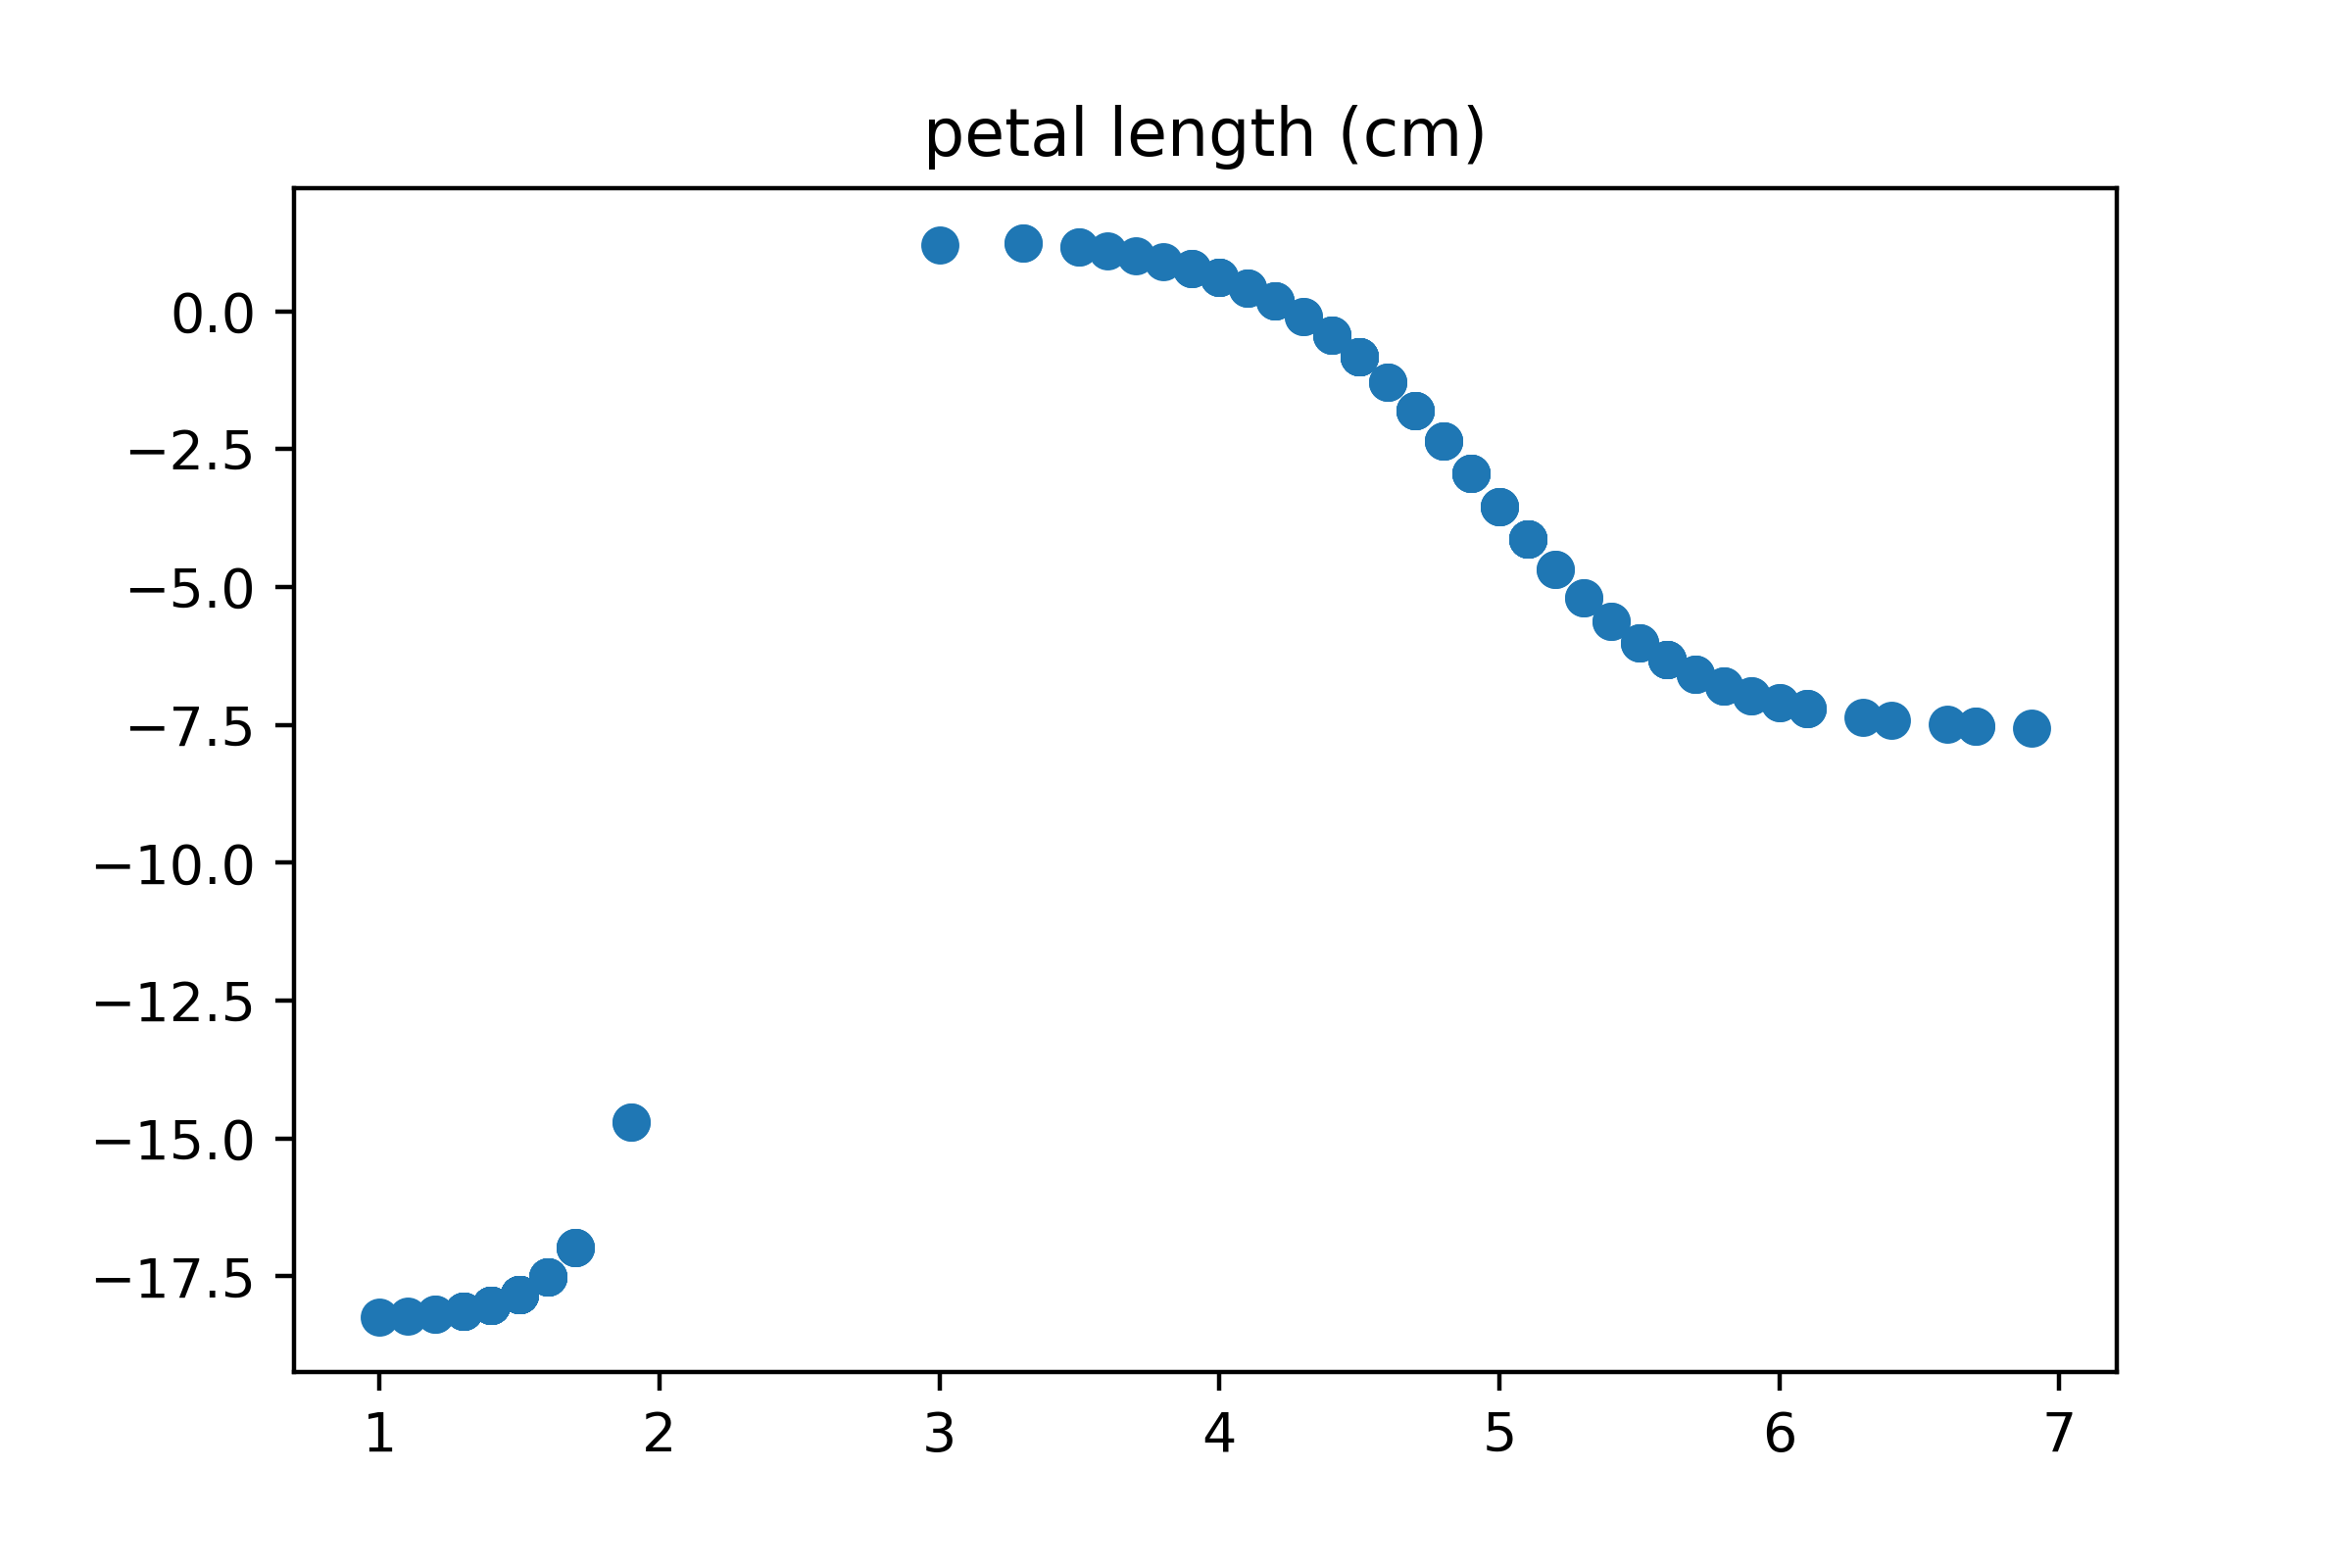
\includegraphics[width=0.40\textwidth]{fig/mnl/ir1.png} &
%     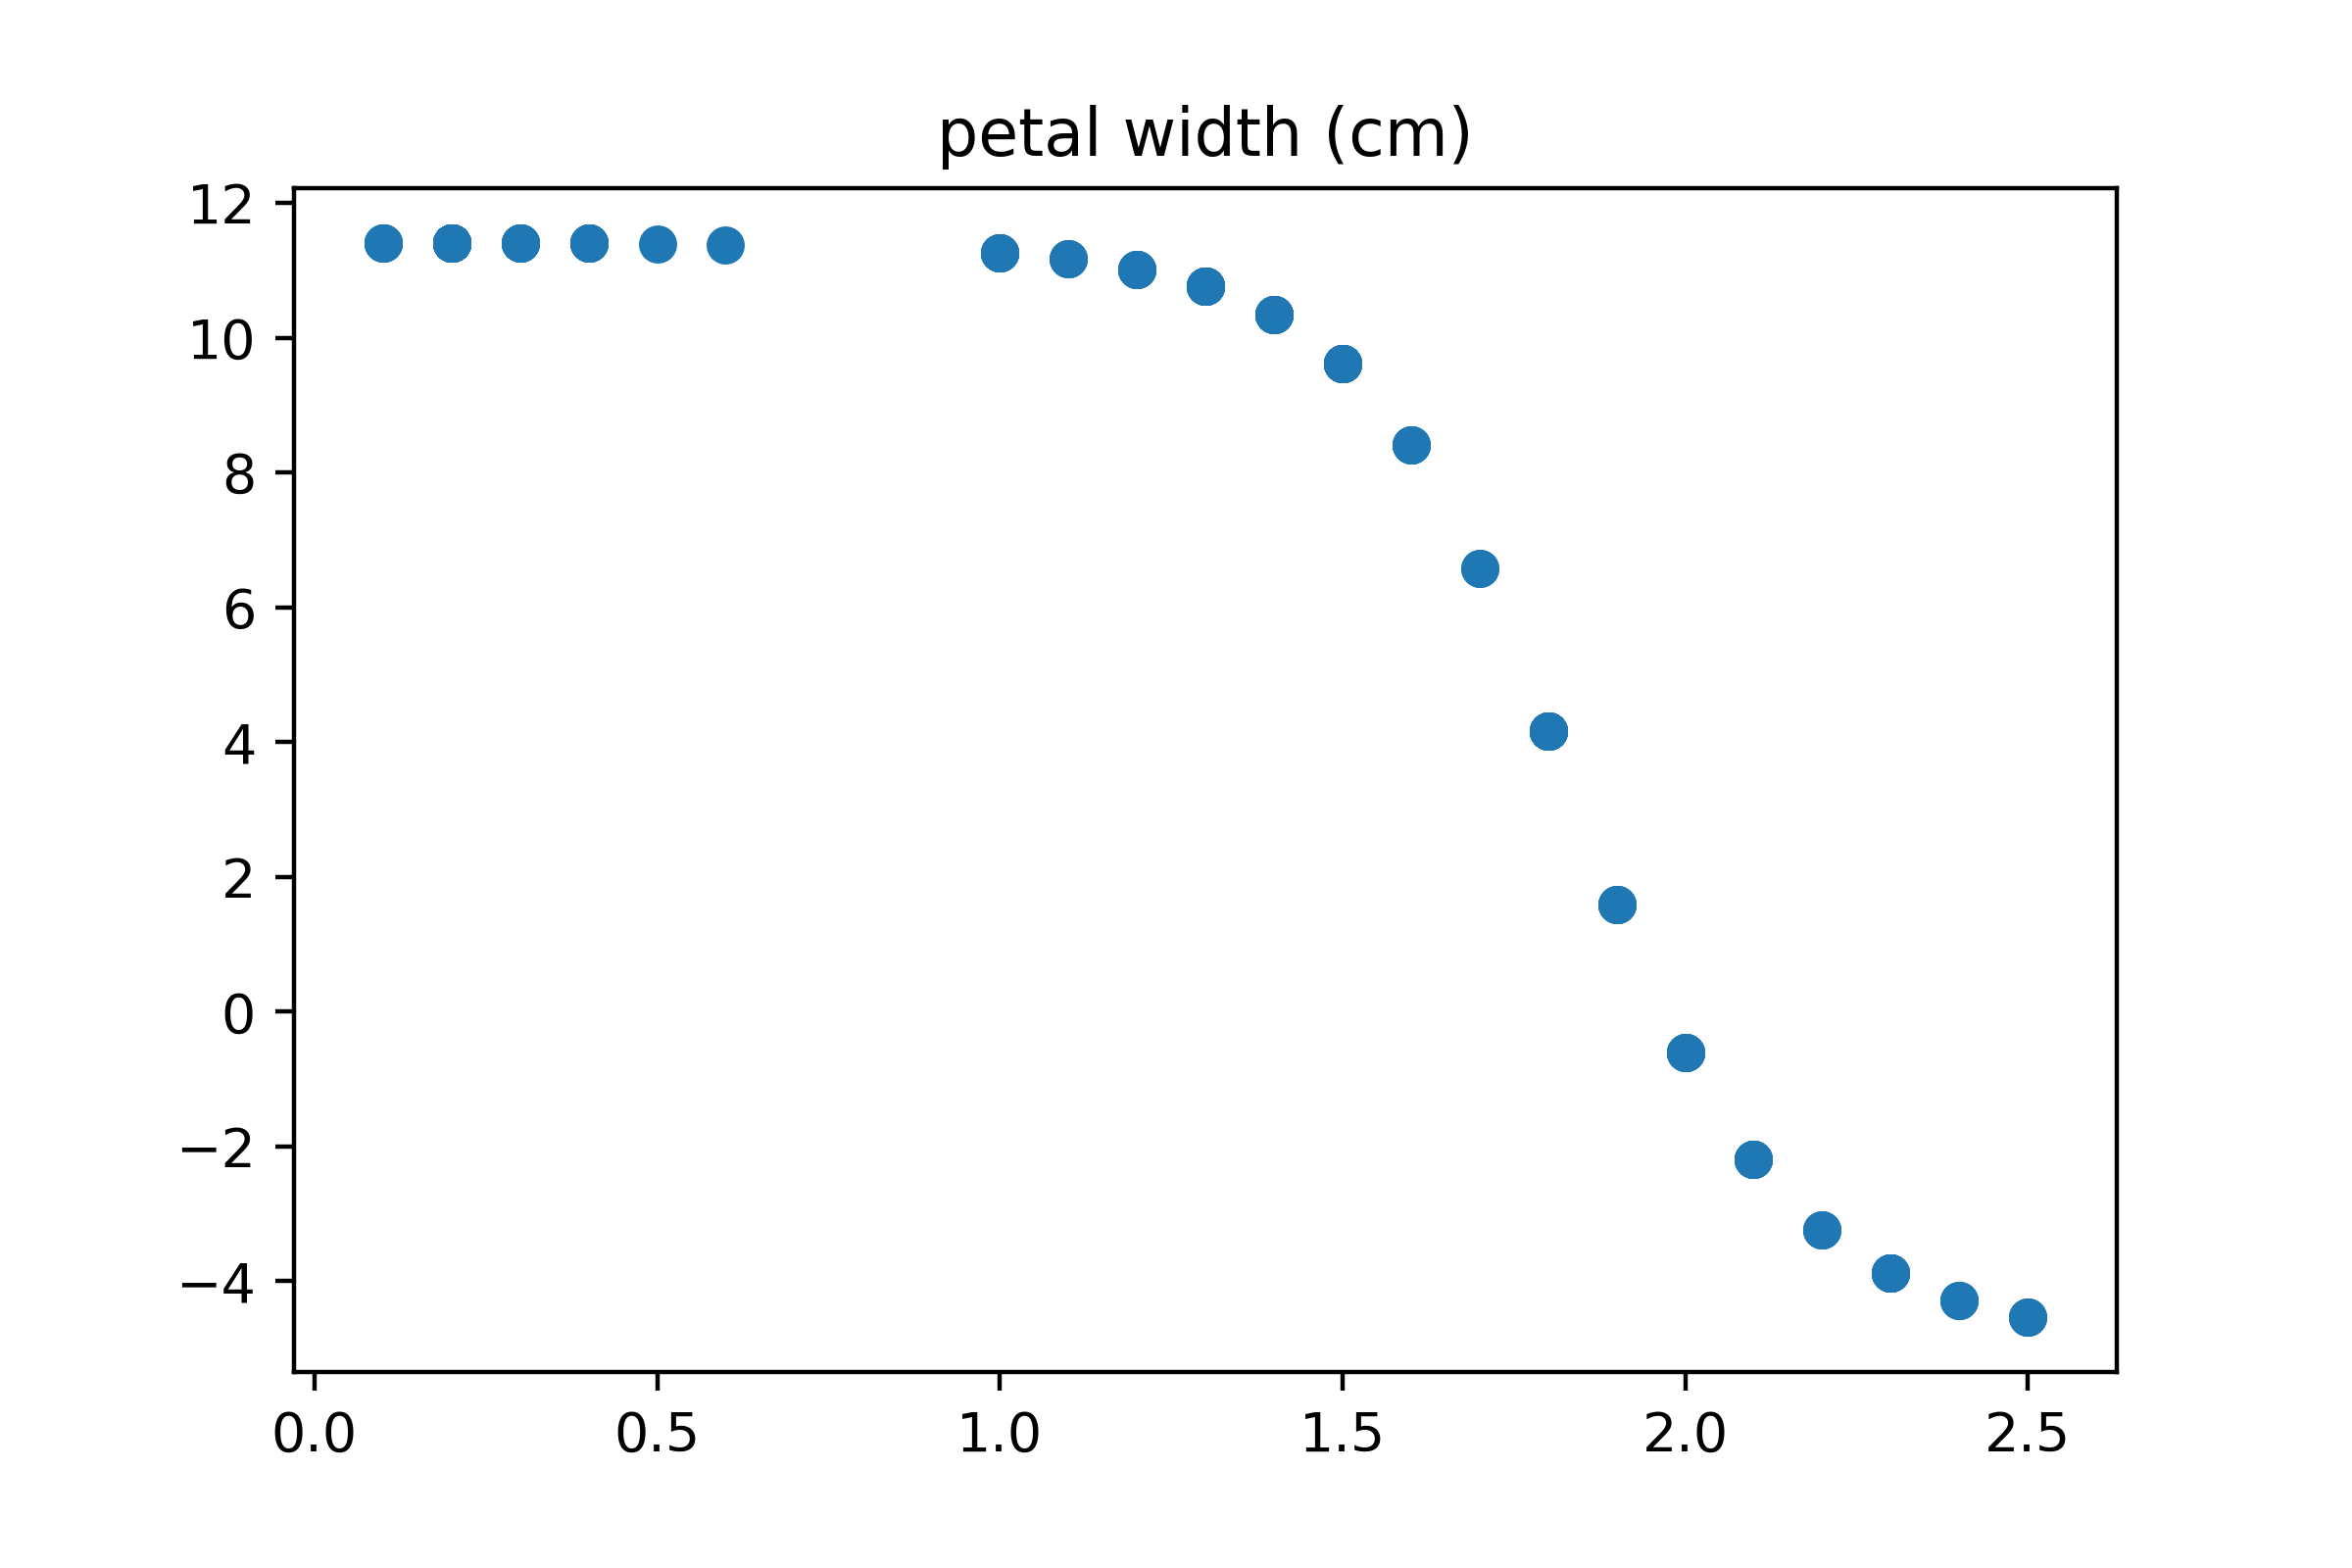
\includegraphics[width=0.40\textwidth]{fig/mnl/ir2.png}\tabularnewline
    
%     Titanic & 
%     %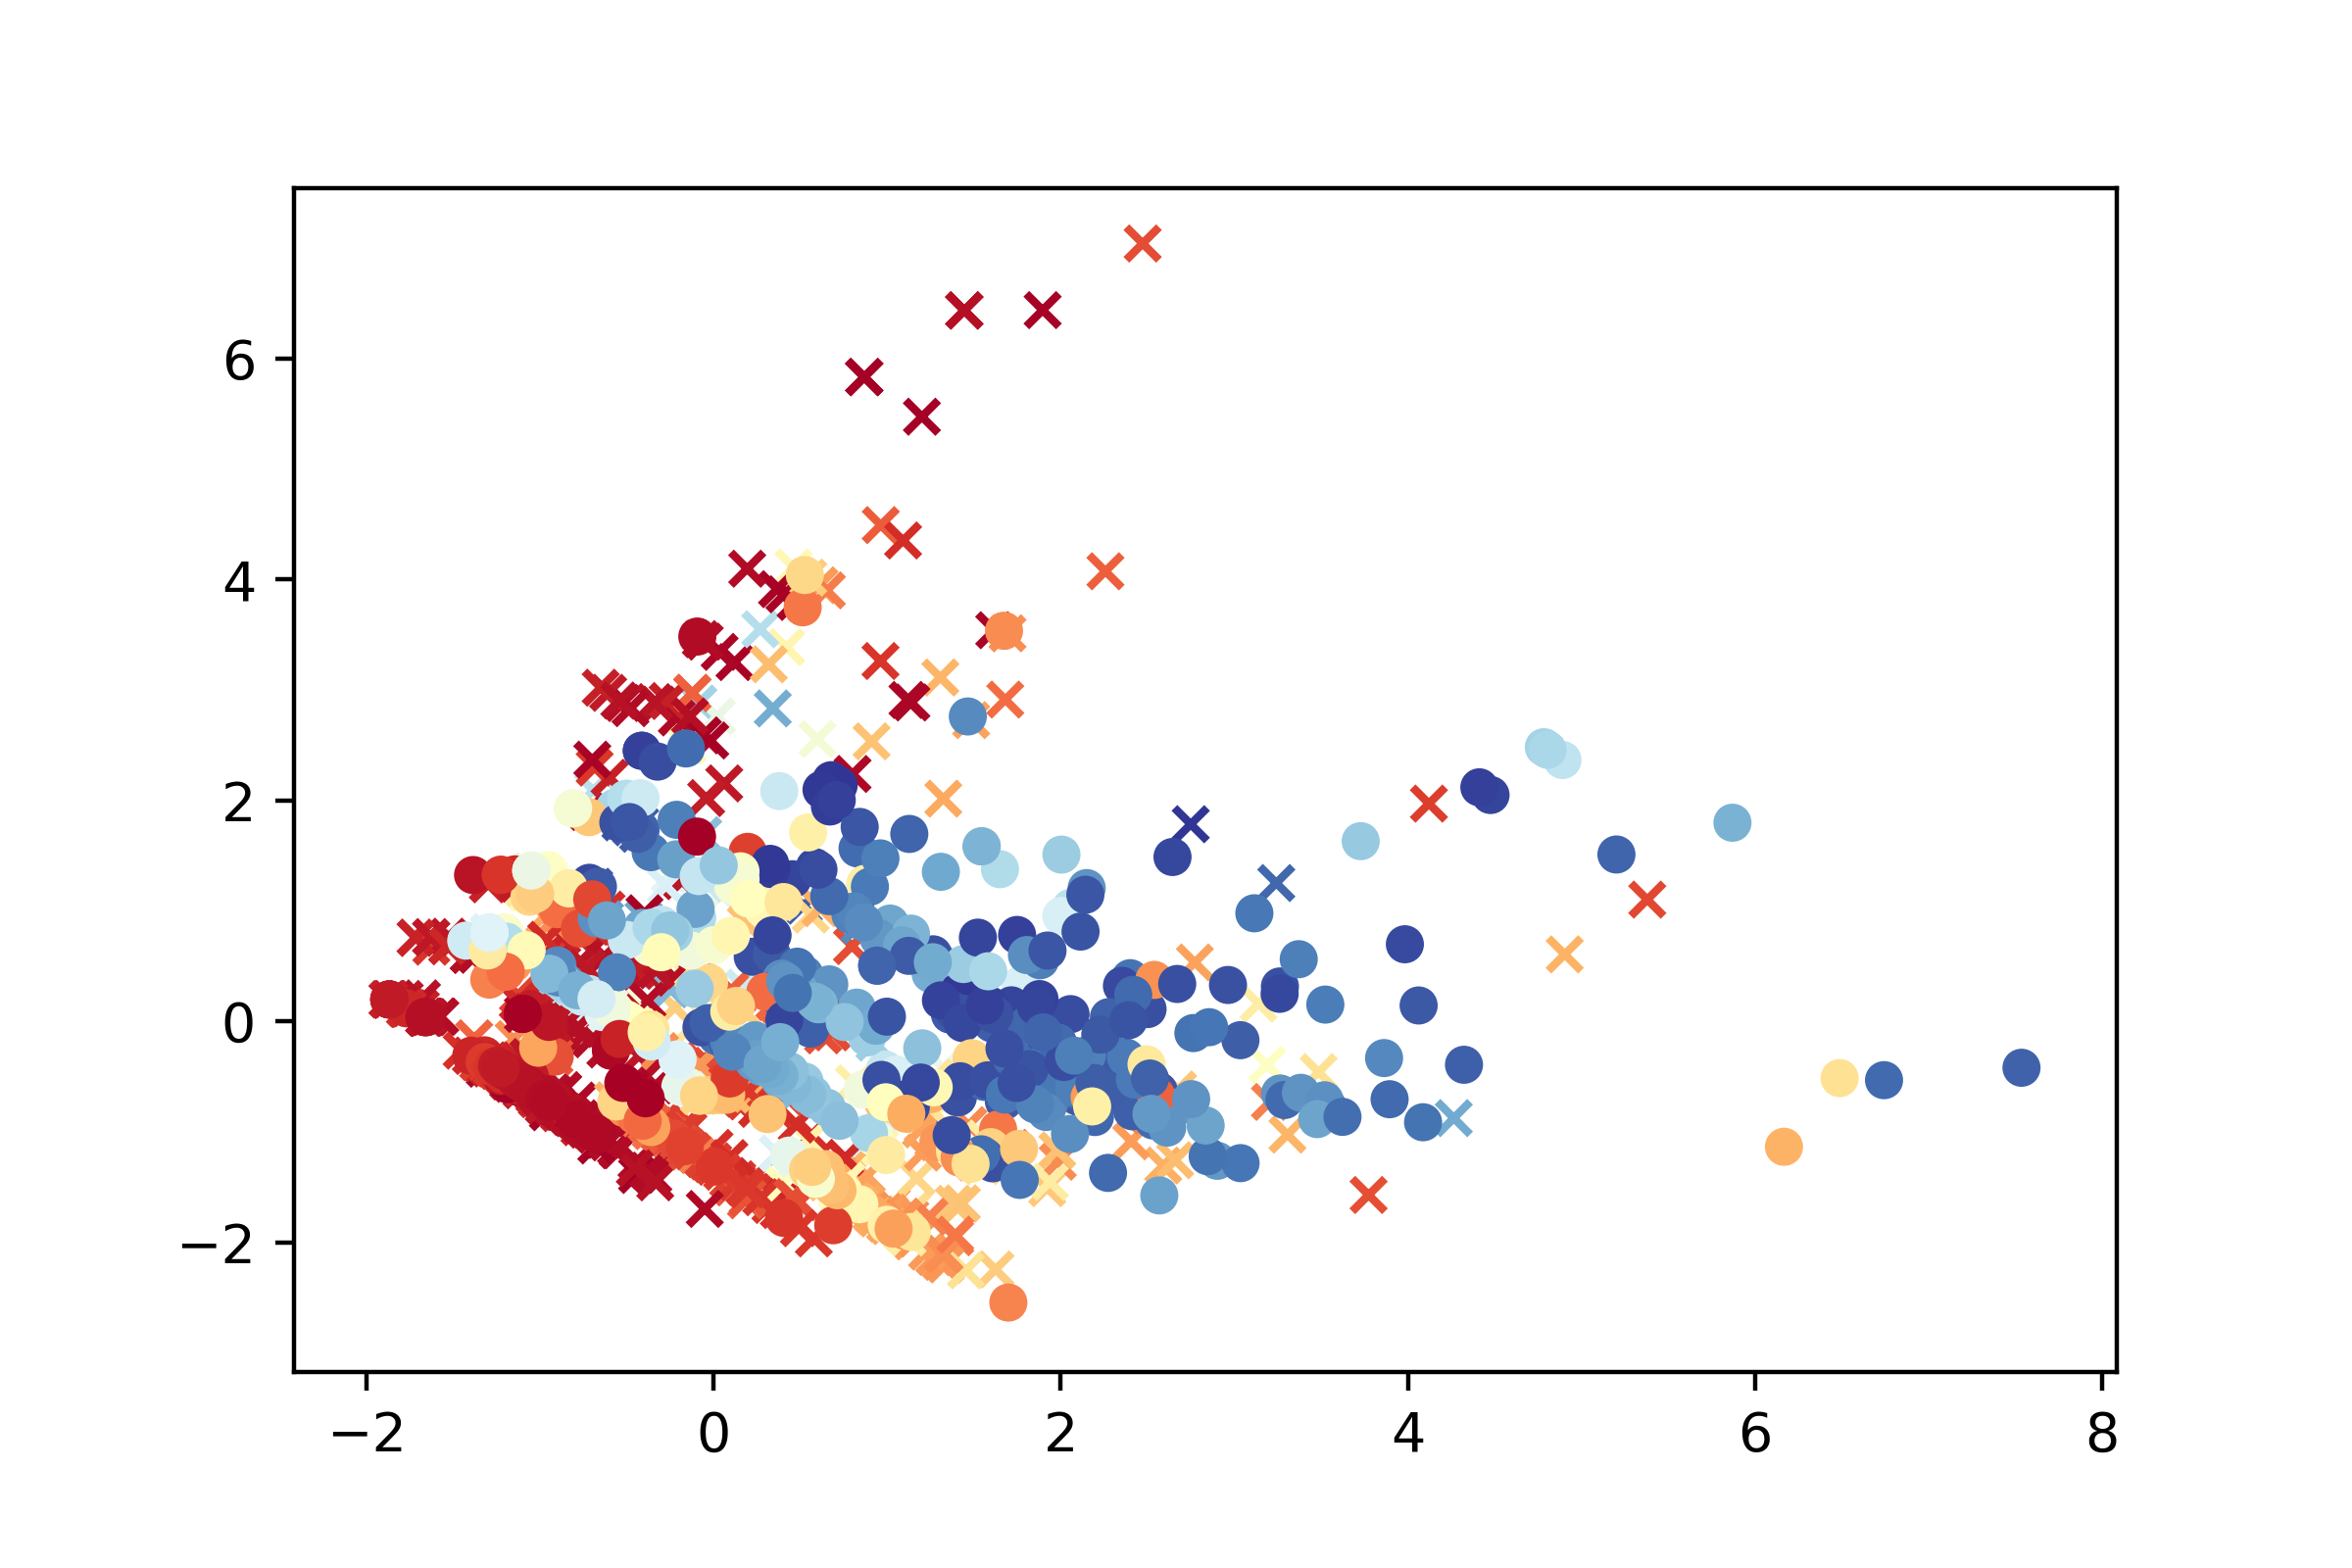
\includegraphics[width=0.22\textwidth]{fig/plt/ti.png} &
%     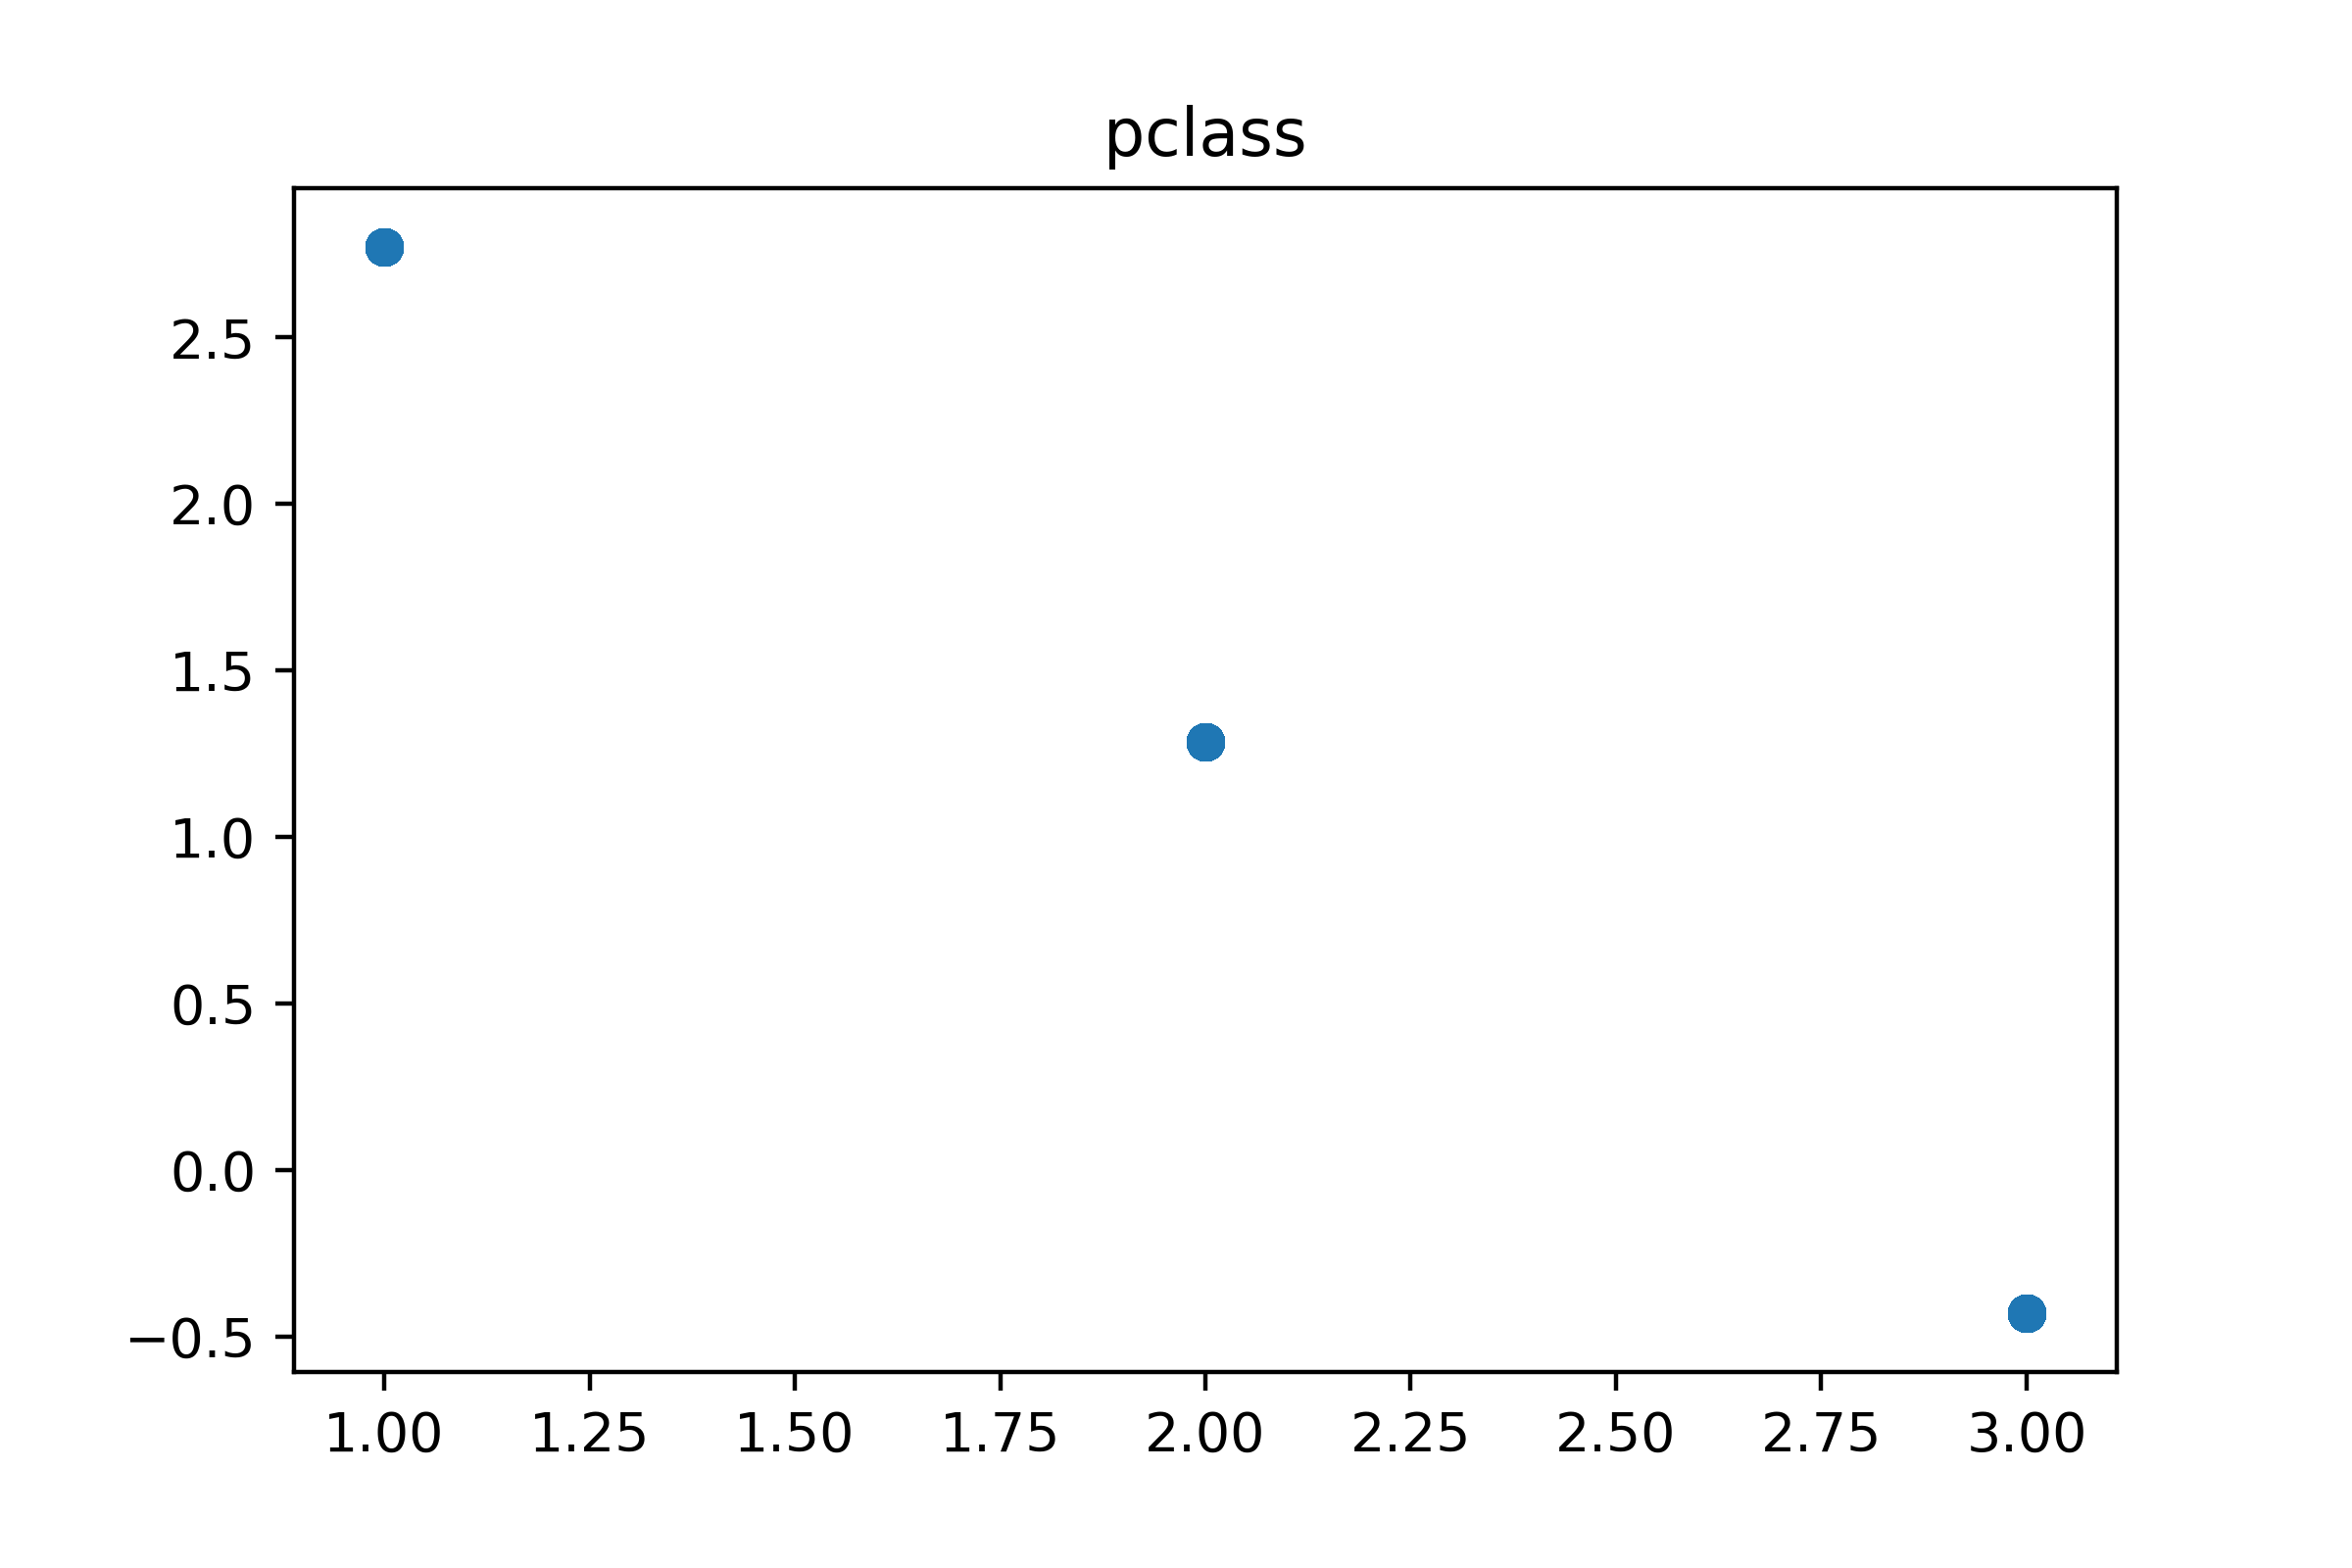
\includegraphics[width=0.40\textwidth]{fig/mnl/ti1.png} &
%     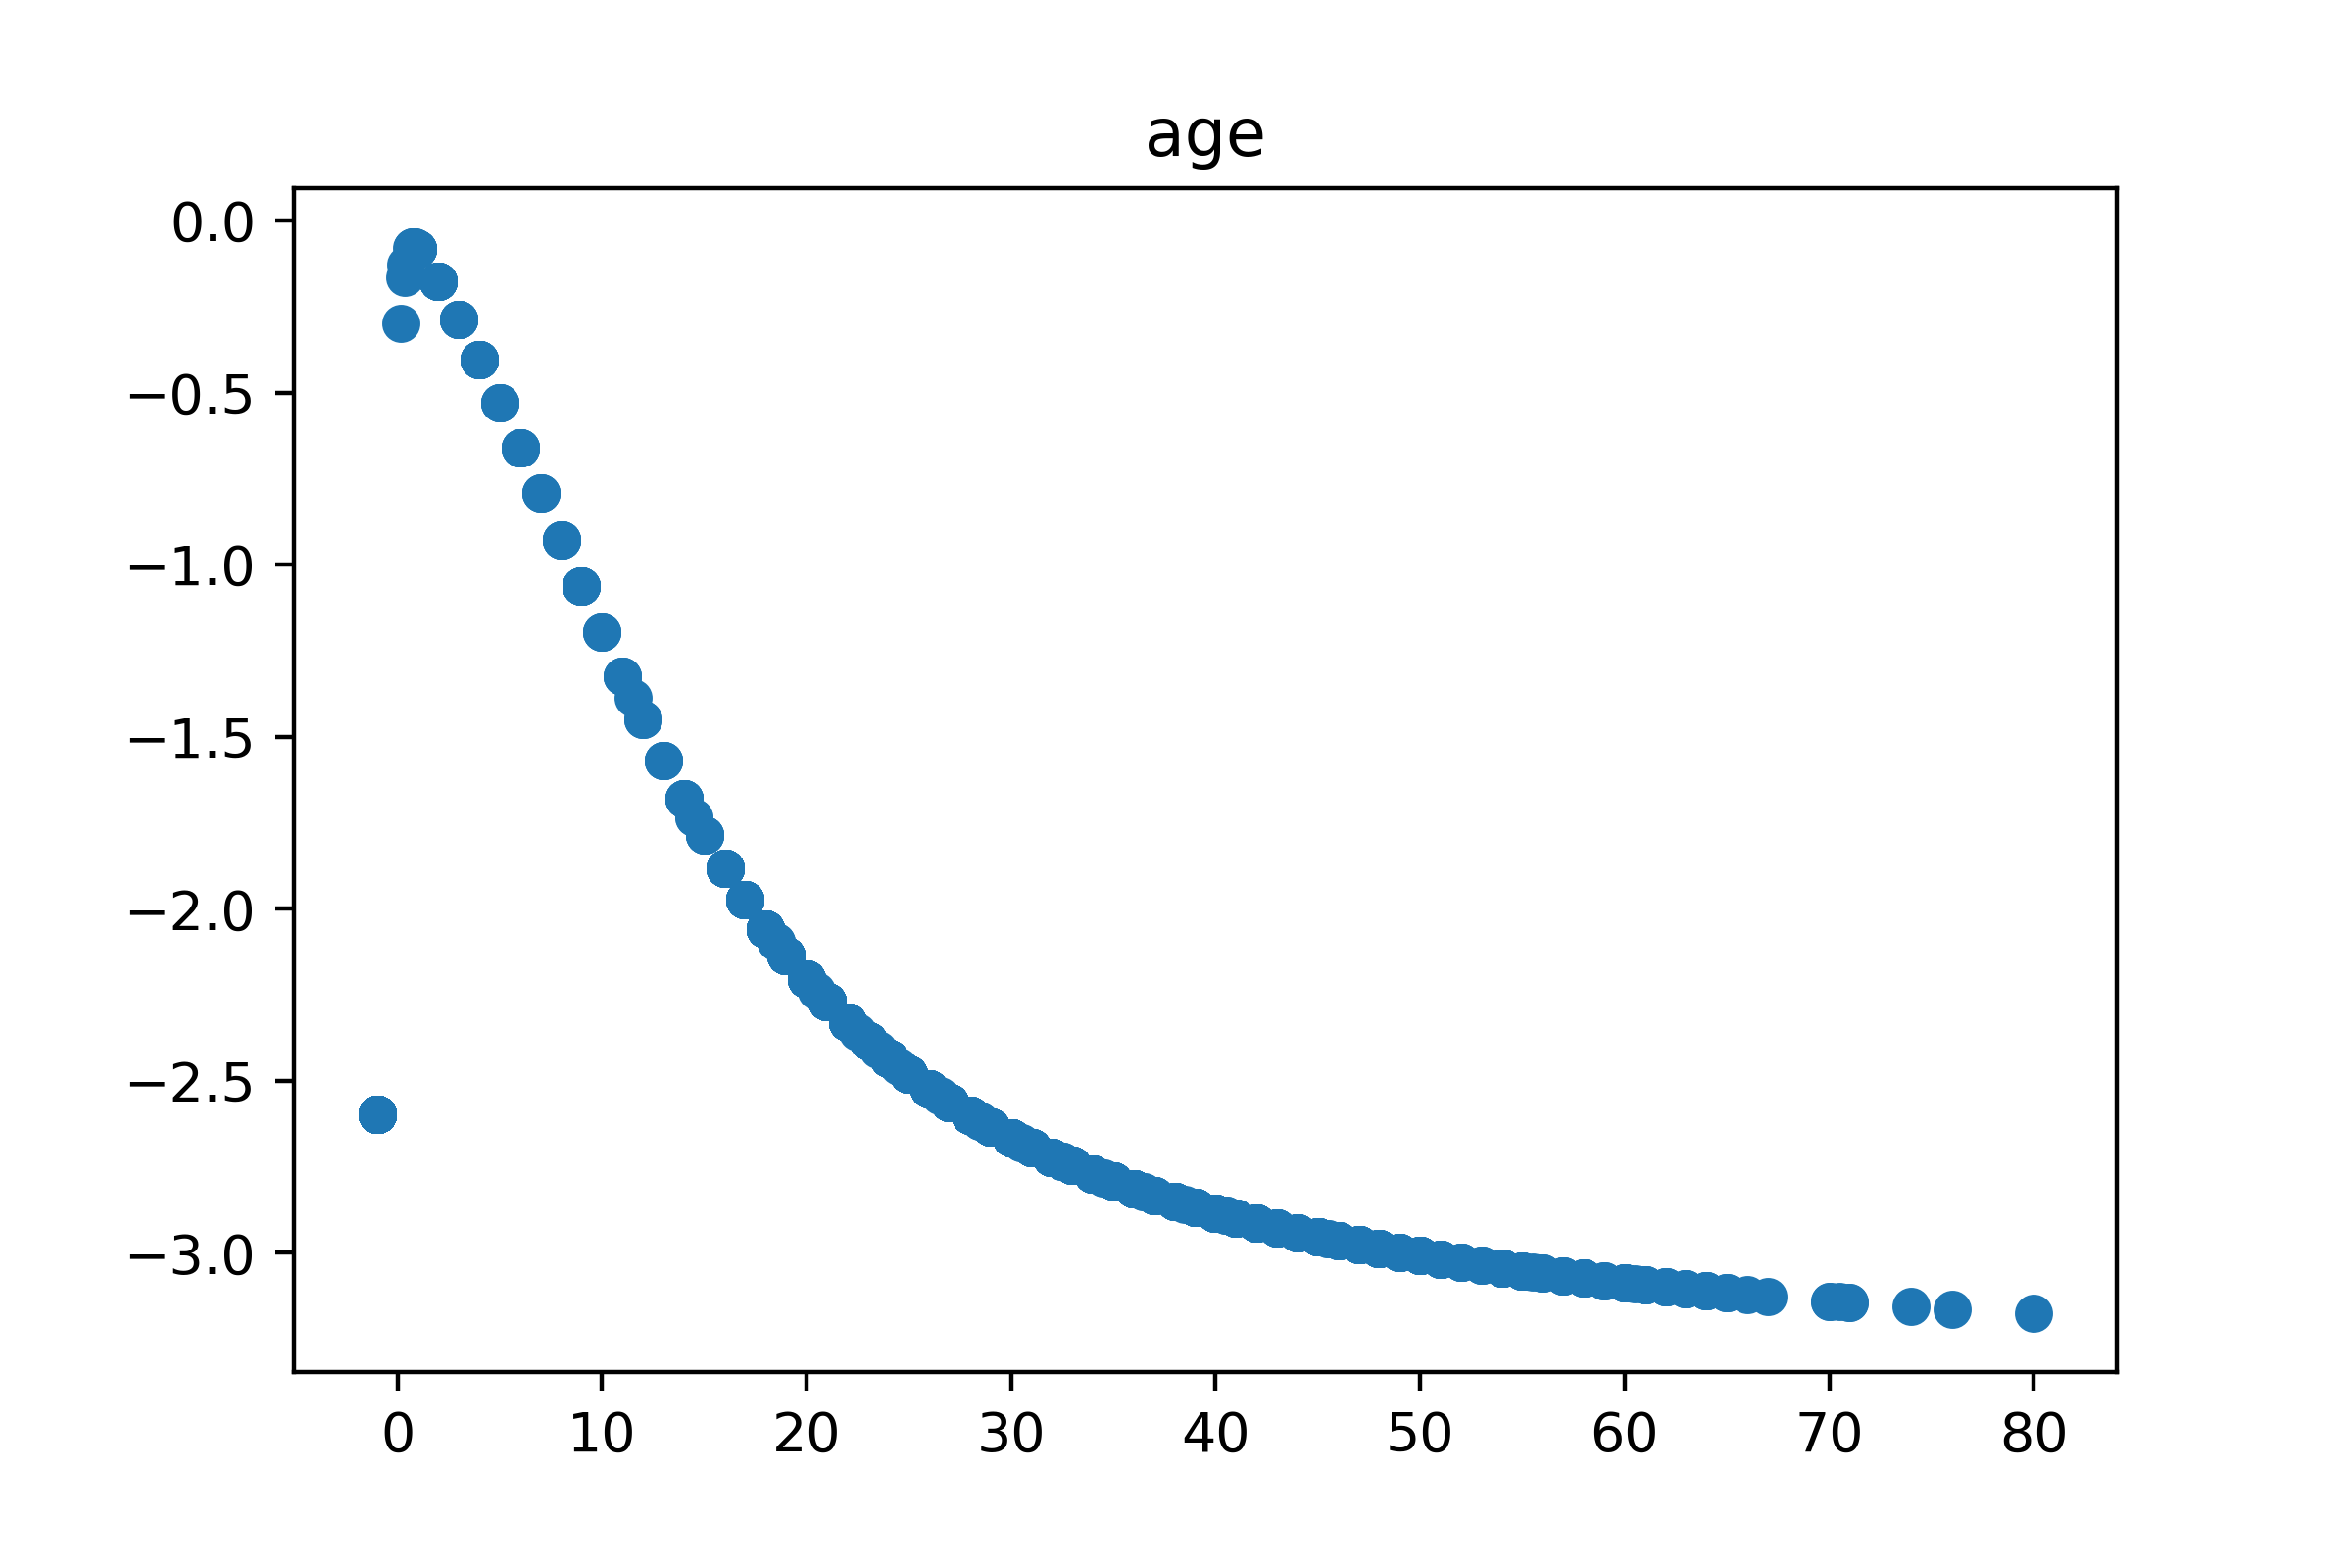
\includegraphics[width=0.40\textwidth]{fig/mnl/ti2.png}\tabularnewline
    
%     Wine & 
%     %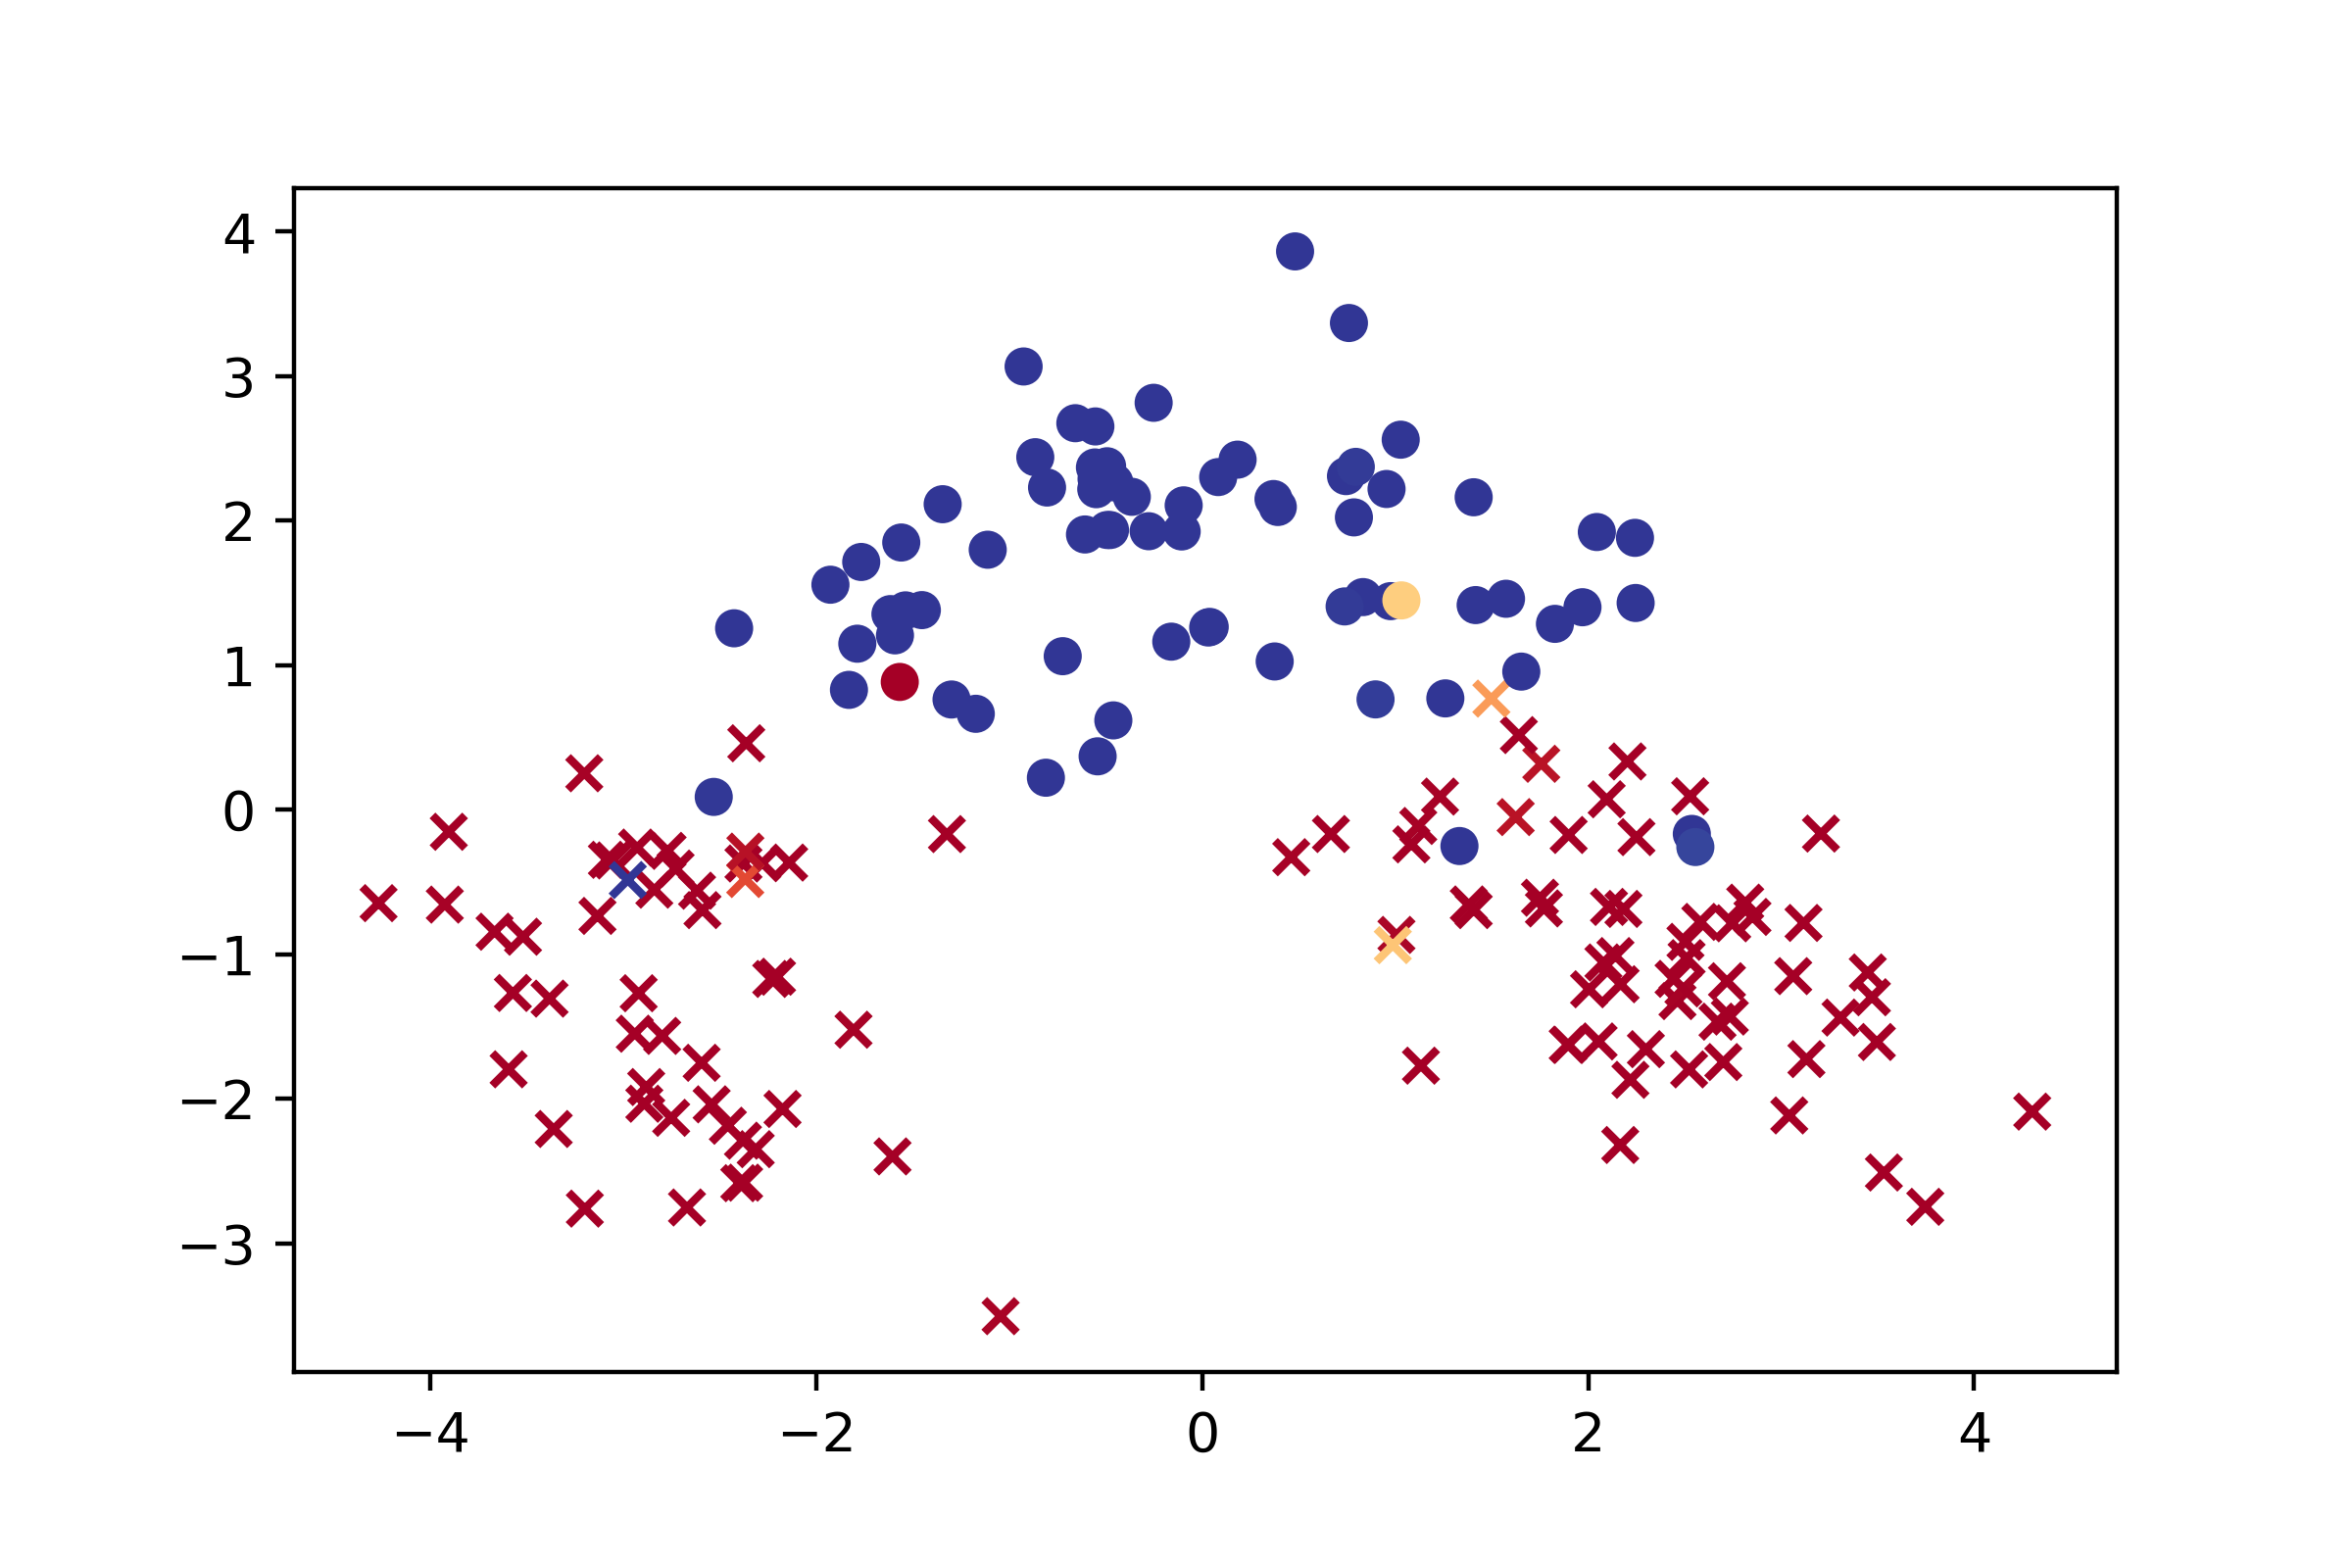
\includegraphics[width=0.22\textwidth]{fig/plt/wi.png} &
%     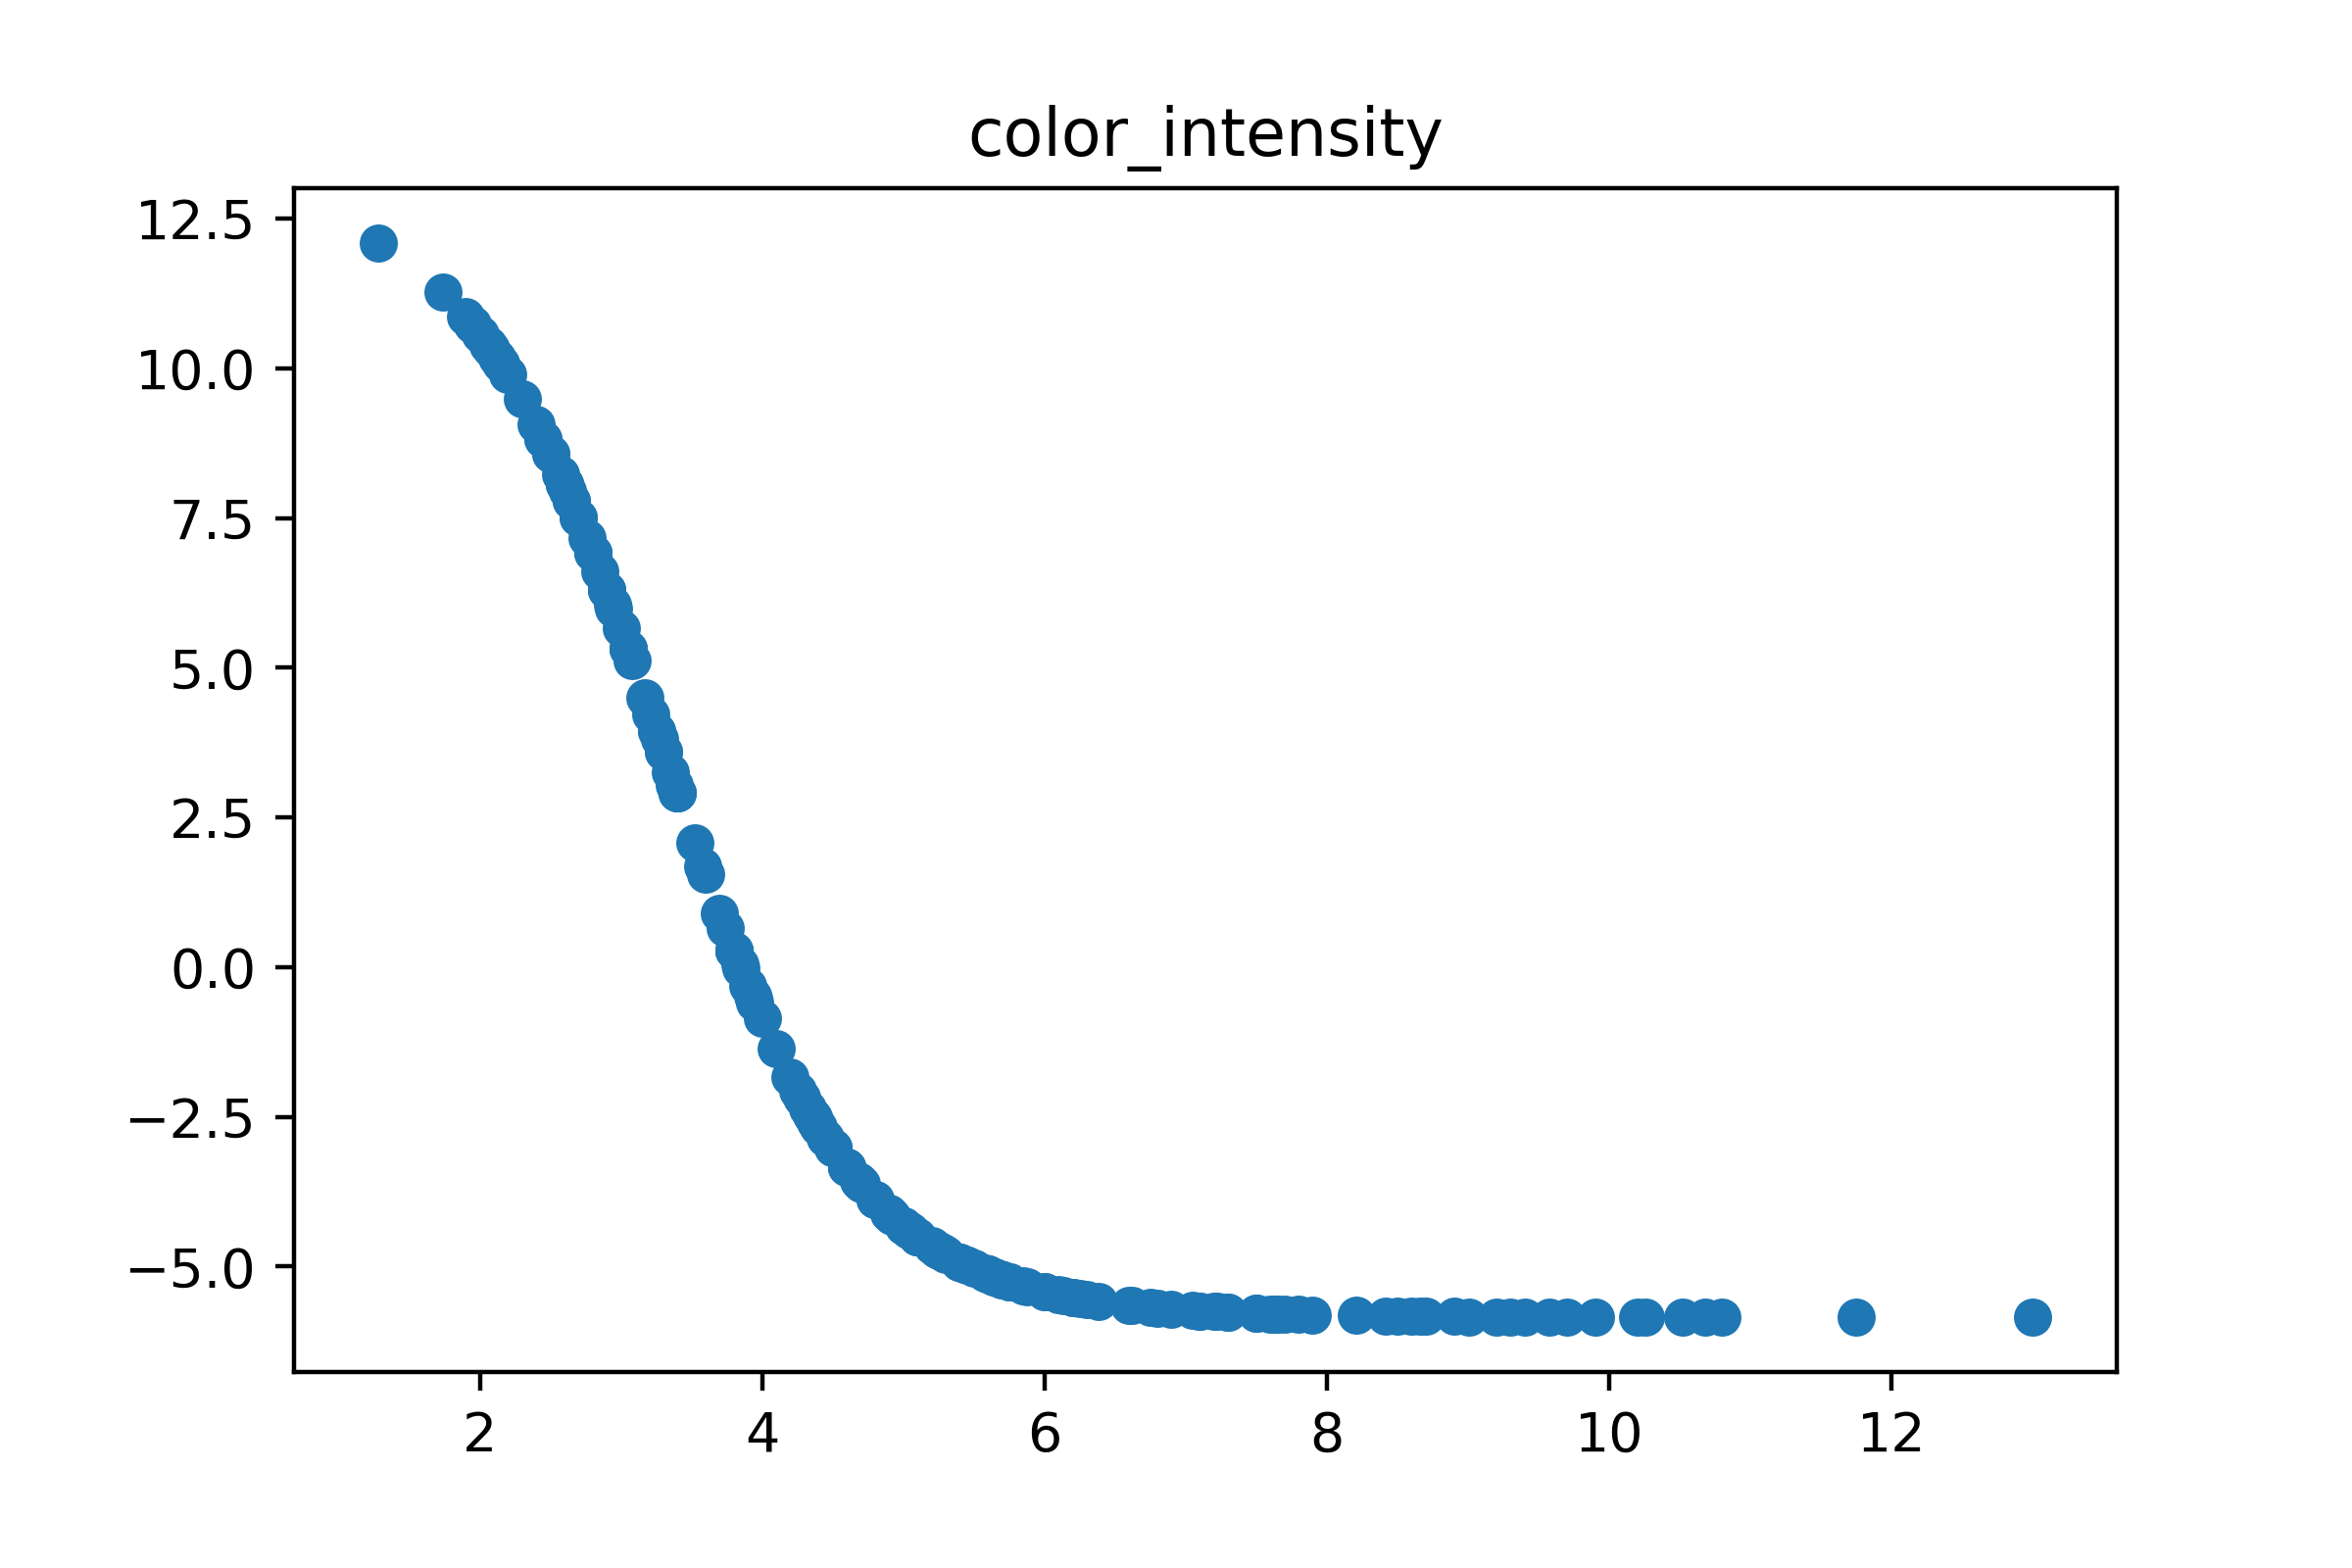
\includegraphics[width=0.40\textwidth]{fig/mnl/wi1.png} &
%     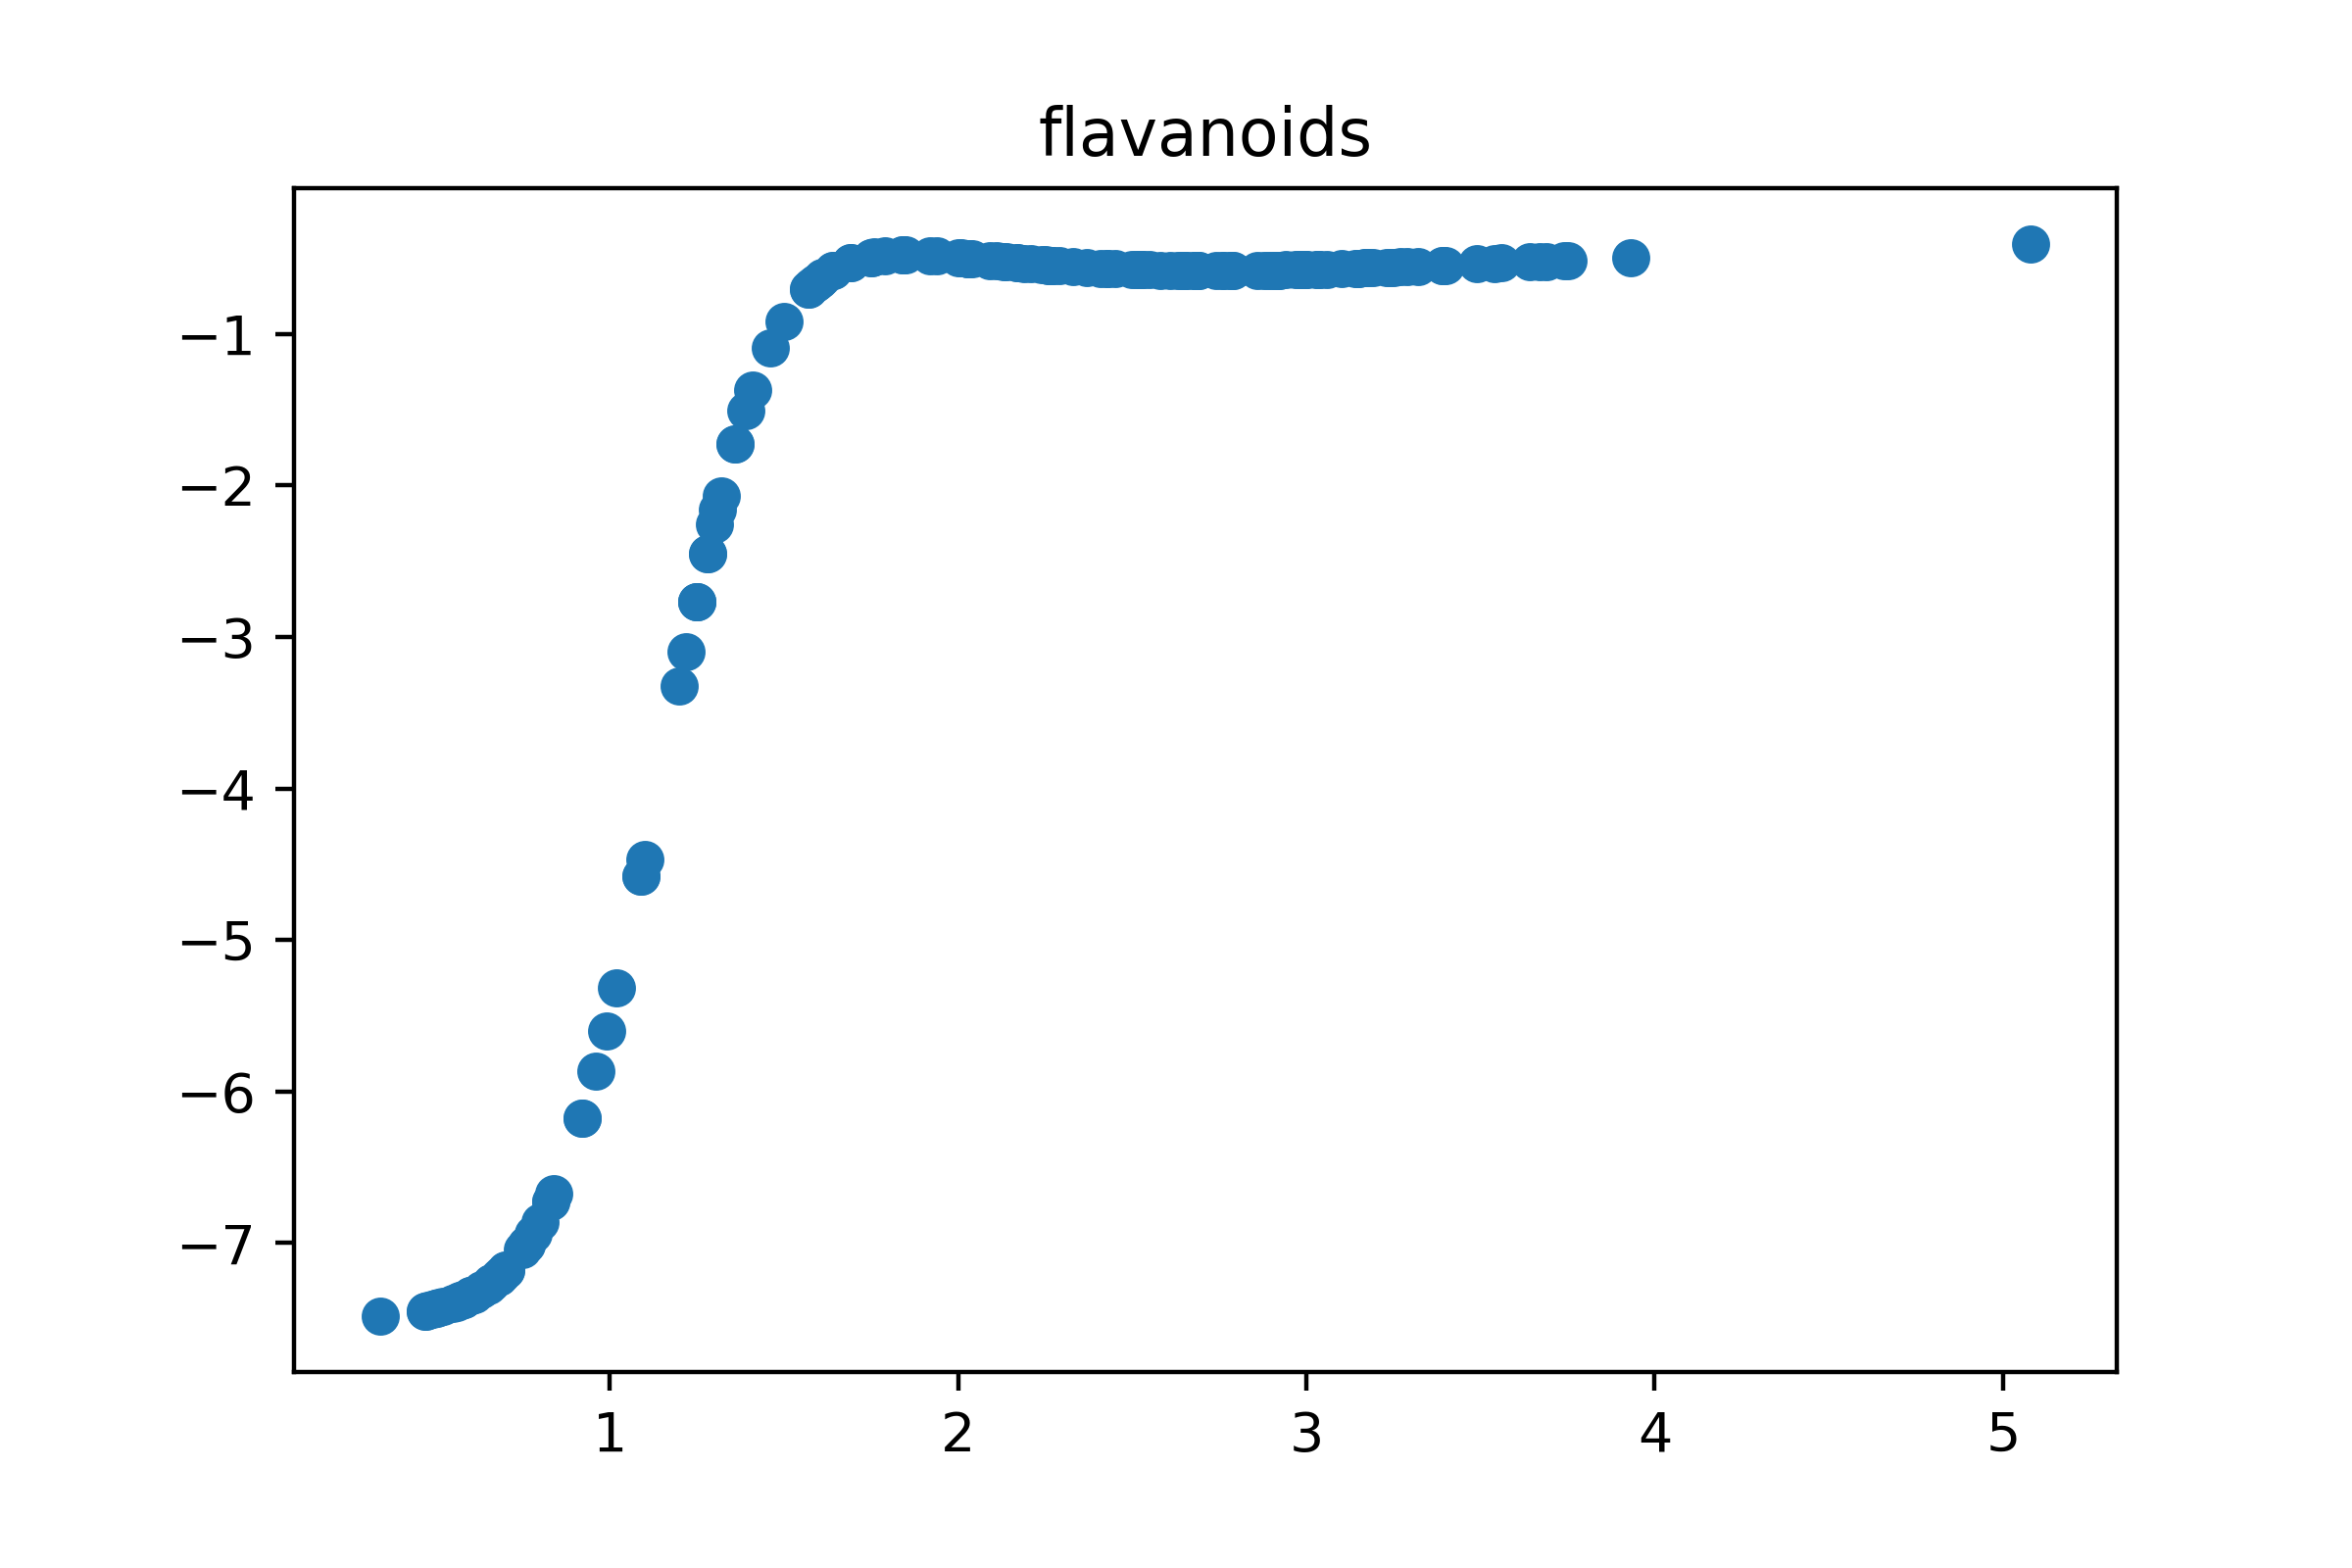
\includegraphics[width=0.40\textwidth]{fig/mnl/wi2.png}\tabularnewline
    
%     % Circle & 
%     % 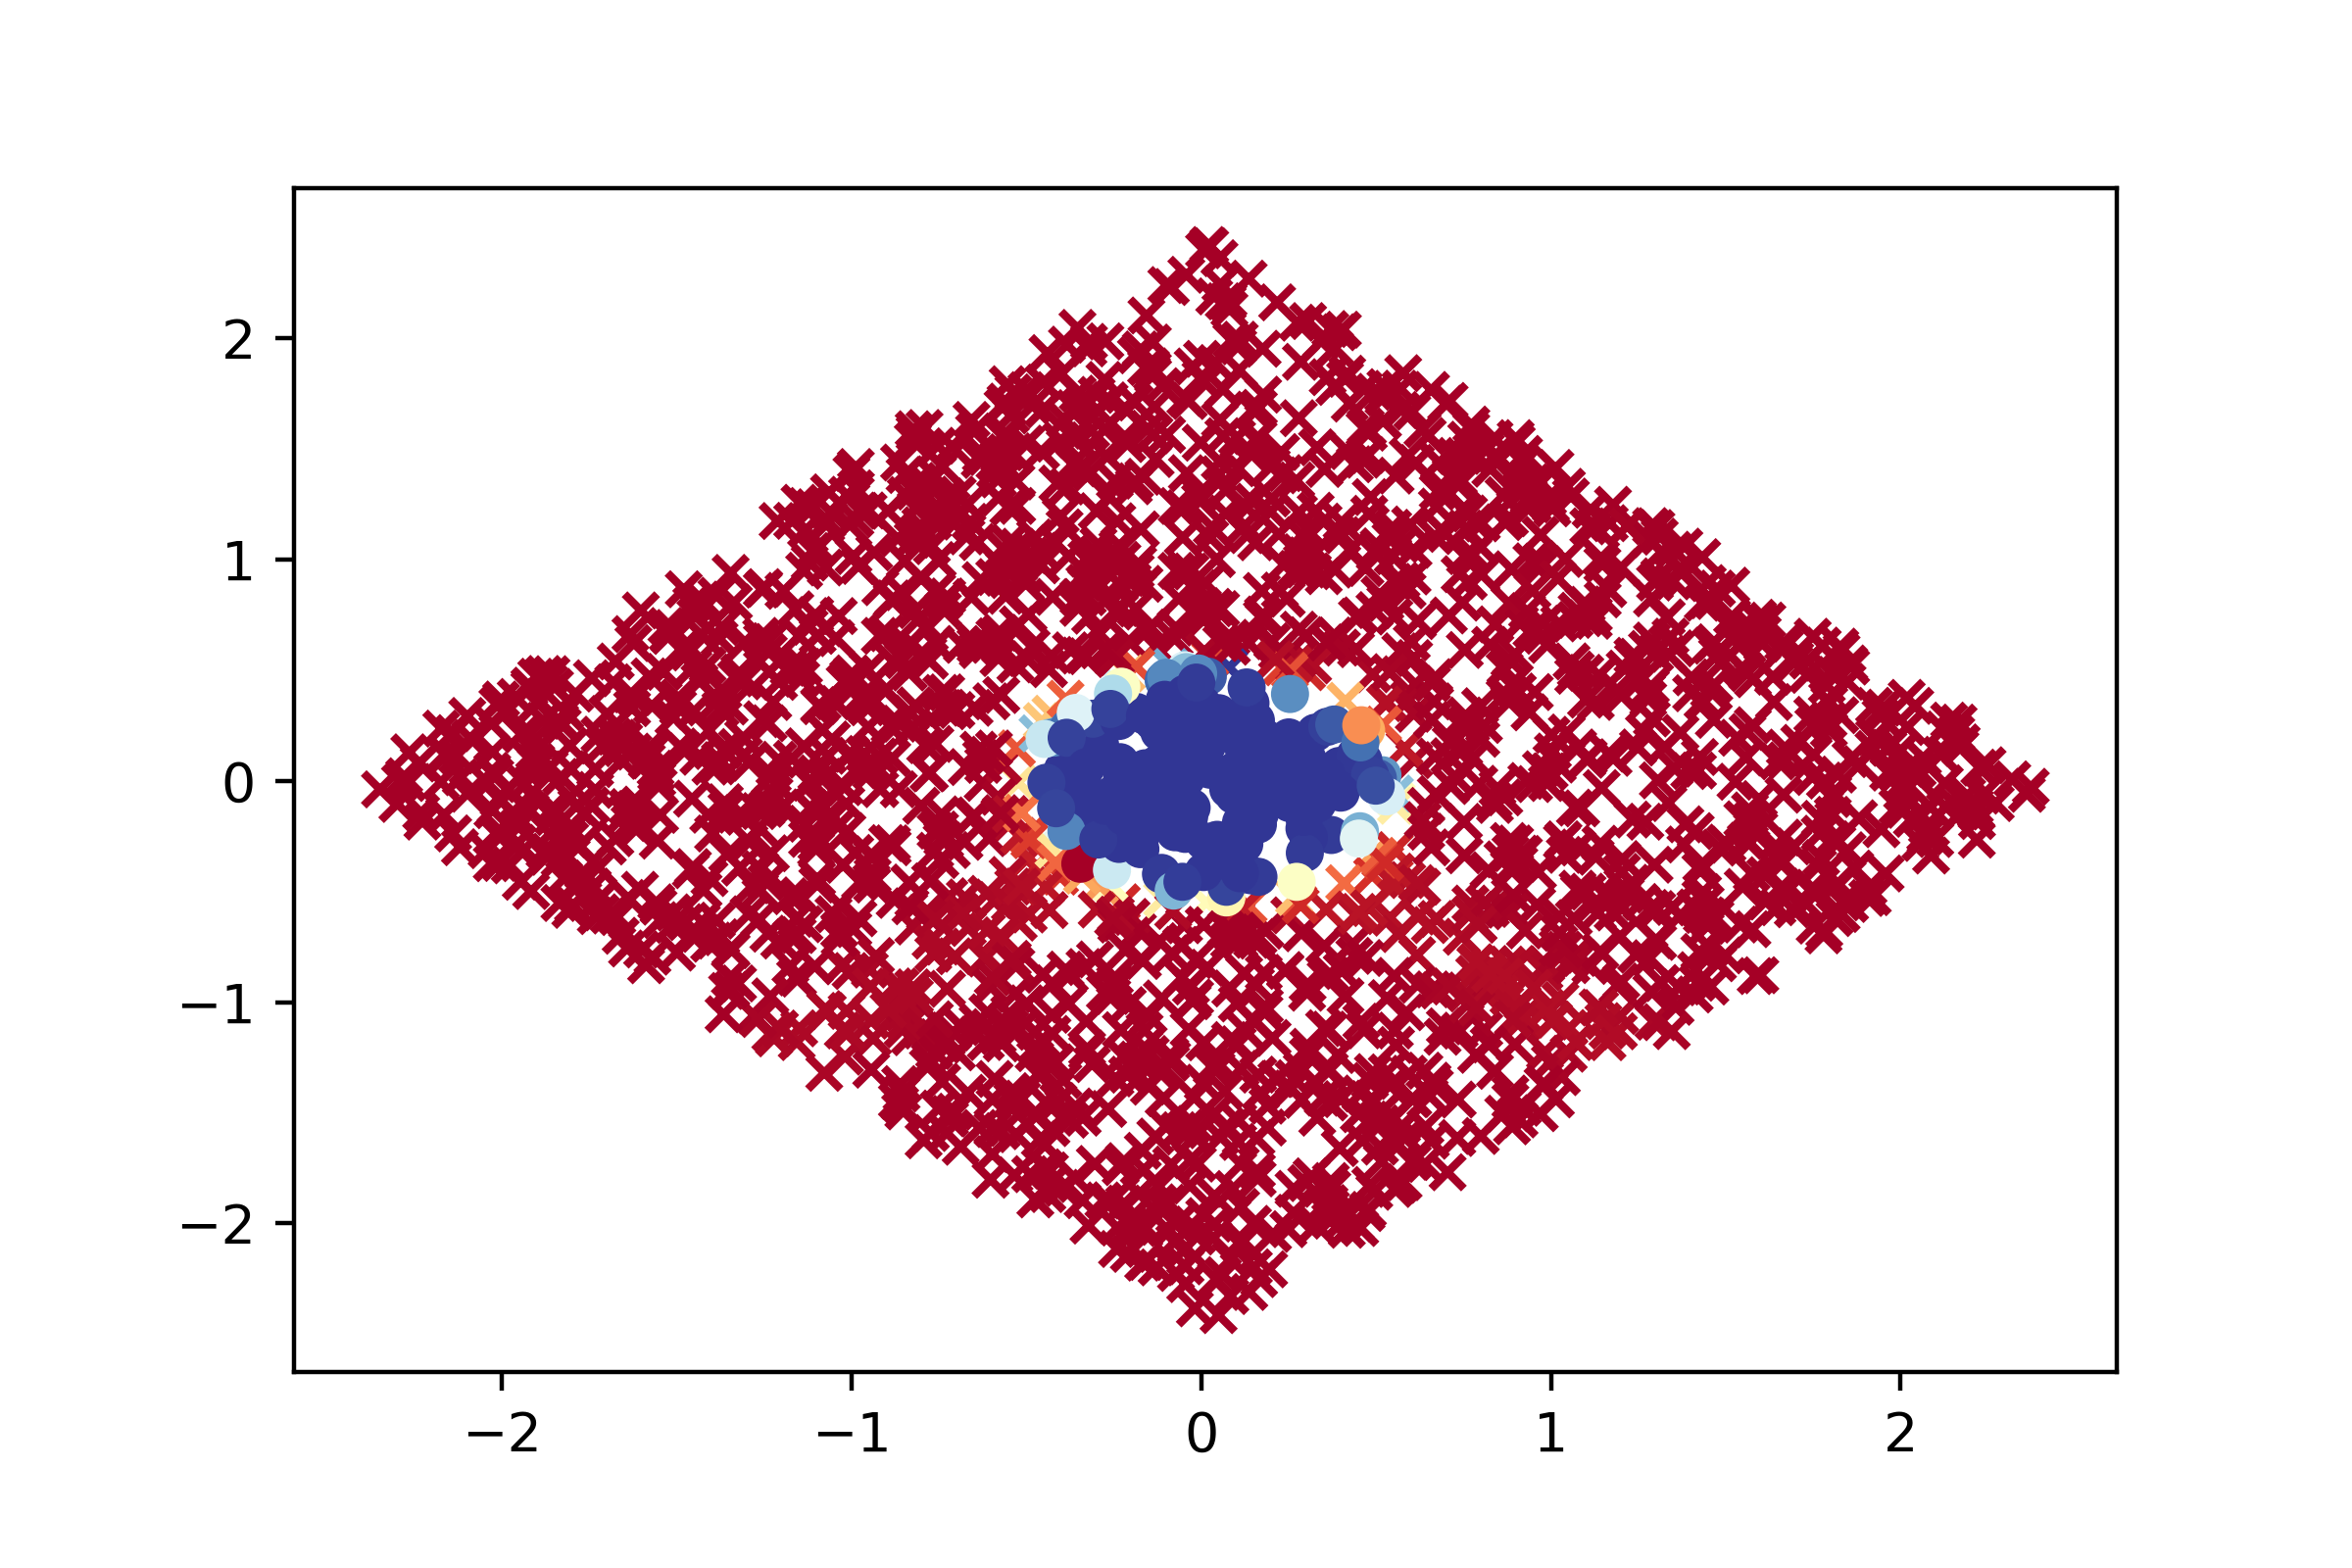
\includegraphics[width=0.22\textwidth]{fig/plt/ci.png} &
%     % \includegraphics[width=0.22\textwidth]{fig/mnl/ci1.png} &
%     % \includegraphics[width=0.22\textwidth]{fig/mnl/ci2.png}\tabularnewline
    
%     % Ellipse & 
%     % \includegraphics[width=0.22\textwidth]{fig/plt/el.png} &
%     % \includegraphics[width=0.22\textwidth]{fig/mnl/el1.png} &
%     % \includegraphics[width=0.22\textwidth]{fig/mnl/el2.png}\tabularnewline
    
%     % XOR & \includegraphics[width=0.22\textwidth]{fig/plt/xr.png} &
%     % \includegraphics[width=0.22\textwidth]{fig/mnl/xr1.png} &
%     % \includegraphics[width=0.22\textwidth]{fig/mnl/xr2.png}\tabularnewline

%     \bottomrule
    
%     \caption{Selected assortment of marginal functions for each dataset. The x-axis represents the domain on the input variable and the y-axis represents the pre-sigmoid contribution to the response.}

% \end{longtable}

\subsection{Analysis}

Results from this experiment support our hypotheses that our network architecture outperforms logistic regression while falling slightly short of GBMs in most real world datasets. In three out of the five datasets tested, our architecture was statistically significantly better than logistic regression and in the remaining two, the results were not statistically significant either way. GBMs outperformed our architecture in the iris dataset, and there was no statistical difference in the remaining four.  

In each of the datasets, our network was able to pull out pertinent non-linear features and incorporate them into the network prediction. The lack of joint terms had surprisingly little impact on the accuracy of the network, as illustrated by the nearly identical performance of our network with the more powerful GBM. This result suggests that, for real-world classification problems, joint terms are often unnecessary, and it is possible to increase interpretability without sacrificing accuracy by employing a GAM-like delinearization approach in this class of problem. 

A more thorough breakdown of each of the datasets is provided in the following section. 

\subsection{Sloan Sky Survey}

In the Sloan Sky Survey dataset, logistic regression performed poorly with an f1 score of 0.6586. Our network performed much better with an f1 score of 0.9864, falling just short of the GBM’s score of 0.9871. The score difference between the network and the GBM was not statistically significant. This dataset was the largest tested and contains very non-linear features, making it an ideal target for GBMs.  Therefore, its promising that our model was able to keep pace, only missing the GBM's performance by a handful of instances. 

Our architecture found a number of important non-linear features in this dataset, the most significant being red-shift. In astronomy, red-shift acts as a proxy for distance, and is intuitively one of the best ways to separate classes of astronomical objects. The relevant non-linearity exhibited a large spike at low-mid ranges of red-shift, suggesting that Galaxies occur most frequently at a distance between stars and quasars, which they do.

The network picked up on additional non-linear features such as declination angle, and a number of approximately linear features such as the g, i, and r bands. The network also zeroed out a number of unimportant variables, including the mjd, object id, and plate. This zeroing effect illustrates that our architecture is capable of performing automatic data-driven feature selection.

\subsection{Breast Cancer}

In the breast cancer dataset, the objective is to separate malignant and benign tumors using a set of input variables. This dataset is considerably smaller than the stellar dataset, but contains more highly correlated features. In this dataset, the our network outperformed the GBM with an f1 score of 0.9512 to 0.9383, however this difference was not statistically significant. The small sample size and large feature set made it more difficult not to overfit GBM, explaining the slightly lower score. Again, our target variable was not linearly separable, so logistic regression performed poorly with a f1 score of 0.3592, this result was statistically significant. 

Our network found a number of important non-linear features, including concavity worst, texture worst, and symmetry worst. It also selected out a number of uninformative features, such as the patient id. This dataset demonstrates that the decrease in power from dropping the network's joint terms does not always negatively impact the performance of the model. On the contrary, by dropping the joint terms from the network, we made it significantly less able to overfit, which actually improved the network's performance. 

\subsection{Small Datasets}

In addition to the two larger datasets above, we also tested our method on three smaller datasets: Iris, Titanic, and Wine. These datasets are all small-scale classification problems, containing only a few dozen samples in each category. Wine is notable for being almost linearly separable, and Titanic is notable for being very noisy.

\paragraph{Iris:} In the Iris dataset, our architecture significantly outperformed logistic regression while slightly under-performing the GBM. Both differences were statistically significant. The most important classification features were petal length and petal width, which both exhibited significant marginal non-linearities. 

\paragraph{Titanic:} In the Titanic dataset, all three methods performed similarly, with logistic regression and GBMs slightly outperforming the marginal network. The marginal network picked up the important input variables class, age, and sex, suggesting that women, children, and first-class passengers had the best chance of survival. This analysis corresponds with the real-world understanding of the disaster, where women, children, and first-class passengers were given priority in boarding the life boats.

\paragraph{Wine:} In the wine dataset, logistic regression slightly outperformed our architecture with f1 score of 0.9231 to 0.9189. GBMs fared worse with an f1 score of 0.8718, but none of these differences are statistically significant. Most terms identified by our network are linear, while the remaining two are linear over a domain and zero elsewhere. This observation suggests that a linear model may be the best approach for this dataset. GBMs under-performed due to the large input dimension (12) over a small number of samples (130), making it more difficult to avoid over-fitting.
